
\chapter{Introducción a las Ecuaciones Diferenciales  }
%\addtocontents{toc}{\protect\figuretoc{1}}
\minitoc

\begin{tikzpicture}[remember picture,overlay]
	\node[anchor=east,inner sep=20pt] at (current page text area.west|-,20cm) {\includegraphics[height=5cm]{1}};
\end{tikzpicture}
%\addtocontents{toc}{\protect\marginnote{\vskip-9mm\includegraphics[width=3cm]{example-image}}}

%\BackImage[width=.5\textwidth]{1}% image on page 1

\section{Definiciones y terminología }

\Definition{Ecuación Diferencial}{Se dice que una ecuación diferencial (ED) es cualquier ecuación que contiene las derivadas de una o más variables dependientes con respecto a una o más variables independientes.}\label{def:Definicion}

\begin{marginfigure}
	\centering
	\subcaptionbox{Notación Lagrage}
	{\includegraphics[width=\marginparwidth]{Imagen/Lagrage.pdf}}\\
	\subcaptionbox{Notación Leibniz}
	{\includegraphics[width=\marginparwidth]{Imagen/Leibniz.pdf}}\\
	\subcaptionbox{Notación Jacoby}
	{\includegraphics[width=\marginparwidth]{Imagen/Jacoby.pdf}}
	\subcaptionbox{Notación Cauchy}
	{\includegraphics[width=\marginparwidth]{Imagen/Cauchy.pdf}}
	\caption{Notación de algunas derivas segun algunos autores}
	
\end{marginfigure}


Las siguientes ecuaciones  son ejemplos de ecuaciones diferenciales.

\begin{eqnarray*}
	% \nonumber % Remove numbering (before each equation)
	\displaystyle\frac{d^{2}y}{dx^{2}}+4\displaystyle\frac{dy}{dx}= \sin{x} \hspace{2cm} \displaystyle x^{2}\frac{d^{2}y}{dx^{2}}+\displaystyle x\frac{dy}{dx}+\displaystyle(x^{2}-\nu^{2})y=0
\end{eqnarray*}
\begin{eqnarray*}
	% \nonumber % Remove numbering (before each equation)
	\displaystyle\frac{\partial^{2}u(x,y)}{\partial x^{2}}+\displaystyle\frac{\partial^{2}u(x,y)}{\partial y^{2}}= 0 \hspace{1cm}  \displaystyle C\frac{\partial^{2}u(x,t)}{\partial x^{2}}=\displaystyle\frac{\partial u(x,t)}{\partial t}
\end{eqnarray*}


Con el objetivo de referirnos a las ecuaciones diferenciales (ED), debemos clasificarla por \textbf{Tipo, Linealidad y Orden}.

\subsection*{Clasificación por Tipo}

Si una ecuaci\'on diferencial contiene \'unicamente derivadas ordinarias de una o m\'as variables dependientes con respecto a una sola variable independiente, se dice que es una \textbf{ecuaci\'on diferencial ordinaria (EDO)}. Por ejemplo,

\begin{eqnarray}\label{EDO1}
	% \nonumber % Remove numbering (before each equation)
	\displaystyle\frac{d^2 y}{d x^2}-\frac{d y}{d x}+6 y=0 \hspace{1cm} y \hspace{1cm} \displaystyle\frac{d x}{d t}+\displaystyle\frac{d y}{d t}=2 x+y
\end{eqnarray}

\vspace{0.5cm}

son ecuaciones diferenciales ordinarias. Una ecuaci\'on diferencial que contiene derivadas parciales de una o m\'as variables dependientes de dos o m\'as variables independientes se llama \textbf{ecuaci\'on diferencial parciales (EDP)}. Por ejemplo,

\begin{eqnarray}\label{EDP1}
	% \nonumber % Remove numbering (before each equation)
	\displaystyle\frac{\partial^2 u(x,y)}{\partial x^2}=\displaystyle\frac{\partial^2 u(x,y)}{\partial t^2}-2 \frac{\partial u(x,y)}{\partial t} \quad \text { y } \quad \displaystyle\frac{\partial u(x,y)}{\partial y}=\displaystyle-\frac{\partial v}{\partial x}
\end{eqnarray}

son ecuaciones diferenciales parciales.

\vspace{0.5cm}

\textbf{Notaci\'on}\\
HACER AHORA

\subsection*{Clasificaci\'on por Orden}
El orden de una ecuaci\'on diferencial (EDO o EDP) representa el orden de la derivada m\'as alta presente en la ecuaci\'on. Por ejemplo, las siguientes ecuaciones son de orden $3,1\,\text{y}\, 2$  respectivamente.

\begin{eqnarray*}
	% \nonumber % Remove numbering (before each equation)
	x^3 \displaystyle\frac{d^3 y}{d x^3}+2 x^2\displaystyle \frac{d^2 y}{d x^2}-x\displaystyle \frac{d y}{d x}+y&=&12 x^2 \\
	(y-x)\displaystyle y^{\prime}&=&y-x+8 \\
	\displaystyle\frac{d^2 y}{d x^2}&=&\displaystyle\sqrt{1+\left(\frac{d y}{d x}\right)^3}
\end{eqnarray*}

\marginpar{\includegraphics[width=\marginparwidth]{Imagen/Orden.pdf}}

En ocasiones las ecuaciones diferenciales se escriben en la forma diferencial $\textbf{M(x,y)dx+N(x,y)dy=0}$. En el siguiente ejemplo supondremos que y representa la variable dependiente



\begin{eqnarray*}
	% \nonumber % Remove numbering (before each equation)
	2 x y d x+\left(x^2-1\right) d y&=&0
\end{eqnarray*}
Sabemos que $dy=y^{\prime}dx$, as\'i la expresi\'on anterior se puede expresar como
\begin{eqnarray*}
	% \nonumber % Remove numbering (before each equation)
	2 x y d x+\left(x^2-1\right)y^{\prime}dx&=&0\\
	\left(2 x y +\left(x^2-1\right)y^{\prime}\right)dx&=&0\\
	2xy+\left(x^2-1\right)y^{\prime}&=&0
\end{eqnarray*}
De manera simb\'olica, es posible expresar una ecuaci\'on diferencial ordinaria de $n$-\'esimo orden como una variable dependiente empleando la forma general
\begin{eqnarray}\label{EDGF}
	F\left(x, y, y^{\prime}, \ldots, y^{(n)}\right)&=&0
\end{eqnarray}
donde $F$ es una funci\'on con valores reales de $n+2$ variables: $x, y, y^{\prime}, \ldots, y^{(n)}$. Por motivos pr\'acticos como te\'oricos, de aqu\'i en adelante debemos suponer que es posible resolver una ecuaci\'on diferencial ordinaria presentada en la forma (\ref{EDGF}) \'unicamente para la derivada m\'as alta $y^{(n)}$ en t\'erminos de las variables $n+1$ restantes. La ecuaci\'on diferencial
\begin{eqnarray}\label{formanormal}
	% \nonumber % Remove numbering (before each equation)
	\displaystyle \frac{d^n y}{d x^n}&=&\displaystyle f\left(x, y, y^{\prime}, \ldots, y^{(n-1)}\right)
\end{eqnarray}
donde $f$ es una funci\'on continua con valores reales, se denomina forma normal de (\ref{EDGF}). Para el caso de las ecuaciones diferenciales ordinarias de primer, segundo y tercer orden, se expresan de las siguientes formas

\begin{eqnarray}\label{primerorden}
	% \nonumber % Remove numbering (before each equation)
	\displaystyle\frac{d y}{d x}&=&f\left(x,y\right) \
\end{eqnarray}
\begin{eqnarray}\label{ED11}
	\displaystyle\frac{d^2 y}{d x^2}&=&f\left(x, y, y^{\prime}\right)
\end{eqnarray}
\begin{eqnarray}\label{ED111}
	\displaystyle\frac{d^3 y}{d x^3}=f\left(x, y, y^{\prime},y^{\prime\prime}\right)
\end{eqnarray}



\Example{
	Expresa la siguiente EDO.
}{
\begin{eqnarray*}
	\left(\tan(x)-\sen(x) \sen(y)\right)d x+\cos(x) \cos(y)dy&=&0
\end{eqnarray*} en la forma normal.

}

\begin{sol}
	Reemplazando el diferencial $dy$
	\begin{eqnarray*}
		\left(\tan(x)-\sen(x) \sen(y)\right)d x+\cos(x) \cos(y)y^{\prime}dx&=&0
	\end{eqnarray*}
	Por linealidad
	\begin{eqnarray*}
		\left[\tan(x)-\sen(x) \sen(y)+\cos(x) \cos(y)y^{\prime}\right]dx&=&0\\
		\tan(x)-\sen(x) \sen(y)+\cos(x) \cos(y)y^{\prime}&=&0
	\end{eqnarray*}
	despejando la derivada de mayor orden
	\begin{eqnarray*}
		% \nonumber % Remove numbering (before each equation)
		y^{\prime} &=&\displaystyle-\frac{\tan(x)-\sen(x) \sen(y)}{\cos(x) \cos(y)}
	\end{eqnarray*}
	donde $f(x,y)=\displaystyle-\frac{\tan(x)-\sen(x) \sen(y)}{\cos(x) \cos(y)}$
	
\end{sol}

\begin{marginfigure}
	\centering
	\subcaptionbox{No lineal $e^y$ }
	{\includegraphics[width=\marginparwidth]{Imagen/e^y.pdf}}\\
	\subcaptionbox{No lineal $y^2 $}
	{\includegraphics[width=\marginparwidth]{Imagen/x^2+y^2.pdf}}\\
	\subcaptionbox{No lineal $sen(y) $}
	{\includegraphics[width=\marginparwidth]{Imagen/sen y.pdf}}
	\caption{Ecuaciones diferenciales no lineales}
	
\end{marginfigure}


\subsection*{Clasificaci\'on por  Linealidad}
Se dice que una ecuaci\'on diferencial ordinaria de $n$-\'esimo orden (\ref{EDGF}) es lineal si $F$ es lineal en $y, y^{\prime}, \ldots, y^{(n)}$. Esto significa que una EDO de $n$-\'esimo orden es lineal cuando la ecuaci\'on (\ref{EDGF}) se puede expresar como
\begin{eqnarray}\label{EDLG}
	% \nonumber % Remove numbering (before each equation)
	a_n(x) y^{(n)}+a_{n-1}(x) y^{(n-1)}+\cdots+a_1(x) y^{\prime}+a_0(x) y&=&g(x)
\end{eqnarray}
Como casos particulares de la expresi\'on (\ref{EDGF}) se obtienen las ecuaciones diferenciales de ordenes $1,2\,\text{y}\, 3$, escogiendo respectivamente $n=1,n=2\, \text{y}\, n=3$
\begin{eqnarray*}
	% \nonumber % Remove numbering (before each equation)
	a_1(x)\displaystyle \frac{d y}{d x}+a_0(x) y&=&g(x) \\
	a_2(x)\displaystyle \frac{d^2 y}{d x^2}+a_1(x) \displaystyle\frac{d y}{d x}+a_0(x) y&=&g(x) \\
	a_3(x)\displaystyle \frac{d^3 y}{d x^3}+ a_2(x)\displaystyle \frac{d^2 y}{d x^2}+a_1(x) \displaystyle\frac{d y}{d x}+a_0(x) y&=&g(x)
\end{eqnarray*}
\begin{itemize}
	\item La variable dependiente $y$ as\'i como todas sus derivadas $y^{\prime}, y^{\prime \prime}, \ldots, y^{(n)}$ son de primer grado, es decir, la potencia de cada uno de los t\'erminos que involucran a $y$ es $1$.
	\item Los coeficientes $a_0, a_1, \ldots, a_n$ de $y, y^{\prime}, \ldots, y^{(n)}$ dependen a lo sumo de la variable independiente $x$.
\end{itemize}
Las ecuaciones siguientes, a su vez,
\begin{eqnarray*}
	y^{\prime}+\tan(x)y=0, \quad y^{\prime \prime}+5y^{\prime}+y=0, \quad \frac{d^3 y}{d x^3}+3\sin(x) \frac{d y}{d x}-5 y=\cos(x),
\end{eqnarray*}
son ecuaciones diferenciales ordinarias de primer, segundo y tercer orden, respectivamente. En caso de que una ecuaci\'on diferencial ordinaria no sea lineal, se dice que es \textbf{no lineal}.
\textbf{Teorema de existencia y unicidad, campos de pendientes y el m\'etodo de picard}.
\Definition{Soluci\'on de una EDO}{Cualquier función $y(x)$, definida en un intervalo $I$ y que tiene al menos $n$ derivadas continuas en $I$, las cuales cuando se sustituyen en una ecuación diferencial ordinaria de $n$-ésimo orden reducen la ecuación a una identidad, se dice que es una \textbf{solución} de la ecuación en el intervalo.}\label{def:soledo}
En otras palabras, una solución de una ecuación diferencial ordinaria de $n$-ésimo orden (\ref{EDGF}) es una función $y(x)$ que posee al menos $n$ derivadas para las que
\begin{equation*}
F\left(x, y(x), y^{\prime}(x), \ldots, y^{(n)}(x)\right)=0 \quad \text { para toda } x \text { en } I 
\end{equation*}
Decimos que $y(x)$ satisface la ecuación diferencial en $I$. Para nuestros propósitos supondremos que una solución $y(x)$ es una función con valores reales. 
En los siguientes ejemplos mostraremos que una determinada funci\'on es soluci\'on de una ecuaci\'on diferencial, para esto es necesario recordar las reglas de derivaci\'on.\\

\textcolor[rgb]{0.00,0.00,1.00}{Intervalo de soluci\'on} No podemos pensar en la soluci\'on de una ecuaci\'on diferencial ordinaria sin simult\'aneamente pensar en un intervalo. El intervalo $I$ en la definici\'on (\ref{def:soledo}) tambi\'en se conoce con otros nombres como son \textbf{intervalo de definici\'on}, \textbf{intervalo de existencia}, \textbf{intervalo de validez}, o \textbf{dominio de la soluci\'on} y puede ser un intervalo abierto $(a, b)$, un intervalo cerrado $[a, b]$, un intervalo infinito $(a, \infty)$, etcétera.\\
\Example{ Verificación de una solución }{ Verifique que la función indicada es una solución de la ecuación diferencial dada en el intervalo $(-2, \infty)$.
\begin{equation*}
  (y-x) y^{\prime}=y-x+8 ; \quad y(x)=x+4 \sqrt{x+2} 
\end{equation*}}
\begin{sol}
Como podemos notar esta ecuaci\'on es de primer orden, y para verificar que la funci\'on indicada es soluci\'on debemos obtener la primera derivada
\begin{equation*}
y^{\prime}(x)=1+\displaystyle\frac{2}{\sqrt{x+2}}
\end{equation*}

Ahora reemplazamos en la ecuación diferencial la función como su derivada
\begin{equation*}
\left(x+4 \sqrt{x+2}-x\right)\left(1+\frac{2}{\sqrt{x+2}}\right)=x+4 \sqrt{x+2}-x+8
\end{equation*}

Simplificando y por distributiva

\begin{equation*}
4 \sqrt{x+2}+8=4 \sqrt{x+2}+8
\end{equation*}

La expresión anterior es una identidad, lo que indica que la función dada es solución de la ecuación diferencial.
\end{sol}
\Example{ Verificación de una solución }{ Verifique que la función indicada es una solución de la ecuación diferencial dada en el intervalo $(-\infty , \infty)$.
\begin{equation*}
  y^{\prime \prime}-6y^{\prime}+13y=0 ; \quad y=e^{3x} \cos\left(2x\right)
\end{equation*}}
\begin{sol}
Para realizar la verificaci\'on calculamos la primera y segunda derivada de la funci\'on
\begin{eqnarray*}
y^{\prime}(x)&=&-2 e^{3 x} \sin(2 x)+3 e^{3 x} \cos (2 x) \\
y^{\prime \prime}(x)&=&-4 e^{3 x} \cos (2 x)-6 e^{3 x} \sin(2 x)-6 e^{3 x} \sin(2 x)+9 e^{3 x} \cos (2 x) \\
y^{\prime \prime}(x)&=&5 e^{3 x} \cos (2 x)-12 e^{3 x} \sin(2 x)
\end{eqnarray*}

Ahora sustituimos en la ecuaci\'on deferencial y tenemos

\begin{eqnarray*}
e^{3 x}[5 \cos (2 x)-12 \sin(2 x)]-e^{3 x}[18 \cos (3 x)-12 \sin(2 x)] \\
+13 e^{3 x} \cos (2 x)=0
\end{eqnarray*}

Simplificando

\begin{eqnarray*}
e^{3 x}[5 \cos (2 x)-12 \sin(2 x)-18 \cos (2 x)+12 \sin(2 x)+13 \cos (2 x)] \\
e^{3 x}(0)=0 \\
0=0
\end{eqnarray*}
\end{sol}
\textcolor[rgb]{0.00,0.00,1.00}{Curva soluci\'on}

\begin{marginfigure}
	\centering
	{\includegraphics[width=\marginparwidth]{Imagen/Ejemplo 1.1.4.pdf}}\\
	
	\caption{El elemento lineal es
		tangente a la curva solución en $(2, -1)$.}
	
\end{marginfigure}

\Example{ An\'alisis de dominio: Funci\'on vs Soluci\'on}{Analiza el dominio de ED
\begin{equation*}
  y^{\prime}=2xy^2
\end{equation*} y de la soluci\'on dada por
\begin{equation*}
y=\displaystyle\frac{1}{4-x^2}
\end{equation*} }
\begin{sol}
Considerando el dominio de la funci\'on $y=\displaystyle\frac{1}{4-x^2}$ que es el conjunto de todos n\'umeros reales exceptos los n\'umeros $2$ y $-2$. Un bosquejo de la funci\'on se encuentra en la figura 1.3. La funci\'on $y=\displaystyle\frac{1}{4-x^2}$ es discontinua en los valores $2$ y $-2$, tambi\'en dicha funci\'on no es derivable en tales valores ya que existen as\'intotas verticales en $2$ y $-2$ como se puede ver en la imagen.\\
Ahora vamos a comprobar que la funci\'on $y=\displaystyle\frac{1}{4-x^2}$ es soluci\'on de $y^{\prime}=2 x y^2$, la derivada de la soluci\'on es $y^{\prime}=\displaystyle\frac{2x}{\left(4-x^{2}\right)^{2}}$ reemplazando en la ED
\begin{eqnarray*}
% \nonumber % Remove numbering (before each equation)
  y^{\prime}&=&2 x y^2\\
  \displaystyle\frac{2x}{\left(4-x^{2}\right)^{2}} &=& 2 x \left(\displaystyle\frac{1}{4-x^2} \right)^2\\
 \displaystyle\frac{2x}{\left(4-x^{2}\right)^{2}} &=& \displaystyle\frac{2x}{\left(4-x^{2}\right)^{2}}
\end{eqnarray*}
Debemos tener cuenta al decir que $y=\displaystyle\frac{1}{4-x^2}$ es soluci\'on de la ED, ya que se tiene que indicar el dominio de la soluci\'on donde la funci\'on sea derivables, es decir, cualquier intervalo que no contega a $2$ y $-2$, tales como $\left[-4,-2\right)$, $\left(-4,-2\right)$, $\left[3,\infty\right)$. Claramente los intervalos anteriores son simplemente partes o tramos de las curvas soluci\'on $y=\displaystyle\frac{1}{4-x^2}$ definida para $-\infty<x<0$ y $0<x<\infty$, respectivamente, esto hace que tenga sentido tomar el intervalo $I$ tan grande como sea posible. Así tomamos $I$ ya sea como $(-\infty, 0)$ o $(0, \infty)$. Si en un determinado caso me indican tomar la soluci\'on que contenga el punto $\left(1,\displaystyle\frac{1}{3}\right)$ el intervalo de definici\'on de la soluci\'on $y=\displaystyle\frac{1}{4-x^2}$ es $(0, \infty)$ ya que es el intervalo m\'as largo que contiene el punto.

\end{sol}
\textcolor[rgb]{0.00,0.00,1.00}{Soluciones Expl\'icitas e Impl\'icitas}\\
En cursos anteriores ya ustedes se han familiarizado con los conceptos de funciones expl\'icitas e impl\'icitas. Una soluci\'on expl\'icita se caracteriza por expresar la variable dependiente \'unicamente en funci\'on de la variable independiente y de constantes, es decir, en una forma del tipo $y = \phi(x)$. Para nuestros prop\'ositos, consideraremos una soluci\'on expl\'icita como aquella que proporciona una representaci\'on funcional directa de $y$, la cual permite ser manipulada algebraicamente, evaluada num\'ericamente y diferenciada aplicando las reglas usuales del c\'alculo. Por ejemplos las funciones $y=x e^x,\quad y=\displaystyle\frac{\sin\left(x\right)}{x},\quad y=2^{\frac{3}{2}} x^2$ son soluciones expl\'icitas respectivamente de las ecuaciones $y^{\prime \prime}+2 y^{\prime}+y=0,\quad x y^{\prime}+y=\cos\left(x\right)\quad \text{y}\quad y^{\prime}-4\left(x y\right)^{\frac{1}{3}}=0$.
En las secciones siguientes notaremos que los m\'etodos aplicados no siempre conducen a una expresi\'on expl\'icita de la soluci\'on, como $y=\phi(x)$. Esto sucede con frecuencia al tratar ecuaciones de primer orden, donde es usual encontrar una soluci\'on definida impl\'icitamente mediante una relaci\'on del tipo $G\left(x, y(x)\right)=0$.
\textcolor[rgb]{1.00,0.00,0.00}{Poner que tambien las soluciones se pueden expresar en forma parame\'etricas. Buscar en el libro de pita ruiz}
\Definition{Soluci\'on impl\'icita de una EDO}{Se dice que una relaci\'on $G\left(x, y(x)\right)=0$ es una soluci\'on impl\'icita de una ecuaci\'on diferencial ordinaria (\ref{EDGF}) en un intervalo $I$, suponiendo que existe al menos una funci\'on $\phi$ que satisface la relaci\'on así como la ecuaci\'on diferencial en $I$.}\label{def:soledoim}
\textcolor[rgb]{1.00,0.00,0.00}{Poner un ejemplo de una solucion implicita que no exista en un pundo, ver pita ruiz teorema primera version de solucion implicita}
\Example{ Soluci\'on impl\'icita de una ED }{ Dada la ED 
\begin{equation*}
  2 x y d x+\left(x^2-y\right) d y=0
\end{equation*}
realiza lo que se indica. \textcolor[rgb]{1.00,0.00,0.00}{especificar que pase por un punto para saber que funcion escoger al final}
\begin{enumerate}
  \item Verifica que la relaci\'on $-2x^2y+y^2=1$ contiene una soluci\'on de la forma $y=\phi(x)$ de la ecuaci\'on diferencial.
  \item Encuentra una soluci\'on expl\'icita $y=\phi(x)$ que sea soluci\'on de la ecuaci\'on diferencial y d\'e el intervalo de definici\'on de la soluci\'on
\end{enumerate}
}
\begin{sol}
\begin{enumerate}
  \item Antes de verificar que la relaci\'on $-2 x^2 y+y^2=1$ contiene una soluci\'on, $y=\phi(x)$ utilizamos la expresi\'on (\ref{formanormal}) para obtener la forma normal de la ecuaci\'on dada por 
  \begin{equation*}
    \displaystyle\frac{dy}{dx}=\displaystyle\frac{2xy}{y-x^{2}}
  \end{equation*}
  Ahora diferenciamos impl\'icitamente la soluci\'on y obtenemos 
  \begin{eqnarray*}
    -2x^{2}\displaystyle\frac{dy}{dx}-4xy+2y\displaystyle\frac{dy}{dx}&=&0\qquad \text{Tomando factor com\'un}\\
    -2\left(x^{2}-y\right)\displaystyle\frac{dy}{dx}-4xy&=&0\qquad \text{Despejado la derivada y simplificando}\\
    \displaystyle\frac{dy}{dx}&=&\displaystyle\frac{2xy}{y-x^{2}}
  \end{eqnarray*}
  como se ha verificado que la derivada de $-2 x^2 y+y^2=1$ coincide con la formal normal de ED, entonces $-2 x^2 y+y^2=1$ es una soluci\'on de dicha ecuaci\'on diferencial.
  \item Para obtener la funci\'on expl\'icta vamos a completar cuadrado en la soluci\'on dada, sumando $x^{4}$ conveniente tenemos
  \begin{eqnarray*}
  % \nonumber % Remove numbering (before each equation)
    -2 x^2 y+y^2+\textcolor[rgb]{1.00,0.00,0.00}{x^{4}}&=&1+\textcolor[rgb]{1.00,0.00,0.00}{x^{4}}\qquad \text{El lado izquierdo se puede expresar como}\\
    \left(y-x^{2}\right)^{2} &=& 1+x^{4}\qquad \text{Tomando ra\'iz cuadrada} \\
    y-x^{2} &=& \pm\sqrt{1+x^{4}}\qquad \text{Despejando a y} \\
    y &=& x^{2}\pm\sqrt{1+x^{4}}
  \end{eqnarray*}
  Como podemos observar el radicando siempre es positivo, as\'i el intervalo de definici\'on de la soluci\'on son todos los n\'umeros reales.
\end{enumerate}
\end{sol}
\textcolor[rgb]{0.00,0.00,1.00}{Familias de soluciones}

El an\'alisis de ecuaciones diferenciales comparte similitudes con el c\'alculo integral. En ciertos textos, una soluci\'on $\phi$ es referida como la integral de la ecuaci\'on, y su representaci\'on gr\'afica se denomina curva integral. Cuando se encuentra una antiderivada o integral indefinida en c\'alculo, se introduce una constante de integración $c$. De manera an\'aloga, al resolver una ecuaci\'on diferencial de primer orden de la forma dada en (\ref{primerorden}), se obtiene t\'ipicamente una soluci\'on que depende de un \'unico par\'ametro arbitrario $c$.

Este tipo de soluci\'on representa un conjunto definido por $G\left(x, y, c\right) = 0$, denominado familia de soluciones uniparam\'etrica. En el caso de ecuaciones diferenciales de orden $n$, de la forma dada en (\ref{EDGF}), buscamos una familia de soluciones $n$-param\'etrica representada por $\left(G\left(x, y, c_1, c_2, \ldots, c_n\right) = 0\right)$. Esto implica que una ecuaci\'on diferencial puede tener infinitas soluciones asociadas a m\'ultiples valores de sus par\'ametros. Cuando se fija el valor de los par\'ametros, obtenemos una \textbf{solución particular}. A continuaci\'on mostraremos como obtener soluciones particulares de soluciones uniparam\'etrica y de dos par\'ametros.

\begin{marginfigure}
	\centering
	\subcaptionbox{Soluciones particulaes del ejemplo 1.1.6.}
	{\includegraphics[width=\marginparwidth]{Imagen/Ejemplo 1.1.6.pdf}}\\

	\caption{El elemento lineal es
		tangente a la curva solución en $(2, -1)$.}
	
\end{marginfigure}

\Example{ Soluci\'on particular de una soluci\'on uniparam\'etrica }{Dada la ED
\begin{equation*}
  \left(e^x \sec(y)-\tan(y)\right)+y^{\prime}=0
\end{equation*} verifica que $y=\sin ^{-1}\left((c-x) e^x\right)$ es una soluci\'on uniparam\'etrica y obtener las soluciones particulares para $c=0$ y $c=4$ }
\begin{sol}
En primer lugar obtenemos la derivada de la funci\'on soluci\'on donde tenemos por regla de la cadena
\begin{multline*}
   e^{x}\sec\left(\sin^{-1}\left(\left(c-x\right)e^{x}\right)\right)
   -\tan\left(\sin^{-1}\left(\left(c-x\right)e^{x}\right)\right) \\
   +\frac{e^{x}\left(c-x-1\right)}{\sqrt{1-\left(\left(c-x\right)e^{x}\right)^{2}}} = 0
\end{multline*}

Por identidades trigonom\'etricas y operaciones con fracciones tenemos lo siguiente
\begin{equation*}
   \frac{e^{x}-\sin\left(\sin^{-1}\left(\left(c-x\right)e^{x}\right)\right)}
   {\cos\left(\sin^{-1}\left(\left(c-x\right)e^{x}\right)\right)} 
   +\frac{e^{x}\left(c-x-1\right)}{\sqrt{1-\left(\left(c-x\right)e^{x}\right)^{2}}} = 0
\end{equation*}
Aplicando en el numerador $\sin\left(\sin^{-1}(u)\right)=u$ y simplificando llegamos a
\newpage

\begin{marginfigure}
	
	\subcaptionbox{Solución particular para $c=4$}
	{\includegraphics[width=\marginparwidth]{Imagen/Ejemplo 1.1.6-2.pdf}}\\
	\subcaptionbox{Solución particular para $c=1.5$}
	{\includegraphics[width=\marginparwidth]{Imagen/Ejemplo 1.1.6-3.pdf}}\\
	\caption{Soluciones particulares del ejemplo 1.1.6.}
	
\end{marginfigure}

\begin{equation*}
   \frac{e^{x}-\left(\left(c-x\right)e^{x}\right)}{\sqrt{1-\left(\left(c-x\right)e^{x}\right)^{2}}} 
   +\frac{e^{x}\left(c-x-1\right)}{\sqrt{1-\left(\left(c-x\right)e^{x}\right)^{2}}} = 0
\end{equation*}




Tomando factor com\'un $-e^{x}$ en la primera fracci\'on
\begin{equation*}
   \frac{-e^{x}\left(c-x-1\right)}{\sqrt{1-\left(\left(c-x\right)e^{x}\right)^{2}}} 
   +\frac{e^{x}\left(c-x-1\right)}{\sqrt{1-\left(\left(c-x\right)e^{x}\right)^{2}}} = 0
\end{equation*}
Es claro que la expresi\'on de la izquierda se anula y tenemos la identidad que $0=0$ con lo cual se verifica que la funci\'on dada es soluci\'on de la ecuaci\'on diferencial. Para obtener las soluciones particulares simplemente reemplazamos el valor de la constante indicado en la soluci\'on ya verificada, as\'i para $c=0$ tenemos


\begin{equation*}
  y=\sin ^{-1}\left(-xe^x\right)
\end{equation*} y para $c=4$
\begin{equation*}
  y=\sin ^{-1}\left(\left(4-x\right)e^x\right)
\end{equation*}
\textcolor[rgb]{1.00,0.00,0.00}{graficar la solucion general y la soluciones particulares}
\end{sol}
Sin embargo, algunas ecuaciones tienen \textbf{soluciones singulares}, es decir, soluciones que no pertenecen a la familia general como se muestra en el siguiente ejemplo.
\Example{ Soluci\'on singular de una soluci\'on de dos par\'ametros }{Dada la ED no lineal de segundo orden
\begin{equation*}
  2 x^2 y^{\prime \prime}-y^{\prime 2}=0
\end{equation*} verifica que $y=\displaystyle\frac{2x}{c_1}-\displaystyle\frac{2}{c_1^{2}}\ln \left(1+c_1 x\right)+c_2$ es una soluci\'on de dos param\'etros y obtener las soluciones singular si existe. }
\begin{sol}
Para verificar que la funci\'on dada es soluci\'on calculamos la primera y segunda derivada de la funci\'on.
\begin{equation*}
  y^{\prime}=\displaystyle\frac{2}{c_{1}}-\displaystyle\frac{2}{c_{1}}\frac{1}{1+c_{1}x};\qquad y^{\prime\prime}=\displaystyle\frac{2}{\left(1+c_{1}x\right)^{2}}
\end{equation*}
Ahora reemplazamos en la ED
\begin{eqnarray*}
  2x^{2}\left(\displaystyle\frac{2}{\left(1+c_{1}x\right)^{2}}\right)-\left(\displaystyle\frac{2}{c_{1}}\left(1-\displaystyle\frac{1}{1+c_{1}x}\right)^{2}\right)&=&0\qquad \text{Sumando la fracci\'on del segundo t\'ermino del lado izquierdo}\\
  2x^{2}\left(\displaystyle\frac{2}{\left(1+c_{1}x\right)^{2}}\right)-\left(\displaystyle\frac{2}{c_{1}}\left(\displaystyle\frac{c_{1}x}{1+c_{1}x}\right)^{2}\right)&=&0\qquad\text{Simplificando y aplicando propiedad distributiva}\\
  \displaystyle\frac{4x^{2}}{\left(1+c_{1}x\right)^{2}}-\displaystyle\frac{4x^{2}}{\left(1+c_{1}x\right)^{2}}&=&0\qquad\text{Restando}\\
  0&=&0
\end{eqnarray*}
No hay valores para las constantes $c_{1}$ y $c_{2}$ que nos permita obtener la funci\'on $y=x^{2}$, ahora vamos a verificar que esta funci\'on es soluci\'on de ED y por lo tanto es una soluci\'on singular, calculando la primera y segunda derivada
\begin{equation*}
  y^{\prime}=2x\qquad y^{\prime\prime}=2
\end{equation*}Reemplazando tenemos
\begin{eqnarray*}
% \nonumber % Remove numbering (before each equation)
  2x^{2}\left(2 \right)-\left(2x\right)^{2} &=& 0  \qquad\text{Simplificando}\\
  0&=& 0 
\end{eqnarray*}
\end{sol}
\textcolor[rgb]{0.00,0.07,1.00}{Campos de pendientes}\\
\textcolor[rgb]{0.00,0.07,1.00}{PENDIENTE} \\

\begin{marginfigure}[-4cm]
	\centering
	\subcaptionbox{elemento lineal en un punto.}
	{\includegraphics[width=\marginparwidth]{Imagen/Punto pendiente-1.pdf}}\\
	\subcaptionbox{el elemento lineal es tangente
		a la curva solución que
		pasa por el punto..}
	{\includegraphics[width=\marginparwidth]{Imagen/Punto pendiente-2.pdf}}\\
	\caption{El elemento lineal es
		tangente a la curva solución en $(2, -1)$.}
	
\end{marginfigure}

\begin{marginfigure}[9cm]
	\centering
	
	\subcaptionbox{Campo direccional $\displaystyle y^{\prime}=2xy^2$.}
	{\includegraphics[width=\marginparwidth]{Imagen/campo direccional 1.1.9 -1.pdf}}\\
	\subcaptionbox{Soluciones particulares en punto $(2,-1)$.}
	{\includegraphics[width=\marginparwidth]{Imagen/campo direccional 1.1.9-2.pdf}}\\
	
	
	\caption{Campo direccional y soluciones particulares del ejemplo 1.1.8.}
	
\end{marginfigure}

Si tenemos una ecuaci\'on diferencial de la forma dada en (\ref{primerorden}), una soluci\'on $y=y(x)$ de esta ecuaci\'on diferencial es una funci\'on derivable en su intervalo $I$ de definici\'on, debe tambi\'en ser continua en $I$. Por tanto la curva soluci\'on correspondiente en $I$ no tiene cortaduras y debe tener una recta tangente en cada punto $(x, y(x))$. La funci\'on $f\left(x,y\right)$ en la forma normal (\ref{primerorden}) se llama \textbf{funci\'on pendiente} o \textbf{funci\'on raz\'on}. La pendiente de la recta tangente en $(x, y(x))$ en una curva soluci\'on es el valor de la primera derivada $y^{\prime}$ en este punto y sabemos de la ecuaci\'on (\ref{primerorden})  que es el valor de la \textbf{funci\'on pendiente} $f(x, y(x))$. Ahora supongamos que $\left(x,y\right)$ representa cualquier punto de una regi\'on del plano $xy$ en la que est\'a definida la funci\'on $f$. El valor $f\left(x, y\right)$ que la funci\'on $f$ le asigna al punto representa la pendiente de una recta o que la visualizaremos como un segmento de recta llamado \textbf{elemento lineal}. Por ejemplo, considere la ecuaci\'on $ y^{\prime}=2xy^2$ en el punto $\left(2,-1\right)$ la pendiente de un elemento linesl es $f\left(2,-1\right)=2\left(2\right)\left(-1\right)^{2}=4$. La figura (\textcolor[rgb]{1.00,0.00,0.00}{hacer}) muestra un segmento de recta con pendiente $4$ que pasa por $\left(2,-1\right)$. Como se muestra en la figura (\textcolor[rgb]{1.00,0.00,0.00}{hacer}) si una curva soluci\'on tambi\'en pasa por el punto $\left(2,-1\right)$, lo hace de tal forma que el segmento de recta es tangente a la curva.\\
\textcolor[rgb]{0.00,0.07,1.00}{Campos Direccionales}\\
Al realizar una evaluaci\'on sistem\'atica de la funci\'on  $f$ en una cuadr\'icula de puntos dispuesta en el plano  $xy$, y al representar en cada punto $\left(x, y\right)$ un segmento lineal cuya pendiente es igual a $f\left(x, y\right)$, se genera lo que conocemos como el \textbf{campo direccional} o \textbf{campo de pendientes} de la ecuación diferencial 
$y^{\prime} = f(x, y)$. Este campo, desde una perspectiva visual, describe la orientaci\'on de las trayectorias que conforman las posibles soluciones de la ecuaci\'on diferencial. As\'i, se pueden observar de manera cualitativa caracter\'isticas relevantes de las soluciones.
\Example{ Campo direccional y comportamiento cualitativo }{Dada la ecuaci\'on diferencial  $ y^{\prime}=2xy^2$, construya el campo direccional correspondiente y analice su comportamiento para identificar las caracter\'isticas cualitativas de las soluciones.}
\begin{sol}
El Campo direccional para la ecuaci\'on diferencial $y^{\prime}=2 x y^2$ que se muestra en la figura (hacer campo) se obtuvo utilizando un paquete computacional.
Observe en la figura 1.7 (a) que cualquier punto en los ejes $x$ y $y$, las pendientes son $f(x,0)=f(0, y)=0$, respectivamente, por lo que los elementos lineales son horizuntales. Adem\'as observe que en el primer cuadrante para un valor fijo de $x$ los valores de $f(x, y)$ aumentan conforme crece $y$, de forma simitar, para una $y$ fija los valores de $f(x, y)$ aumentan conforme $x$ aumenta. Esto significa que conforme $x$ y $y$ crecen, los elementos lineales ser\'an casimente de formas verticales y tendr\'an pendiente positiva. En el segundo cuadrante,$|f(x, y)|$ aumenta a medida que crecen $|x|$ y $y$, por lo que nuevamente los elementos lineales ser\'an casi verticales pero esta vez tendr\'an pendiente negativa ya que $f(x) y)=2 x y^2<0$ para $x<0, y>0$. Leyendo de izquierda a derecha, imaginemos una curva soluci\'on que inicia en un punto del segundo cuadrante, se mueve hacia abajo, se hace plana conforme pasa por el eje $y$ y despu\'es, 
conforme entra al primer cuadrante, se mueve abruptamente hacia arriba; en otras palabras, su forma ser\'ia c\'oncova hac\'ia arriba. A partir de lo anterior se puede inferir que $y \rightarrow \infty$ cuando $x \rightarrow \pm \infty$. Ahora en el tercer cuadrante $f(x, y)$ tiene el mismo comportamiento que en el segundo cuadrante, y de igual manera en el cuarto cuadrante el comportamiento de $f(x, y)$ es similar al primer cuadrante. Usted deber\'ia comprobar que la soluci\'on uniparam\'etrica de $y^{\prime}=2xy^2$ est\'a dada por $y=\displaystyle\frac{1}{c-x^{2}}$. Con objeto de comparar con la figura del campo direccional en la figura(enumerar) se presenta algunas curvas soluci\'on de la ecuaci\'on diferencial.
\end{sol}

\begin{marginfigure}[-5cm]
	\centering
	\subcaptionbox{Soluciones particulares para $x>0$.}
	{\includegraphics[width=\marginparwidth]{Imagen/campo direccional 1.1.9-3.pdf}}\\
	\subcaptionbox{Soluciones particulares para $x<0$.}
	{\includegraphics[width=\marginparwidth]{Imagen/campo direccional 1.1.9-4.pdf}}\\
	
	\caption{Campo direccional y soluciones particulares del ejemplo 1.1.8.}
	
\end{marginfigure}

\begin{marginfigure}[7cm]
	\centering
	\subcaptionbox{Campo direccional de $\displaystyle y^{\prime}=\sqrt[3]{y}$ .}
	{\includegraphics[width=\marginparwidth]{Imagen/campo 1.1.9.0.pdf}}\\
	\subcaptionbox{Soluciones particulares para $C=0$.}
	{\includegraphics[width=\marginparwidth]{Imagen/Campo direccional 1.1.9.pdf}}\\
	
	\caption{Campo direccional y soluciones particulares del ejemplo 1.1.9.}
	
\end{marginfigure}



\Example{ Campo direccional con soluciones particulares}{Construya el campo direccional de la ecuaci\'on diferencial $\displaystyle y^{\prime}=\sqrt[3]{y}$ y grafique una soluci\'on aproximada que pasa por el punto $\left(0,0\right)$.}
\begin{sol}
Este campo direccional igual que el del ejemplo anterior se obtuvo con el paquete computacional PGFplots en \LaTeX . Como se puede observar en la figura 1.9 (a) y (b), la pendiente para los puntos de la forma $\left(x,0\right)$ es cero, lo que nos indica que los elementos lineales son horizontales y est\'an ubicados sobre el eje de las $x$. Si nos ubicamos en el primer y segundo cuadrante $\left( -\infty< x< \infty , y> 0\right)$ los valores de $f\left(x,y\right)=\sqrt[3]{y}$ crecen a medida que los valores de $y$ aumentan. En el caso del tercer y cuarto cuadrante $\left( -\infty< x< \infty , y< 0\right)$ los valores de $f\left(x,y\right)$ tienden a decrecer cuando $\mid y \mid$ aumentan.\\
Como podemos observar en la figura 1.9 (a)  que la funci\'on $y=0$ es soluci\'on de la ecuaci\'on diferencial y contiene el punto $\left(0,0\right)$. Sin embargo en la figura 1.9 (b)  notamos que $y(x)=\left(\frac{2}{3} x\right)^{3 / 2}, \quad x \geq 0$ es una soluci\'on estrictamente creciente conteniedo tambi\'en el punto $\left(0,0\right)$.
\end{sol}
Como hemos notado en el ejemplo podemos tener un problema un con valores iniciales donde exista la soluci\'on y esta no sea \'unica, tambi\'en puede ser que la soluci\'on no satisfaga la condici\'on inicial como se indica m\'as adelante en los ejemplos (indicar los ejemplos), esto de manera natural nos hace cuestionarnos bajo que condiciones un problema de valores iniciales tiene soluci\'on y esta sea \'unica, en el siguiente teorema damos respuesta a esta interrogante.

\section{Teorema de existencia y unicidad} 
La existencia y unicidad de la soluci\'on de una ecuaci\'on diferencial radica en garantizar que los modelos matem\'aticos que describen fenómenos reales sean consistentes y predecibles. Estas propiedades aseguran que, bajo ciertas condiciones iniciales, el problema planteado tiene al menos una soluci\'on (existencia) y que esta solución es única, eliminando ambigüedades. Esto es fundamental en áreas como la física, la ingeniería y la biología, donde las ecuaciones diferenciales se utilizan para predecir comportamientos de sistemas din\'amicos, garantizar la estabilidad de soluciones y validar modelos matem\'aticos frente a la realidad.

\newpage
Un problema de valores iniciales es de la forma
\begin{eqnarray}\label{PVI}
\text{Resolver:} \quad \displaystyle\frac{d^n y}{d x^n}&=&f\left(x, y, y^{\prime}, \ldots, y^{(n-1)}\right)\\
\text{Sujeto a:} \quad y\left(x_0\right)&=&y_0, y^{\prime}\left(x_0\right)=y_1, \ldots, y^{(n-1)}\left(x_0\right)=y_{n-1},
\end{eqnarray}

\begin{marginfigure}
	\centering
	\subcaptionbox{Solución del PVI de primer orden.}
	{\includegraphics[width=\marginparwidth]{Imagen/Solucion ED 1.pdf}}\\
	\subcaptionbox{Solución del PVI de segundo orden.}
	{\includegraphics[width=\marginparwidth]{Imagen/Solucion ED 2.pdf}}\\
	\caption{Solución del PVI de primer y segundo orden.}
	
\end{marginfigure}

donde $y_0, y_1, \ldots, y_{n-1}$ son constantes reales arbitrarias dadas. Los valores de $y(x)$ y de sus primeras $n-1$ derivadas en un solo punto $x_0, y\left(x_0\right)=y_0$, $y^{\prime}\left(x_0\right)=y_1, \ldots, y^{(n-1)}\left(x_0\right)=y_{n-1}$, se llaman condiciones iniciales. El problema dado en (\ref{PVI}) se llama problema de valores iniciales de n-\'esismo orden, como caso particular de este tenemos los problemas de valores iniciales de \textcolor[rgb]{0.00,0.00,1.00}{Primer y Segundo Orden}.



\begin{eqnarray}\label{PVI1}
\text{Resolver:} \quad \displaystyle\frac{d y}{d x}&=&f(x, y)\\
\text{Sujeto a:} \quad y\left(x_0\right)&=&y_0
\end{eqnarray}
y
\begin{eqnarray}\label{PVI2}
\text{Resolver:} \quad \displaystyle\frac{d^2 y}{d x^2}&=&f\left(x, y, y^{\prime}\right)\\
\text{Sujeto a:} \quad y\left(x_0\right)&=&y_0, y^{\prime}\left(x_0\right)=y_1
\end{eqnarray}

Estos dos problemas son fáciles de interpretar en términos geométricos. Para la ecuación (\ref{PVI1}) estamos buscando una solución de la ecuación diferencial en un intervalo $D$ que contenga a $x_0$, tal que su gráfica pase por el punto dado $\left(x_0, y_0\right)$. En la figura (poner) se muestra en azul una curva solución. Para el problema (\ref{PVI2}) queremos determinar una solución $y(x)$ de la ecuación diferencial $y^{\prime \prime}=f\left(x, y, y^{\prime}\right)$ en un intervalo $D$ que contenga a $x_0$ de tal manera que su gráfica no sólo pase por el punto dado $\left(x_0, y_0\right)$, sino que también la pendiente a la curva en ese punto sea el número $y_1$. En la figura (poner) se muestra en azul una curva solución.\\

La funci\'on $f(x, y)$ en el problema (\ref{PVI1} se asume que es continua en un dominio $D$ que contiene el punto $\left(x_0, y_0\right)$,
una solución para este problema en un intervalo $J$ conteniendo $x_0$, significa que la función $y(x)$ satisface las siguientes condiciones:
\begin{enumerate}
\item $y\left(x_0\right)=y_0$
\item $y^{\prime}(x)$ existe para $\forall x \in J$.
\item $\forall x \in J$ los puntos $(x, y(x)) \in D$
\item  $y^{\prime}(x)=f(x, y(x))$ \quad $\forall x \in J$.
\end{enumerate}
M\'as adelante demostraremos que la continuidad de la función $f(x, y)$ es suficiente para encontrar al menos una solución en una vecindad suficientemente pequeña del punto $(x_0, y_0)$. En caso de que $f(x, y)$ no sea continua, entonces la naturaleza de la solución de (\ref{PVI1}) no contiene el punto $(\left.x_0, y_0\right)$, como se mostrará en el ejemplo siguiente.
\Example{ Un problema con valores iniciales sin soluci\'on }{ Resuelva el problema con valores iniciales dada por
\begin{equation*}
  y^{\prime}=\displaystyle\frac{2}{x}(y-1) \quad y(0)=0
\end{equation*}}
\begin{sol}
Para este problema de valor inicial tenemos que \begin{equation*}
f(x, y)=\displaystyle\frac{2}{x}(y-1)
\end{equation*} cuyo dominio est\'a por 
\begin{equation*}
D(f)=\left\{(x, y) \in \mathbb{R}^2 ; \quad x \neq 0\right\}
\end{equation*}
es claro que $f(x, y)$ no es continua en $x=0$.
Se puede verificar que la familia de funciones 
\begin{equation*}
  y(x)=1+c x^2, \quad c \in \mathbb{R}
\end{equation*} satisfacen el problema dado, ahora vamos a comprobar si estas soluciones cumplen con la condici\'on inicial, sustituimos $x=0$ en la soluci\'on
\begin{equation*}
  y\left(0\right)=1+c\left(0\right)^{2}=1
\end{equation*}
Lo que evidencia que $y\left(0\right)\neq 0$ y por los tanto $ y(x)=1+c x^2$ no es una soluci\'on del problema dado.
\end{sol}
El empleo de ecuaciones integrales como herramienta para demostrar teoremas de existencia es un procedimiento habitual en la teoría de las ecuaciones diferenciales. En este contexto, se plantea el siguiente teorema.
\Theorem{}{Sea $f(x, y)$ continua en el dominio $D$, entonces cualquier solución (\ref{PVI1}) es también solución de la ecuación integral
\begin{equation}\label{pvint}
 y(x)=y_0+\displaystyle\int_{x_0}^x f(t, y(t)) d t
\end{equation} y viceversa.}
\begin{demo}
sea $y(x)$ una solución de (\ref{PVI1}), entonces satisface la expresión
\begin{equation*}
y^{\prime}(x)=f(x, y(x))
\end{equation*}
Integrando en $[x o, x]$ Tenemos
\begin{equation*}
\displaystyle\int_{x_0}^x y^{\prime}(t) d t=\displaystyle\int_{x_0}^x f(t, y(t)) d t 
\end{equation*}
Por el teorema fundamental del c\'alculo tenemos
\begin{equation*}
y(x)-y\left(x_0\right)=\displaystyle\int_{x_0}^x f(t, y(t)) d t 
\end{equation*}
Despejando obtenemos (\ref{pvint})
\begin{equation*}
 y(x)=y\left(x_0\right)+\displaystyle\int_{x_0}^x f(t, y(t)) d t
\end{equation*}
Ahora si $y(x)$ es una solución de (\ref{pvint}) tenemos

\begin{equation*}
 y\left(x_0\right)=y_0+\displaystyle\int_{x_0}^{x_0} f(t, y(t)) d t 
\end{equation*}
Por propiedad de la integral definida llegamos a 
\begin{equation*}
 y\left(x_0\right)=y_0
\end{equation*}
Es decir, satisface la condici\'on inicial.
Como $f(x, y)$ es continua, derivando (\ref{pvint}) y por el teorema fundamental del calculo
\begin{equation*}
y^{\prime}(x)=f(x, y(x))
\end{equation*}
Por lo tanto el teorema queda demostrado.
\end{demo}
En ejemplo anterior notamos que la no continuidad de $f(x, y)$ no garantiza una solución del problema (\ref{PVI1}) que contenga al punto $(\left.x_0, y_0\right)$. Ahora mostraremos que si $f(x, y)$ es continua, entonces est\'a garantizada la existencia de soluciones.
\Example{ Un problema con valores iniciales con dos soluci\'on }{ Resuelva el siguiente problema de valores iniciales dado por
\begin{equation*}
y^{\prime}=y^{2 / 3} \quad y(0)=0
\end{equation*}
}
\begin{sol}
Para este problema tenemos que $f(x, y)=y^{2 / 3}$ cuyo dominio es todo el plano $\mathbb{R}^2$.

Es facil de verificar que las funciones $y_1(x)=0$ y $ y_2(x)=\displaystyle\frac{x^3}{27}$ satisfacen el problema de valor inicial, es decir
\begin{eqnarray*}
% \nonumber % Remove numbering (before each equation)
  y_1(0)=0 \\
   y_2(0)=\displaystyle\frac{(0)^3}{27}=0
\end{eqnarray*}
De manera que este problema de valores inciales tiene dos soluciones que satisfacen la condici\'on inicial. Nuestro inter\'es es encontrar una soluci\'on y que esta sea \'unica, para asegurar la unicidad de la soluci\'on impondremos a la función $f(x, y)$ que cumpla con la siguiente propiedad
\begin{equation}\label{lipschitzcond}
\left|f\left(x, y_1\right)-f\left(x, y_2\right)\right| \leqslant L\left|y_1-y_2\right| \qquad \forall\left(x, y_1\right),\left(x, y_2\right) \in D 
\end{equation}
La función $f(x, y)$ se dice que cumple con la condición Uniforme de \textsc{Lipschitz} en un dominio $D$ si la desigualdad (\ref{lipschitzcond}) se cumple $\forall\left(x, y_1\right),\left(x, y_2\right) \in D$. La constante no negativa $L$ se llama constante de Lipschitz.
Ahora vamos a demostrar que $f(x, y)=y^{2 / 3}$ del ejemplo anterior no cumple con la condición de Lipschitz para valores cercano a $y=0$, de (\ref{lipschitzcond}) tenemos
\begin{equation*}
\left|y_1^{2 / 3}-y_2^{2 / 3}\right| \leq L\left|y_1-y_2\right|
\end{equation*}
Usando factorización directa para simplificar $y_1^{2 / 3}-y_2^{2 / 3}$ tenemos que
\begin{equation*}
y_1^{2 / 3}-y_2^{2 / 3}=\left(y_1-y_2\right)\left(y_1^{-1 / 3}+y_1^{-1 / 3} y_2^{1 / 3}+\cdots+y_2^{-1 / 6}\right)
\end{equation*}
como podemos notar en la expresi\'on anterior cada término del segundo factor  tiene un factor $y_1^{-1 / 3}$ \'o $y_2^{-1 / 3}$
$$\begin{aligned}
&\begin{aligned}
\left|y_1^{2 / 3}-y_2^{2 / 3}\right| & =\left|\left(y_1-y_2\right)\left(y_1^{-1 / 3}+y_1^{-1 / 3} y_2^{1 / 3}+\cdots+y_2^{-1 / 3}\right)\right| \leqslant L\left|y_1-y_2\right| \\
& =\left|y_1-y_2\right|\left|y_1^{-1 / 3}+y_1^{-1 / 3} y_2^{1 / 3}+\cdots y_2^{-1 / 3}\right| \leqslant L\left|y_1-y_2\right|
\end{aligned}
\end{aligned}$$
De la expresión anterior podemos ver que
\begin{equation*}
\left|y_1^{-1 / 3}+y_1^{-1 / 3} y_2^{1 / 3}+\cdots+y_2^{-1 / 3}\right| \leq L
\end{equation*}



Ahora si $y_1 \rightarrow 0$ \'o $y_2 \rightarrow 0$
\begin{equation*}
\left|y_1^{-1 / 3}+y_1^{-1 / 3} y_2^{1 / 3}+\cdots+y_2^{-1 / 3}\right| \rightarrow \infty
\end{equation*}


Y $L$ no sería una cota.
Pero si $y_1$ y $y_2$ estan distante de  $0$, $ y^{-1 / 3}$ permanece finito y existe un $L$ no negativo tal que
\begin{marginfigure}
	\includegraphics[width=\marginparwidth]{Imagen/Lipschitz.pdf}
	\caption{Por elemplo, $f(x, y)=|y|$ cumple la Condición de Lipschitz pero no es diferenciable en $R^2$}
\end{marginfigure}
\begin{equation*}
\left|y_1^{-1 / 3}+y_1^{-1 / 3} y_2^{1 / 3}+\cdots+y_2^{-1 / 3}\right| \leq L 
\end{equation*}
\end{sol}

\Theorem{Condición de Lipschitz}{
Sea $D$ un dominio convexo y la función $f(x, y)$ diferenciable con respecto a $y$ en $D$. Entonces, para que la condición de Lipschitz se satisfaga, es necesario y suficiente que
\begin{equation}\label{suplipschitz}
\sup_D\left|\displaystyle\frac{\partial f(x, y)}{\partial y}\right| \leqslant L
\end{equation}}\label{teolipschitz}
\begin{demo}
Como $f(x, y)$ es diferenciable respecto a $y$ y el dominio es convexo en $D$ el teorema de valor medio garantiza
\begin{equation*}
\displaystyle\frac{f\left(x, y_1\right)-f\left(x, y_2\right)}{y_1-y_2}=\displaystyle\frac{\partial f\left(x, y^*\right)}{\partial y}
\end{equation*}
La expresi\'on anterior es equivalente a
\begin{equation*}
f\left(x, y_1\right)-f\left(x, y_2\right)=\displaystyle\frac{\partial f\left(x, y^*\right)}{\partial y}\left(y_1-y_2\right)
\end{equation*}
donde $y_1<y^*<y_2$. Por propieded de norma
\begin{eqnarray*}
\left|f\left(x, y_1\right)-f\left(x, y_2\right)\right|&=&\left|\displaystyle\frac{\partial f\left(x, y^*\right)}{\partial y}\left(y_1-y_2\right)\right| \\
&=&\left|\displaystyle\frac{\partial f\left(x, y^*\right)}{\partial y}\left(y_1-y_2\right)\right| \leqslant L\left(y_1-y_2\right)\\
&=&\left|\displaystyle\frac{\partial F\left(x, y^*\right)}{\partial y}\right|\left|y_1-y_2\right| \leq L\left(y_1-y_2\right)
\end{eqnarray*}
Entonces 
\begin{equation*}
 \sup_D\left|\displaystyle\frac{\partial f\left(x, y^*\right)}{\partial y}\right| \leq L
\end{equation*}
En Cambio de la expresión (\ref{lipschitzcond}) implica que
\begin{equation*}
\left|\displaystyle\frac{\partial f\left(x, y_1\right)}{\partial y_1}\right|=\displaystyle\lim _{y_2 \rightarrow y_1}\left|\frac{f\left(x, y_1\right)-f\left(x_2, y_2\right)}{y_1-y_2}\right| \leq L
\end{equation*}
\end{demo}
En los siguientes ejemplos se muestra como determinar el dominio donde la funci\'on dada cumple con la condici\'on de Lipschitz.
\Example{ Constante de Lipschitz }{Determina el dominio en el cual 
\begin{equation*}
f(x, y)=\displaystyle\frac{y}{1+x^2}
\end{equation*} Satisface la condición de Lipschitz, luego determina la constante de Lipschitz.}
\begin{sol}
Aplicando la condici\'on de Lipschitz dada en (\ref{lipschitzcond})
\begin{equation*}
\left|\displaystyle\frac{y_1}{1+x^2}-\displaystyle\frac{y_2}{1+x^2}\right| \leq L\left|y_1-y_2\right|
\end{equation*}
Simplificando lado izquerdo
\begin{equation*}
\left|\frac{y_1 - y_2}{1 + x^2} \right| \leq L \left| y_1 - y_2 \right|
\end{equation*}
Aplicando propiedad de la norma
\begin{equation*}
\left|\displaystyle\frac{1}{1+x^2}\right|\left|y_1-y_2\right| \leq L\left|y_1-y_2\right|
\end{equation*}
La expresi\'on anterior implica que
\begin{equation*}
\left|\displaystyle\frac{1}{1+x^2}\right| \leq L 
\end{equation*}
Como $\displaystyle\frac{1}{1+x^2}$ siempre es positivo, tenemos
\begin{equation*}
\displaystyle\frac{1}{1+x^2} \leq L \quad \forall x \in \mathbb{R}
\end{equation*}
Por lo tanto la func\'on $\displaystyle\frac{y}{1+x^2}$ cumple con la condici\'on de Lipschitz en todo los reales. Es facil comprobar que $f(x,y)$ es diferenciable con respecto a $y$ en todo $\mathbb{R}$, por lo que podemos utilizar la expresi\'on dada en (\ref{suplipschitz})
\begin{equation*}
  \sup_{D}\left|\displaystyle\frac{1}{1+x^2}\right|=1 \qquad \forall x\in\mathbb{R}
\end{equation*} Por lo tanto $L=1$.
\end{sol}
Para ciertas funciones aplicar directamente la expresi\'on dada en (\ref{lipschitzcond}) no es conveniente, en el siguiente ejemplo mostraremos como utilizar el teorema (\ref{teolipschitz}).
\Example{ Constante de Lipschitz }{Determina el dominio en el cual 
\begin{equation*}
f(x, y)=x^2 \cos ^2(y)+y \sin ^2(x)
\end{equation*} Satisface la condición de Lipschitz, luego determina la constante de Lipschitz. }
\begin{sol}
Para determinar el dominio donde $f(x, y)$ cumpla la condición de Lipschitz, uitilizaremos el teorema (\ref{teolipschitz} )
\begin{equation*}
\displaystyle\frac{\partial f}{\partial y}=-x^2 \cos (y) \sin (y)+\sin ^2(x)
\end{equation*}
Sabemos que $\cos (y)\leq 1$ y $\sin (y)\leq 1$, de manera que la expresi\'on anterior est\'a acotada si
\begin{equation*}
|x|<a 
\end{equation*}
As\'i el dominio donde se cumple la condic\'on de Lipschitz es 
\begin{equation*}
|x|<a \qquad -\infty<y<\infty
\end{equation*}
Ahora para determinar la constante, tenemos que
\begin{equation*}
\sup_D\left|\displaystyle\frac{\partial f(x, y)}{\partial y}\right|=\left|-a^2+1\right|=a^2+1 \leqslant L 
\end{equation*}
\end{sol}
\subsection{M\'etodo de Picard}
Ahora vamos a resolver la ecuaci\'on integral dada en (\ref{pvint}) usando el método de aproximaciones sucesivas de \textbf{Picard}. Para esto, sea $y_0(x)$ una función continua que suponemos que es la aproximación incial de la solución desconocida de (\ref{pvint}), entonces definimos $y_1(x)$ como
\begin{equation}\label{sol2picard}
y_1(x)=y_0(x_{0})+\displaystyle\int_{x_0}^x f\left(t, y_0(t)\right) d t
\end{equation}
tomamos $y_1(x)$ como nuestra pr\'oxima aproximación y sustituimos esta expresión por $y(x)$ en el lado derecho de (\ref{pvint}) obtendriamos la solución $y_2(x)$. Continuando este proceso, tenemos que $(m+1)$ aproximación $y_{m+1}(x)$ se obtiene de $y_m(x)$ por medio de la expresión
\begin{equation}\label{solmpicard}
y_{m+1}(x)=y_0(x_{0})+\displaystyle\int_{x_0}^x f\left(t, y_m(t)\right) d t, m=0,1,2,3, \ldots,
\end{equation}
Si la secuencia $\left\{y_m(x)\right\}$ converge uniformemente a una funci\'on continua $y(x)$ en un intervalo $J$ conteniendo $x_0$ y se tiene que $\forall x \in J$ los puntos $\left(x, y_m(x)\right) \in D$, entonces tomando l\'imites en ambos lados de (\ref{solmpicard}) tenemos
\begin{eqnarray*}
\displaystyle\lim _{m \rightarrow \infty} y_{m+1}(x)&=&y_0(x_{0})+\displaystyle\lim _{m \rightarrow \infty}\displaystyle \int_{x_0}^x f\left(t, y_m(t)\right) d t \\
y(x)&=&y_0(x_{0})+\displaystyle\int_{x_0}^x f(t, y(t)) d t
\end{eqnarray*}
Asi obtenemos la soluci\'on deseada.
\Example{ Solución de una EDO por el método de Picard }{Resuelva el problema de valor inicial dado por
\begin{equation*}
y^{\prime}(x) = -y(x), \qquad y(0) = 1
\end{equation*}
si la iteración inicial es \(y_{0}\left(x\right) = 1\).}
\begin{sol}
Resolver el problema anterior es equivalente a resolver la ecuación integral dada por:
\begin{equation*}
y(x) = 1 - \displaystyle\int_0^x y(t) \, dt.
\end{equation*}

Ahora, utilizando el método de Picard, calculamos las iteraciones:

\begin{enumerate}
  \item \textsf{Primera iteración}
\begin{eqnarray*}
y_1(x) &=& 1 - \displaystyle\int_0^x 1 \, dt \qquad \text{Integrando} \\
y_1(x) &=& 1 - \left(t\Big|_0^x\right)\qquad \text{Evaluando}\\
y_1(x) &=& 1 - x.
\end{eqnarray*}

  \item \textsf{Segunda iteración}\\
Utilizando el resultado de la iteración anterior:
\begin{eqnarray*}
y_2(x) &=& 1 - \displaystyle\int_0^x \big(1 - t\big) \, dt \qquad \text{Integrando} \\
       &=& 1 - \left(t - \displaystyle\frac{t^2}{2}\Big|_0^x\right) \qquad \text{Evaluando} \\
       &=& 1 - \left(x - \displaystyle\frac{x^2}{2}\right)\qquad \text{Simplificando} \\
y_2(x) &=& 1 - x + \displaystyle\frac{x^2}{2}.
\end{eqnarray*}

  \item \textsf{Tercera iteración}\\
Usando el resultado de la iteración anterior:
\begin{eqnarray*}
y_3(x) &=& 1 - \displaystyle\int_0^x \left(1 - t + \displaystyle\frac{t^2}{2}\right) \, dt\qquad \text{Integrando}\\
       &=& 1 - \left(t -\displaystyle \frac{t^2}{2} + \displaystyle\frac{t^3}{6}\Big|_0^x\right) \qquad \text{Evaluando} \\
       &=& 1 - \left(x - \displaystyle\frac{x^2}{2} + \displaystyle\frac{x^3}{6}\right) \qquad \text{Simplificando}\\
y_3(x) &=& 1 - x + \displaystyle\frac{x^2}{2} - \displaystyle\frac{x^3}{6}.
\end{eqnarray*}

  \item \textsf{Cuarta iteración}\\
Utilizando el resultado de la iteración anterior:
\begin{eqnarray*}
y_4(x) &=& 1 - \displaystyle\int_0^x \left(1 - t + \displaystyle\frac{t^2}{2} - \displaystyle\frac{t^3}{6}\right) \, dt\qquad \text{Integrando} \\
       &=& 1 - \left(t -\displaystyle \frac{t^2}{2} + \displaystyle\frac{t^3}{6} -\displaystyle \frac{t^4}{24}\Big|_0^x\right) \qquad \text{Evaluando} \\
       &=& 1 - \left(x - \displaystyle\frac{x^2}{2} + \displaystyle\frac{x^3}{6} -\displaystyle \frac{x^4}{24}\right)\qquad \text{Simplificando} \\
y_4(x) &=& 1 - x + \displaystyle\frac{x^2}{2} - \displaystyle\frac{x^3}{6} + \displaystyle\frac{x^4}{24}.
\end{eqnarray*}
\end{enumerate}
Como se puede notar cada vez que obtenemos una aproximación, a la aproximación anterior se le suma un término de la forma $(-1)^m \displaystyle\frac{x^m}{m!}$, asi la $y_m(x)$ aproximación es
\begin{equation*}
y_m(x)=1-x+\displaystyle\frac{x^2}{2!}-\displaystyle\frac{x^3}{3!}+\displaystyle\frac{x^4}{4!}-\cdots+(-1)^m \displaystyle\frac{x^m}{m!}
\end{equation*}
La expresión del lado derecho se puede expresar en término de una suma, As\'i
\begin{equation*}
y_m(x)=\displaystyle\sum_{k=0}^m(-1)^k\displaystyle \frac{x^k}{k!}
\end{equation*}
Romando límite $(m \rightarrow \infty)$
\begin{eqnarray*}
\displaystyle\lim _{m \rightarrow \infty} y_m(x)&=&\displaystyle\lim _{m \rightarrow \infty}\displaystyle \sum_{k=0}^m(-1)^k\displaystyle \frac{x^k}{k!} \\
y(x)&=&\displaystyle\sum_{k=0}^{\infty}(-1)^k\displaystyle \frac{x^k}{k!}
\end{eqnarray*}
La serie anterior es conocida de manera que 
\begin{equation*}
y(x)=e^{-x} \qquad \forall x \in \mathbb{R}
\end{equation*}
Por lo tanto la expresi\'on anterior es la soluci\'on del problema con valor inicial.
\end{sol}
\Example{ Solución de una EDO por el método de Picard }{Resuelva el problema de valor inicial dado por
\begin{equation*}
y^{\prime}=x y+2 x-x^3 \qquad y(0)=0
\end{equation*}
si la iteración inicial es \(y_{0}\left(x\right) = 0\).}
\begin{sol}
\begin{enumerate}
  \item \textsf{Primera iteración}\\
  \begin{eqnarray*}
y_1(x)&=&\displaystyle\int_0^x\left(2 t-t^3\right) d t \qquad \text { integrando } \\
y_1(x)&=&t^2-\left.\displaystyle\frac{t^4}{4}\right|_0 ^x \qquad \text { Evaluando } \\
y_1(x)&=&x^2-\displaystyle\frac{x^4}{4}
\end{eqnarray*}
  \item \textsf{Segunda iteración}\\
  \begin{eqnarray*}
y_2(x)&=&\displaystyle\int_0^x\left(t\left(t^2-\displaystyle\frac{t^4}{4}\right)+2 t-t^3\right) d t \qquad \text { Simplificando el integrando }\\
&=&\displaystyle\int_0^x\left(2 t-\displaystyle\frac{t^5}{4}\right) d t \qquad \text {Integrando } \\
&=&t^2-\left.\displaystyle\frac{t^6}{24}\right|_0 ^x \qquad \text { Evaluando } \\
y_2(x)=x^2-\displaystyle\frac{x^6}{24}
\end{eqnarray*}
  \item \textsf{Tercera iteración}\\
\begin{eqnarray*}
 y_3(x)&=&\displaystyle\int_0^x\left(t\left(t^2-\displaystyle\frac{t^6}{24}\right)+2 t-t^3\right) d t \qquad \text { Simplificando el integrando } \\
&=&\displaystyle\int_0^x\left(2 t-\displaystyle\frac{t^7}{24}\right) d t \qquad \text { integrando }\\
&=&t^2-\left.\frac{t^8}{192}\right|_0 ^x \qquad \text { Evaluando } \\
y_3(x) & =&x^2-\displaystyle\frac{x^8}{192}
\end{eqnarray*}
Siguiendo este procedimiento obtenemos que la $y_m(x)$ iteración esta dada por
\begin{equation*}
y_m(x)=x^2-\displaystyle\frac{x^{2(m+1)}}{2^m(m+1)!}
\end{equation*}
Ahora tomando límite
\begin{eqnarray*}
\displaystyle\lim _{m \rightarrow \infty} y_m(x)&=&x^2-\displaystyle\lim _{m \rightarrow \infty}\displaystyle \frac{x^{2(m+1)}}{2^m(m+1)!} \\
 y(x)&=&x^2
\end{eqnarray*}
\end{enumerate}
\end{sol}
\section{T\'ecnicas elementales de soluci\'on de EDO de primer orden}

\subsection{Integraci\'on directa}

Las ecuaciones diferenciales de integraci\'on directa es uno de los casos m\'as simple que podemos encontrar al resolver una EDO.
\textcolor{red}{Fortalecer la introducci\'on}.
\textcolor{red}{Notacion de derivadas contexto historico}.
\textcolor{red}{Hablar de diferenciales y diferencias con el incremento}.

\Definition{Definición}{Si $f(x,y)$ es una funci\'on de una sola variable, entonces la ecuaci\'on de primer orden dada en (\ref{primerorden})
	es de integraci\'on directa.}\label{def:Definicion1}


\subsection*{T\'ecnica de resoluci\'on}
%\newline
Supongamos que $f\left(x,y\right)=h\left(x\right)$, de manera que la ecuaci\'on (\ref{primerorden}) tiene la forma
\begin{eqnarray*}
	% \nonumber % Remove numbering (before each equation)
	\displaystyle\frac{dy}{dx} &=& h(x)\\
	dy&=&h(x)dx\\
	\displaystyle\int dy&=&\displaystyle\int h(x)dx\\
	y&=& H(x)+C
\end{eqnarray*}
Donde $H(x)$ es una antiderivada de $h(x)$.

\begin{marginfigure}
	\includegraphics[width=\marginparwidth]{Imagen/EDO2.pdf}
	\caption{Solución $y=\dfrac{x^4}{4}-\cos(2x)+C$.\label{ecu}}
\end{marginfigure}

\Example{
	Obtenga la soluci\'on de la ecuaci\'on
}{
	\begin{eqnarray*}
		% \nonumber % Remove numbering (before each equation)
		\displaystyle\frac{dy}{dx} &=& \sin\left(2x\right)+x^{3}
	\end{eqnarray*}

}

\begin{sol}
	Por la definici\'on de diferencial, tenemos
	\begin{eqnarray*}
		% \nonumber % Remove numbering (before each equation)
		dy &=& \left(\sin(2x)+x^{3}\right)dx\\
		\displaystyle\int dy&=&\displaystyle\int \left(\sin(2x)+x^{3}\right)dx\\
		y&=&\displaystyle\frac{x^{4}}{4}-\displaystyle\frac{1}{2}\cos(2x)+C
	\end{eqnarray*}

	\end{sol}


\subsection{Variables Separables}\label{EDseparable}

\Definition{Definicion}{Si $f(x,y)=-h(x)n(y)$ entonces la ecuaci\'on de primer orden dada en \ref{primerorden}
	se dice que es separable o que tiene variables separables.}\label{def:Definicion2}


\marginpar{	\begin{bclogo}[logo=\bclampe]{Aporte} 	La técnica para resolver ecuaciones
		diferenciales separables fue utilizada
		primero por James Bernoulli (en 1690)
		para resolver un problema de péndulos
		y por Leibniz (en una carta a Huygens
		en 1691). John Bernoulli explicó el
		método general en un documento
		publicado en 1694.  
		
\end{bclogo}}

\subsection*{T\'ecnica de resoluci\'on}
Si en la expresi\'on \ref{primerorden} reemplazamos $f(x,y)=-h(x)n(y)$
\begin{eqnarray*}
	% \nonumber % Remove numbering (before each equation)
	\displaystyle\frac{dy}{dx} &=&- h(x)n(y)
\end{eqnarray*}
multiplicando por $\textcolor[rgb]{0.00,0.00,0.63}{\displaystyle\frac{dx}{n(y)}}\quad n(y)\neq 0$
\begin{eqnarray*}
	% \nonumber % Remove numbering (before each equation)
	\displaystyle\frac{dy}{dx}\textcolor[rgb]{0.00,0.00,0.63}{\displaystyle\frac{dx}{n(y)}} &=& -h(x)n(y)\textcolor[rgb]{0.00,0.00,0.63}{\displaystyle\frac{dx}{n(y)}}
\end{eqnarray*}
por la definici\'on de diferenciales y simplicando llegamos a
\begin{eqnarray*}
	% \nonumber % Remove numbering (before each equation)
	\displaystyle\frac{dy}{n(y)} &=&- h(x)dx
\end{eqnarray*}
la ecuaci\'on anterior se resuelve aplicando  \textbf{integraci\'on directa}, integrando tenemos
\begin{eqnarray*}
	% \nonumber % Remove numbering (before each equation)
	\displaystyle\int\frac{dy}{n(y)} &=&-\int h(x)dx
\end{eqnarray*}
la soluci\'on general es
\begin{eqnarray}\label{solgensepa}
	% \nonumber % Remove numbering (before each equation)
	\displaystyle\int\frac{dy}{n(y)} +\int h(x)dx&=&C
\end{eqnarray}

\begin{marginfigure}
	\centering
	\subcaptionbox{Punto inicial  $(2,-1)$ }
	{\includegraphics[width=4.1cm]{Imagen/asintota.pdf}}\\
	\subcaptionbox{Solución  $k $ en $y=(1-kx)^{-1}$}
	{\includegraphics[width=\marginparwidth]{Imagen/ejemplo_1.2.2.pdf}}\\
	\subcaptionbox{Solución  $k $ en $y=(1-kx)^{-1}$}
	{\includegraphics[width=\marginparwidth]{Imagen/ejemplo_1.2.2.2.pdf}}\\
	\subcaptionbox{Para $k=0$}
	{\includegraphics[width=4.5cm]{Imagen/ejemplo_1.2.2.2.2.pdf}}
	\caption{Gráfica del ejemplo 1.2.2 sobre puntos iniciales }
	
\end{marginfigure}

\Example{
	Resolver la ecuaci\'on diferencial dada por
}{
	\begin{eqnarray*}
		% \nonumber % Remove numbering (before each equation)
		\displaystyle\frac{1}{x}+\frac{1}{y(1-y)}y^{\prime} &=& 0 \quad xy(1-y)\neq 0
	\end{eqnarray*}
	
}

\begin{sol}
	Expresando la ecuaci\'on diferencial en la forma normal dada en \ref{primerorden}
	\begin{eqnarray*}
		% \nonumber % Remove numbering (before each equation)
		y^{\prime}  &=& \displaystyle\frac{y(y-1)}{x}
	\end{eqnarray*}
	donde $f(x,y)=\displaystyle\frac{y(y-1)}{x}$ , de donde es evidente que  $h(x)=-\displaystyle\frac{1}{x}$ \,y\, $n(y)=y(y-1)$\\
	De la expresi\'on \ref{solgensepa} tenemos que la soluci\'on general es
	\begin{eqnarray*}
		% \nonumber % Remove numbering (before each equation)
		\displaystyle\int\frac{1}{y(y-1)}-\displaystyle\int\frac{1}{x}dx&=&C
	\end{eqnarray*}
	Aplicando fracciones parciales, tenemos
	\begin{eqnarray*}
		% \nonumber % Remove numbering (before each equation)
		\displaystyle\int\frac{1}{y-1}dy-\displaystyle\int\frac{1}{y}dy-\displaystyle\int\frac{1}{x}dx&=&C
	\end{eqnarray*}
	integrando
	\begin{eqnarray*}
		% \nonumber % Remove numbering (before each equation)
		\ln(y-1)-\ln(y)-\ln(x)&=&C
	\end{eqnarray*}
	aplicando propiedad de los logar\'itmos  y tomando $C=\ln(k)$
	\begin{eqnarray*}
		% \nonumber % Remove numbering (before each equation)
		\ln\left(\displaystyle\frac{y-1}{y}\right)&=&\ln\left(kx\right)
	\end{eqnarray*}
	por la propiedad  inyectividad
	\begin{eqnarray*}
		% \nonumber % Remove numbering (before each equation)
		\displaystyle\frac{y-1}{y}&=&kx
	\end{eqnarray*}
	despejando a $y$, obtenemos la soluci\'on expl\'icita
	\begin{eqnarray}\label{sol112}
		% \nonumber % Remove numbering (before each equation)
		y&=&(1-kx)^{-1}
	\end{eqnarray}
\end{sol}



A veces cuando obtenemos la soluci\'on general, es necesario verificar ciertas soluciones particulares, ya que esta podr\'ian no ser soluci\'on de la ecuaci\'on diferencial.

Si escogemos $k=0$ en la soluci\'on general (\ref{sol112}) se obtiene la funci\'on constante $y=1$, lo cual no es una soluci\'on de la ecuaci\'on.\\
Otras posibles soluciones se obtienen analizando $xy(1-y)$.

\Example{
	Resolver la ecuaci\'on diferencial dada por
}{
	\begin{eqnarray*}
		% \nonumber % Remove numbering (before each equation)
		x\sin(y)+(x^{2}+1)\cos(y)y^{\prime} &=& 0
	\end{eqnarray*}
	

}

\begin{marginfigure}
	\centering
	\subcaptionbox{Para valores de $k$  }
	{\includegraphics[width=\marginparwidth]{Imagen/ejemplo 1.3.3.pdf}}\\
	\subcaptionbox{Solución  $c $ en $y=(1-kx)^{-1}$}
	{\includegraphics[width=\marginparwidth]{Imagen/ejemplo 1.3.3.3.pdf}}\\
	%	\subcaptionbox{Solución  $c $ en $y=(1-kx)^{-1}$}
	%	{\includegraphics[width=\marginparwidth]{Imagen/ejemplo_1.2.2.2.pdf}}\\
	%	\subcaptionbox{Para $c=0$}
	%	{\includegraphics[width=4.5cm]{Imagen/ejemplo_1.2.2.2.2.pdf}}
	\caption{Gráfica del ejemplo 1.3.3.Se observan los valores de $k$ . }
	
\end{marginfigure}

\begin{sol}
	Si expresamos la ecuaci\'on diferencial en su forma normal
	$$
	\begin{gathered}
		\left(x^2+1\right) \cos (y) y^{\prime}=-x \sin (y) \\
		y^{\prime}=-\frac{x \sin (y)}{\left(x^2+1\right) \cos (y)}
	\end{gathered}
	$$
	De la expresi\'on anterior tenemos que
	\begin{eqnarray*}
		f(x,y)&=&-\frac{x \sin (y)}{\left(x^2+1\right) \cos (y)}
	\end{eqnarray*}
	As\'i de \ref{solgensepa} tenemos que la soluci\'on general esta dada por las integrales
	\begin{eqnarray*}
		\int \frac{\cos (y)}{\sin (y)} d y+\int \frac{x}{x^2+1} d x&=&C
	\end{eqnarray*}
	Resolviendo las integrales obtenemos
	\begin{eqnarray*}
		\ln \left(\sin (y )\right)+\frac{1}{2} \ln \left(x^2+1\right)&=&C
	\end{eqnarray*}
	Para simplicar el resultado anterior escogemos la constante de la forma $C=\ln(k)$ , luego aplicando propiedades de los logar\'itmos
	\begin{eqnarray*}
		\ln\left(\sin(y)\right)=\ln\left(k(x^{2}+1)^{-1/2}\right)
	\end{eqnarray*}
	Como sabemos la funci\'on logar\'itmo natural es inyectiva llegamos a la soluci\'on general
	\begin{eqnarray*}
		\sin(y)&=&k\left(x^{2}+1\right)^{-1/2}
	\end{eqnarray*}
\end{sol}
	\Example{
	Perdida de una soluci\'on
}{Resolver la ecuaci\'on diferencial dada por 
	\begin{equation*}
		% \nonumber % Remove numbering (before each equation)
		\displaystyle\frac{dy}{dx}=\left(y-1\right)^{2}
	\end{equation*}}

\begin{sol}
La funci\'on $f\left(x,y\right)$ es $f\left(x,y\right)=\left(y-1\right)^{2}$, donde $n\left(y\right)=\left(y-1\right)^{2}$ y $h\left(x\right)=-1$. De la expresi\'on (\ref{solgensepa}) tenemos
\begin{eqnarray*}
  \displaystyle\int\left(y-1\right)^{-2}dy-\displaystyle\int dx&=&C\qquad \text{Integrando}\\
  -\left(y-1\right)^{-1}-x&=&C\qquad \text{Despejando}\\
  \left(y-1\right)^{-1}&=&-\left(x+C\right)\qquad \text{Multiplicando por $(y-1)$}\\
  1&=&-\left(x+C\right)\left(y-1\right)\qquad \text{Despejando nueva vez}\\
  \displaystyle\frac{1}{x+C}&=&1-y\\
  y&=&1-\displaystyle\frac{1}{x+C}\qquad \text{Simplificando}\\
  y&=&\displaystyle\frac{x+C-1}{x+C}
\end{eqnarray*}
La expresi\'on anterior es la soluci\'on uniparam\'etrica de la ecuaci\'on diferencial, se puede comprobar que la soluci\'on constante $y=1$ no se obtiene a partir de esta soluci\'on, pero si es soluci\'on de la ED como se verifica en las siguientes lineas
\begin{eqnarray*}
% \nonumber % Remove numbering (before each equation)
  \displaystyle\frac{d}{dx}\left(\textcolor[rgb]{1.00,0.00,0.00}{1}\right) &=& \left(\textcolor[rgb]{1.00,0.00,0.00}{1}-1\right)^{2} \qquad\text{Derivando y simplificando el lado derecho}\\
  0&=&0
\end{eqnarray*}
en esta soluci\'on se perdi\'o al inicio del proceso de soluci\'on, como esta soluci\'on no se obtiene de la soluci\'on general ya sabemos que se llama soluci\'on singular.
\end{sol}
\textcolor[rgb]{1.00,0.00,0.00}{PONER EN MARCO: PÉRDIDA DE UNA SOLUCIÓN Se debe tener cuidado al separar las variables ya que las variables que sean divisores podr\'ian ser cero en un punto. Concretamente, si $r$ es una ra\'iz de la función $n(y)$, entonces sustituyendo $y=r$ en $d y / d x=-h(x)n(y)$ se encuentra que ambos lados son iguales a cero; es decir, $y=r$ es una soluci\'on constante de la ecuaci\'on diferencial. Pero despu\'es de que las variables se separan, el lado izquierdo de $\displaystyle\frac{d y}{n(y)}=-h(x) d x$ est\'a indefinido en $r$. Por tanto, $y=r$ podr\'ia no representar a la familia de soluciones que se ha obtenido despu\'es de la integraci\'on y simplificaci\'on. Recuerde que una soluci\'on de este tipo se llama soluci\'on singular.}
\Example{
	Resolver la ecuaci\'on diferencial dada por
}{
	\begin{eqnarray*}
		% \nonumber % Remove numbering (before each equation)
		(x+2y-1)+3(x+2y)y^{\prime} &=& 0
	\end{eqnarray*}
	
	expresando la ecuaci\'on diferencial en la forma normal

}

\begin{sol}
		$$
	\begin{gathered}
		3(x+2 y) y^{\prime}=-(x+2 y-1) \\
		y^{\prime}=-\displaystyle\frac{x+2 y-1}{3(x+2 y)}
	\end{gathered}
	$$
	
	Asi $f(x, y)=-\displaystyle\frac{x+2y-1}{3(x+2y)}$.
	Se puede notar $f(x,y)$ no se puede expresar como el producto de las funciones $h(x)$ y $n(y)$, lo que nos indica que la ecuaci\'on dada no es de variable separable. En las secciones siguientes se estudiar\'an ecuaciones diferenciales de esta naturaleza.\\
\end{sol}

\textcolor[rgb]{0.00,0.07,1.00}{ecuaciones separable sin primitiva elementales, ejemplo $dy/dx=\sin(x^2)\quad y(0)=0$}

\section{Ecuaciones Diferenciales por sustituciones}



\subsection{Homeg\'enea en grado}

\begin{marginfigure}
	\centering
	
	{\includegraphics[width=\marginparwidth]{Imagen/Teorema de Euler.pdf}}
	\caption{Teorema de Euler  }
\end{marginfigure}

Antes de estudiar las ecuaciones diferenciales homog\'eneas, vamos a definir lo que es una funci\'on homeg\'enea de grado $\alpha$ y mostraremos algunos ejemplos. Para profundizar sobre este tema consultar (pita ruiz, pag 189).

\Definition{Definición}{	Sea f definida por $f: V \rightarrow W$ entre dos espacios vectoriales sobre el mismo cuerpo $F$. Entonces se dice que $f$ es homog\'enea de grado $\alpha$ si:
	\begin{eqnarray}\label{homogenea}
		f(k \mathbf{v})=k^\alpha f(\mathbf{v}), \quad \forall \alpha \in F \backslash\{0\}, \quad \forall \mathbf{v} \in V
	\end{eqnarray}
}\label{def:defihomogenea1}

\Definition{Definición}{Sea $f: U \subseteq \mathbb{R}^n \rightarrow \mathbb{R}$ una funci\'on definida en el conjunto abierto $U$ de $\mathbb{R}^n$. Se dice que esta funci\'on es homog\'enea de grado $\alpha$ ( $\alpha$ como n\'umero real) si se cumple que
	\begin{eqnarray}\label{funcionhomogenea}
		f(t \mathbf{x})=t^\alpha f(\mathbf{x}), \forall x \in U, \forall t>0
\end{eqnarray}} \label{def:defihomogenea2}

Para mayor comprensi\'on de la definici\'on dada (\ref{def:defihomogenea1}) (\ref{def:defihomogenea2}) se presenta los siguientes  ejemplos

\begin{enumerate}
	\begin{marginfigure}
		\centering
		
		{\includegraphics[width=\marginparwidth]{Imagen/Homogenea.pdf}}
		\caption{Grado de un función homogénea $n$  }
	\end{marginfigure}
	
	
	\item  La funci\'on  $f: \mathbb{R}^2 \rightarrow \mathbb{R}$ , dada por $f(x, y)=a x+b y$ es homog\'enea de grado 1, ya que \\
	$$f(tx, ty)=a( tx)+b(t y)$$
	tomando factor com\'un en el lado derecho
	$$f(tx, ty)=t(ax+by)=tf(x,y)$$
	
	\item  La funci\'on  $f: \mathbb{R}^2 \rightarrow \mathbb{R}$, dada por  $f(x, y)=\displaystyle\frac{x^{2}+3xy}{2 xy-y^{2}}$ es homog\'enea de grado 2, ya que se verifica lo siguiente
	$$f(tx,t y)=\displaystyle\frac{(tx)^{2}+3(tx)(ty)}{2(tx)(ty)-(ty)^{2}}$$
	Desarrollando las operaciones del lado derecho de la expresi\'on anterior y extrayendo factor com\'un
	$$f(tx,t y)=t^{2}\displaystyle\frac{x^{2}+3xy}{2 xy-y^{2}}=t^{2}f(x,t)$$
	\item La funci\'on  $h: \mathbb{R} \rightarrow \mathbb{R}$ , dada por  $h(x)=8 x+1$ no es homeg\'enea.
\end{enumerate}

\marginpar{	\begin{bclogo}[logo=\bclampe]{Aporte} 
		Tener en cuenta que el t\'ermino homeg\'enea en este apartado se refiere a que se cumple la expresi\'on \ref{funcionhomogenea} y no a que la ecuaci\'on est\'a igualada a cero. 
		
\end{bclogo}}



\vspace{0.5cm}
Luego abordar la definici\'on de funci\'on homog\'enea, ahora presentamos la definci\'on de ecuaciones diferenciales homog\'eneas de primer orden.

\Definition{Definición}{Si  $F(x,y)=-\displaystyle\frac{M(x,y)}{N(x,y)}$ tal que $M(x,y)$ y $N(x,y)$ son funciones homog\'eneas de grado $\alpha$, entonces la ecuaci\'on   \ref{primerorden} es una ecuaci\'on diferencial homog\'enea de primer orden de grado $\alpha$.}


\subsection*{T\'ecnica de resoluci\'on}
Si $M(x,y)$ y $N(x,y)$ son funciones homog\'eneas en grado $\alpha$, se tiene
$$M(xt,xy)=t^{\alpha}M(x,y)$$
Sea $t=\displaystyle\frac{1}{x}$\\
$$M(1,\frac{y}{x})=\displaystyle\frac{1}{x^{\alpha}} M(x,y)$$
Despejando $M(x,y)$
\begin{eqnarray}\label{mxy}
	% \nonumber % Remove numbering (before each equation)
	M(x,y)&=&x^{\alpha}M(1,\frac{y}{x})
\end{eqnarray}
De igual manera se prueba que
\begin{eqnarray}\label{nxy}
	% \nonumber % Remove numbering (before each equation)
	N(x,y)&=&x^{\alpha}N(1,\frac{y}{x})
\end{eqnarray}

En la expresi\'on (\ref{nxy}) podemos tomar la sustituci\'on
\begin{eqnarray*}
	y&=&ux
\end{eqnarray*}
Calculando su derivada
\begin{eqnarray*}
	y^{\prime}&=&u+xu^{\prime}
\end{eqnarray*}
Reemplazando la derivada obtenida anteriormente en la expresi\'on \ref{primerorden} tenemos
\begin{eqnarray*}
	u+u^{\prime}x&=&\displaystyle\frac{-x^{\alpha}M(1,u)}{x^{\alpha}N(1,u)}=\displaystyle\frac{-M(1,u)}{N(1,u)}
\end{eqnarray*}
Despejando $u^{\prime}$
\begin{eqnarray*}
	u^{\prime}&=&\displaystyle\frac{-1}{x} \left[\displaystyle\frac{M(1,u)}{N(1,u)}+u\right]
\end{eqnarray*}
Como se puede verificar la ecuaci\'on anterior es de variables separable, separando las variables e integrando obtenemos la soluci\'on general
\begin{eqnarray}\label{homogeneaseparable}
	% \nonumber % Remove numbering (before each equation)
	\displaystyle \int \frac{du}{\displaystyle\frac{M(1,u)}{N(1,u)}+u} +\displaystyle \int \frac{1}{x}dx&=&c
\end{eqnarray}

\Example{ Resolver la ecuaci\'on diferencial dada por}{ \begin{eqnarray*}
		\left(x^2-2 y^2\right)+x yy^{\prime}&=&0
\end{eqnarray*}}


\begin{sol}
 Escribiendo la ecuaci\'on en la forma normal
\begin{eqnarray*}
	y^{\prime}&=&\displaystyle-\frac{x^2-2 y^2}{x y}
\end{eqnarray*}
De la expresi\'on anterior se pueder ver que
\begin{eqnarray*}
	M(x,y)&=&x^{2}-2y^{2}\\
	N(x,y)&=&xy
\end{eqnarray*}
son funciones homog\'enea de grado 2.
Dividiendo por $x^{2}$, tenemos

\begin{eqnarray*}
	y^{\prime}&=&\displaystyle-\frac{1-2\left(\displaystyle\frac{y}{x}\right)^2}{\displaystyle\frac{y}{x}}
\end{eqnarray*}
Tomando el adecuado cambio de variable $u=\displaystyle\frac{y}{x}$ y calculando el diferencial de $u$

\begin{marginfigure}
	\centering
	\subcaptionbox{Para valores de $k$  }
	{\includegraphics[width=\marginparwidth]{Imagen/Ejemplo homogeneo.pdf}}\\
	\subcaptionbox{Solución  $c $ en $y=(1-kx)^{-1}$}
	{\includegraphics[width=\marginparwidth]{Imagen/Ejemplo homogenea 1.pdf}}\\
	%	\subcaptionbox{Solución  $c $ en $y=(1-kx)^{-1}$}
	%	{\includegraphics[width=\marginparwidth]{Imagen/ejemplo_1.2.2.2.pdf}}\\
	%	\subcaptionbox{Para $c=0$}
	%	{\includegraphics[width=4.5cm]{Imagen/ejemplo_1.2.2.2.2.pdf}}
	\caption{Gráfica del ejemplo 1.3.3.Se observan los valores de $k$ . }
	
\end{marginfigure}

\begin{eqnarray*}
	u^{\prime}&=&\displaystyle\frac{1}{x} y^{\prime}-\displaystyle\frac{1}{x} \frac{y}{x}
\end{eqnarray*}
De la expresi\'on anterior $\displaystyle\frac{1}{x}$ es un factor com\'un y reemplazando $y^{\prime}$
\begin{eqnarray*}
	u^{\prime}&=&-\displaystyle\frac{1}{x}\left(\displaystyle\frac{1-2u ^2}{u}+u\right)=-\displaystyle\frac{1}{x} \frac{1-u^2}{u}
\end{eqnarray*}
Ahora separando variables y multiplicando por 2 obtenemos
\begin{eqnarray*}
	\displaystyle\frac{2 u}{u^2-1} d u&=&\displaystyle\frac{2}{x} d x
\end{eqnarray*}
Integrando
\begin{eqnarray*}
	\ln \left(u^2-1\right)&=&2 \ln (x)+\ln (c)
\end{eqnarray*}
Despejando a la variable $u$
\begin{eqnarray*}
	u^2&=&1+c x^2
\end{eqnarray*}
Finalmente regresando a la variable original, obtenemos la soluci\'on general
\begin{eqnarray*}
	y&=&\displaystyle\pm x \sqrt{1+c x^2}
\end{eqnarray*}
\textcolor[rgb]{1.00,0.00,0.00}{Seguir trabajando la grafica }
\end{sol}



\Example{Resolver la ecuaci\'on}{\begin{eqnarray*}
		x y^{\prime}-y&=&x e^{\displaystyle y / x}
\end{eqnarray*}}

\begin{sol}
	
	Llevando la ecuaci\'on a la forma normal
	\begin{eqnarray*}
		y^{\prime}&=&\displaystyle\frac{y+x e^{\displaystyle y / x}}{x}
	\end{eqnarray*}
	De la expresi\'on anterior tenemos que
	\begin{eqnarray*}
		M(x, y)&=&-\left(y+x e^{y / x}\right) \\
		N(x,y)&=&x
	\end{eqnarray*}
	Las cuales son funciones homog\'eneas de grado 1. De las expresiones \ref{mxy} y \ref{nxy} se llega a que
	\begin{eqnarray*}
		M(1, u)&=&u+e^u \\
		N(1, u)&=&1
	\end{eqnarray*}
	La soluci\'on general tiene la forma de \ref{homogeneaseparable}
	\begin{eqnarray*}
		\displaystyle\int\displaystyle \frac{d u}{\displaystyle\frac{u+e^u}{1}-u}+\displaystyle\int \frac{d x}{x}&=&c
	\end{eqnarray*}
	Simplificando
	\begin{eqnarray*}
		\displaystyle\int e^{-u} d u+\displaystyle\int \frac{d x}{x}&=&c
	\end{eqnarray*}
	Integrando y tomando $c=\displaystyle\ln (k)$
	\begin{eqnarray*}
		-e^{-u}+\ln (x)&=&\ln (k)
	\end{eqnarray*}
	Simplificando
	\begin{eqnarray*}
		\ln \left(\displaystyle\frac{x}{k}\right)&=&e^{-u}
	\end{eqnarray*}
	Regresando a la variable original
	\begin{eqnarray*}
		\ln \left(\displaystyle\frac{x}{k}\right)&=&e^{-y / x}
	\end{eqnarray*}
	
	
	\subsection{Sustitici\'on Lineal}
	hacer una breve introduccion
	\begin{eqnarray}\label{sustlineal}
		\displaystyle\frac{d y}{d x}&=&F(a x+b y+c)
	\end{eqnarray}
	\subsection*{T\'ecnica de resoluci\'on}
	Este tipo de ED de primer orden se reduce a una ecuaci\'on de variable separable por medio de la sustituci\'on
	\begin{equation}\label{sus}
		u=a x+b y+c
	\end{equation}
	Calculando el diferencial de $u$
	\begin{eqnarray*}
		du&=&a \,dx+b \,dy
	\end{eqnarray*}
	Con el cambio de variable la ED se puede expresar
	\begin{eqnarray*}
		\displaystyle\frac{du-a\, d x}{b\, d x}&=&F(u)
	\end{eqnarray*}
	Separando las variables
	\begin{eqnarray*}
		\begin{aligned}
			& d u-a d x=b F(u) d x \\
			& d u=\left[b F(u)+a\right] d x \\
		\end{aligned}
	\end{eqnarray*}
	Ya sabemos que esta ED es separable, para obtener la soluci\'on utilizamos el procedimiento desarrollando en la secci\'on \ref{EDseparable}
	
	
\end{sol}

	\Example{Sustitución Lineal}{\begin{eqnarray*}
		\displaystyle\frac{d y}{d x}&=&1+e^{y-x+5}
\end{eqnarray*}}



\begin{sol}
	
	Sea $u=y-x+5$
	\begin{eqnarray*}
		du&=&dy-d x
	\end{eqnarray*}
	Reemplazando, tenemos
	\begin{eqnarray*}
		\displaystyle\frac{du+d x}{d x}&=&1+e^{u}
	\end{eqnarray*}
	Separando
	\begin{eqnarray*}
		d u&=&e^u d x \\
		e^{-u} d u&=&d x
	\end{eqnarray*}
	Integrando
	\begin{eqnarray*}
		-e^u=x+c
	\end{eqnarray*}
	Cambiando la variable u por x,y
	\begin{eqnarray*}
		-e^{x-y-5}&=&x+c \\
		x+e^{x-y-5}&=&c
	\end{eqnarray*}
\end{sol}

\marginpar{	\begin{bclogo}[logo=\bcplume]{Mon Titre} 
		\lipsum[1] 
\end{bclogo}}


\Example{Utiliza una sustituci\'on adecuada para resolver la ecuaci\'on diferencial dada por}{\begin{eqnarray*}
		\displaystyle\frac{d y}{d x}&=&2+\sqrt{y-2 x+3}
\end{eqnarray*}}

\textbf{Solución:}

\begin{sol}
	Tomando el cambio de variable $u=y-2 x+3$, calculando el diferencial
	\begin{eqnarray*}
		du&=&dy-2dx
	\end{eqnarray*}
	Reemplazando en la ecuaci\'on diferencial, tenemos
	\begin{eqnarray*}
		\displaystyle\frac{d u+2dx}{d x}&=&2+u^{\displaystyle\frac{1}{2}}
	\end{eqnarray*}
	Separando las variables
	\begin{eqnarray*}
		d u&=&u^{\displaystyle\frac{1}{2}} d x \\
		u^{-\displaystyle\frac{1}{2}} d u&=&d x
	\end{eqnarray*}
	Resolviendo las integrales obtenemos
	\begin{eqnarray*}
		2 u^{\displaystyle\frac{1}{2}}&=&x+c
	\end{eqnarray*}
	Sustituyendo a u por la expresi\'on de x,y
	\begin{eqnarray*}
		x-2 \displaystyle\sqrt{y-2x+3}&=&c
	\end{eqnarray*}
\end{sol}



\Example{Resolver la siguiente ecuaci\'on diferencial}{\begin{eqnarray*}
		% \nonumber % Remove numbering (before each equation)
		\displaystyle \frac{d y}{d x}&=&y-x-1+(x-y+2)^{-1}
\end{eqnarray*}}


\begin{sol}
Para resolver esta ecuaci\'on diferencial vamos a expresar  el lado derecho de la ecuaci\'on como una funci\'on de $x-y$, es decir,
\begin{eqnarray*}
	y-x-1+(x-y+2)^{-1}&=&-(x-y)-1+[(x-y)+2]^{-1}
\end{eqnarray*}
As\'i que hacemos $z=x-y$. Para hallar $\displaystyle\frac{dy}{dx}$, derivamos $z=x-y$ con respecto de $x$ para obtener
\begin{eqnarray*}
	\displaystyle\frac{d z}{ d x}&=&1-\displaystyle\frac{d y}{d x}\\
	\displaystyle\frac{ d y}{dx}&=&1-\displaystyle\frac{ d z }{d x}
\end{eqnarray*}
Al sustituir esto en la ED se tiene
\begin{eqnarray*}
	1-\displaystyle\frac{d z}{d x}&=&-z-1+(z+2)^{-1}
\end{eqnarray*}
Despejando $\displaystyle\frac{d z}{d x}$
\begin{eqnarray*}
	\displaystyle\frac{d z}{d x}&=&(z+2)-(z+2)^{-1}
\end{eqnarray*}
Al resolver esta ecuaci\'on separable, obtenemos
\begin{eqnarray*}
	\displaystyle\int \displaystyle\frac{z+2}{(z+2)^2-1} d z&=&\int d x \\
	\displaystyle\frac{1}{2} \ln \left|(z+2)^2-1\right|&=&x+c_1
\end{eqnarray*}
De lo que se sigue
\begin{eqnarray*}
	(z+2)^2&=&c e^{2 x}+1
\end{eqnarray*}
Por \'ultimo, al reemplazar $z$ por $x-y$ se tiene
\begin{eqnarray*}
	(x-y+2)^2=ce^{2 x}+1
\end{eqnarray*}
como soluci\'on impl\'icita de la ecuaci\'on diferencial.
\end{sol}



\subsection{Ecuaciones diferenciales con coeficientes lineales en las dos variables}
\subsection*{T\'ecnica de Resoluci\'on}
Si en ED dada en (\ref{primerorden}) tenemos que $f\left(x,y\right)=-\displaystyle\frac{ax+by+c}{dx+ey+f}$, se tiene 
\begin{equation}\label{sised}
\displaystyle\frac{dy}{dx}=-\displaystyle\frac{ax+by+c}{dx+ey+f}
\end{equation}
donde $a,b,c,d,e,f$ son n\'umeros reales, con $M\left(x,y\right)=ax+by+c$ y $N\left(x,y\right)=dx+ey+f$. Ahora nos interesa resolver el sistema
\begin{equation}\label{sied}
	\left\{\begin{array}{l}
		ax+by=-c \\
		dx+ey=-f
	\end{array}\right.
\end{equation}
como ya sabemos de la teor\'ia de ecuaciones lineales que el sistema de ecuaciones (\ref{sied}) puede ser determinado (soluci\'on \'unica \'o infinitas soluciones) \'o indeterminado. A continuaci\'on analizaremos la t\'ecnica de soluci\'on en cada caso:
\begin{enumerate}
  \item El sistema de ecuaciones (\ref{sied}) tiene soluci\'on \'unica, es decir, existe un punto $\left(p,q\right)$ que satisface cada una de las ecuaciones del sistema, en este caso tomamos las siguientes sustituciones
      \begin{eqnarray*}
      x&=&u+p\\
      y&=&v+q
      \end{eqnarray*}
      con estas sustituciones la ecuaci\'on diferencial (\ref{sised}) se transforma en
      \begin{equation}\label{sisd}
        \displaystyle\frac{dv}{du}=-\displaystyle\frac{u+kv}{ku+v}\qquad k=\displaystyle\frac{b}{a}\;a\neq 0
      \end{equation}
      esta ecuaci\'on obtenida en (\ref{sisd}) es homog\'enea en grado $1$ y exacta, por lo que se aplicar\'ia cualquier m\'etodo para su soluci\'on.
  \item En caso de que el sistema de ecuaciones (\ref{sied}) tenga infinitas soluciones, las funciones $M(x,y)$ y $N(x,y)$ son paralelas, es decir, $M(x,y)=k_{1}N(x,y)$ y esto convierte la ecuaci\'on (\ref{sised}) en separable
      \begin{equation*}
        \displaystyle\frac{dy}{dx}=-\displaystyle\frac{k_{1}N(x,y)}{N(x,y)}=k_{1}
      \end{equation*}
      tambi\'en se puede utilizar el cambio de variable $w=x+k_{1}y$.
  \item No aplica el m\'etodo.
\end{enumerate}
\Example{Resolver la siguiente ED utilizando el m\'etodo descrito anterior}{\begin{eqnarray*}
		\displaystyle\frac{d y}{d x}&=&-\frac{x-4 y-9}{4 x+y-2}
\end{eqnarray*}}

\begin{sol}
	Ya que ED est\'a en la forma normal, tenemos que
	\begin{eqnarray*}
		M(x, y)=x-4 y-9 \quad \text{y}\quad N(x, y)=4 x+y-2
	\end{eqnarray*}
	
		\begin{marginfigure}
		\includegraphics[width=\marginparwidth]{Imagen/Sistema Ecu.pdf}
		\caption{Solución del sistema de ecuaciones ejemplo 1.3.6}	
	\end{marginfigure}
	
	Ahora nos interesa resolver el siguiente sistema de ecuaci\'on
	$$
	\left\{\begin{array}{l}
		x-4 y=9 \\
		4 x+y=2
	\end{array}\right.
	$$

	Resolviendo el sistema de ecuaciones se obtiene que el conjunto soluci\'on est\'a dado por $(x, y)=(1,-2)$, de manera que la sustituci\'on adecuada es
	$$
	\left\{\begin{array}{l}
		x=v+1 \\
		y=v-2
	\end{array}\right.
	$$
	transformando la ED en
	\begin{eqnarray*}
		\displaystyle\frac{d v}{d u}&=&-\frac{u-4 v}{4 u+v}
	\end{eqnarray*}
	como se puede notar esta ED es homog\'enea de grado 1 , la cual se puede expresar como
	\begin{eqnarray}\label{su1}
		\displaystyle\frac{d v}{d u}&=&-\displaystyle\frac{1-4 \displaystyle\frac{v}{u}}{4+\displaystyle\frac{v}{u}}
	\end{eqnarray}
	Ahora tomaremos la sustituci\'on $w=\displaystyle\frac{v}{u}$, calculando $\displaystyle\frac{dv}{du}$
	\begin{eqnarray*}
		\displaystyle\frac{d v}{d u}=w+u \displaystyle\frac{d w}{d u}
	\end{eqnarray*}
	
	Reemplazando $\displaystyle\frac{dv}{du}$ y la sustituci\'on indicada anteriormente en \ref{su1}, tenemos
	\begin{eqnarray*}
		w+u \displaystyle\frac{d w}{d u}&=&-\displaystyle\frac{1-4 w}{4+w}
	\end{eqnarray*}
	
	Despejando $\displaystyle\frac{dw}{du}$ y simplicando
	\begin{eqnarray*}
		u \displaystyle\frac{d w}{d u}&=&-\displaystyle\frac{w^2+1}{w+4}
	\end{eqnarray*}
	como se puede notar esta ED es de variable separable, por lo que se puede escribir como
	\begin{eqnarray*}
		\left(\displaystyle\frac{w}{w^2+1}+\displaystyle\frac{4}{w^2+1}\right) d w&=&-\displaystyle\frac{d u}{u}
	\end{eqnarray*}
	Estas integrales se realizan por integraci\'on directa
	$$
	\begin{aligned}
		4 \tan ^{-1}(w)+\frac{1}{2} \ln \left|w^2+1\right|=-\ln |u|+k
	\end{aligned}
	$$
	Ahora vamos a expresar la soluci\'on en t\'erminos de las variables originales de la ED, obteniendo as\'i la siguiente expresi\'on
	$$
	\begin{aligned}
		\ln \left[(x-1)^2+(y+2)^2\right]+8 \operatorname{Arctan}\left( \displaystyle\frac{y+2}{x-1}\right)=c
	\end{aligned}
	$$
\end{sol}


\Example{Resolver la ED dada por}{\begin{eqnarray*}
		\displaystyle\frac{dy}{dx}=\displaystyle-\frac{-x-2y+1}{2x+y-5}
\end{eqnarray*}}



\begin{sol}
	De la ED tenemos que las funciones $M(x,y)$ y $ N(x,y)$ son
	$$\begin{aligned}
		& M(x, y)=-x-2y+1 \\
		& N(x, y)=2x+y-5
	\end{aligned}$$
	Lo cual conduce a resolver el sistema de ecuaci\'on
	
		\begin{marginfigure}
		\includegraphics[width=\marginparwidth]{Imagen/Sistema de Ecu.pdf}
		\caption{Solución del sistema de ecuaciones ejemplo 1.3.7}	
	\end{marginfigure}
	
	$$
	\left\{\begin{array}{l}
		x+2y=1 \\
		2x+y=5
	\end{array}\right.
	$$
	cuya soluci\'on es $(x, y)=(3,-1)$. Ahora tomaremos la siguiente sustituci\'on
	$$
	\left\{\begin{array}{l}
		x=u+3 \\
		y=v-1
	\end{array}\right.
	$$
	Reemplazando en las funciones $M(x,y)$ y $N(x,y)$
	\begin{eqnarray*}
		\displaystyle\frac{M\left(x, y\right)}{N(x, y)}&=&\displaystyle\frac{-x-2 y+1}{2 x+y-5}\\
		&=&\displaystyle\frac{-u-3-2 v+2+1}{2 u+6+v-1-5}\\
		\displaystyle\frac{M\left(x, y\right)}{N(x, y)}&=&\displaystyle\frac{-u-2 v}{2 u+v}
	\end{eqnarray*}
	Con estas susticiones la ED original toma la forma siguiente
	\begin{eqnarray*}
		\displaystyle\frac{d v}{d u}&=&-\displaystyle\frac{u+2 v}{2 u+v}
	\end{eqnarray*}
	Se puede determinar que la ED anterior es homog\'enea de grado $1$ , por lo cual se puede expresar
	\begin{eqnarray}\label{er}
		\displaystyle\frac{d v}{d u}&=&\displaystyle\frac{1+2 \displaystyle\frac{v}{u}}{2+\displaystyle\frac{v}{u}}
	\end{eqnarray}
	Ahora tomaremos  $w=\displaystyle\frac{v}{u}$, calculando el $\displaystyle\frac{dv}{du}$, tenemos
	\begin{eqnarray*}
		\displaystyle\frac{d v}{d u}&=&w+u \displaystyle\frac{d w}{d u}
	\end{eqnarray*}
	Reemplazando el diferencial obtenido y la sustituci\'on en la expresi\'on (\ref{er})
	$$
	\begin{aligned}
		& u \displaystyle\frac{d w}{d u}+w=\displaystyle\frac{1+2 w}{2+w} \\
		& u \displaystyle\frac{d w}{d u}=\displaystyle\frac{1-w^2}{w+2}
	\end{aligned}
	$$
	Separando variable
	\begin{eqnarray*}
		\displaystyle\frac{w+2}{w^2-1} d w+\displaystyle\frac{d u}{u}&=&0
	\end{eqnarray*}
	Estas integrales se resuelven por t\'ecnicas conocidas en cursos anteriores, aplicando fracciones parciales e integrando llegamos a
	\begin{eqnarray*}
		\displaystyle\frac{3}{2} \ln |w-1|-\displaystyle\frac{1}{2} \ln |w+1|+\ln |u|&=&k
	\end{eqnarray*}
	Simplificando
	\begin{eqnarray*}
		\ln \left|\displaystyle\frac{(w-1)^3}{w+1}\right|+\ln \left| u^2\right|&=&k
	\end{eqnarray*}
	Ahora vamos a expresar la soluci\'on general en t\'ermino de las variables $x$ y $y$. Aplicando logar\'itmo de un producto en el lado izquierdo de la expresi\'on anterior
	\begin{eqnarray*}
		% \nonumber % Remove numbering (before each equation)
		\ln\left|\displaystyle\frac{(w-1)^{3}}{w+1}u^{2}\right| &=& e^{k}
	\end{eqnarray*}
	Expresando el logar\'itmo natural en la forma exponencial y las variables en t\'ermino de $x$ y $y$
	\begin{eqnarray*}
		% \nonumber % Remove numbering (before each equation)
		\displaystyle\frac{\displaystyle\frac{(y-x+4)^{3}}{(x-3)^{3}}}{\displaystyle\frac{(y+x-2)}{(x-3)}}(x-3)^{2} &=& c
	\end{eqnarray*}
	Simplificando las fracciones, obtenemos
	\begin{eqnarray*}
		\frac{(y-x+4)^{3}}{y+x-2}&=&c\\
		(x-y-4)^3&=&c(x+y-2)
	\end{eqnarray*}
\end{sol}



\Example{ Resolver la ED dada por}{  \begin{eqnarray*}
		% \nonumber % Remove numbering (before each equation)
		\displaystyle\frac{dy}{dx}&=&-\displaystyle\frac{x+2 y-1}{2 x+4 y-2}
\end{eqnarray*}}

\begin{sol}
	Es claro que las funciones $M(x,y)$ y $N(x,y)$ est\'an dada por
	\begin{equation}\label{MN}
		\left\{\begin{array}{l}
			M(x, y)=x+2 y-1 \\
			N(x, y)=2 x+4 y-2
		\end{array}\right.
	\end{equation}
	Se puede notar con facilidad que las funciones dadas en \ref{MN} cumplen con que
	\begin{eqnarray*}
		N(x, y)&=&2 M(x, y)
	\end{eqnarray*}
	Lo que nos indica que dichas funciones son paralelas, ya que $N(x,y)$ es un m\'ultiplo constate de $M(x,y)$.\\
	Ahora tomaremos la sustituci\'on $w=x+2y$. Calculando el diferencial total de $w$
	\begin{eqnarray*}
		% \nonumber % Remove numbering (before each equation)
		dw=dx+2d y \\
		\displaystyle\frac{1}{2}\left[dw-dx\right] &=& dy
	\end{eqnarray*}
	Reemplazando el diferencial total y la sustituci\'on indicada en la ED, llegamos a
	\begin{eqnarray*}
		\left.(w-1) d x+[2 w-2]\left[ \frac{1}{2}(dw-dx)\right]\right.&=&0
	\end{eqnarray*}
	Simplificando
	\begin{eqnarray*}
		\left[w-1-2(w-1) \frac{1}{2}\right] d x+2(w-1) \frac{1}{2} dw&=&0
	\end{eqnarray*}
	La expresi\'on anterior es equivalente a
	\begin{eqnarray*}
		(w-1) dw&=&0
	\end{eqnarray*}
	Integrando
	\begin{eqnarray*}
		w&=&c
	\end{eqnarray*}
	Reemplazando a $w$ por las variables $x$ e $y$, obtenemos la soluci\'on general
	\begin{eqnarray*}
		x+2 y&=&c
	\end{eqnarray*}
\end{sol}



\section{Ecuaciones Diferenciales Exactas }
\textcolor[rgb]{0.00,0.00,1.00}{Diferencial de una funci\'on en dos variables}\\
Si $z=u(x, y)$ es una funci\'on de dos variables con primeras derivadas parciales continuas en una regi\'on $R$ del plano $x y$, entonces su diferencial es
\begin{equation}\label{diftotal}
  d z=\displaystyle\frac{\partial z}{\partial x} d x+\displaystyle\frac{\partial z}{\partial y} d y=u_x(x, y) d x+u_y(x, y) d y
\end{equation}
En el caso especial cuando $u(x, y)=k$, donde $k$ es una constante, entonces la ecuaci\'on (\ref{diftotal}) implica que
\begin{equation*}
\displaystyle\frac{\partial u}{\partial x} d x+\displaystyle\frac{\partial u}{\partial y} dy=0
\end{equation*}
No toda ecuaci\'on diferencial de primer orden en su forma diferencial representa el diferencial de una funci\'on escalar. Para que esto sea cierto, la ecuaci\'on diferencial debe cumplir ciertas condiciones de exactitud, relacionadas con la existencia de una funci\'on potencial $u(x, y)$, cuyo diferencial total corresponde a la forma diferencial de la ecuaci\'on.\\
Para determinar la funci\'on potencial $u(x, y)$, es necesario establecer un procedimiento claro. Este procedimiento se formaliza luego de la siguiente definici\'on.\\
\newpage
\Definition{Ecuaci\'on Diferencial Exacta}{Sea una ecuaci\'on diferencial de primer orden, como la dada en (\ref{primerorden}), donde $f\left(x,y\right)=\displaystyle\frac{-M\left(x,y\right)}{N\left(x,y\right)}$ y su forma diferencial se expresa mediante
	\begin{equation}\label{ecuacionexacta}
		M\left(x,y\right)+N\left(x,y\right)y^{\prime}=0
	\end{equation}
siendo $M$ y $N$  funciones continuas con derivadas parciales $M_{y}$ y $N_{x}$ tambi\'en  continuas en el dominio rect\'angular $S:\left|x-x_0\right|<a,\left|y-y_0\right|<b\quad \left(0<a, b<\infty\right)$. La ecuaci\'on (\ref{ecuacionexacta}) se considera exacta si existe una funci\'on $u(x,y)$ tal que
	\begin{eqnarray}\label{condexacta}
		u_{x}(x,y)&=&M(x,y)
	\end{eqnarray}
	\begin{eqnarray}\label{condexacta1}
		u_{y}(x,y)&=&N(x,y)
\end{eqnarray}}\label{def:defiexac}
En los siguientes ejemplos vamos a verificar si determinadas ecuaciones diferenciales de primer orden son exacta.

\Example{Determina si la ecuaci\'on diferencial dada es exacta}{\begin{eqnarray*}
		\left(x-y^3+y^2 \sin\left( x\right)\right) d x=\left(3 x y^2+2 y \cos x\right) d y
\end{eqnarray*}}
\begin{sol}
En primer lugar expresamos la ED  en su forma diferencial, obteniendo
\begin{equation*}
\left(y^{3}-x-y^{2}\sin\left( x\right) \right) +\left(3 x y^2+2 y \cos\left( x\right)\right)y^{\prime}=0
\end{equation*}
Ahora identificando las funciones $M$ y $N$, de donde
\begin{equation*}
M\left(x,y \right)= y^{3}-x-y^{2}\sin\left( x\right) \qquad N\left(x,y \right)= 3 x y^2+2 y \cos\left( x\right)
\end{equation*}
En este ejemplo las funciones $M$ y $N$ son combinaciones de polinomios y funciones seno y coseno. Tomando como funci\'on potencial 
\begin{equation*}
  u(x, y)=-\displaystyle\frac{x^2}{2}+y^2 \cos (x)+x y^3+k
\end{equation*}
Ahora calculamos las derivadas parciales y obtenemos
\begin{equation*}
  \displaystyle\frac{\partial u}{\partial x}= -x-y^{2}\sin\left(x\right)+y^{3} \qquad \displaystyle\frac{\partial u}{\partial y}=2y\cos(x)+3xy^{2}
\end{equation*}
De acuerdo a la definici\'on (\ref{def:defiexac}) la ecuaci\'on diferencial anterior es exacta.
\end{sol}
\Example{Determina si la ecuaci\'on diferencial dada es exacta}{\begin{eqnarray*}
		\left(2 x y^2-3\right)+\left(2 x^2 y+4\right) y^{\prime}&=&0
\end{eqnarray*}}

\begin{sol}
	La ecuaci\'on diferencial anterior es exacta si existe una funci\'on $u(x,y)$ que satisface las condiciones dadas en (\ref{condexacta}) y (\ref{condexacta1}). Como se puede notar las funciones $M(x,y)$ y $N(x,y)$ est\'an dada por
	\begin{eqnarray*}
		% \nonumber % Remove numbering (before each equation)
		M(x,y) &=& 2xy^{2}-3 \\
		N(x,y) &=& 2x^{2}y+4
	\end{eqnarray*}
Como las funciones $M(x,y)$ y $N(x,y)$ son polinomios, esto nos da la idea de que la funci\'on potencial tambi\'en es un polinomio, de manera que si $u(x,y)$ es la funci\'on
	\begin{eqnarray*}
		% \nonumber % Remove numbering (before each equation)
		u(x,y) &=& x^{2}y^{2}-3x+4y
	\end{eqnarray*}
	se tiene que
	\begin{eqnarray*}
		% \nonumber % Remove numbering (before each equation)
		\displaystyle\frac{\partial u(x,y)}{\partial x} &=& 2xy^{2}-3= M(x,y)\\
		\displaystyle\frac{\partial u(x,y)}{\partial y} &=& 2x^{2}y+4= N(x,y)
	\end{eqnarray*}
\end{sol}


Por lo tanto de acuerdo a la definici\'on (\ref{def:defiexac}) la ecuaci\'on diferencial anterior es exacta.

\vspace{0.5cm}
Ahora vamos a tratar un importante teorema que nos dada las condiciones suficientes para que una ecuaci\'on diferencial sea exacta.

\Theorem{Ecuaciones Diferenciales Exactas}{	Sean las funciones $M(x,y)$ y $N(x,y)$ y sus derivadas parciales $M_{y}(x,y)$ y $N_{x}(x,y)$ continuas en el rect\'angulo
	\begin{eqnarray*}
		% \nonumber % Remove numbering (before each equation)
		S:|x-x_{0}|<a,\quad|y-y_{0}|<b \quad (0<a,b<\infty)
	\end{eqnarray*}
	Entonces la ecuaci\'on diferencial \ref{ecuacionexacta} es exacta si y solo si la condici\'on
	\begin{eqnarray}\label{exacond}
		% \nonumber % Remove numbering (before each equation)
		M_{y}&=&N_{x}
	\end{eqnarray}  se cumple.} \label{thm:teoexacta}


\begin{demo}
	$\Rightarrow$ Si \ref{ecuacionexacta} es exacta, entonces por hip\'otesis se verifica \ref{condexacta}, de donde
	$u_{xy}=M_{y}$ y $u_{yx}=N_{x}$, como $M_{y}$ y $N_{x}$ son continua en S, se verifica que $u_{xy}=u_{yx}$, es decir, $M_{y}=N_{x}$.\\
	$\Leftarrow$ Si $M_{y}(x,y)=N_{x}(x,y)$ debemos encontrar una funci\'on $u(x,y)$ que satisfaga la expresi\'on \ref{ecuacionexacta}. Integrando en ambos lados de $N_{x}(x,y)=M(x,y)$, tenemos que $u(x,y)=\displaystyle\int M(x,y)dx+g(y)$.\\ Ahora debemos encontrar $g(y)$, por hip\'otesis sabemos $\displaystyle\frac{\partial}{\partial y}\int M(x,y)dx+g^{\prime}(y)=N(x,y)$, derivando con respecto a $x$, tenemos que $N_{x}(x,y)-\displaystyle\frac{\partial^{2}}{\partial x \partial y}\int M(x,y)dx=0$, por continuidad de $M(x,y)$, tenemos $N_{x}(x,y)-M_{y}(x,y)=0$, lo que implica que $N(x,y)-\displaystyle\frac{\partial}{\partial y}\int M(x,y)dx$ depende solamente de $y$. As\'i queda demostrado el teorema.
	\end{demo}



\vspace{0.5cm}

\textcolor[rgb]{1.00,0.00,0.00}{Referir el teorema de la derivada cruzadas}
\subsubsection*{T\'ecnica de resoluci\'on}
 Dada la ecuaci\'on en la forma diferencial $M(x, y)+N(x, y)y^{\prime}=0$, determine si la igualdad de la ecuaci\'on (\ref{exacond}) es v\'alida. Si es as\'i, entonces existe una funci\'on $u$ para la que
\begin{equation*}
\displaystyle\frac{\partial u}{\partial x}=M(x, y)
\end{equation*}

Podemos determinar $u$ integrando $M(x, y)$ respecto a $x$ mientras $y$ se conserva constante
\begin{equation}\label{ucc}
u(x, y)=\displaystyle\int M(x, y) d x+g(y)
\end{equation}

donde la funci\'on arbitraria $g(y)$ es la "constante" de integraci\'on. Ahora derivando la expresi\'on (\ref{ucc}) respecto a $y$ y suponiendo que $\displaystyle\frac{\partial u}{ \partial y}=N(x, y)$ :
\begin{equation*}
\displaystyle\frac{\partial u}{\partial y}=\displaystyle\frac{\partial}{\partial y} \displaystyle\int M(x, y) d x+g^{\prime}(y)=N(x, y)
\end{equation*}

Se obtiene
\begin{equation}\label{ccu}
g^{\prime}(y)=N(x, y)-\displaystyle\frac{\partial}{\partial y}\displaystyle \int M(x, y) d x
\end{equation}

Por \'ultimo, se integra la ecuaci\'on anterior respecto a $y$ y se sustituye el resultado en la ecuaci\'on (\ref{ucc}). La soluci\'on implícita de la ecuaci\'on es $u(x, y)=k$.

\textcolor[rgb]{1.00,0.00,0.00}{Observaciones importantes}
\begin{enumerate}
 \item Primero, es importante darse cuenta de que la expresi\'on 
 \begin{equation*}
 N(x, y)-\left(\displaystyle\frac{\partial}{\partial y}\displaystyle\int M(x, y) d x \right)
 \end{equation*} es independiente de $x$, ya que
\begin{eqnarray*}
\displaystyle\frac{\partial}{\partial x}\left[N(x, y)-\displaystyle\frac{\partial}{\partial y}\displaystyle \int M(x, y) d x\right]&\qquad \text{Por continuidad de $M(x,y)$}\\
\displaystyle\frac{\partial N}{\partial x}-\displaystyle\frac{\partial}{\partial y}\left(\displaystyle\frac{\partial}{\partial x}\displaystyle \int M(x, y) d x\right)&\qquad \text{Por la expresi\'on \ref{exacond}}\\
\displaystyle\frac{\partial N}{\partial x}-\displaystyle\frac{\partial M}{\partial y}=0
\end{eqnarray*}

\item Segunda, pudimos iniciar bien el procedimiento anterior con la suposici\'on de que $\partial u / \partial y$ $=N(x, y)$. Despu\'es, integrando $N$ respecto a $y$ y derivando este resultado, encontrar\'iamos las ecuaciones que, respectivamente, nos llevar\'ia a una soluci\'on an\'alogas a la obtenida en (\ref{ucc}) y (\ref{ccu}).
\end{enumerate}
\Example{Determina cu\'ales de las sigtes ecuaciones diferenciales cumplen con la condici\'on de ser exactas}{
	\begin{enumerate}
		\item $\left(x^2-y^2\right)+\left(x^2+x y\right)y^{\prime}=0$
		\item $\left(\sin( y)-y\sin( x)\right)+\left(\cos (x)+x \cos( y)-y\right)y^{\prime}=0$
\end{enumerate}}



\begin{sol}
	Para determinar si las ecuaciones diferenciales son exactas, verificaremos si cumplen la condici\'on dada en (\ref{condexacta}).
	\begin{enumerate}
		\item Tenemos para la primera ecuaci\'on que
		\begin{eqnarray*}
			% \nonumber % Remove numbering (before each equation)
			M(x,y)=x^{2}-y^{2}\quad \Rightarrow \quad M_{y}(x,y)=-2y \\
			N(x,y)=x^{2}+xy\quad \Rightarrow \quad N_{x}(x,y)=2x+y
		\end{eqnarray*}
		como $M_{y}(x,y)\neq N_{x}(x,y)$, entonces la ecuaci\'on diferencial no es exacta.
		\item Para este caso tenemos
		\begin{eqnarray*}
			% \nonumber % Remove numbering (before each equation)
			M(x,y)=\sin(y)-y\sin(x)\quad \Rightarrow \quad M_{y}(x,y)=\cos(y)-\sin(x) \\
			N(x,y)=\cos(x)+x\cos(y)-y\quad \Rightarrow\quad  N_{x}(x,y)=\cos(y)-\sin(x)
		\end{eqnarray*}
		es evidente que $M_{y}(x,y)= N_{x}(x,y)$, entonces la ecuaci\'on diferencial es exacta.
	\end{enumerate}
\end{sol}



En ejemplos anteriores se determin\'o que ciertas ecuaciones diferenciales cumplen con la condici\'on de ser exacta, y otras no. Ahora nos planteamos interrogantes como
\begin{center}
	\textbf{?`Se puede convertir una ED no exacta en  exacta??` Qu\'e elemento la transforma en exacta??` C\'omo se obtiene?}
\end{center}
Las respuestas a interrogantes de estas naturalezas est\'an en la secci\'on siguiente.

\subsection{Factores Integrantes}

\Definition{Definición}{Una funci\'on $\mu(x,y)$ distinta de la funci\'on nula, se llama factor integrante de la ecuaci\'on diferencial \ref{ecuacionexacta} si la ecuaci\'on diferencial
	\begin{equation}\label{exafaint}
		\mu M+\mu Ny^{\prime}=0
	\end{equation}
	es exacta.}

Si $u(x,y)=c$ es una soluci\'on de la ecuaci\'on \ref{ecuacionexacta}, entonces $y^{\prime}$ de la ecuaci\'on \ref{ecuacionexacta} y
$u_{x}+u_{y}y^{\prime}=0$ son las mismas ecuaciones, si
\begin{equation}\label{fac1}
	\displaystyle\frac{1}{M(x,y)}u_{x}(x,y)=\displaystyle\frac{1}{N(x,y)}u_{y}(x,y)=\mu(x,y)
\end{equation}
Donde $\mu(x,y)$ es una funci\'on de x e y. As\'i, tenemos que
\begin{equation*}
	\mu(M+Ny^{\prime})=u_{x}+u_{y}y^{\prime}=\displaystyle\frac{du}{dx}
\end{equation*}
y por lo tanto la ecuaci\'on \ref{exafaint} es exacta, y el factor integrante est\'a dado por la expresi\'on \ref{fac1}.\\
Adem\'as, si  $\phi(u)$ es una funci\'on continua de $u$, entonces
\begin{equation*}
	\mu\phi(u)(M+Ny^{\prime})=\phi(u)\displaystyle\frac{du}{dx}=\displaystyle\frac{d}{dx}\int^{u}\phi(s)ds
\end{equation*}
Lo cual tambi\'en $\mu\phi(u)$ es un factor integrante de la ecuaci\'on \ref{ecuacionexacta}. En ese sentido se presenta en siguiente teorema.

\Theorem{Ecuación Diferencial Exacta}{Si la ecuaci\'on diferencial \ref{ecuacionexacta} tiene una soluci\'on de la forma $u(x,y)=c$, entonces admite un n\'umero infinito de factores integrantes.}

Sabemos que la  funci\'on $\mu(x,y)$ es un factor integrante de la ecuaci\'on \ref{ecuacionexacta} si la ecuaci\'on \ref{exafaint} es exacta, es decir, se verifica que
\begin{equation*}
	(\mu M)_{y}=(\mu N)_{x}
\end{equation*}
Derivando la expresi\'on anterior obtenemos la siguiente ecuaci\'on en derivadas parciales
\begin{eqnarray*}
	% \nonumber % Remove numbering (before each equation)
	\mu M_{y}+M\mu_{y} &=& \mu N_{x}+N\mu_{x} \\
\end{eqnarray*}
Que es equivalente a
\begin{eqnarray}\label{ecuacionparcial}
	% \nonumber % Remove numbering (before each equation)
	N\mu_{x} -M\mu_{y} &=& \mu\displaystyle(M_{y}-N_{x})
\end{eqnarray}
la soluci\'on no trivial de \ref{ecuacionparcial} nos da un factor integrante de la ecuaci\'on \ref{ecuacionexacta}.\\
Asumiendo que el factor integrante es de la forma $\mu(x,y)=X(x)Y(y)$, tenemos de \ref{ecuacionparcial}
\begin{equation*}
	N(x,y)\displaystyle\frac{dX}{dx}Y(y)-M(x,y)\displaystyle\frac{dY}{dy}X(x)=X(x)Y(y)(M_{y}-N_{x})
\end{equation*}
Dividiendo por $\mu(x,y)=X(x)Y(y)$ y simplificando
\begin{equation*}
	\displaystyle\frac{N(x,y)}{dx}\frac{dX}{X(x)}-\displaystyle\frac{M(x,y)}{dy}\frac{dY}{dY}=M_{y}-N_{x}
\end{equation*}
Si $M_{y}-N_{x}=Ng(x)-Mh(y)$, de la expresi\'on anterior tenemos que
\begin{equation*}
	\displaystyle\frac{N(x,y)}{dx}\frac{dX}{X(x)}-\displaystyle\frac{M(x,y)}{dy}\frac{dY}{dY}=Ng(x)-Mh(y)
\end{equation*}
Lo cual nos lleva a resolver las siguientes ecuaciones por viriables separables
\begin{equation*}
	\displaystyle\frac{N(x,y)}{dx}\frac{dX}{X(x)}=Ng(x)\quad \text{y}\quad\displaystyle\frac{M(x,y)}{dy}\frac{dY}{dY}=Mh(y)
\end{equation*}
Simplificando
\begin{equation*}
	\displaystyle\frac{dX}{X(x)}=g(x)dx\quad \text{y}\quad\displaystyle\frac{M(x,y)}{dy}\frac{dY}{dY}=h(y)dy
\end{equation*}
Integrando obtenemos que
\begin{equation}\label{XY}
	X(x)=\displaystyle e^{\displaystyle\int g(x)dx}\quad \text{y}\quad Y(y)=\displaystyle e^{\displaystyle\int h(y)dy}
\end{equation}
\subsubsection{Factor integrante de la forma $\mu(x)$}\label{fx}
Si en la expresi\'on \ref{ecuacionparcial} dividimos por $\mu N(x,y)$
\begin{eqnarray}\label{mux}
	% \nonumber % Remove numbering (before each equation)
	\displaystyle\frac{1}{\mu}\left(\mu_{x}-\displaystyle\frac{M}{N}\mu_{y}\right) &=& \displaystyle\frac{M_{y}-N_{x}}{N}
\end{eqnarray}
Ahora si
\begin{eqnarray*}
	\displaystyle\frac{M_{y}-N_{x}}{N}
\end{eqnarray*}
Entonces nuestra ecuaci\'on admite factor integrante que depende solo de $x$.
En efecto si $\mu=\mu(x)$ la ecuaci\'on \ref{mux} queda de la forma
\begin{eqnarray}\label{ftx}
	% \nonumber % Remove numbering (before each equation)
	\displaystyle\frac{\mu_{x}}{\mu(x)} &=& \displaystyle\frac{M_{y}-N_{x}}{N}=\phi(x)
\end{eqnarray}
Integrando, tenemos
\begin{eqnarray*}
	\ln(\mu(x))&=&\int \phi(x)dx
\end{eqnarray*}
De manera que llegamos a la f\'ormula para obtener el factor integrante
\begin{eqnarray*}
	\mu(x)&=&e^{\displaystyle\int \phi(x)dx}
\end{eqnarray*}
Acontinuaci\'on presentamos ejemplos utilizando dicho factor integrante.

\Example{Resolver la ecuaci\'on diferencial}{  \begin{equation}\label{eje1}
		(x-y^{2})+2xyy^{\prime}=0
\end{equation}}

\begin{sol}
Sabemos que $M(x,y)=x-y^{2}\;\text{y}\; N(x,y)=2xy$\\
De manera que $M_{y}(x,y)=-2y\;\text{y}\;N_{x}(x,y)=2y$ y la ecuaci\'on diferencial no es exaacta. Ahora determinaremos el factor integrante de la forma
\begin{equation*}
	\phi(x)=\displaystyle\frac{M_{y}-N_{x}}{N}=\displaystyle\frac{-2y-2y}{2xy}=\displaystyle\frac{-4y}{2xy}=\displaystyle\frac{-2}{x}
\end{equation*}
As\'i el factor integrante est\'a dado por
\begin{equation*}
	\mu(x)=e^{\displaystyle\int \frac{-2}{x}dx}=e^{\ln(x^{-2})}
\end{equation*}
Por propiedad de los logar\'itmos se tiene que
\begin{equation*}
	\mu(x)=x^{-2}
\end{equation*}
Multiplicando la ecuaci\'on diferencial \ref{eje1} por el factor integrante $\mu(x)=x^{-2}$, tenemos
\begin{equation}\label{ejemx1}
	(x^{-1}-x^{-2}y^{2})+2x^{-1}yy^{\prime}=0
\end{equation}
De donde
\begin{eqnarray*}
	M(x,y)=x^{-1}-x^{-2}y^{2}\quad \Rightarrow\quad M_{y}(x,y)=-2x^{-2}y\\
	N(x,y)=2x^{-1}y \quad \Rightarrow\quad N_{x}(x,y)=-2x^{-2}y
\end{eqnarray*}
Como $M_{y}(x,y)= N_{x}(x,y)$ ecuaci\'on \ref{ejemx1} es exacta.\\
Entonces existe una funci\'on $u(x,y)$ tal que
\begin{eqnarray*}
	% \nonumber % Remove numbering (before each equation)
	u(x,y) &=& \int 2x^{-1}ydy \\
	u(x,y) &=& x^{-1}y^{2}+g(x)
\end{eqnarray*}
Derivado con respecto a x e igualando a la funci\'on $M(x,y)$
\begin{eqnarray*}
	u_{x}(x,y) &=& -2x^{-2}y^{2}+g^{\prime}(x)=x^{-1}-x^{-2}y^{2}
\end{eqnarray*}
De donde
\begin{eqnarray*}
	g^{\prime}(x)&=&x^{-1}+2x^{-2}y^{2}
\end{eqnarray*}
Integrando ahora respecto a x
\begin{eqnarray*}
	g(x)&=&\ln(x)-2x^{-1}y^{2}
\end{eqnarray*}
De manera que la soluci\'on es
\begin{eqnarray*}
	u(x,y) &=&x^{-1}y^{2}+\ln(x)-2x^{-1}y^{2}=c
\end{eqnarray*}
Simplificando
\begin{eqnarray*}
	u(x,y) &=&y^{2}-x\ln(x)=cx
\end{eqnarray*}

\subsubsection{Factor integrante de la forma $\mu(y)$}
Si en la expresi\'on \ref{ecuacionparcial} dividimos por $-\mu M(x,y)$
\begin{eqnarray}\label{muy}
	% \nonumber % Remove numbering (before each equation)
	\displaystyle\frac{1}{\mu}\left(\displaystyle\frac{-N}{M}\mu_{x}+\mu_{y}\right) &=& \displaystyle\frac{M_{y}-N_{x}}{-M}
\end{eqnarray}
Si
\begin{eqnarray*}
	\displaystyle\frac{M_{y}-N_{x}}{-M}&=&\phi(y)
\end{eqnarray*}
Nuestra ecuaci\'on admite factor integrante que depende solo de $y$.
As\'i $\mu=\mu(y)$ y la ecuaci\'on \ref{muy} queda de la forma
\begin{eqnarray*}
	% \nonumber % Remove numbering (before each equation)
	\displaystyle\frac{\mu_{y}}{\mu(y)} &=& \displaystyle\frac{M_{y}-N_{x}}{-M}=\phi(y)
\end{eqnarray*}
Integrando, tenemos
\begin{eqnarray*}
	\ln(\mu(y))&=&\int \phi(y)dy
\end{eqnarray*}
De manera que llegamos a
\begin{eqnarray}\label{factorinty}
	\mu(y)&=&e^{\displaystyle\int \phi(y)dy}
\end{eqnarray}	
\end{sol}



\Example{Resolver la ecuaci\'on diferencial}{ \begin{equation}\label{eje2}
		y+(y^{2}-x)y^{\prime}=0
\end{equation}}

\begin{sol}
En primer lugar verificamos si la ecuaci\'on es exacta
\begin{eqnarray*}
	% \nonumber % Remove numbering (before each equation)
	M(x,y)=y\quad \Rightarrow\quad M_{y}(x,y)=1 \\
	N(x,y)= y^{2}-x\quad \Rightarrow\quad N_{x}(x,y)=-1
\end{eqnarray*}
Como $M_{y}(x,y)\neq N_{x}(x,y)$ la ecuaci\'on no es exacta. Ahora procedemos a determinar un factor $\mu(y)$ que convierta la ecuaci\'on en exacta.\\
\begin{eqnarray*}
	% \nonumber % Remove numbering (before each equation)
	\phi(y) &=& \displaystyle\frac{M_{y}-N_{x}}{-M} \\
	\phi(y)&=& \displaystyle\frac{1-(-1)}{y}
\end{eqnarray*}
simplificando
\begin{eqnarray*}
	\phi(y) &=& \displaystyle\frac{-2}{y}
\end{eqnarray*}
As\'i de \ref{factorinty}
\begin{eqnarray*}
	\mu(y)&=&e^{\displaystyle\int \frac{-2}{y}dy}\\
	\mu(y)&=&e^{\displaystyle\ln(y)^{-2}}
\end{eqnarray*}
Aplicando propiedad de los logar\'itmos
\begin{eqnarray*}
	\mu(y)&=&y^{-2}
\end{eqnarray*}
Multiplicando la ecuaci\'on \ref{eje2} por el factor integrante $\mu(y)=y^{-2}$, tenemos
\begin{equation}\label{ejefa}
	y^{-1}+(1-xy^{-2})y^{\prime}=0
\end{equation}
De la ecuaci\'on \ref{ejefa} tenemos que
\begin{equation*}
	M(x,y)=y^{-1}\quad \Rightarrow\quad M_{y}(x,y)=-y^{-2}
\end{equation*}
\begin{equation*}
	N(x,y)=1-xy^{-2}\quad \Rightarrow\quad N_{x}=-y^{-2}
\end{equation*}
La ecuaci\'on \ref{ejefa} es exacta, as\'i que
\begin{eqnarray*}
	u(x,y)&=&\int y^{-1}dx\\
	u(x,y)&=&y^{-1}x+g(y)
\end{eqnarray*}
Derivando con respecto a $y$ e igualando $N(x,y)$
\begin{eqnarray*}
	u_{y}(x,y)&=&-y^{-2}x+g^{\prime}(y)=1-xy^{-2}\\
\end{eqnarray*}
Despejando $g^{\prime}(x)$ y simplificando
\begin{eqnarray*}
	g^{\prime}(y)&=&1
\end{eqnarray*}
Ahora integramos y obtenemos
\begin{eqnarray*}
	g(y)&=&y
\end{eqnarray*}
As\'i la soluci\'on es
\begin{eqnarray*}
	u(x,y)&=&y+xy^{-1}=c
\end{eqnarray*}
Simplificando
\begin{eqnarray*}
	y^{2}+x&=&cy
\end{eqnarray*}
\end{sol}
\subsubsection{Factor integrante de la forma $\mu(xy)$}
Sea $\mu(x, y)=h(x y)$, calculando las derivadas parciales, tenemos que
\begin{eqnarray*}
	\mu_{x}&=&yh^{\prime}(xy)\\
	\mu_{y}(x,y)&=&xh^{\prime}(xy)
\end{eqnarray*}
La ecuaci\'on \ref{ecuacionparcial} toma la siguiente forma
\begin{eqnarray*}
	yNh^{\prime}(xy)-xMh^{\prime}(xy)&=&h(xy)(M_{y}-N_{x})
\end{eqnarray*}
Extrayendo factor com\'un
\begin{eqnarray*}
	h^{\prime}(xy)(yN-xM)&=&h(xy)(M_{y}-N_{x})
\end{eqnarray*}
Multiplicando por $\displaystyle\frac{1}{h(xy)(yN-xM)}$
\begin{eqnarray*}
	\displaystyle\frac{h^{\prime}(xy)}{h(xy)}&=&\displaystyle\frac{M_{y}-N_{x}}{yN-xM}
\end{eqnarray*}
Vamos a suponer que
\begin{eqnarray}\label{fixy}
	\displaystyle\frac{M_{y}-N_{x}}{yN-xM}&=&\phi(xy)
\end{eqnarray}
depende solamente de $xy$, haciendo $\nu=xy$, tenemos
\begin{eqnarray*}
	\displaystyle\frac{h^{\prime}(\nu)}{h(\nu)}&=&\phi(\nu)
\end{eqnarray*} Multiplicando por $d\nu$ y luego integrando, llegamos a la siguiente expresi\'on
\begin{eqnarray*}
	\ln(h(\nu))&=&\displaystyle\int \phi(\nu)d\nu
\end{eqnarray*}
As\'i
\begin{eqnarray}\label{ftxy}
	\mu(\nu)&=&h(\nu)=e^{\displaystyle\int \phi(\nu)d\nu}
\end{eqnarray}	
\Example{Utiliza el factor de la forma $\mu(xy)$ para resolver la ecuaci\'on diferencial}{ \begin{equation}\label{eje3}
		y+x(1-x^{2}y^{2}-x)y^{\prime}=0
\end{equation}}

\begin{sol}
	Note que
	\begin{eqnarray*}
		% \nonumber % Remove numbering (before each equation)
		M(x,y)&=&y\hspace{3.5cm} M_{y}(x,y)=1  \\
		N(x,y)&=&x\left(1-3x^{2}y^{2}\right)\hspace{1.4cm} N_{x}(x,y)=1-9x^{2}y^{2}
	\end{eqnarray*}
	lo que evidencia que la ecuaci\'on \ref{eje3} no es exacta. Ahora vamos a calcular la funci\'on $\phi(xy)$ con la expresi\'on (\ref{fixy})
	\begin{eqnarray*}
		\phi(xy)&=&\displaystyle\frac{M_{y}-N_{x}}{yN-xM}
	\end{eqnarray*}
	Reemplazando tenemos
	\begin{eqnarray*}
		\phi(xy)&=&\displaystyle\frac{1-1+9x^{2}y^{2}}{xy-3x^{3}y^{3}-xy}
	\end{eqnarray*}
	simplicando llevamos a
	\begin{eqnarray*}
		\phi(xy)&=&\displaystyle\frac{-3}{xy}
	\end{eqnarray*}
	Utilizando la expresi\'on (\ref{ftxy}) con el resultado anterior
	\begin{eqnarray*}
		\mu &=&e^{\displaystyle\int\displaystyle\frac{-3}{v}dv}=e^{\ln(v^{-3})}=v^{-3}
	\end{eqnarray*}
	Por lo tanto
	\begin{eqnarray*}
		\mu(xy) &=&(xy)^{-3}
	\end{eqnarray*}
	Ahora multiplicamos la ecuaci\'on \ref{eje3} por el factor integrante $\mu(xy) =(xy)^{-3}$ y obtenemos
	\begin{eqnarray*}
		x^{-3}y^{-2}+x^{-2}y^{-3}(1-3x^{2}y^{2})y^{\prime} &=&0
	\end{eqnarray*}
	Simplicando llegamos
	\begin{eqnarray}\label{ejefa3}
		x^{-3}y^{-2}+(x^{-2}y^{-3}-3y^{-1})y^{\prime} &=&0
	\end{eqnarray}
	de \ref{ejefa3} tenemos que
	\begin{eqnarray*}
		M(x,y)&=&x^{-3}y^{-2}\hspace{3cm} M_{y}(x,y)=-2x^{-3}y^{-3}\\
		N(x,y)&=&x^{-2}y^{-3}-3y^{-1}\hspace{1.62cm} N_{x}(x,y)=-2x^{-3}y^{-3}
	\end{eqnarray*}
	Se concluye que la ecuaci\'on \ref{ejefa3} es exacta. Si escogemos la funci\'on $N(x,y)$ e integramos, tenemos
	\begin{eqnarray*}
		u(x,y)&=&\displaystyle \int(x^{-2}y^{-3}-3y^{-1})dy\\
		u(x,y)&=&\displaystyle\frac{-x^{-2}y^{-2}}{2}-3\ln(y)+g(x)
	\end{eqnarray*}
	Ahora derivamos la funci\'on $u(x,y)$ respecto a la variable $x$ e igualando a $M(x,y)$
	\begin{eqnarray*}
		u_{x}(x,y)&=&x^{-3}y^{-2}+g^{\prime}(x)=x^{-3}y^{-3}
	\end{eqnarray*}
	De donde
	\begin{eqnarray*}
		g^{\prime}(x)&=&0\quad\Rightarrow\quad g(x)=k
	\end{eqnarray*}
	Por lo tanto
	\begin{eqnarray*}
		u_{x}(x,y)&=&\displaystyle\frac{-x^{-2}y^{-2}}{2}-3\ln(y)=c
	\end{eqnarray*}
	simplificando llegamos
	\begin{eqnarray*}
		y^{6}&=&c\, e^{-x^{2}y^{2}}
	\end{eqnarray*}
\subsubsection{Factor integrante de la forma $\mu\left(\displaystyle\frac{x}{y}\right)$}
    Sea $\mu(x, y)=h\left(\displaystyle\frac{x}{y}\right)$ calculando las derivadas parciales
    \begin{eqnarray*}
		\mu_{x}(x,y)&=&\displaystyle\frac{h^{\prime}\left(\displaystyle\frac{x}{y}\right)}{y}\\
		\mu_{y}(x,y)&=&\displaystyle\frac{-xh^{\prime}\left(\displaystyle\frac{x}{y}\right)}{y^{2}}
	\end{eqnarray*}
	Reemplazando las derivadas obtenidas en (\ref{ecuacionparcial})
\begin{equation*}
  \displaystyle\frac{N}{y}h^{\prime}\left(\displaystyle\frac{x}{y}\right)+\displaystyle\frac{xM}{y^{2}}h^{\prime}\left(\displaystyle\frac{x}{y}\right)=h\left(\displaystyle\frac{x}{y}\right)\left(M_{y}-N_{x}\right)
\end{equation*}
Tomando factor com\'un $h^{\prime}\left(\displaystyle\frac{x}{y}\right)$ en el lado izquierdo
\begin{equation*}
  h^{\prime}\left(\displaystyle\frac{x}{y}\right)\left(\displaystyle\frac{yN+xM}{y^{2}}\right)=h\left(\displaystyle\frac{x}{y}\right)\left(M_{y}-N_{x}\right)
\end{equation*}
Multiplicando la expresi\'on anterior por $\displaystyle\frac{\displaystyle\frac{yN+xM}{y^{2}}}{h\left(\displaystyle\frac{x}{y}\right)}$ obtenemos
\begin{equation*}
  \displaystyle\frac{h^{\prime}\left(\displaystyle\frac{x}{y}\right)}{h\left(\displaystyle\frac{x}{y}\right)}=\displaystyle\frac{y^{2}\left(M-{y}-N_{x}\right)}{yN+xM}
\end{equation*}
Ahora suponiendo que
	\begin{eqnarray}\label{fx+yy}
		\displaystyle\frac{y^{2}\left(M_{y}-N_{x}\right)}{yN+xM}&=&\phi\left(\displaystyle\frac{x}{y}\right)
	\end{eqnarray} depende solo de $\left(\displaystyle\frac{x}{y}\right)$ y tomando el par\'ametro $\nu=\displaystyle\frac{x}{y}$, tenemos
\begin{equation*}
  \displaystyle\frac{h^{\prime}\left(\nu\right)}{h\left(\nu\right)}=\phi\left(\nu\right)
\end{equation*} Integrando
\begin{eqnarray*}
  \displaystyle\int\frac{h^{\prime}\left(\nu\right)}{h\left(\nu\right)}d\nu&=&\displaystyle\int\phi\left(\nu\right)d\nu\\
  \ln\left(h\left(\nu\right)\right)&=&\displaystyle\int\phi\left(\nu\right)d\nu
\end{eqnarray*}
Por propiedad de los logar\'itmos tenemos
\begin{equation*}
  \mu\left(\nu\right)=h\left(\nu\right)=e^{\displaystyle\int\phi\left(\nu\right)d\nu}
\end{equation*}
\Example{Resolver la ecuaci\'on diferencial}{  
	utilizando factor integrante de la forma $\mu\left(\displaystyle\frac{x}{y}\right)$}
   \subsubsection{Factor integrante de la forma $\mu\left(x-y\right)$}
    Sea $\mu(x, y)=h\left(x-y\right)$ calculando las derivadas parciales
    \begin{eqnarray*}
		\mu_{x}(x,y)&=&h^{\prime}\left(x-y\right)\\
		\mu_{y}(x,y)&=&-h^{\prime}\left(x-y\right)
	\end{eqnarray*}
	Reemplazando las derivadas obtenidas en (\ref{ecuacionparcial})
\begin{equation*}
 N h^{\prime}\left(x-y\right)+Mh^{\prime}\left(x-y\right)=h\left(x-y\right)\left(M_{y}-N_{x}\right)
\end{equation*}
Tomando factor com\'un $h^{\prime}\left(x-y\right)$ en el lado izquierdo
\begin{equation*}
  h^{\prime}\left(x-y\right)\left(N+M\right)=h\left(x-y\right)\left(M_{y}-N_{x}\right)
\end{equation*}
Multiplicando la expresi\'on anterior por $\displaystyle\frac{1}{h\left(x-y\right)\left(N+M\right)}$ obtenemos
\begin{equation*}
  \displaystyle\frac{h^{\prime}\left(x-y\right)}{h\left(x-y\right)}=\displaystyle\frac{M_{y}-N_{x}}{N+M}
\end{equation*}
Ahora suponiendo que
	\begin{eqnarray}\label{fx-yy}
		\displaystyle\frac{M_{y}-N_{x}}{N+M}&=&\phi\left(x-y\right)
	\end{eqnarray} depende solo de $\left(x-y\right)$ y tomando el par\'ametro $\nu=x-y$, tenemos
\begin{equation*}
  \displaystyle\frac{h^{\prime}\left(\nu\right)}{h\left(\nu\right)}=\phi\left(\nu\right)
\end{equation*} Integrando
\begin{eqnarray*}
  \displaystyle\int\frac{h^{\prime}\left(\nu\right)}{h\left(\nu\right)}d\nu&=&\displaystyle\int\phi\left(\nu\right)d\nu\\
  \ln\left(h\left(\nu\right)\right)&=&\displaystyle\int\phi\left(\nu\right)d\nu
\end{eqnarray*}
Por propiedad de los logar\'itmos tenemos
\begin{equation*}
  \mu\left(\nu\right)=h\left(\nu\right)=e^{\displaystyle\int\phi\left(\nu\right)d\nu}
\end{equation*}
\Example{Resolver la ecuaci\'on diferencial}{ 
	utilizando factor integrante de la forma $\mu\left(x-y\right)$}
\begin{sol}

\end{sol}
	\subsubsection{Factor integrante de la forma $\mu(x^{2}+y^{2})$}
	Sea $\mu(x, y)=h(x^{2}+ y^{2})$ calculando las derivadas parciales
	\begin{eqnarray*}
		\mu_{x}(x,y)&=&2xh^{\prime}(x^{2}+y^{2})\\
		\mu_{y}(x,y)&=&2yh^{\prime}(x^{2}+y^{2})
	\end{eqnarray*}
	Reemplazando las derivadas obtenidas en \ref{ecuacionparcial}
	\begin{eqnarray*}
		N\left(2xh^{\prime}(x^{2}+y^{2})\right)-M\left( 2yh^{\prime}(x^{2}+y^{2})\right)&=&h\left(x^{2}+y^{2}\right)\left(M_{y}-N_{x}\right)
	\end{eqnarray*}
	Por factor com\'un
	\begin{eqnarray*}
		2h^{\prime}(x^{2}+y^{2})\left(xN-yM\right)&=&h(x^{2}+y^{2})\left(M_{y}-N_{x}\right)
	\end{eqnarray*}
	Si multiplicamos por la expresi\'on $\displaystyle\frac{1}{2h(x^{2}+y^{2})\left(xN-yM\right)}$ tenemos
	\begin{eqnarray*}
		\displaystyle\frac{h^{\prime}\left(x^{2}+y^{2}\right)}{h\left(x^{2}+y^{2}\right)}&=&\displaystyle\frac{M_{y}-N_{x}}{2\left(xN-yM\right)}
	\end{eqnarray*}
	Suponiendo que
	\begin{eqnarray}\label{ftxx+yy}
		\displaystyle\frac{M_{y}-N_{x}}{2\left(xN-yM\right)}&=&\phi(x^{2}+y^{2})
	\end{eqnarray} depende solo de $\left(x^{2}+y^{2}\right)$ y tomando el par\'ametro $\nu=x^{2}+y^{2}$, tenemos
	\begin{eqnarray*}
		\displaystyle\frac{h^{\prime}\left(\nu\right)}{h\left(\nu\right)}&=&\phi\left(\nu\right)
	\end{eqnarray*} Integrando
	\begin{eqnarray*}
		ln\left(h\left(\nu\right)\right)=\displaystyle\int\phi\left(\nu\right)d\nu
	\end{eqnarray*}
	Simplificando obtenemos la expresi\'on para el  factor integrante $\mu\left(x^{2}+y^{2}\right)$
	\begin{eqnarray}\label{ftx+y}
		\mu\left(\nu\right)=h\left(\nu\right)&=&e^{\displaystyle\int \phi\left(\nu\right)d\nu}
	\end{eqnarray}
\end{sol}



\Example{Resolver la ecuaci\'on diferencial}{  \begin{equation}\label{eje4}
		(x+x^{4}+2x^{2}y^{2}+y^{4})+yy^{\prime}=0
	\end{equation}
	utilizando factor integrante de la forma $\mu(x^{2}+y^{2})$}


\begin{sol}
	De \ref{eje4} tenemos
	\begin{eqnarray*}
		% \nonumber % Remove numbering (before each equation)
		M(x,y)&=&x+x^{4}+2x^{2}y^{2}+y^{4}\hspace{2.7cm} M_{y}(x,y)=4x^{2}y+4y^{3} \\
		N(x,y)&=&y \hspace{5.7cm} N_{x}(x,y)=0
	\end{eqnarray*}
	ya que $M_{y}(x,y)\neq N_{x}(x,y)$ la ecuaci\'on \ref{eje4} no es exacta.\\ Ahora vamos a calcular $\phi(x^{2}+y^{2})$ con la expresi\'on (\ref{ftxx+yy})
	\begin{eqnarray*}
		% \nonumber % Remove numbering (before each equation)
		\phi(x^{2}+y^{2}) &=& \displaystyle\frac{M_{y}-N_{x}}{2(xN-yM)}=\displaystyle\frac{4y(x^{2}+y^{2})}{2(xy-xy-y(x^{2}+y^{2})^{2})}
	\end{eqnarray*}
	Simplicando
	\begin{eqnarray*}
		% \nonumber % Remove numbering (before each equation)
		\phi(x^{2}+y^{2}) &=&\displaystyle\frac{4y(x^{2}+y^{2})}{-2y(x^{2}+y^{2})^{2}}
	\end{eqnarray*}
	De donde
	\begin{eqnarray*}
		\phi(\nu) &=&\displaystyle\frac{-2\nu}{\nu^{2}}=\displaystyle\frac{-2}{\nu}
	\end{eqnarray*}
	As\'i el factor integrante es
	\begin{eqnarray*}
		\mu(\nu)&=&e^{\displaystyle\int \frac{-2}{\nu}d\nu }
	\end{eqnarray*}
	Resolviendo la integral y aplicando propiedad de los logar\'itmos
	\begin{eqnarray*}
		\mu(\nu)&=&\nu^{-2}=(x^{2}+y^{2})^{-2}
	\end{eqnarray*}
	Multiplicando la ecuaci\'on \ref{eje4} por  $\mu(\nu)$ llegamos a la expresi\'on
	\begin{eqnarray*}
		(x^{2}+y^{2})^{-2}(x+x^{4}+2x^{2}y^{2}+y^{4})+y(x^{2}+y^{2})^{-2}y^{\prime}&=&0
	\end{eqnarray*}
	Simplificando
	\begin{eqnarray}\label{eje4x}
		x(x^{2}+y^{2})^{-2}+1+y(x^{2}+y^{2})^{-2}y^{\prime}&=&0
	\end{eqnarray}
	De \ref{eje4x} tenemos que
	\begin{eqnarray*}
		% \nonumber % Remove numbering (before each equation)
		M(x,y)&=&x(x^{2}+y^{2})^{-2})+1\hspace{1.2cm} M_{y}(x,y)=-4xy(x^{2}+y^{2})^{-3}  \\
		N(x,y)&=&y(x^{2}+y^{2})^{-2}\hspace{2cm} N_{x}(x,y)= -4xy(x^{2}+y^{2})^{-3}
	\end{eqnarray*}
	As\'i la ecuaci\'on \ref{eje4x} es exacta. Ahora obtendremos $u(x,y)$ integrando $N(x,y)$
	\begin{eqnarray*}
		u(x,y)&=&\int y(x^{2}+y^{2})^{-2}dy\\
		u(x,y)&=&\displaystyle\frac{-(x^{2}+y^{2})^{-1}}{2}+g(x)
	\end{eqnarray*}
	Derivando $u(x,y)$ con respecto a $x$ e igualando a $M(x,y)$
	\begin{eqnarray*}
		u_{x}(x,y)&=&x(x^{2}+y^{2})^{-2}+g^{\prime}(x)=x(x^{2}+y^{2})^{-2})+1
	\end{eqnarray*}
	Tenemos que
	\begin{eqnarray*}
		g^{\prime}(x)&=&1
	\end{eqnarray*}
	Integrando
	\begin{eqnarray*}
		g(x)&=&x
	\end{eqnarray*}
	As\'i la funci\'on $u(x,y)$ toma la forma
	\begin{eqnarray*}
		u(x,y)&=&\displaystyle\frac{-(x^{2}+y^{2})^{-1}}{2}+x=c
	\end{eqnarray*}
	Multiplicando por $-2(x^{2}+y^{2})$ y simplificando
	\begin{eqnarray*}
		(x^{2}+y^{2})(c+2x)&=&1
	\end{eqnarray*}
	que es la soluci\'on de \ref{eje4}.
\end{sol}
$$\begin{aligned}
&\text { Casos de Factores Integrantes }\\
&\begin{array}{|c|c|c|c|c|c|c|}
\hline \boldsymbol{v} & \mathrm{x} & \mathrm{y} & \mathrm{XY} & \mathrm{x}-\mathrm{y} &\displaystyle \frac{x}{y} & x^2+y^2 \\
\hline \boldsymbol{\phi}(\boldsymbol{v}) & \displaystyle\frac{\left(M_y-N_x\right)}{N} & \displaystyle\frac{\left(N_x-M_y\right)}{M} & \displaystyle\frac{M_y-N_x}{\mathrm{y} N-\mathrm{x} M} & \displaystyle\frac{M_y-N_x}{N+M} & \displaystyle\frac{\left(M_y-N_x\right) y^2}{y N+x M} &\displaystyle \frac{M_y-N_x}{2(x N-y M)}
\end{array}
\end{aligned}$$

\section{Ecuaciones Diferenciales Lineales de Primer Orden}\label{EDLPOS}

En esta secci\'on introduciremos las ecuaciones diferenciales lineales de primer orden, en un primer momento queremos saber si\\

\textbf{?` Se resuelven estas ecuaciones por el m\'etodo de las exactas?} Si admiten un factor integrante\textbf{?` C\'omo se obtiene el factor integrantes?}. Antes de responder estas inquietudes vamos a presentar la definici\'on EDLPO(leyenda).

\Definition{Definición}{Si en la ecuaci\'on diferencial (\ref{primerorden}) $f(x, y)=q(x)-p(x) y$, entonces la ecuaci\'on diferencial
	\begin{eqnarray}\label{EDLPO}
		\displaystyle\frac{dy}{dx}&=&q(x)-p(x) y
	\end{eqnarray} es lineal de primer orden.}


En la definici\'on anterior las funciones $p(x)$ y $q(x)$ son continuas en alg\'un intervalo $S$.

\subsubsection*{T\'ecnica de resoluci\'on}
Si queremos aplicar el m\'etodo de las ecuaciones exactas a la ecuaci\'on (\ref{EDLPO}) debemos verificar que la ecuaci\'on satisface las condiciones dadas en el teorema (\ref{thm:teoexacta}), es decir
\begin{eqnarray*}
	M(x, y)&=&p(x) y-q(x) \hspace{1.6cm} M_y(x, y)=p(x)\\
	N(x, y)&=&1  \hspace{3.5cm}N_x(x, y)=0
\end{eqnarray*}
ya que la ecuaci\'on (\ref{EDLPO}) no cumple con las condiciones especificadas en el teorema (\ref{thm:teoexacta}) nos interesa determinar un factor integrante que la convierta en una ecuaci\'on lineal  exacta. \\
Dado que $M_y(x, y)$ y $N_y(x, y)$ depende \'unicamente de la variable $x$, vamos a determinar un factor integrante de la forma $\mu(x)$, aplicando la expresi\'on (\ref{ftx})
\begin{eqnarray*}
	\phi(x)&=&\frac{p(x)-0}{1}=p(x)
\end{eqnarray*} por la expresi\'on (\ref{ftx}) el factor integrante es
\begin{eqnarray}\label{ftEDLPO}
	\mu(x)&=&e^{\displaystyle\int p(x) d x}
\end{eqnarray}
Muttiplicando la ecuaci\'on (\ref{EDLPO}) por el factor integrante obtenido en (\ref{ftEDLPO})
\begin{equation}\label{EDLPOexacta}
	\displaystyle\frac{dy}{dx}=\frac{e^{\displaystyle\int p(x) d x}\left[q(x)-p(x) y\right]}{e^{\displaystyle\int p(x) d x}}
\end{equation}
de modo que
\begin{eqnarray*}
	M(x, y) &=&e^{\displaystyle\int p(x) d x}\left[p(x) y-q(x)\right] \hspace{3cm} N(x, y)=e^{\displaystyle\int p(x) d x} \\
	\\
	M_y(x, y) & =& p(x) e^{\displaystyle\int p(x) d x} \hspace{4.6cm} N_{x}(x, y)=p(x) e^{\displaystyle\int p(x) d x}
\end{eqnarray*}
Con lo anteriormente desarrollado la ecuaci\'on (\ref{EDLPO}) al multiplicarla por (\ref{ftEDLPO}) se convierte en una ecuaci\'on diferencial exacta dada expresada en (\ref{EDLPOexacta}) la cual se puede resolver el m\'etodo explicado en (\ref{fx}).

\Example{Encuentra la soluci\'on general de}{Encuentra la soluci\'on general de \begin{eqnarray*}y^{\prime}-(\cot (x)) y&=&2 x \sin (x)\end{eqnarray*} utilizando el proceso desarrollado anteriormente}

\textbf{Solución:}

\begin{sol}
	 Expresando la ecuaci\'on diferencial en la forma normal
	\begin{eqnarray*}
		y^{\prime}&=&2 x \sin (x)+\cot (x) y
	\end{eqnarray*}
	por la expresi\'on (\ref{ftEDLPO}) tenemos
	\begin{eqnarray*}
		% \nonumber % Remove numbering (before each equation)
		\mu(x)&=&e^{-\displaystyle\int \cot (x) d x}
	\end{eqnarray*}
	Resolviendo la integral
	\begin{eqnarray*}
		\displaystyle\int \cot (x) d x&=\displaystyle\int \displaystyle\frac{\cos (x)}{\sin (x)} d x=&\ln (\sin (x))
	\end{eqnarray*}
	de manera que el factor integrante nos da
	\begin{eqnarray*}
		% \nonumber % Remove numbering (before each equation)
		\mu(x)&=e^{-\displaystyle\ln (\displaystyle\sin (x))}=\left(\sin (x)\right)^{-1}=&\csc(x)
	\end{eqnarray*}
	Ahora vamos a multiplicar la ecuaci\'on diferencial por el factor integrante anterior
	\begin{eqnarray*}
		y^{\prime}&=&\displaystyle\frac{\csc (x)\left[2 x \sin (x)+\cot (x) y\right]}{\csc (x)}
	\end{eqnarray*}
	Simplificando
	\begin{eqnarray*}
		y^{\prime}&=&\displaystyle\frac{2 x+\csc (x) \cot (x) y}{\csc (x)}
	\end{eqnarray*}
	de la expresi\'on anterior tenemos
	\begin{eqnarray*}
		M(x, y)&=&-\csc (x) \cot (x) y-2 x\\
		N(x, y)&=&\csc (x)
	\end{eqnarray*}
	como la ecuaci\'on es exacta, escogemos a $M(x, y)$ para calcular a $u(x,y)$
	\begin{eqnarray*}
		u(x, y)&=&\displaystyle\int\left[-\csc (x) \cot (x) y-2 x\right] d x
	\end{eqnarray*}
	\begin{eqnarray*}
		u(x, y)&=&\csc (x) y-x^2+g(y)
	\end{eqnarray*}
	Derivando la funci\'on anterior respecto a $y$ e igualando a $N(x,y)$
	\begin{eqnarray*}
		u_y(x, y)&=&\csc (x)+g^{\prime}(y)=\csc (x)
	\end{eqnarray*}
	Lo que implica que
	\begin{eqnarray*}
		g(y)&=&c
	\end{eqnarray*}
	por lo que
	\begin{eqnarray*}
		\csc (x) y-x^2&=&k
	\end{eqnarray*}
	Despejando
	\begin{eqnarray*}
		\csc (x) y & =&k+x^2 \\
		y(x) & =&k \sin (x)+x^2 \sin (x)
	\end{eqnarray*}
\end{sol}



\Example{ Obtener la soluci\'on general de}{
	\begin{eqnarray*}
		y^{\prime}+y+x+x^2+x^3=0
\end{eqnarray*}}

\begin{sol}
	 Expresando la ecuaci\'on en la  forma de (\ref{EDLPO})
	\begin{eqnarray*}
		y^{\prime}&=&-\left(x^3+x^2+x\right)-y
	\end{eqnarray*}
	donde $p(x)=1$ y el factor integrante es
	\begin{eqnarray*}
		\mu(x)=e^{\displaystyle\int d x}=e^x
	\end{eqnarray*}
	Ahora multiplicamos la ED por el factor integrante
	\begin{eqnarray*}
		y^{\prime}&=&\displaystyle\frac{-e^x\left(x^3+x^2+x\right)-e^x y}{e^x}
	\end{eqnarray*}
	de esta expresi\'on obtenemos las funciones $M(x, y)$ y $N(x, y)$ estan dada por
	\begin{eqnarray*}
		M(x, y)=e^x\left(x^3+x^2+x\right)+e^x y \hspace{3cm} N(x, y)=e^x \\
		M_{y}(x, y)=e^x \hspace{3cm} N_x(x, y)=e^x
	\end{eqnarray*}
	lo cual se verifica que la ecuaci\'on es exacta, asi la funci\'on $u(x, y)$ es
	\begin{eqnarray*}
		u(x, y)&=&\displaystyle\int e^x d y
	\end{eqnarray*}
	\begin{eqnarray*}
		u(x, y)&=&e^x y+g(x)
	\end{eqnarray*}
	derivando con respecto a $x$ e igualando a $M(x, y)$
	\begin{eqnarray*}
		u_x(x, y)&=e^x y+g^{\prime}(x)=&e^x\left(x^3+x^2+x\right)+e^x y
	\end{eqnarray*}
	implica que
	\begin{eqnarray*}
		g^{\prime}(x)&=&e^x\left(x^3+x^2+x\right)
	\end{eqnarray*}
	asi
	\begin{eqnarray*}
		g(x)&=&\displaystyle\int\left(x^3 e^x+x^2 e^x+x e^x\right) d x
	\end{eqnarray*}
	Por integraci\'on por partes
	\begin{eqnarray*}
		g(x)&=&e^x\left(x^3-2 x^2+5 x-5\right)
	\end{eqnarray*}
	reemplazando en la funci\'on $u(x, y)$
	\begin{eqnarray*}
		u(x, y)&=e^x\left[y+x^3-2 x^2+5 x-5\right]=&c
	\end{eqnarray*}
	Despejando la variable $y$
	\begin{eqnarray*}
		y+x^3-2 x^2+5 x-5&=&c e^{-x} \\
		y&=&c e^{-x}-x^3+2 x^2-5 x+5
	\end{eqnarray*}
\end{sol}





\section{Ecuaciones que se reducen a ecuaciones lineales}
Ciertas ecuaciones diferenciales no lineales de primer orden pueden reducirse a ecuaciones lineales con un apropiado cambio de variable, tal es el caso de la ecuaci\'on de \textbf{Bernoulli} y la de  \textbf{Riccati}.\\
Esta parte es para poner en un cuadro de historia\\
\noindent\textcolor{red}{\rule{\linewidth}{0.4mm}} % Línea horizontal roja
La ecuaci\'on de Bernoulli recibe dicho nombre en honor al matem\'atico suizo \textbf{Jacob Bernoulli}, posterior a Bernoulli la ecuaci\'on fue estudiada, por \textbf{Gottfried Leibniz} en $1693$ y por \textbf{Johann Bernoulli} en $1697$.\\
La ecuaci\'on de \textbf{Riccati} es una ecuaci\'on diferencial ordinaria, no lineal de primer orden, inventada y desarrollada en el siglo $XVIII$ por el matem\'atico italiano \textbf{Jacopo Francesco Riccati}, con el fin de analizar la hidrodin\'amica. La ecuaci\'on de Riccati convoc\'o el esfuerzo de varios matem\'aticos: \textbf{Leibniz, Goldbach, Juan Bernoulli y sus hijos Nicol\'as y Daniel Bernoulli, y posteriormente, a Euler.}\\
\noindent\textcolor{red}{\rule{\linewidth}{0.4mm}} % Línea horizontal roja
preguntar si la definicion de la ecuacion de bernoulli y ricati de obtendran de la expresion (\ref{primerorden})\\
\noindent\textcolor{red}{\rule{\linewidth}{0.4mm}} % Línea horizontal roja
\subsection{Bernoulli}
La ecuaci\'on diferencial de Bernoulli, es una ecuaci\'on diferencial no lineal de primer orden  de la forma
\begin{equation}\label{bernoulli}
	p_{0}(x)y^{\prime}(x)+p_{1}(x)y(x)=r(x)y^{n}(x);\quad n\neq 0,1
\end{equation}
Donde las funciones $p_{0}(x),p_{1}(x)$ y  $r(x)$ son continuas en un intervalo abierto y $n\in \mathbb{R}$.\\
Antes de explicar el m\'etodo de resolver la ecuaci\'on de \textbf{Bernoulli}, explicaremos a que se reduce la ecuaci\'on \ref{bernoulli} para los valores excluidos de n.
\begin{itemize}
	\item Si $n=0$, la ecuaci\'on \ref{bernoulli} se transforma en una ecuaci\'on diferencial lineal, cuyo m\'etodo de resoluci\'on se abord\'o en (\ref{EDLPOS}).
	\item Si $n=1$ transforma la ecuaci\'on de Bernoulli en una ecuaci\'on diferencial separable, la cual explicamos el m\'etodo en la secci\'on \ref{EDseparable}.
\end{itemize}
\subsubsection*{M\'etodo de resoluci\'on}
Realizando el cambio de variable
\begin{eqnarray}\label{bernoullicambiovariable}
	w(x)&=&y^{1-n}(x)
\end{eqnarray}
si derivamos tenemos
\begin{eqnarray*}
	w^{\prime}(x)&=&(1-n) y^{-n}(x) y^{\prime}(x)
\end{eqnarray*}
Mutiplicando la ecuaci\'on de Bernoulli por $(1-n) y^{-n}(x)$
\begin{eqnarray*}
	(1-n) y^{-n}(x) p_0(x) y^{\prime}(x)+(1-n) p_1(x) y^{1-n}(x)&=&(1-n) r(x)
\end{eqnarray*}
Reemplazando la derivada
\begin{equation}\label{bernoullineal}
	p_0(x) w^{\prime}(x)+(1-n) p_1(x) w(x)=(1-n) r(x)
\end{equation}
La ecuaci\'on diferencial anterior es Lineal.


\Example{Utiliza la sustituci\'on dada en (\ref{bernoullicambiovariable}) para resolver la siguiente ecuaci\'on}{
	\begin{eqnarray*}\displaystyle\frac{d y}{d x}&=&y\left(x y^3-1\right)\end{eqnarray*}}
	
\begin{sol}
	En primer lugar expresamos la ecuaci\'on dada en la forma (\ref{bernoulli})
	
	\begin{eqnarray*}
		\displaystyle\frac{d y}{d x}&=&x y^4-y \\
		\displaystyle\frac{d y}{d x}+y&=&x y^4
	\end{eqnarray*}
	De la expresi\'on anterior se tiene que  $p_0(x)=1, p_1(x)=1, r(x)=x$ y $n=4$ , por lo cual la ecuaci\'on es de Bernoulli.\\
	De la expresi\'on (\ref{bernoullineal}) tenemos
	\begin{eqnarray*}
		w^{\prime}(x)-3 w(x)&=&-3x
	\end{eqnarray*}
	Mutiplicando por el factor integrante $e^{-3 x}$ llegamos
	\begin{eqnarray*}
		e^{-3 x} w^{\prime}(x)-3 e^{-3 x} w(x)&=&-3 x e^{-3 x}
	\end{eqnarray*}
	Observando el lado izquierdo notamos que es la derivada de un producto, asi la expresi\'on se puede escribir como
	\begin{eqnarray*}
		\displaystyle\frac{d}{d x}\left[e^{-3 x} w(x)\right]&=&-3 x e^{-3 x}
	\end{eqnarray*}
	Aplicando diferencial e integrando
	\begin{eqnarray*}
		e^{-3 x} w(x)&=&-\int 3 x e^{-3 x} d x+c \\
		w(x)&=&-e^{3 x} \int 3 x e^{-3 x} d x+c e^{3 x}
	\end{eqnarray*}
	Resolviendo la integral obtenemos
	\begin{eqnarray*}
		w(x)&=&c e^{3 x}+x+\displaystyle\frac{1}{3}
	\end{eqnarray*}
	Expresando la soluci\'on en t\'ermino de la variable $y$
	\begin{eqnarray*}
		y(x)&=&\left(c e^{3 x}+x+\displaystyle\frac{1}{3}\right)^{\displaystyle-\frac{1}{3}}
	\end{eqnarray*}
	
\end{sol}


\Example{Utiliza la sustici\'on adecuada para resolver la ecuaci\'on de Bernoulli dada por}{
	\begin{eqnarray*}
		\displaystyle\frac{d y}{d x}-y&=&e^x y^2
\end{eqnarray*}}

\textbf{Solución:}

\begin{sol}
	 Comparando la ecuaci\'on anterior con la ecuaci\'on (\ref{bernoulli}), tenemos que $p_0(x)=1,\; p_1(x)=-1,\; r(x)=e^x,\; n=2$. Reemplazando en la expresi\'on (\ref{bernoullineal})
	\begin{eqnarray*}
		w^{\prime}(x)+w(x)&=&-e^{x}
	\end{eqnarray*}
	El factor integrante es $\mu(x)=x$
	\begin{eqnarray*}
		e^{x} w^{\prime}(x)+e^x w(x) & =&-e^{2 x} \\
		\displaystyle\frac{d}{d x}\left[e^x w(x)\right] & =&-e^{2 x}
	\end{eqnarray*}
	Teniendo en cuenta el diferencial e integrando tenemos
	\begin{eqnarray*}
		e^x w(x) &=&-\displaystyle\int e^{2 x} d x+c \\
		u(x) &=&c e^{-x}-\displaystyle\int e^{2 x} d x\\
		u(x)&=&c e^{-x}-\displaystyle\frac{1}{2} e^{2 x}
	\end{eqnarray*}
	Expresando la variable $u$  en t\'ermino de $y$ es
	\begin{eqnarray*}
		y(x)=\frac{1}{c e^{-x}-\displaystyle\frac{1}{2} e^{2 x}}
	\end{eqnarray*}
\end{sol}



\subsection{Ecuaci\'on de Ricatti}

\Definition{Definición}{	La ecuaci\'on diferencial de \textbf{Riccati} est\'a dada por la expresi\'on
	\begin{equation}
		u^{\prime}(x)+p_1(x) u(x)+p_2(x)+u^2(x)=0
\end{equation}}\label{def:Riccati}

\textcolor[rgb]{1.00,0.00,0.00}{Poner un cuadro de marco especificando porque la ecuacion de ricatti no es lineal}
Como se puede verificar la ecuaci\'on de \textbf{Riccati} no es lineal, en ese sentido nos interesa convertirla en una ecuaci\'on lineal.
Cabe resaltar que la ecuaci\'on de \textbf{Riccati} dada \ref{def:Riccati} se puede resolver conociendo previamente una soluci\'on la
cual supondremos que es de la forma $y=u_1(x)$. La ecuaci\'on de \textbf{Riccati} podemos transformarla en la ecuaci\'on de \textbf{Bernoulli} o en una ecuaci\'on diferencial lineal de acuerdo al cambio de variable utilizado. A continuaci\'on vamos a presentar ambos casos
\begin{itemize}
	\item \textbf{Ecuaci\'on de Ricati transformada a la ecuaci\'on de Bernoulli}\\
	Para transformar la ecuaci\'on de Ricati a la de Bernoulli tomamos la siguiente sustituci\'on
	\begin{equation}\label{sust1}
		y(x)=z(x)+u_1(x)
	\end{equation}
	D\'onde $z(x)$  es una funci\'on a determinar. Derivando la soluci\'on general
	\begin{eqnarray*}
		y^{\prime}(x)=z^{\prime}(x)+u_1^{\prime}(x)
	\end{eqnarray*}
	Sustituyendo en la ecuaci\'on (\ref{def:Riccati})
	\begin{eqnarray*}
		z^{\prime}(x)+u_1^{\prime}(x)+p_1(x)\left(z(x)+u_1(x)\right)+p_2(x)+\left(z(x)+u_1(x)\right)^2&=&0
	\end{eqnarray*}
	Desarrollando
	\begin{eqnarray*}
		z^{\prime}(x)+u_1^{\prime}(x)+p_1(x) z(x)+p_1(x) u_1(x)+p_2(x)+z^2(x)+2 z(x) u_1(x)+u_1^2(x)&=&0
	\end{eqnarray*}
	Como $u_1(x)$ es soluci\'on, tenemos
	\begin{eqnarray*}
		u_1^{\prime}(x)+p_1(x) u_1(x)+p_2(x)+u_1^2(x)&=&0
	\end{eqnarray*}
	Lo que implica que
	\begin{eqnarray*}
		z^{\prime}(x)+p_{1}(x)z(x)+z^2(x)+2z(x)u_1(x)&=&0
	\end{eqnarray*}
	Expresando la ecuaci\'on anterior como una ecuaci\'on de \verb"Bernoulli" para $n=2$ y $r(x)=-1$
	\begin{equation}\label{RiccatiBernoulli}
		z^{\prime}(x)+\left(p_1(x)+2 u_1(x)\right)z(x)=-z^2(x)
	\end{equation}
	\item \textbf{Ecuaci\'on de Ricati transformada a una ecuaci\'on lineal}\\
	Ahora si nuestro inter\'es es expresar la ecuaci\'on de Riccati dada en \ref{Riccati} en una ecuaci\'on lineal,  Ahora tomaremos la sustituci\'on
	\begin{equation}\label{sust2}
		u(x)=u_1(x)+z^{-1}(x)
	\end{equation}
	Al igual que en la sustituci\'on anterior $u_{1}(x)$ es soluci\'on de \ref{def:Riccati} y $z(x)$ es funci\'on desconocida. Derivando se tiene
	$$u^{\prime}(x)=u_1^{\prime}(x)-z^{-2}(x) z^{\prime}(x)$$
	Reemplazando en la ecuaci\'on (\ref{def:Riccati})
	\begin{eqnarray*}
		u_1^{\prime}(x)-{z}^{-2}(x) z^{\prime}(x)+p_1(x)\left[u_1(x)+z^{-1}(x)\right]+p_2(x)+\left(u_1(x)+{z}^{-1}(x)\right)^2&=&0
	\end{eqnarray*}
	Por distributiva y desarrollando el binomio
	
	
	
\begin{fullwidth}[%
	width=\dimexpr\textwidth+\marginparsep+\marginparwidth,
	outermargin=\dimexpr-\marginparwidth,
	]
	\begin{eqnarray*}
		u_1^{\prime}(x)-z^{-2}(x) z^{\prime}(x)+p_1(x) u_1(x)+p_1(x) z^{-1}(x)+p_2(x)+u_1^2(x)+2 u_1(x) z^{-1}(x)+{z}^{-2}(x)&=&0
	\end{eqnarray*}
\end{fullwidth}
	
	
	Como $u_1^{\prime}(x)$ es soluci\'on la expresi\'on anterior se reduce a
	\begin{eqnarray*}
		-{z}^{-2}(x) z^{\prime}(x)+p_1(x) {z}^{-1}(x)+2 u_1(x) z^{-1}(x)+{z}^{-2}(x)&=&0
	\end{eqnarray*}
	Como $z(x) \neq 0$
	tenemos
	\begin{eqnarray*}
		z^{\prime}(x)-p_1(x) z(x)-2 u_1(x) z(x)-1&=&0
	\end{eqnarray*}
	Por factor com\'un se puede escribir tambi\'en como
	\begin{equation}\label{Riccatilineal}
		z^{\prime}(x)-\left(p_1(x)+2 u_1(x)\right) z(x)-1=0
	\end{equation}
	Que es una ecuaci\'on lineal.
\end{itemize}

\Example{Resuelva la ecuaci\'on de Ricatti}{
	\begin{eqnarray*}
		y^{\prime}&=&-\displaystyle\frac{4}{x^2}-\displaystyle\frac{1}{x} y+y^2
	\end{eqnarray*}
	Transformandola en una ecuaci\'on lineal, donde $ y_1=\displaystyle\frac{2}{x}$
	es una soluci\'on de la ecuaci\'on.}
	
\textbf{Solución:}

\begin{sol}
	Utilizando la sustituci\'on dada en (\ref{sust2}), tenemos $y(x)=\displaystyle\frac{2}{x}+u^{-1}(x)$ transformando la ecuaci\'on en
	$$
	\begin{aligned}
		& u^{\prime}(x)-\left(\frac{1}{x}+\frac{4}{x}\right) u(x)-1=0 \\
		& u^{\prime}(x)-\frac{5}{x} u(x)=1
	\end{aligned}
	$$
	Multiplicando por el factor integrante $\mu(x)=x^{-5}$
	\begin{eqnarray*}
		x^{-5} u^{\prime}(x)-5 x^{-6} u(x)&=&x^{-6} \\
		\displaystyle\frac{d}{d x}\left[x^{-5} u(x)\right]&=&x^{-5}
	\end{eqnarray*}
	Expresando en la forma diferencial e integrando
	\begin{eqnarray*}
		x^{-5} u(x)&=&c+\displaystyle\int x^{-5} d x \\
		u(x)&=&c x^5+x^5\left(\displaystyle\frac{x^{-4}}{-4}\right)
	\end{eqnarray*}
	De manera que
	\begin{eqnarray*}
		u(x)&=&c x^5-\displaystyle\frac{1}{4} x
	\end{eqnarray*}
	\begin{eqnarray*}
		y(x)=2 x^{-1}+\left(c x^5-\displaystyle\frac{x}{4}\right)^{-1}
	\end{eqnarray*}
\end{sol}



\section{Ecuaciones Diferenciales Lineales de orden n}
\subsection*{Generalidades}

\Definition{Definición}{Una ecuaci\'on diferencial lineal de orden $n$ es de la forma
	\begin{equation}\label{EDON}
		a_n(x) y^{(n)}(x)+a_{n-1}(x) y^{(n-1)}(x)+\cdots+a_1(x) y^{(\prime)}(x)+a_0(x) y(x)=g(x)
	\end{equation}
	donde $a_i(x)$ son funciones continuas en el intervalo
	$I=\left(x_0, x_1\right)\;$ $\forall i=\overline{0,n}$\; y $ a_n(x) \neq 0 \; \forall x \in I$}\label{defiEDON}
		
 Una ecuaci\'on diferencial lineal de orden $n$ es de la forma
\begin{equation}\label{EDON}
	a_n(x) y^{(n)}(x)+a_{n-1}(x) y^{(n-1)}(x)+\cdots+a_1(x) y^{(\prime)}(x)+a_0(x) y(x)=g(x)
\end{equation}
donde $a_i(x)$ son funciones continuas en el intervalo
$I=\left(x_0, x_1\right)\;$ $\forall i=\overline{0,n}$\; y \\$ a_n(x) \neq 0 \; \forall x \in I$.

\vspace{0.5cm}

Ahora vamos a presentar dos formas en la que se puede expresar una ecuaci\'on diferencial lineal de orden $n$:
\begin{itemize}
\item El \textbf{Operador Sumatoria}
\begin{eqnarray*}
	\displaystyle\sum_{k=0}^{n} a_k(x) y^{(k)}(x)&=&g(x)\; \text { donde }\; y^{(k)}(x) \equiv \displaystyle\frac{d^k}{d x^{k}}(y)
\end{eqnarray*}
\item  Utilizando el \textbf{Operador Diferencial} $L\{\quad \}$ definido Por
\begin{equation}\label{OPderivada}
	L\{\quad \}=\displaystyle\sum_{k=0}^n a_k(x) \displaystyle\frac{d^k}{d x^k}\{\quad \}
\end{equation}
de manera que la ecuaci\'on definida en \ref{EDON} se puede escribir como
\begin{equation}\label{EDONl}
	L\{y\}=g(x)
\end{equation}
\end{itemize}
De acuerdo a la definici\'on (\ref{defiEDON}) las funciones $a_{n}(x)$  son continuas en alg\'un intervalo, tomando en cuenta esta importante condici\'on podemos obtener ciertos casos particulares de la ecuaci\'on \ref{EDON} los cuales presentamos a continuaci\'on.
\begin{itemize}
\item  Si las funciones $a_n(x)=a_n$, es decir son funciones constantes tenemos el caso de \textbf{ecuaciones lineales de orden con coeficientes constantes}.
\begin{equation}\label{EDONCC}
	a_n y^{(n)}(x)+a_{n-1} y^{(n-1)}(x)+\cdots+a_1 y^{\prime}(x)+a_0 y(x)=g(x)
\end{equation}
\item Si las funciones $a_n(x)=b_n x^n$, donde $b_n \in \mathbb{R}$, es decir, $a_n(x)$ son m\'utiplo de potencias de $x$ obtenemos la ecuaci\'on de \textbf{Cauchy-Euler} de orden $n$, cuya expresi\'on es
\begin{equation}\label{cauchyeulern}
	b_n x^n y^{(n)}(x)+b_{n-1} x^{n-1} y^{(n-1)}(x)+\cdots+b_1 x y^{\prime}(x)+b_0 y(x)=g(x)
\end{equation}
\item Si la funci\'on $g(x)=0$ tenemos la ecuaci\'on diferencial homog\'enea de orden $n$ asociada a la ecuaci\'on \ref{EDON}
\begin{equation}\label{EDONH}
	a_n(x) y^{(n)}(x)+a_{n-1}(x) y^{(n-1)}(x)+\cdots+a_1(x) y^{\prime}(x)+a_0(x) y(x)=0
\end{equation}
\item Si $g(x)=0$ en la ecuaci\'on (\ref{EDONCC}) tenemos la ecuaci\'on homog\'enea asociada con coeficientes constantes
\begin{equation}\label{EDONCCH}
	a_n y^{(n)}(x)+a_{n-1} y^{(n-1)}(x)+\cdots+a_1 y^{\prime}(x)+a_0 y(x)=0
\end{equation}
Y para el caso particular de orden $2$ es
\begin{equation}\label{orden2}
	a_2 y^{\prime\prime}(x)+a_{1} y^{\prime}(x)+a_0 y(x)=0
\end{equation}
Que utilizando el operador derivada se expresa de una manera m\'as simple como
\begin{equation}\label{EDON2}
	L\{y\}=0
\end{equation}
\end{itemize}
La soluci\'on general de la ecuaci\'on \ref{EDON}  es la combinaci\'on lineal de las soluciones de la ecuaci\'on (\ref{EDONH}) la cual llamaremos soluci\'on complementaria $y_c(x)$ y la soluci\'on particular que la denotaremos por $y_p(x)$
\begin{equation}\label{SolGen}
y(x)=k_1 y_c(x)+k_2 y_p(x)
\end{equation}
donde $k_1\quad y\quad k_2 \in \mathbb{R}$.  La soluci\'on general de \ref{EDONH} podemos expresarla utilizando la notaci\'on sigma como $y_c(x)=\displaystyle\sum_{k=0}^n c_{k} y_{k}(x)$, donde $c_{k}\in \mathbb{R}$ y $y_{k}(x)$ representa cada una de las soluciones.\\

Acontinuaci\'on vamos a presentar un importantes teoremas sobre la soluci\'on complementaria de la ecuaci\'on (\ref{EDONH}).

\Theorem{Espacio Vectorial Generado}{Si $A=\left\{y_0, y_1, y_2, \ldots, y_n\right\}$ es el conjunto de las soluciones de la ecuaci\'on diferencial (\ref{EDONH}), entonces $\textbf{S}=gn\left\{y_0, y_1, y_2, \ldots, y_n\right\}$ es un espacio vectorial el cual llamaremos el espacio vectorial generado por las combinaciones de $A$.}\label{TeoEVG}


\textbf{Demostración:}\\

Sabemos de algebra lineal que $V=C^{0}\left[a,b\right]$ es el espacio vectorial de las funciones continuas en el intervalo $\left[a,b\right]$, tambi\'en recordamos de c\'alculo que la combinaci\'on lineal de funciones continuas es continuas, lo que significa que $\textbf{S}\subset V$. Recordado esto solo basta demostrar que $\textbf{S}$ cumple con los axiomas de subespacio.
\begin{itemize}
	\item Sean $y_{0}$ y $y_{1}$ soluciones de la ecuaci\'on (\ref{EDONH}) por lo que $Y(x)=c_{0}y_{0}+c_{1}y_{1} \in S$. Demostraremos que $Y(x)$ es una soluci\'on
	\begin{eqnarray*}
		L\{Y(x) \}&=&\displaystyle\sum_{k=0}^n a_k(x) \displaystyle\frac{d^k}{d x^k}\left\{Y(x)\right\}\\
		L\{y(x) \}&=&\displaystyle\sum_{k=0}^n a_k(x) \displaystyle\frac{d^k}{d x^k}\left\{c_{0}y_{0}+c_{1}y_{1}\right\}
	\end{eqnarray*}
	Por linealidad del operador derivada
	\begin{eqnarray*}
		L\{Y(x) \}&=&\displaystyle\sum_{k=0}^n a_k(x)\left[ \displaystyle\frac{d^k}{d x^k}\left\{c_{0}y_{0}\right\}+\displaystyle\frac{d^k}{d x^k}\left\{c_{1}y_{1}\right\}\right]
	\end{eqnarray*}
	Por propiedad de la sumatoria
	\begin{eqnarray*}
		L\{Y(x) \}&=&c_{0}\displaystyle\sum_{k=0}^n a_k(x)\displaystyle\frac{d^k}{d x^k}\left\{y_{0}\right\}+c_{1}\displaystyle\sum_{k=0}^n\displaystyle\frac{d^k}{d x^k}\left\{y_{1}\right\}\\
		L\{Y(x) \}&=&c_{0}\left(0\right)+c_{1}\left(0\right)\\
		L\{Y(x) \}&=& 0
	\end{eqnarray*}
	\item Ahora vamos a demostrar que la funci\'on nula de $V=C^{0}\left[a,b\right]$ est\'a en $S$, es decir
	\begin{eqnarray*}
		0_{V}&=&c_{0}y_{0}+c_{1}y_{1}+c_{2}y_{2}+\ldots+c_{n}y_{n}
	\end{eqnarray*}
	Vemos que este sistema de ecuaci\'on siempre tendr\'a soluci\'on, ya que $c_{0}=c_{1}=c_{2}=\ldots=c_{n}=0$ es una soluci\'on.
\end{itemize}
Demostrado los axiomas de subespacio, $\textbf{S}$ tiene estructura de un espacio vectorial y queda demostrado el teorema.

\noindent\textcolor{red}{\rule{\linewidth}{0.4mm}} % Línea horizontal roja\\
preguntar si es necesario este corolario, ya que estas explicito en el teorema anterior.

\Corollary{Colorario}{	Sean $y_1, y_2, \ldots, y_k$ soluciones de la ecuaci\'on homog\'enea de $n$-\'esimo orden (\ref{EDONH}) en un intervalo $I$. Entonces la combinación lineal
	\begin{eqnarray*}
		y(x)&=&c_0 y_0(x)+c_1 y_1(x)+\cdots+c_m y_m(x)
	\end{eqnarray*}
	donde las $c_i, i=0,1,2, \ldots, m$ son constantes arbitrarias, tambi\'en es una soluci\'on en el intervalo.}


\begin{demo}
Utilizando la expresi\'on (\ref{OPderivada}) para la ecuaci\'on (\ref{EDONH})tenemos
\begin{eqnarray*}
	L\{y(x) \}&=&\displaystyle\sum_{k=0}^n a_k(x) \displaystyle\frac{d^k}{d x^k}\left\{y(x)\right\}
\end{eqnarray*}
Si expresamos con el operador sumatoria la combinaci\'on lineal de las soluciones homog\'eneas
\begin{eqnarray*}
	L\{y(x) \}&=&\displaystyle\sum_{k=0}^n a_k(x) \displaystyle\frac{d^k}{d x^k}\left\{\displaystyle\sum_{m=0}^{n}c_{m}y_{m}(x)\right\}
\end{eqnarray*}
Por linealidad del operador diferencial
\begin{eqnarray*}
	L\left\{y(x) \right\}&=&\displaystyle\sum_{k=0}^n a_k(x) \left\{\displaystyle\sum_{m=0}^{n}\displaystyle\frac{d^k}{d x^k}\left(c_{m}y_{m}(x)\right)\right\}
\end{eqnarray*}
Por propiedad asociativa del operador
\begin{eqnarray*}
	L\{y(x) \}&=&\displaystyle\sum_{m=0}^n c_m \left\{\displaystyle\sum_{k=0}^{n}a_{k}(x)\displaystyle\frac{d^k}{d x^k}\left(y_{k}(x)\right)\right\}\\
	L\{y(x) \}&=&\displaystyle\sum_{m=0}^n c_m \left\{0\right\}\\
	L\{y(x) \}&=& 0
\end{eqnarray*}	
\end{demo}



\noindent\textcolor{red}{\rule{\linewidth}{0.4mm}} % Línea horizontal roja

	
	\Corollary{Colorario}{Corolario del Teorema (\ref{TeoEVG}){$\alph{enumi}$}
		\begin{enumerate}
			
			\item {Un m\'ultiplo constante $y=c_0 y_0(x)$ de una soluci\'on $y_0(x)$ de una ecuaci\'on diferencial lineal homog\'enea tambi\'en es una soluci\'on.}
			\item {Una ecuaci\'on diferencial lineal homog\'enea siempre posee la soluci\'on trivial $y=0$}.
		\end{enumerate}
			}


\Example{}{Las funciones $y_1=\cosh(2x)$ y $y_2=\sinh(2x)$ son soluciones de la ecuaci\'on lineal homog\'enea $y^{\prime \prime}-4 y=0$ en el intervalo $(-\infty, \infty)$. Verifica que
	\begin{eqnarray*}
		% \nonumber % Remove numbering (before each equation)
		y(x) &=&c_{1}\cosh(2x)+c_{2}\sinh(2x)
	\end{eqnarray*} tambi\'en es soluci\'on de la ecuaci\'on diferencial.}

\textbf{Solución:}

\begin{sol}
	Para verificar que la funci\'on dada es soluci\'on de la ecuaci\'on diferencial, calculamos la segunda derivada
	\begin{eqnarray*}
		% \nonumber % Remove numbering (before each equation)
		y^{\prime}(x) &=& 2c_{1}\sinh(2x)+2c_{2}\cosh(2x) \\
		y^{\prime\prime}(x) &=& 4c_{1}\cosh(2x)+4c_{2}\sinh(2x)=4\left(c_{1}\cosh(2x)+c_{2}\sinh(2x)\right)
	\end{eqnarray*}
	Ahora reemplazamos en la ED
	\begin{eqnarray*}
		4\left(c_{1}\cosh(2x)+c_{2}\sinh(2x)\right)-4\left(c_{1}\cosh(2x)+c_{2}\sinh(2x)\right)&=&0
	\end{eqnarray*}
	Por lo que la funci\'on $y(x) =c_{1}\cosh(2x)+c_{2}\sinh(2x)$ es soluci\'on de ED.
\end{sol}



\vspace{0.5cm}

Hemos demostrado que la combinaci\'on lineal de soluciones de una ED, tambi\'en es soluci\'on. Ahora presentamos la definici\'on de \textbf{dependencia e independencia lineal} para determinar si las soluciones son linealmente independiente o linealmente dependiente entre si.

\vspace{0.5cm}

\Definition{Dependencia e independencia lineal}{Se dice que un conjunto de funciones $f_1(x), f_2(x), \ldots, f_n(x)$ es linealmente dependiente en un intervalo $I$ si existen constantes $c_1, c_2, \ldots, c_n$ no todas cero, tales que
	\begin{eqnarray}\label{depindlineal}
		c_1 f_1(x)+c_2 f_2(x)+\cdots+c_n f_n(x)&=&0
	\end{eqnarray}
	para toda $x$ en el intervalo. Si el conjunto de funciones no es linealmente dependiente en el intervalo, se dice que es linealmente independiente.}\label{depindefi}

A partir de la ecuaci\'on dada en (\ref{depindlineal}) se obtiene un sistema de ecuaci\'on homog\'eneo por lo que si dicho sistema tiene soluci\'on \'unica, es decir, $c_{1}=c_{2}=\ldots=c_{n}=0$ las funciones $f_1(x), f_2(x), \ldots, f_n(x)$ son linealmente independientes.\\
Para mayor comprensi\'on de la definici\'on (\ref{depindlineal}) vamos a plantear los siguientes casos
\begin{itemize}
	\item Sea $A=\left\{f(x)\right\}$ un conjunto que contiene \'unicamente una funci\'on. Es claro que si $f(x)=0$, es decir la funci\'on nula, el conjunto $A$ es linealmente dependiente ya que $\alpha f(x)=0\; \forall \alpha \in \mathrm{R}$. En caso contrario, $f(x)\neq 0$, el conjunto es linealmente independiente por lo que $\alpha f(x)=0$ si y s\'olo si  $\alpha=0$.\\
	De los expresado anteriormente podemos decir que cualquier conjunto que contenga el vector nulo es linealmente dependiente.
	\item Si $A=\left\{f_1(x), f_2(x)\right\}$ es linealmente dependiente en un intervalo, entonces existen constantes $c_1$ y $c_2$ que no son ambas cero de manera tal que, para toda $x$ en el intervalo, $c_1 f_1(x)+c_2 f_2(x)=0$. Por tanto, si suponemos que $c_1 \neq 0$, se deduce que $f_1(x)=\left(-c_2 / c_1\right) f_2(x)$; es decir, si un conjunto de dos funciones es linealmente dependiente, entonces una funci\'on es simplemente un m\'ultiplo constante del otro. A la inversa, si $f_1(x)=c_2 f_2(x)$ para alguna constante $c_2$, entonces $(-1) \cdot f_1(x)+c_2 f_2(x)=0$ para toda $x$ en el intervalo. Por tanto, el conjunto de funciones es linealmente dependiente porque al menos una de las constantes (en particular, $c_1=-1$ ) no es cero. Se concluye que un conjunto de dos funciones $f_l(x)$ y $f_2(x)$ es linealmente independiente cuando ninguna funci\'on es un m\'ultiplo constante de la otra en el intervalo.
\end{itemize}

\begin{marginfigure}
	\centering
	
	{\includegraphics[width=\marginparwidth]{Imagen/Conjunto LI.pdf}}\\
	
	\caption{Conjunto linealmente independiente . }
	
\end{marginfigure}

 \Example{\textbf{Conjunto linealmente independiente}}{Determina si las funciones $f_1(x)=1, f_2(x)=e^{a x}$  y  $f_3(x)=e^{b x}$, con $a \neq 0, b \neq 0 \text { y } a \neq b $ son linealmente independiente en $\mathrm{R}$.}


 \begin{sol}
 	 Sean $\alpha_1, \alpha_2, \alpha_3 \in \mathbb{R}$ tales que
 	\begin{eqnarray*}
 		\alpha_{1} \cdot f_{1}+\alpha_2 \cdot f_{2}+\alpha_3 \cdot f_{3}&=&0\\
 		\alpha_1 \cdot 1+\alpha_2 \cdot e^{a x}+\alpha_3 \cdot e^{b x}&=&0
 	\end{eqnarray*}
 	esto es,
 	\begin{eqnarray*}
 		\alpha_1+\alpha_2 e^{a x}+\alpha_3 e^{b x}&=&0
 	\end{eqnarray*}
 	En particular, si $x=0, x=1$ y $x=2$ se tiene, respectivamente,
 	\begin{eqnarray*}
 		\alpha_1+\alpha_2+\alpha_3 &=&0 \\
 		\alpha_1+\alpha_2 e^a+\alpha_3 e^b & =&0 \\
 		\alpha_1+\alpha_2 e^{2 a}+\alpha_3 e^{2 b} & =&0
 	\end{eqnarray*}
 	Aplicando a Gauss para resolver el sistema de ecuaci\'on tenemos
 	$$\begin{aligned}
 		{\left[\begin{array}{ccc}
 				1 & 1 & 1 \\
 				1 & e^a & e^b \\
 				1 & e^{2 a} & e^{2 b}
 			\end{array}\right] } & \sim\left[\begin{array}{ccc}
 			1 & 1 & 1 \\
 			0 & e^a-1 & e^b-1 \\
 			0 & e^{2 a}-1 & e^{2 b}-1
 		\end{array}\right] \\
 		& \sim\left[\begin{array}{ccc}
 			1 & 1 & 1 \\
 			0 & 1 & \frac{b^b-1}{e^a-1} \\
 			0 & e^{2 a}-1 & e^{2 b}-1
 		\end{array}\right] \\
 		& \sim\left[\begin{array}{lll}
 			1 & 1 & 1 \\
 			0 & 1 & \displaystyle\frac{e^b-1}{e^a-1} \\
 			0 & 0 & \left(1-e^b\right)\left(e^a-e^b\right)
 		\end{array}\right]
 	\end{aligned}$$
 	y  $a \neq 0, b \neq 0, a \neq b $, se debe tener $\alpha_1=\alpha_2=\alpha_3=0 $. Por lo que  $f_1, f_2 $  y  $f_3$  son L.I. en $\mathbb{R}$.
 \end{sol}



 \Example{Determina si las funciones}{ $\left\{\sinh(x), e^x, e^{-x}\right\}$ son linealmente dependiente en $\mathrm{R}$.}
 
 \begin{marginfigure}
 	\centering
 	\subcaptionbox{Graficas de funciones que son LD  }
 	{\includegraphics[width=\marginparwidth]{Imagen/Conjunto LD.pdf}}\\
 	\subcaptionbox{Funciones hiperbólicas, formas equivalentes}
 	{\includegraphics[width=\marginparwidth]{Imagen/funciones Hiperbolicas.pdf}}\\
 	
 	\caption{(a) Grafica de funciones linealmente dependiente, (b) Equivalencias de funciones hiperbólicas }
 	
 \end{marginfigure}


  \begin{sol}
  	  Para determinar que las funciones $\left\{\sinh(x), e^x, e^{-x}\right\}$ son linealmente dependiente los escalares $\alpha_{1}, \alpha_{2}\,\text{y}\, \alpha_{3}$ al menos una es diferente de cero, de manera que
  	\begin{eqnarray*}
  		% \nonumber % Remove numbering (before each equation)
  		\alpha_{1}\sinh(x)+\alpha_{2}e^{x}+\alpha_{3}e^{-x} &=& 0
  	\end{eqnarray*}
  	Expresando toda la expresi\'on en t\'erminos de $e^{x},e^{-x}$ y tomando factor com\'un
  	\begin{eqnarray*}
  		% \nonumber % Remove numbering (before each equation)
  		\left( \displaystyle\frac{\alpha_{1}}{2}+\alpha_{2}\right)e^{x}+\left( \displaystyle-\frac{\alpha_{1}}{2}+\alpha_{3}\right)e^{-x} &=& 0
  	\end{eqnarray*}
  	Obteniendo el sistema de ecuaci\'on homog\'eneo
  	$$\begin{aligned}
  		{\left\{\begin{array}{ccc}
  				\displaystyle \frac{\alpha_{1}}{2} +\alpha_{2}&=&0 \\
  				\\
  				\displaystyle -\frac{\alpha_{1}}{2} +\alpha_{3}&=&0
  			\end{array}\right. }
  	\end{aligned}$$
  	Resolviendo por Gauss
  	$$\begin{aligned}
  		{\left[\begin{array}{ccc}
  				\displaystyle \frac{1}{2} & 1 & 0 \\
  				\\
  				\displaystyle -\frac{1}{2} & 0 & 1
  			\end{array}\right] }  & \sim {\left[\begin{array}{ccc}
  				1 & 2 & 0 \\
  				\\
  				0 & 1 & 1
  			\end{array}\right] }
  	\end{aligned}$$
  	Se puede ver que el sistema tiene infinitas soluciones, lo que significa que los vectores son L.D.
  \end{sol}



  Nuestro inter\'es es determinar un conjunto de funciones linealmente independientes como soluci\'on de una ecuaci\'on diferencial lineal. Aunque se puede utilizar la definici\'on (\ref{depindefi}) sin importar la cantidad de funciones que tenga el conjunto soluci\'on, pero nos interesa una forma m\'as pr\'actica que nos permita determinar la independencia lineal de vectores, en ese sentido presentamos la siguiente definici\'on.

\Definition{Definición}{	Suponga que cada una de las funciones $f_1(x), f_2(x), \ldots, f_n(x)$ tiene al menos $n-1$ derivadas. El determinante
	$$
	W\left(f_1, f_2, \ldots, f_n\right)=\left|\begin{array}{cccc}
		f_1 & f_2 & \cdots & f_n \\
		f_1^{\prime} & f_2^{\prime} & \cdots & f_n^{\prime} \\
		\vdots & \vdots & & \vdots \\
		f_1^{(n-1)} & f_2^{(n-1)} & \cdots & f_n^{(n-1)}
	\end{array}\right|,
	$$
	donde las primas denotan derivadas, se llama el Wronskiano de las funciones.}

\Theorem{Wronskiano}{Sean $y_1, y_2, \ldots, y_n n$ soluciones de la ecuaci\'on diferencial lineal homog\'enea de $n$-\'esimo orden (\ref{EDONH}) en el intervalo $I$. El conjunto de soluciones es linealmente independiente en $I$ si y s\'olo si $W\left(y_1, y_2, \ldots, y_n\right) \neq 0$ para toda $x$ en el intervalo.}\label{thm:Wronskiano}



  \begin{demo}
  	\textbf{Demostración: No tenemos nada }
  \end{demo}
  		
  	El teorema  (\ref{thm:Wronskiano}) establece que cuando $y_1, y_2, y_n$ son n soluciones de (\ref{EDONH}), el Wronskiano $W(y_1, y_2, y_n)$ es igual a cero o nunca es cero en un intervalo I , es decir las funciones $y_1, y_2, y_n$ son L.D o L.I respectivamente.\\
  	
  	Cuando las funciones de un conjunto de soluci\'on de la ecuaci\'on (\ref{EDONH}) son linealmente independientes, este conjunto recibe un nombre especial que se muestra en la definici\'on siguiente. \text { Conjunto fundamental de soluciones }
  	
  \Definition{Definición}{	Cualquier conjunto $y_1, y_2, \ldots, y_n$ de $n$ soluciones linealmente independientes de la ecuaci\'on diferencial lineal homog\'onea de $n$-\'esimo orden (\ref{EDONH}) en un intervalo $I$ es un conjunto fundamental de soluciones en el intervalo.}\label{Conjunto fundamental de soluciones}
  			
  		La existencia del conjunto fundamental de soluciones est\'a garantizada en el siguiente teorema.
  	
  	\Theorem{Existencia de conjunto fundamental de soluciones}{	Existe un conjunto fundamental de soluciones para la ecuaci\'on  (\ref{EDONH}) en un intervalo $I$.}\label{Existencia de conjunto fundamental de soluciones}
  	
  \begin{demo}
  		\textbf{Demostración: No tenemos nada }
  \end{demo}


  	
  	Cualquier soluci\'on de una ecuaci\'on diferencial lineal homog\'enea de n-\'esimo orden en un intervalo I se expresa como una combinaci\'on lineal de las soluciones linealmente independientes en I, esto es similar al hecho de que cualquier vector en dos o tres dimensiones se puede representar como una combinaci\'on lineal de los vectores de una base para tales espacios vectoriales. En otras palabras, los bloques fundamentales para la soluci\'on general de la ecuaci\'on son $n$ soluciones linealmente independientes $y_1, y_2,..,y_n$.
  	
  	\Theorem{Teorema}{	Sea $y_1, y_2, \ldots, y_n$ un conjunto fundamental de soluciones de la ecuaci\'on  (\ref{EDONH}) en el intervalo $I$. Entonces la soluci\'on general de la ecuaci\'on en el intervalo es
  		\begin{eqnarray*}
  			y&=&c_1 y_1(x)+c_2 y_2(x)+\cdots+c_n y_n(x),
  		\end{eqnarray*}
  		donde $c_i, i=1,2, \ldots, n$ son constantes arbitrarias.}
  	
  	\begin{demo}
  		\textbf{Demostración:  }ver denni zill pag 123
  	\end{demo}


  \subsection*{Ecuaciones no Homog\'eneas}
  Nuestro inter\'es ahora es determinar una funci\'on $y_{p}(x)$ que satisfaga la ecuaci\'on (\ref{EDON}), a esta funci\'on la llamaremos soluci\'on particular de la ecuaci\'on diferencial de orden $n$. En ese sentido es facil verificar que  $y_{p}(x)=4$ es soluci\'on particular de la ecuaci\'on $y^{\prime\prime}+4y=16$.
  Ahora si $y_1, y_2, \ldots, y_k$ son soluciones de (\ref{EDONH}) en un intervalo $I$ y $y_p$ es cualquier soluci\'on particular de (\ref{EDON}) en $I$, entonces la combinaci\'on lineal
  \begin{eqnarray*}
  	y&=&c_1 y_1(x)+c_2 y_2(x)+\cdots+c_k y_k(x)+y_p
  \end{eqnarray*}
  es también una soluci\'on de la ecuaci\'on no homog\'enea (\ref{EDON}).
  
  \Theorem{Teorema}{Sea $y_p$ cualquier soluci\'on particular de la ecuaci\'on diferencial lineal no homog\'enea de $n$-\'esimo orden (\ref{EDON}) en un intervalo $I$, y sea $y_1, y_2, \ldots, y_n$ un conjunto fundamental de soluciones de la ecuaci\'on diferencial homog\'enea asociada (\ref{EDONH}) en $I$. Entonces la soluci\'on general de la ecuaci\'on en el intervalo es
  	\begin{eqnarray}\label{soluciongnal}
  		y&=&c_1 y_1(x)+c_2 y_2(x)+\cdots+c_n y_n(x)+y_p,
  	\end{eqnarray}
  	donde las $c_i, i=1,2, \ldots, n$ son constantes arbitrarias.}\label{teoyp}

\begin{demo}
	\textbf{Demostración:  }ver denni zill
\end{demo}  	
  	
  	
  	\textbf{Funci\'on Complementaria}\\
  	
  	Seg\'un el teorema (\ref{soluciongnal}) que la soluci\'on general de una ecuaci\'on lineal (\ref{EDON}) est\'a compuesta por la suma de dos funciones:
  	\begin{eqnarray*}
  		y&=&c_1 y_1(x)+c_2 y_2(x)+\cdots+c_n y_n(x)+y_p(x)=y_c(x)+y_p(x)
  	\end{eqnarray*}
  	La combinaci\'on lineal $y_c(x)=c_1 y_1(x)+c_2 y_2(x)+\ldots+c_n y_n(x)$, que es la soluci\'on general de (\ref{EDONH}), se llama funci\'on complementaria para la ecuaci\'on (\ref{EDON}). En otras palabras, para resolver una ecuación diferencial lineal no homog\'enea, primero se resuelve la ecuación homog\'enea asociada y luego se encuentra una soluci\'on particular de la ecuaci\'on no homog\'enea.	
  	
  	  
  
  \begin{fullwidth}[%
  	width=\dimexpr\textwidth+\marginparsep+\marginparwidth,
  	outermargin=\dimexpr-\marginparsep-\marginparwidth,
  	]
  	
  	  
  	  \Theorem{Solución particulares de EDO no homogénea}{Sean $y_{p_1}, y_{p_2}, \ldots, y_{p_k} k$ soluciones particulares de la ecuaci\'on diferencial lineal no homog\'enea de $n$-\'esimo orden (\ref{EDON}) en un intervalo $I$ que corresponde, a su vez, a $k$ funciones diferentes $g_1, g_2, \ldots, g_k$. Es decir, se supone que $y_{p_i}$ denota una soluci\'on particular de la ecuaci\'on diferencial correspondiente
  	  	\begin{eqnarray*}
  	  		a_n(x) y^{(n)}+a_{n-1}(x) y^{(n-1)}+\cdots+a_1(x) y^{\prime}+a_0(x) y&=&g_i(x),
  	  	\end{eqnarray*}
  	  	donde $i=1,2, \ldots, k$. Entonces
  	  	\begin{eqnarray*}
  	  		y_p&=&y_{p_1}(x)+y_{p_2}(x)+\cdots+y_{p_k}(x)
  	  	\end{eqnarray*}
  	  	es una soluci\'on particular de
  	  	\begin{eqnarray*}
  	  		a_n(x) y^{(n)}+a_{n-1}(x) y^{(n-1)}+\cdots+a_1(x) y^{\prime}+a_0(x)y &=&g_1(x)+g_2(x)+\cdots+g_k(x)
  	  \end{eqnarray*}}
  	
  	
  \end{fullwidth}
 


  	\begin{demo}
  		\textbf{Demostración:  }ver denni zill
  	\end{demo}
  	
  	\Example{}{Buscar un ejemplo ilustrativo al teorema anterior}
  	
  	\begin{sol}
  			\textbf{Solución:  } Recordar
  	\end{sol}

  \subsection{Ecuaciones Diferenciales Lineales de orden $n$ homog\'eneas}
  \subsubsection{Ecuaciones Diferenciales Lineales de orden $n$ homog\'eneas con coeficientes constantes}
  Sabemos que una ecuaci\'on deferencial Lineal de orden $n$ homog\'enea con coeficientes constantes est\'a doda por la expresi\'on definida en \ref{EDONCCH},
  ahora nuestro inter\'es es determinar las soluciones linealmente independientes de la ecuacion diferencial.\\
  Si despejamos la derivada de mayor orden en \ref{EDONCCH} $$a_n y^{(n)}(x)=-\left(a_{n-1} y^{(n-1)}(x)+\cdots+a_1 y^{(1)}(x)+a_0 y(x)\right)$$ en esta expresi\'on podemos notar una propiedad importante de la soluci\'on de la ecuaci\'on $y(x)$, y es que la derivada n-\'esima es una combinaci\'on lineal de las derivades de menor orden. Una funci\'on que Satisface tal condici\'on es $y(x)=e^{rx}$ como sabemos su derivada es una constante por la misma funci\'on, en ese sentido vamos a suponer una soluci\'on en forma exponencial de la ecuacion diferencial definida en \ref{EDONCCH}.\\
  Sea la soluci\'on de la forma
  \begin{equation}\label{erx}
  	y(x)=e^{r x}, r \in \mathbb{C}
  \end{equation}
  Derivando es $k$-veces llegamos a gue
  \begin{eqnarray*}
  	\displaystyle\frac{d^k}{d x^k}[y(x)]=r^k y(x)&=&r^k e^{r k}
  \end{eqnarray*}
  sustituyendo la $k$-esima derivada en \ref{EDON2}
  $$
  \begin{aligned}
  	\displaystyle L\left(e^{r x}\right) & =\displaystyle\sum_{k=0}^n a_k\left(r^k e^{r k}\right)=0 \\
  	& =e^{r k} \sum_{k=0}^n a_k r^k=0
  \end{aligned}
  $$
  Como $e^{r k} \neq 0$, la expresi\'on anterior queda
  \begin{equation}\label{Ecurataristica}
  	\displaystyle\sum_{k=0}^n a_k r^k=0
  \end{equation}
  la cual es una ecuaci\'on polinomial de orden $n$, y la llamaremos  \textbf{ecuaci\'on caracter\'istica o ecuaci\'on auxiliar}. Sabemos que una ecuaci\'on de orden $n$ polinomial, tiene $n$ ra\'ices reales y complejas, de manera que para obtener las soluciones  de \ref{EDONCCH} tenemos que determinar las ra\'ices de \ref{Ecurataristica}. Acontiuaci\'on analizaremos los diferentes casos tomando en cuenta las naturalezas de las ra\'ices \ref{Ecurataristica}, sin p\'erdida de generalidad lo haremos para el caso de una ecuaci\'on de segundo orden
  \begin{equation}\label{ecaracteritica2dorden}
  	a_{2}r^{2}+a_{1}r+a_{0}=0
  \end{equation}
  \subsubsection*{Raices reales y distintas}
  Si las ra\'ices de la ecuaci\'on \ref{Ecurataristica} son reales simples, es decir, reales distintas, tendremos dos valores de $r$. En este caso las soluciones particulares son
  \begin{eqnarray*}
  	y_1(x)=e^{r_1 x}\quad \text{y}\quad  y_2(x)=e^{r_2 x}
  \end{eqnarray*}
  donde $r_1$ y $r_2$ son las ra\'ices de \ref{Ecurataristica}.\\
  La soluci\'on general podemos escribirla como
  \begin{eqnarray*}
  	y(x)&=&A_1 y_1(x)+A_{2}y_{2}(x)
  \end{eqnarray*}
  donde $A_1$ y $A_{2}$ representan  n\'umeros reales.
  A modo de ejemplificar lo expresado anteriormente presentamos los siguentes ejemplos

  \Example{Resolver la ecuaci\'on diferencial dada por}{
  	\begin{eqnarray*}
  		y^{\prime \prime}+7 y^{\prime }+10 y&=&0
  \end{eqnarray*}}

\begin{sol}
	La ecuaci\'on indicial asociado a la ecuaci\'on deferencial es
	\begin{eqnarray*}
		m^2+7 m+10&=&0
	\end{eqnarray*}
	Factorizando
	\begin{eqnarray*}
		(m+5)(m+2)&=&0
	\end{eqnarray*}
	Igualando cada factor a cero, obtenemos las ecuaciones lineales
	$$
	\begin{aligned}
		& m+5=0 \quad \Rightarrow \quad m_1=-5 \\
		& m+2=0 \quad \Rightarrow \quad m_2=-2
	\end{aligned}
	$$
	De manera que la soluci\'on general es
	\begin{eqnarray*}
		y(x)&=&A_1 e^{-5 x}+A_2 e^{-2 x}
	\end{eqnarray*}
\end{sol}




\Example{Resuelva la ecuaci\'on diferencial dada por la expresi\'on}{
	\begin{eqnarray*}
		y^{\prime \prime \prime}(x)+y^{\prime \prime}(x)-14 y^{\prime}(x)-24 y(x)&=&0
\end{eqnarray*}}
  	
  	\begin{sol}
  			De \ref{Ecurataristica} tenemos la ecu\'acion de orden $3$
  		\begin{eqnarray*}
  			r^3+r^2-14 r-24&=&0
  		\end{eqnarray*}
  		Para resolver la ecuaci\'on utilizaremos el teorema de las ra\'ices racionales .\\ Los factores del t\'ermino independiente son
  		\begin{eqnarray*}
  			P&=&\{ \pm 1, \pm 2, \pm 3, \pm 4, \pm 6, \pm 8, \pm 12, \pm 24\}
  		\end{eqnarray*}
  		Los factores del coeficiente principal
  		\begin{eqnarray*}
  			b&=&\{ \pm 1\}
  		\end{eqnarray*}
  		Las posibles ra\'ices racionales son de la forma
  		\begin{eqnarray*}
  			\displaystyle\frac{P}{b}&=&\{ \pm 1, \pm 2, \pm 3, \pm 4, \pm 6, \pm 8, \pm 12, \pm 24\}
  		\end{eqnarray*}
  		Ahora escogemos valores del conjunto anterior, y utilizando el esquema de Ruffini-Horner determinamos si valor escogido es o no soluci\'on escogiendo $r=1$
  		
  		
  		\begin{center}
  			
  			$\polyhornerscheme[x=1,
  			%stage=4, % va dando los pasos de la ecuacion
  			%tutor=true,  % dan los pasos 
  			%tutorlimit=1,% Limites de tutorias que se puede hacer dentro
  			%tutorstyle= \color{blue}, % puedo colocar color a la tutoria
  			resultstyle= \color{red}, % cambia el color del resultado
  			%resultleftrule=true, %izquierda
  			%resultrightrule=true,% derecha
  			%resultbottomrule=true,% debajo 
  			%showbase=false , % este colocar el divisor en varias posiciones 
  			%showvar=true, % este es para colocar la varible al divisor
  			%showbasesep=true, % suprime la regla vertical 
  			%equalcolwidth=true,
  			%arraycolsep=hdimensioni, % esto es para el ancho 
  			%arrayrowsep=hdimensioni% esto es para el ancho
  			%showmiddlerow=true
  			]
  			{x^3+x^2-14x-24}$
  			
  		\end{center} 
  		
  		como el resto $r=-36$ es diferente de cero $r=1$ no es ra\'iz de la ecuaci\'on.\\
  		Ahora escogemos $r=-2$
  			\begin{center}
  			
  			$\polyhornerscheme[x=-2,
  			resultstyle= \color{red}, % cambia el color del resultado
  			]
  			{x^3+x^2-14x-24}$
  			
  		\end{center}    
  		
  		\begin{center}
  			
  			$\polyhornerscheme[x=-2,
  			resultstyle= \color{red}, % cambia el color del resultado
  			]
  			{x^2-x-12}$
  			
  		\end{center}
  		
  
  		como el segundo resto es diferente de cero, significa que $r=-2$ es una soluci\'on simple de la ecuaci\'on auxiliar.\\
  		Los coeficientes $1,-1\;\text{y}\;-12$ son los coeficientes de una ecuaci\'on de segundo orden
  		\begin{eqnarray*}
  			r^2-r-12&=&0
  		\end{eqnarray*}
  		la cual se puede resolver factorizando
  		$$
  		\begin{aligned}
  			& r^2-r-12=0 \\
  			& (r-4)(r+3)=0
  		\end{aligned}
  		$$
  		Por el teorema del factor cero
  		$$
  		\begin{aligned}
  			& r-4=0 \quad \Rightarrow r_5=4 \\
  			& r+3=0 \quad \Rightarrow r_3=-3
  		\end{aligned}
  		$$
  		De manera que las soluciones de la ecuaci\'on caracter\'istica asociada a la ecuaci\'on  es
  		\begin{eqnarray*}
  			r_1=-2, r_2=4 \;\text { y } \;r_3=-3
  		\end{eqnarray*}
  		As\'i la soluci\'on general es
  		\begin{eqnarray*}
  			y(x)&=&A_1 e^{-2 x}+A_2 e^{4 x}+A_3 e^{-3 x}
  		\end{eqnarray*}
  		
  	\end{sol}
  	


  \subsubsection*{Raices Reales e Iguales}
  Si las ra\'ices de \ref{ecaracteritica2dorden} son reales e iguales, significa que el valor del discriminante es cero, es decir $\Delta=a_1^2-4 a_2 a_0=0$ y solamente se obtiene una soluci\'on linealmente independiente. Para obtener la segunda soluci\'on linealmente independiente utilizaremos un m\'etod que consiste en reducir el orden de la ecuaci\'on diferencial, el cual se describe a continuaci\'on.\\

  \textbf{\underline{Reducci\'on de orden}}\\

  En primer lugar vamos a suponer que $y_1(x)$ es una soluci\'on de la ecuaci\'on diferencial \ref{orden2}, nuestro objetivo es encontrar una soluci\'on que llamaremos $y_2(x)$ que sea linealmente independiente a $y_1(x)$.
  Tal soluci\'on la tomaremos de la forma
  \begin{equation}\label{y2}
  	y_2(x)=y_1(x) u(x)
  \end{equation}
  en la cual debemos encontrar la funci\'on $u(x)$. Para esto derivaremos nuestra soluci\'on $y_2(x)$ y reemplazaremos sus derivadas en \ref{orden2}.
  $$
  \begin{aligned}
  	& y^{\prime}(x)=y_1(x) u^{\prime}(x)+u(x) y_1^{\prime}(x) \\
  	& y^{\prime \prime}(x)= u(x) y_1^{\prime \prime}(x)+2 u^{\prime}(x) y_1^{\prime}(x)+u^{\prime \prime}(x) y_1(x)
  \end{aligned}
  $$
  Sustituyendo en \ref{orden2}
  \begin{eqnarray*}
  	a_2\left\{u(x) y_1^{\prime \prime}(x)+2 u^{\prime}(x) y_1^{\prime}(x)+u^{\prime \prime}(x) y_1(x)\right\}+a_1\left\{y_1(x) u^{\prime}(x)+u(x) y_1^{\prime}(x)\right\}
  \end{eqnarray*}
  Agrupando los t\'erminos de $u(x)$ y $u^{\prime}(x)$
  \begin{eqnarray*}
  	u(x)\underbrace{\left\{a_1^{\prime \prime}(x)+a_1 y_1^{\prime}(x)+a_0 y(x)\}\right.}_0+a_2 y_1(x) u^{\prime \prime}(x)+\left(2 a_2 y_1^{\prime}(x)+a_1 y_1(x)\right) u^{\prime}(x)&=&0
  \end{eqnarray*}
  Esto implica que
  \begin{eqnarray*}
  	a_2 y_1(x) u^{\prime \prime}(x)+\left(2 a_2 y_1^{\prime}(x)+a_1 y_1(x)\right) u^{\prime}(x)&=&0
  \end{eqnarray*}
  Ahora tomamos $w=u^{\prime} \Rightarrow w^{\prime}=u^{\prime \prime}$
  \begin{eqnarray*}
  	a_2 y_1(x) u^{\prime}+\left(2 a_2 y_1^{\prime}(x)+a_1 y_1(x)\right) w&=&0
  \end{eqnarray*}
  La ecuaci\'on anterior es lineal y separable, separando las variables
  \begin{eqnarray*}
  	\displaystyle\frac{w^{\prime}}{w}+\displaystyle\frac{2 a_2 y_i^{\prime}(x)+a_1 y_1(x)}{a_2 y_1(x)}&=&0 \\
  	\displaystyle\frac{w^{\prime}}{w}+2 \displaystyle\frac{y_1^{\prime}(x)}{y_1(x)}+\displaystyle\frac{a_1}{a_2}&=&0
  \end{eqnarray*}
  Por integraci\'on directa
  \begin{eqnarray*}
  	\ln |w|+2 \ln \left|y_1(x)\right|+\displaystyle\frac{a_1}{a_2} x&=&c
  \end{eqnarray*}
  Por propiedad de logar\'itmos
  \begin{eqnarray*}
  	\displaystyle \ln \left|w y_1^2(x)\right|+\displaystyle\frac{a_1}{a_2} x&=&c  \\
  	\displaystyle \ln \left|w y_1^2(x)\right|=c-\displaystyle\frac{a_1}{a_2} x
  \end{eqnarray*}
  Despejando a w
  \begin{eqnarray*}
  	w y_1^2(x)&=&e^{c-\displaystyle\frac{a_1}{a_2} x}=c_1 e^{-\displaystyle\frac{a_1}{a_2} x} \\
  	w&=&c_1 y_1^{-2}(x) e^{-\displaystyle\frac{a_1}{a_2} x}
  \end{eqnarray*}
  Reemplazando a $w$
  \begin{eqnarray*}
  	u^{\prime}&=&c_1 y_1^{-2}(x) e^{-\displaystyle\frac{a_1}{a_2} x}
  \end{eqnarray*}
  Integrando obtenemos la expresi\'on para $u(x)$
  \begin{equation}\label{u12}
  	u(x)=c_1 \int y_1^{-2}(x) e^{-\displaystyle\frac{a_1}{a_2} x} d x
  \end{equation}


  \Example{Resolver la ecuaci\'on diferencial}{
  	\begin{eqnarray*}
  		y^{\prime \prime}+10 y^{\prime}+25 y&=&0
  \end{eqnarray*}}

\begin{sol}
	Asumiendo la soluci\'on de la forma $y=e^{m x}$ y derivando, tenemos
	\begin{eqnarray*}
		y^{\prime}=m e^{m x},\quad y^{\prime \prime}=m^2 e^{m x}
	\end{eqnarray*}
	Reemplazando en la ecuaci\'on diferencial
	\begin{eqnarray*}
		m^2 e^{m x}+10\left(m e^{m x}\right)+25 e^{m x}&=&0 \\
		m^2 e^{m x}+10 m e^{m x}+25 e^{m x}&=&0
	\end{eqnarray*}
	Por factor com\'un tenemos
	\begin{eqnarray*}
		\left(m^2+10 m+25\right) e^{m x}&=&0
	\end{eqnarray*}
	De manera que la ecuaci\'on indicial es
	\begin{eqnarray*}
		m^2+10 m+25&=&0
	\end{eqnarray*}
	Resolviendo obtenemos que las soluciones son reales e iguales
	\begin{eqnarray*}
		m_1=m_{2}=-5 \Rightarrow
		y_1=e^{-5 x}
	\end{eqnarray*}
	Para obtener la segunda soluci\'on linealmente independiente, en primer lugar usaremos la expresi\'on \ref{u12}, de donde tenemos
	\begin{eqnarray*}
		% \nonumber % Remove numbering (before each equation)
		u(x) &=& c_{1}\displaystyle\int\left(e^{-5x}\right)^{-2}e^{-10x}dx
	\end{eqnarray*}
	Simplificando obtenemos que
	\begin{eqnarray*}
		% \nonumber % Remove numbering (before each equation)
		u(x) &=& c_{1}x
	\end{eqnarray*}
	Reemplazando en (\ref{y2}) tenemos que la segunda soluci\'on es
	\begin{eqnarray*}
		% \nonumber % Remove numbering (before each equation)
		y_{2} &=& c_{2}xe^{-5x}
	\end{eqnarray*}
	As\'i la soluci\'on general de la ecuaci\'on diferencial es la expresi\'on
	\begin{eqnarray*}
		% \nonumber % Remove numbering (before each equation)
		y(x) &=& c_{1}e^{-5x}+c_{2}xe^{-5x}
	\end{eqnarray*}
\end{sol}



\subsubsection*{Raices complejas y conjugadas}
Si el discriminante $\Delta=b^2-4 a c<0$ es menor que cero, sabemos de la teor\'ia de las ecuaciones polin\'omicas que las soluciones son complejas y conjugadas, esto es
a que hemos supuesto que los coeficientes de la cuaci\'on diferencial y de su ecuaci\'on caracteristica son reales. Cualquier raiz compleja ocurrir\'a en pares de complejos conjugados $a \pm$ bi donde $a$ y $b$ son reales y $t=\sqrt{-1}$. Esto hace surgir la pregunta
\begin{center}
	\textbf{?`Qu\'e podr\'a significar una funci\'on exponencial como $e^{(a+bi)x}$?}
\end{center}



Con el prop\'osito de contestar esta pregunta recordemos la f\'ormula de Taylor del c\'alculo elemental para la funci\'on exponencial
\begin{eqnarray*}
	e^t&=&\displaystyle\sum_{n=0}^{\infty} \displaystyle\frac{t^n}{n !}=1+t+\displaystyle\frac{t^2}{2 !}+\displaystyle\frac{t^3}{3 !}+\displaystyle\frac{r^4}{4 !}+\cdots
\end{eqnarray*}



Si sustituimos $t=ix$ en esta serie, obtenemos

\begin{marginfigure}
	\centering
	\subcaptionbox{Brook Taylor}
	{\includegraphics[width=\marginparwidth]{Imagen/Brooktay}}\\
	\subcaptionbox{Formula de Taylor para calculo elemental.}
	{\includegraphics[width=\marginparwidth]{Imagen/euler.pdf}}\\
	\subcaptionbox{Serie de Taylor $\sen(x)$ y $\cos(x)$.}
	{\includegraphics[width=\marginparwidth]{Imagen/Taylor -seno-coseno.pdf}}\\
	
	\caption{(a) Grafica de funciones linealmente dependiente, (b) Equivalencias de funciones hiperbólicas }
	
\end{marginfigure}

\begin{eqnarray*}
	e^{i x} &=&\displaystyle\sum_{n=0}^n\displaystyle \frac{(i x)^n}{n !} \\
	&=&1+i x-\displaystyle\frac{x^2}{2 !}-\displaystyle\frac{i x^3}{3 !}+\displaystyle\frac{x^4}{4 !}+\displaystyle\frac{i x^5}{5 !}-\cdots \\
	&=&\left(1-\displaystyle\frac{x^2}{2!}+\displaystyle\frac{x^4}{4!}-\cdots\right)+i\left(x-\displaystyle\frac{x^3}{3 !}+\displaystyle\frac{x^5}{5 !}-\cdots\right)
\end{eqnarray*}


Dado que las dos series reales del \'ultimo rengl\'on son las series de Taylor para $\cos (x)$ y $\sin(x)$ respectivamente, se deduce que
\begin{eqnarray*}
	e^{i x}&=&\cos(x)+i \sin(x)
\end{eqnarray*}
Este resultado se conoce como f\'ormula de \textbf{Euler}. Debido a ella, definimos la funci\'on exponencial $e^z$, para un n\'umero complejo arbitrario $z=x+iy$ como
$$
e^z=\displaystyle e^{x+iy}=\displaystyle e^x e^{iy}=e^x(\cos(y)+i \sin(y))
$$

\Example{Resolver la ecuaci\'on diferencial}{ \begin{equation*}
		4 y^{\prime \prime}(x)+y(x)=0
\end{equation*}}



\begin{sol}
	 De \ref{Ecurataristica} obtenemos la ecuaci\'on auxiliar
	\begin{eqnarray*}
		4r^2+1&=&0
	\end{eqnarray*}
	Cuyas soluciones  complejas son
	\begin{eqnarray*}
		r&=&\pm \displaystyle\frac{1}{2}i
	\end{eqnarray*}
	De donde $a=0$ y $b=\displaystyle\frac{1}{2}$
	ahora de la expresi\'on \ref{solcompleja} obtenemos
	la soluci\'on general dada por:
	$$
	\begin{aligned}
		& y(x)=e^{(0) x}\left[A_1 \cos \left(\frac{1}{2} x\right)+A_2 \sin \left(\displaystyle\frac{1}{2} x\right)\right] \\
		& y(x)=A_1 \cos \left(\displaystyle\frac{1}{2} x\right)+A_2 \sin \left(\displaystyle\frac{1}{2} x\right)
	\end{aligned}
	$$
\end{sol}



\Example{Resolver la ecuaci\'on diferencial}{
	\begin{equation*}
		4 y^{\prime \prime}(x)+5 y^{\prime}(x)+3y(x)=0
\end{equation*}}


\begin{sol}
	 De \ref{Ecurataristica} tenemos la siguiente ecuaci\'on auxiliar
	\begin{eqnarray*}
		4r^2+5 r+3&=&0
	\end{eqnarray*}
	Completando cuadrado llegamos a la expresi\'on
	\begin{eqnarray*}
		\left(r+\displaystyle\frac{5}{8}\right)^2&=&\displaystyle\frac{23}{64}
	\end{eqnarray*}
	Resolviendo obtenemos las soluciones
	$$
	\begin{gathered}
		r+\displaystyle\frac{5}{8}= \pm \displaystyle\frac{\sqrt{23}}{8} \\
		r_1=-\displaystyle\frac{5}{8}+\displaystyle\frac{\sqrt{23}}{8} \quad\text{y}\quad r_2=-\displaystyle\frac{5}{8}-\displaystyle\frac{\sqrt{23}}{8}
	\end{gathered}
	$$
	Por \ref{solcompleja} tenemos que
	\begin{eqnarray*}
		y(x)&=&e^{-\displaystyle\frac{5}{8} x}\left[A_1 \cos \left(\displaystyle\frac{\sqrt{27}}{8} x\right)+A_2 \sin (\sqrt{8} x)\right]
	\end{eqnarray*}
\end{sol}



\Example{\textbf{Ecuaciones con Ra\'ices reales e iguales y distintas}}{
	Resolver la ecuaci\'on diferencial dada por
	\begin{equation*}
		3 y^{\prime\prime\prime\prime\prime}(x)-10 y^{\prime\prime\prime\prime}(x)-6 y^{\prime\prime\prime}(x)+24 y^{\prime \prime}(x)+11 y^{\prime}(x)-6 y(x)=0
\end{equation*}}

\begin{sol}
	De \ref{Ecurataristica}  tenemos
	\begin{eqnarray*}
		3 r^5-10 r^4-6 r^3+24 r^2+11r-6&=&0
	\end{eqnarray*}
	Los factores del t\'ermino independiente son
	\begin{eqnarray*}
		P&=&\{ \pm 1, \pm 2, \pm 3, \pm 6 \}
	\end{eqnarray*}
	Los factores del coeficiente principal
	\begin{eqnarray*}
		b&=&\{ \pm 1, \pm 3\}
	\end{eqnarray*}
	De manera que las posibles ra\'ices racionales son
	\begin{eqnarray*}
		\displaystyle\frac{p}{b}&=&\left\{ \pm 1, \pm \frac{1}{3}, \pm 2, \pm \frac{2}{3}, \pm 3, \pm 6\right\}
	\end{eqnarray*}
	Aplicacando el esquema de Ruffini-Horner
	\begin{center}
	
	$\polyhornerscheme[x=-1,
	resultstyle= \color{red}, % cambia el color del resultado
	]
	{3x^5-10x^4-6x^3+24x^2+11x-6}$
	
\end{center}  

\begin{center}
	
	$\polyhornerscheme[x=-1,
	resultstyle= \color{red}, % cambia el color del resultado
	]
	{3x^4-13x^3+7x^2+17x-6}$
	
\end{center}  
	Probando con $r=2$
	\begin{center}
		
		$\polyhornerscheme[x=2,
		resultstyle= \color{red}, % cambia el color del resultado
		]
		{3x^5-10x^4-6x^3+24x^2+11x-6}$
		
	\end{center}  
	
	Probando con $r=3$
	\begin{center}
		
		$\polyhornerscheme[x=3,
		resultstyle= \color{red}, % cambia el color del resultado
		]
		{3x^5-10x^4-6x^3+24x^2+11x-6}$
		
	\end{center}  
	
	Probando con $r=\displaystyle\frac{1}{3}$
	
		\begin{center}
		
		$\polyhornerscheme[x=\frac{1}{3},
		resultstyle= \color{red}, % cambia el color del resultado
		]
		{3x^5-10x^4-6x^3+24x^2+11x-6}$
		
	\end{center} 
	
	Las soluciones son $r_1=r_2=-1$, es decir, $-1$ es ra\'iz con multiplicidad dos, $r_3=2, r_4=3$ y $r_5=\displaystyle\frac{1}{3}$ son ra\'ices simples.
	Tomando en cuenta las ra\'ices reales e iguales y distintas tenemos la soluci\'on general dada por
	\begin{eqnarray*}
		y(x)&=&A_1 e^{-x}+A_2 x e^{-x}+A_3 e^{2 x}+A_4 e^{3 x}+A_5 e^{\displaystyle x/3}
	\end{eqnarray*}
\end{sol}



\Example{\textbf{Ecuaciones con Ra\'ices reales y complejas}}{
	Resolver la ecuaci\'on diferencial dada por \begin{equation*}
		y^{\prime\prime\prime\prime\prime}(x)+7 y^{\prime\prime\prime\prime}(x)+17 y^{\prime\prime\prime}(x)+15 y^{\prime \prime}(x)=0
		\end{equation*}}

\begin{sol}
	  La ecuaci\'on indicial asociada a la ecuaci\'on diferencial es
	\begin{eqnarray*}
		r^5+7 r^4+17 r^3+15 r^2&=&0
	\end{eqnarray*}
	Tomando factor com\'un
	\begin{eqnarray*}
		r^2\left(r^3+7 r^2+17 r+15\right)&=&0
	\end{eqnarray*}
	Por el teorema del factor cero, tenemos $r=0$ es ra\'iz con multiplicidad dos
	\begin{eqnarray*}
		r^3+7 r^2+17 r+15&=&0
	\end{eqnarray*}
	Sabemos que las ra\'ices racionales son los divisores de $15$
	\begin{eqnarray*}
		\displaystyle\frac{p}{b}&=&\{ \pm 1, \pm 3, \pm 5, \pm 15\}
	\end{eqnarray*}
	Por Ruffini-Horner,
	probando con $r=-3$
	
\begin{center}
	
	$\polyhornerscheme[x=-3,
	resultstyle= \color{red}, % cambia el color del resultado
	]
	{x^3+7x^2+17x+15}$
	
\end{center}

	Los \'ultimos coeficientes representan una ecuaci\'on de segundo orden
	\begin{eqnarray*}
		r^2+4 r+5&=&0
	\end{eqnarray*}
	Completando cuadrado
	\begin{eqnarray*}
		(r+2)^2+1&=&0
	\end{eqnarray*}
	Resolviendo obtenemos las soluciones
	\begin{eqnarray*}
		r_2=-2+i, r_3=-2-i
	\end{eqnarray*}
	As\'i la soluci\'on general es
	\begin{eqnarray*}
		y(x)&=&A_1+A_2 x+A_3 e^{-3 x}+e^{-2 x}\left[A_4 \cos(x)+A_5 \sin (x)\right]
	\end{eqnarray*}
\end{sol}



Ahora vamos a resolver dos ecuaciones diferenciales lineales de segundo orden de suma importancia dado que aparecen conmunmente en diversos problemas de aplicaciones


\Example{Resuelva la ecuaci\'on diferencial de segundo orden dada por la expresi\'on}{
	\begin{eqnarray*}
		y^{\prime \prime}+k^2y&=&0
	\end{eqnarray*}
	donde $k$ es un n\'umero real.}
	

\begin{sol}
	La ecuaci\'on auxiliar asociada a la ecuaci\'on diferencial es
	\begin{eqnarray*}
		m^2+k^2&=&0
	\end{eqnarray*} Al resolver la ecuaci\'on tenemos que las ra\'ices son imaginarias
	\begin{eqnarray*}
		m_1=k i\quad\text{y}\quad m_2=-ki
	\end{eqnarray*} De la expresi\'on anterior notamos que $\alpha=0$ y $\beta$ $=k$ de manera que la soluci\'on general de la ED es
	\begin{eqnarray*}
		y&=&c_1 \cos (kx)+c_2\sin (kx)
	\end{eqnarray*}
\end{sol}



\Example{Resuelva la ecuaci\'on diferencial de segundo orden dada por la expresi\'on}{
	\begin{eqnarray*}
		y^{\prime \prime}-k^2y&=&0
	\end{eqnarray*}
	donde $k$ es un n\'umero real.}
	

\begin{sol}
	
	De la expresi\'on (\ref{ecaracteritica2dorden}) tenemos que la ecuaci\'on indicial estas dada por
	\begin{eqnarray*}
		% \nonumber % Remove numbering (before each equation)
		m^2-k^2&=&0
	\end{eqnarray*}
	Cuyas ra\'ices reales est\'an dada por $m_1=k$ y $m_2=-k$ de manera que la soluci\'on general de la ED es
	\begin{eqnarray*}
		y&=&c_1 e^{k x}+c_2 e^{- x}
	\end{eqnarray*}
	Observe que si se elige $c_1=c_2=\displaystyle\frac{1}{2}$ y $c_1=\displaystyle\frac{1}{2}, c_2=-\displaystyle\frac{1}{2}$ en la exprsi\'on anterior, se obtienen las soluciones particulares
	\begin{eqnarray*}
		y&=&\displaystyle\frac{1}{2}\left(e^{k x}+e^{-k x}\right)=\cosh(kx)\\
		y&=&\displaystyle\frac{1}{2}\left(e^{k x}-e^{-k x}\right)=\sinh(kx)
	\end{eqnarray*}
	Puesto que $\cosh(kx)$ y $\sinh(kx)$ son linealmente independientes en alg\'un intervalo del eje $x$, una forma alternativa para la soluci\'on general es
	\begin{eqnarray*}
		y&=&c_1 \cosh(kx)+c_2 \sinh(kx)
	\end{eqnarray*}
\end{sol}
\subsection{Ecuaci\'on de Cauchy-Euler}
 Si en la ecuaci\'on (\ref{EDON}) las funciones $a_n(x)=b_n x^n$, donde $b_n \in \mathbb{R}$, es decir, $a_n(x)$ son m\'utiplo de potencias de $x$ obtenemos la ecuaci\'on de \textbf{Cauchy-Euler} de orden $n$, cuya expresi\'on es
\begin{equation}\label{cauchyeulern}
b_n x^n y^{(n)}(x)+b_{n-1} x^{n-1} y^{(n-1)}(x)+\cdots+b_1 x y^{\prime}(x)+b_0 y(x)=g(x)
\end{equation}
que en t\'ermino  del operador $L$ es
 \begin{equation}\label{cauchy-eulerl}
 L(y(x))=\displaystyle\sum_{k=0}^{n} b_{k} x^{k} \displaystyle\frac{d^k}{d x^k}[y(x)]=g(x)
 \end{equation}
 Si $g(x)=0$ tenemos la ecuaci\'on diferencial homog\'enea de orden $n$ asociada a la ecuaci\'on de Cauchy-Euler.
\begin{equation}\label{cauchyeulernh}
b_n x^n y^{(n)}(x)+b_{n-1} x^{n-1} y^{(n-1)}(x)+\cdots+b_1 x y^{\prime}(x)+b_0 y(x)=0
\end{equation}
La caracter\'istica observable de este tipo de ecuaci\'on es que el grado $k=n, n-1, \ldots, 1,0$ de los coeficientes monomiales $x^k$ coincide con el orden $k$ de la derivaci\'on $y^k$ :

\vspace{0.3cm}

\begin{equation}
	a_n x^{\color{cyan}{n}}\frac{d^{\color{cyan}{n}} y}{dx^{\color{cyan}{n}}} +
	a_{n-1} x^{\color{cyan}{n-1}}\frac{d^{\color{cyan}{n-1}} y}{dx^{\color{cyan}{n-1}}} + \cdots
\end{equation}

% Añadir las flechas usando TikZ
\begin{tikzpicture}[remember picture,overlay]
	% Flecha para el primer "mismo"
	\draw [->,cyan,>=latex] (3.99,1.6) -- (3.99,1.0);
	\draw [->,cyan,>=latex] (4.37,1.6) -- (4.37,1.2);
	% Flecha para el segundo "mismo"
	\draw [->,cyan,>=latex] (6.2,1.6) -- (6.2,1.0);
	\draw [->,cyan,>=latex] (6.99,1.6) -- (6.99,1.2);
	% \draw[fill] (3.9,1.3) circle (0.1cm);
	\node[cyan] at (4.2, 1.8) {mismo};
	\node[cyan] at (6.6, 1.8) {mismo};
\end{tikzpicture}

 Un caso que analizaremos de manera particular es la ecuaci\'on de segundo orden dada por la expresi\'on
  \begin{eqnarray}\label{cauchyeuler}
  % \nonumber % Remove numbering (before each equation)
    x^2 y^{\prime \prime}+a x y^{\prime}+b y&=&0
  \end{eqnarray}
Que en la forma normal es
\begin{eqnarray}\label{cauchyeulernormal}
  % \nonumber % Remove numbering (before each equation)
   y^{\prime \prime}+\frac{a}{ x} y^{\prime}+\frac{b}{x^{2}} y&=&0
  \end{eqnarray}
  \textbf{T\'ecnica de soluci\'on:}\\
  Para la ecuaci\'on de Cauchy-Euler probaremos una soluci\'on de la forma
\begin{equation}\label{cauchysuposicion}
y(x)=x^m, m \in \mathbb{C}
\end{equation}
$m$ es un valor que se debe encontrar. An\'alogo al proceso de las ecuaciones con coeficientes constantes homog\'eneas derivaremos la funci\'on dada en \ref{cauchysuposicion} y reemplazaremos las derivadas en la ecuaci\'on de cauchy-Euler homog\'enea.
Derivando la soluci\'on \ref{cauchysuposicion} obtenemos
$$
\begin{aligned}
& \displaystyle\frac{d y}{d x}=m x^{m-1} \\
& \displaystyle\frac{d^2 y}{d x^2}=m(m-1) x^{m-2} \\
& \displaystyle\frac{d^3 y}{d x^3}=m(m-1)(m-2) x^{m-3} \\
& \vdots \\
& \displaystyle\frac{d^k y}{d x^k}=\displaystyle\frac{m!}{(m-k)!} x^{m-k}
\end{aligned}
$$
Reemplazando la $k$-en\'esima derivada en \ref{cauchy-eulerl}
$$
\begin{aligned}
& L(y(x))=\displaystyle\sum_{k=0}^n b_k x^k\displaystyle\frac{m!}{(m-k)!} x^{m-k}=0 \\
& L(y(x))=\displaystyle\sum_{k=0}^n \displaystyle\frac{b_km!}{(m-k)!} x^m=0
\end{aligned}
$$
Como $x^m$ no depende de $k$
$$
L(y(x))=x^m \displaystyle\sum_{k=0}^n \displaystyle\frac{b_km!}{(m-k)!}=0
$$
$x^m \neq 0 \quad \forall m$ tenemos que
\begin{equation}\label{cauchyauxuliar}
\displaystyle\sum_{k=0}^n \displaystyle\frac{b_km!}{(m-k)!}=0
\end{equation}
La expresi\'on anterior la llamaremos \textbf{ecuaci\'on caracter\'istica o  auxiliar de la ecuaci\'on de Cauchy-Euler}.

Nuestro inter\'es es encontrar los valores de $m$ que satisfacen la expresi\'on \ref{cauchyauxuliar} la cual es una ecuaci\'on polinomica de orden $n$, de acuerdo a la naturaleza de sus soluciones tendremos las soluciones a la ecuaci\'on de Cauchy-Euler.
Al igual que la ecuaci\'on con coeficiente constante analizaremos los casos para orden $2$ y generalizaremos los mismos.
\begin{enumerate}
    \item \textbf{Soluciones reales distintas}\\
    Si las soluciones de la ecuaci\'on auxiliar asociada a  \ref{cauchyeuler} son reales y distintas, entonces se obtienen dos soluciones linealmante independiente. Ahora presentamos varios ejemplos ilustrando este caso.
    \Example{ Resuelva la ED dada por}{
      \begin{eqnarray*}x^2 y^{\prime \prime}(x)+7 x y^{\prime}(x)-7 y(x)&=&0\end{eqnarray*}
    }
    \begin{sol}
      En primer lugar obtendremos la ecuaci\'on indicial, as\'i de la expresi\'on \ref{cauchyauxuliar} tenemos
      $$m(m-1)+7m-7=0$$
      Tomando factor com\'un, tenemos
      $$(m+7)(m-1)=0$$
      As\'i las soluciones son $m_{1}=-7 \quad m_{2}=1$,
      por lo tanto la soluci\'on general es
      $$y=c_{1}x^{-7}+c_{2}x$$
    \end{sol}
    \Example{
      Resolver la ecuaci\'on diferencial dada por}{
      \begin{eqnarray*}12 x^3 y^{\prime \prime \prime}(x)+8 x^2 y^{\prime \prime}(x)-3 x y^{\prime}(x)-2 y(x)&=&0\end{eqnarray*}
    }
    \begin{sol}
      De \ref{cauchyauxuliar} tenemos que la ecuaci\'on indicial es
      $$
12 m(m-1)(m-2)+8 m(m-1)-3 m-2=0
$$
Desarollando
$$
12 m^3+8 m^2-3 m-2=0
$$
Por factor com\'un
$$
4 m^2(3 m+2)-(3 m+2)=0
$$
$$
\begin{aligned}
& \left(4 m^2-1\right)(3 m+2)=0 \\
& 4 m^2-1=0 \quad 0^{-} 3 m+2=0 \\
& m_1=\frac{1}{2}, m_2=-\frac{1}{2} \quad m_3=-\frac{2}{3}
\end{aligned}
$$
De manera que la soluci\'on general es
$$
y(x)=A_1 x^{\frac{1}{2}}+A_2 x^{-\frac{1}{2}}+A_3 x^{-\frac{2}{3}}
$$
    \end{sol}
    \item \textbf{Soluciones reales e iguales}\\
    Para obtener la segunda soluci\'on linealmente independiente, usaremos la expresi\'on de reducci\'on de orden obtenida en \ref{u12}.
Supongamos que conocemos la primera soluci\'on de la ecuaci\'on de cauchy-Euler de la forma $y=x^m$, donde $m$ es la soluci\'on obtenida de \ref{cauchyauxuliar} y por la f\'ormula general es $m=1-a$.\\
De \ref{cauchyeulernormal} tenemos
$$
\begin{aligned}
& \displaystyle\int \frac{a}{x} d x=\displaystyle\ln (x)^a \\
& \text { As\'i }\\
& y_2(x)=x^{m} \displaystyle\int \frac{e^{-\ln (x)^a}}{\displaystyle x^{2\left(\displaystyle\frac{1-a}{2}\right)}} d x \\
\text{Simplificando}\\
& y_2(x)=x^{m} \displaystyle\int x^{-a} \cdot x^{a-1} d x \\
& y_2(x)=x^{m}\displaystyle \int \frac{1}{x} d x
\end{aligned}$$
Integrando se obtiene la segunda soluci\'on linealmente independiente
$$y_2(x)=x^m \ln (x)
$$
As\'i la soluci\'on general es $$y=c_{1}x^{m}+c_{2}x^{m}\ln(x)$$
\textcolor{red}{NOTA}\\ Para ecuaciones de orden superior, si $m$ es una ra\'iz de multiplicidad $k$, entonces se puede demostrar que

$$
x^{m}, \quad x^{m} \ln x, \quad x^{m}(\ln x)^2, \ldots, \quad x^{m}(\ln x)^{k-1}
$$

son $k$ soluciones linealmente independientes. En correspondencia, la soluci\'on general de la ecuaci\'on diferencial debe contener una combinaci\'on lineal de estas $k$ soluciones.
     \Example{Resuelva la ecuaci\'on diferencial dada por}{
    \begin{eqnarray*} x^2 y^{\prime \prime}(x)-3 x y^{\prime}(x)+4 y(x)&=&0\end{eqnarray*}
    }
    \begin{sol}
      Para obtener la ecuaci\'on auxiliar utilizaremos la expresi\'on \ref{cauchyauxuliar}, as\'i
      $$ m(m-1)-3m+4=0$$
      Simplificando
      $$m^{2}-4m+4=0$$
      Factorizando obtenemos que las soluciones son reales e iguales $m_{1}=m_{2}=2$, de manera que la soluci\'on general es
      $$y=c_{1}x^{2}+c_{2}x^{2}\ln(x)$$
    \end{sol}
    \Example{
    Obtenga la soluci\'on al resolver la ecuaci\'on diferencial}{
      \begin{eqnarray*}x^4 y^{\prime\prime\prime\prime}(x)-2 x^3 y^{\prime \prime \prime}(x)+2 y^{\prime}(x)-y(x)&=&0\end{eqnarray*}
    }
    \begin{sol}
      De la expresi\'on \ref{cauchyauxuliar}
      $$
m(m-1)(m-2)(m-3)-2 m(m-1)(m-2)+2 m-1=0
$$
Desarrollando y simplificando obtenemos
$$
m^4-2 m^3+2 m-1=0
$$
factorizando por agrupacion de terminos
$$
\begin{aligned}
& \left(m^2+1\right)\left(m^2-1\right)-2 m\left(m^2-1\right)=0 \\
& \left(m^2-1\right)\left(m^2-2 m+1\right)=0 \\
& (m+1)(m-1)(m-1)^2=0 \\
& (m+1)(m-1)^3=0 \\
& m+1=0 \quad 0 \quad m-1=0 \\
& m_1=-1 \quad m_2=m_3=m_4=1
\end{aligned}
$$
As\'i la soluci\'on general es
$$
y(x)=A_1 x^{-1}+A_2 x+A_3 x \ln (x)+A_4 x \ln ^2(x) .
$$
    \end{sol}
    \item \textbf{Soluciones complejas y conjugadas}\\
     Si las ra\'ices de \ref{cauchyauxuliar} son el par conjugado $m_1=\alpha+i \beta, m_2=\alpha-i \beta$, donde $\alpha$ y $\beta>0$ son reales, entonces una soluci\'on es
$$
y=C_1 x^{\alpha+i \beta}+C_2 x^{\alpha-i \beta}
$$
Pero cuando las ra\'ices de la ecuaci\'on auxiliar son complejas, como en el caso de las ecuaciones con coeficientes constantes, se desea escribir la soluci\'on s\'olo en t\'erminos de funciones reales. Observemos la identidad
$$
x^{i \beta}=\left(e^{\ln x}\right)^{i \beta}=e^{i \beta \ln x},
$$
que, por la f\'ormula de Euler, es lo mismo que
$$
x^{i \beta}=\cos (\beta \ln x)+i \operatorname{sen}(\beta \ln x)
$$
De forma similar, $\quad x^{-i \beta}=\cos (\beta \ln x)-i \operatorname{sen}(\beta \ln x)$
Si se suman y restan los dos \'ultimos resultados, se obtiene
$$
x^{i \beta}+x^{-i \beta}=2 \cos (\beta \ln x) \quad \text { y } \quad x^{i \beta}-x^{-i \beta}=2 i \operatorname{sen}(\beta \ln x),
$$
respectivamente. Del hecho de que $y=C_1 x^{\alpha+i \beta}+C_2 x^{\alpha-i \beta}$ es una soluci\'on para cualquier valor de las constantes, note, a su vez, para $C_1=C_2=1$ y $C_1=1, C_2=-1$ que
$$
\begin{array}{ll}
y_1=x^\alpha\left(x^{i \beta}+x^{-i \beta}\right) & \text { y } \quad y_2=x^\alpha\left(x^{i \beta}-x^{-i \beta}\right) \\
y_1=2 x^\alpha \cos (\beta \ln x) & \text { y } \quad y_2=2 i x^\alpha \operatorname{sen}(\beta \ln x)
\end{array}
$$
tambi\'en son soluciones. Como
\begin{eqnarray*} W\left(x^\alpha \cos (\beta \ln x), x^\alpha \operatorname{sen}(\beta \ln x)\right)&=&\beta x^{2 a-1} \neq 0, \beta>0\end{eqnarray*} en el intervalo $(0, \infty)$, se concluye que
$$
y_1=x^\alpha \cos (\beta \ln x) \quad \text { y } \quad y_2=x^\alpha \operatorname{sen}(\beta \ln x)
$$
constituyen un conjunto fundamental de soluciones reales de la ecuaci\'on diferencial. As\'i la soluci\'on general es
\begin{eqnarray}\label{cauchysolcompleja}
y=x^\alpha\left[c_1 \cos (\beta \ln x)+c_2 \operatorname{sen}(\beta \ln x)\right]
\end{eqnarray}
\Example{ Resuelva la ED dada por}{
      \begin{eqnarray*}x^2 y^{\prime \prime}(x)+3 x y^{\prime}(x)+5 y(x)&=&0\end{eqnarray*}
    }
    \begin{sol}
      De \ref{cauchyauxuliar} tenemos que la ecuaci\'on auxiliar asociada a la ecuaci\'on diferencial es
      $$m(m-1)+3m+5=0$$
      Desarrollando
      $$m^{2}+2m+5=0$$
      Aplica la f\'ormula obtenemos que las soluciones son complejas y conjugadas, dadas por
      $$x_{1}=-1+2i \quad x_{2}=-1-2i$$
      De la expresi\'on anterior se obtiene la soluci\'on general dada por
      $$y=x^{-1}\left[c_{1}\cos(2\ln(x))+c_{2}\sin(2\ln(x))\right]$$
    \end{sol}
  \end{enumerate}
 \textbf{SOLUCIONES PARA $x<0 \quad$ }\\ En el an\'alisis anterior hemos resuelto las ecuaciones de Cauchy-Euler para $x>0$. Una forma de resolver una ecuaci\'on de Cauchy-Euler para $x<0$ es cambiar la variable independiente por medio de la sustituci\'on $t=-x$ (lo que implica $t>0$ ) y usando la regla de la cadena:
\begin{eqnarray}\label{-x}
\frac{d y}{d x}&=&\frac{d y}{d t} \frac{d t}{d x}=-\frac{d y}{d t} \\
\frac{d^2 y}{d x^2}&=&\frac{d}{d t}\left(-\frac{d y}{d t}\right) \frac{d t}{d x}=\frac{d^2 y}{d t^2}
\end{eqnarray}
\Example{ Resuelva la ecuaci\'on diferencial}{ \begin{eqnarray*}4 x^2 y^{\prime \prime}+y&=&0\end{eqnarray*} en el intervalo $(-\infty, 0)$, sujeta a las condiciones  $y(-1)=2, y^{\prime}(-1)=4$
}
\begin{sol}
De (\ref{cauchyauxuliar}) tenemos
\begin{eqnarray*}
% \nonumber % Remove numbering (before each equation)
  4m(m-1)+1 &=& 0
\end{eqnarray*}
Resolviendo la ecuaci\'on caracter\'istica tenemos que $m=\displaystyle\frac{1}{2}$ es soluci\'on con multiplicidad doble. De forma que la soluci\'on general es
\begin{eqnarray*}
% \nonumber % Remove numbering (before each equation)
  y(t) &=&\left( c_{1}+c_{2}\displaystyle\ln(x)\right) t^{\frac{1}{2}}
\end{eqnarray*}
Por las condiciones iniciales tenemos\\
\begin{eqnarray*}
% \nonumber % Remove numbering (before each equation)
  y(1) &=& c_{1}=2
\end{eqnarray*}
\begin{eqnarray*}
% \nonumber % Remove numbering (before each equation)
  y^{\prime}(1) &=& 1+c_{2}=4 \rightarrow c_{2}=3
\end{eqnarray*}
As\'i la soluci\'on general para variable $t$
$$y=2(t)^{1 / 2}+3(t)^{1 / 2} \ln (t)$$ y en t\'ermino de $x$ es
 $$y=2(-x)^{1 / 2}+3(-x)^{1 / 2} \ln (-x), x<0$$
\end{sol}
\textbf{UNA FORMA DISTINTA}\\ Una ecuaci\'on de segundo orden de la forma
\begin{eqnarray}\label{cauchydistinta}
\left(x-x_0\right)^2 \displaystyle\frac{d^2 y}{d x^2}+a\left(x-x_0\right)\displaystyle \frac{d y}{d x}+b y=0
\end{eqnarray}
tambi\'en es una ecuaci\'on de Cauchy-Euler. Observe que \ref{cauchydistinta} se reduce a \ref{cauchyeuler} cuando $x_0=0$.

Podemos resolver \ref{cauchydistinta} como lo hicimos con \ref{cauchyeuler}, es decir, buscando soluciones de $y=\left(x-x_0\right)^m$ y usando
$$
\displaystyle\frac{d y}{d x}=m\left(x-x_0\right)^{m-1} \quad \text { y } \quad \displaystyle\frac{d^2 y}{d x^2}=m(m-1)\left(x-x_0\right)^{m-2} .
$$
De forma alterna, podemos reducir a \ref{cauchydistinta} a la forma familiar \ref{cauchyeuler} por medio del cambio de variable independiente $t=x-x_0$, resolver la ecuaci\'on reducida y sustituir de nuevo. Realizando el cambio de variable indicado y por la regla de la cadena la ecuaci\'on \ref{cauchydistinta} se transforma en
\begin{eqnarray}\label{cauchyt}
% \nonumber % Remove numbering (before each equation)
  \displaystyle t^{2}\frac{d^{2}y}{dt^{2}}+a\displaystyle\frac{dy}{dt}+by &=& 0
\end{eqnarray}
\Example{ Utiliza la t\'ecnica desarrollada anteriormente para resolver la ED}{\begin{eqnarray*}(x-1)^2 y^{\prime \prime}-(x-1) y^{\prime}+5 y&=&0\end{eqnarray*}}
\begin{sol}
  Haciendo el cambio de variable $t=x-1$, la ED se transforma en $$t^{2}y^{\prime \prime}-y^{\prime}+5y=0$$
  Ya esta ED tiene la forma de las resueltas anteriormente, de manera que su  ecuaci\'on indicial es
  $$m(m-1)-m+5=m^{2}-2m+5=0$$
  que por la f\'ormula general de segundo grado su soluci\'on es $m_{1}=1+2i \quad\text{y}\quad m_{2}=1-2i$ y la soluci\'on general es $$y=(x-1)\left[c_{1}\cos(2\ln(x-1))+c_{2}\sin(2\ln(x-1))\right]$$
\end{sol}
\Example{
  Utilice $y=\left(x-x_0\right)^m$ para resolver la ecuaci\'on diferencial}{
\begin{eqnarray*}(x+3)^2 y^{\prime \prime}-8(x+3) y^{\prime}+14 y&=&0\end{eqnarray*}}
\begin{sol}
De la ecuaci\'on (\ref{cauchyauxuliar}) tenemos que la ecuaci\'on caracter\'istica es
\begin{eqnarray*}
% \nonumber % Remove numbering (before each equation)
  m(m-1)-8m+14&=&m^{2}-9m+14 = 0
\end{eqnarray*}
Resolviendo obtenemos las soluciones $m_{1}=7$ y $m_{2}=2$, de manera que la soluci\'on general es
\begin{eqnarray*}
% \nonumber % Remove numbering (before each equation)
  y(x) &=& c_{1}(x+3)^{7}+c_{2}(x+3)^{2}
\end{eqnarray*}
\end{sol}
La ecuaci\'on de Cauchy-Euler dada en \ref{cauchyeuler} con un  cambio de variable se transforma en una ecuaci\'on de coeficiente constante. La sustituci\'on $x=e^t$ transforma \ref{cauchyeuler} en una ecuaci\'on con coeficientes constantes en la nueva variable independiente $t$.\\
Utilizando  la regla de la cadena se tiene la primera y segunda derivada respecto a la nueva variable $t$.
\begin{eqnarray}\label{derivadaet}
% \nonumber % Remove numbering (before each equation)
  \displaystyle\frac{d y}{d t}&=&x\displaystyle \frac{d y}{d x} \\
 \displaystyle\frac{d^2 y}{d t^2}&=&\displaystyle\frac{d y}{d t}+x^2\displaystyle \frac{d^2 y}{d x^2}
\end{eqnarray}

 Sustituyendo las derivadas obtenidas en la expresi\'on \ref{cauchyeuler}
 \begin{eqnarray*}
 \displaystyle\frac{d^{2}y}{dt^{2}}-\displaystyle\frac{dy}{dt}+a\displaystyle\frac{dy}{dt}+by&=&0
 \end{eqnarray*}
 Simplificando obtenemos la siguiente ecuaci\'on con  coeficiente constante
\begin{eqnarray}\label{cauchycambiada}
% \nonumber % Remove numbering (before each equation)
   \displaystyle\frac{d^2 y}{d t^2}+(a-1) \displaystyle\frac{d y}{d t}+b y&=&0
\end{eqnarray}
\Example{ Resolver la ED}{ \begin{eqnarray*}x^2 y^{\prime\prime}+x y^{\prime}-y&=&0\end{eqnarray*} utilizando la sustituci\'on $x=e^t$ y obtenga la soluci\'on general
}
\begin{sol}

De (\ref{cauchycambiada}) la ecuaci\'on obtenida es

\begin{eqnarray*}
\displaystyle\frac{d^2y}{dt^2} - y &=& 0
\end{eqnarray*}

Esta es una ecuaci\'on diferencial lineal homog\'enea de segundo orden con coeficientes constantes. La ecuaci\'on caracter\'istica asociada es

\begin{eqnarray*}
r^2 - 1 &=& 0
\end{eqnarray*}

Las ra\'ices de esta ecuaci\'on son

\begin{eqnarray*}
r_1 = 1, \quad r_2 = -1.
\end{eqnarray*}



La soluci\'on general en t\'erminos de $ t$ es

\begin{eqnarray*}
y(t)& =& c_1 e^{t} + c_2 e^{-t}
\end{eqnarray*}



Dado que $\left( x = e^t \right)$, tenemos que $\left( t = \ln(x) \right)$. Sustituyendo esta relaci\'on en la soluci\'on general obtenemos

\begin{eqnarray*}
y(x) &=& c_1 x +\displaystyle \frac{c_2}{x}
\end{eqnarray*}
Por lo tanto, la soluci\'on general de la ecuaci\'on diferencial es

\begin{eqnarray*}
y(x) &=& c_1 x +\displaystyle \frac{c_2}{x}
\end{eqnarray*}
\end{sol}
\section{Ecuaciones diferenciales lineales no homog\'enea de orden $n$ }
\subsection{Coeficientes Indeterminado}
 Para resolver una ecuaci\'on diferencial lineal no homog\'enea
\begin{equation}\label{HCC}
a_n y^{(n)}+a_{n-1} y^{(n-1)}+\cdots+a_1 y^{\prime}+a_0 y=g(x)
\end{equation}
debemos hacer dos cosas:
\begin{enumerate}
  \item Encontrar la funci\'on complementaria $y_c$
  \item Encontrar cualquier soluci\'on particular $y_p$ de la ecuaci\'on no homog\'enea. La soluci\'on general de \ref{HCC} en un intervalo $I$ es $y=y_c+y_p$.
\end{enumerate}

La funci\'on complementaria $y_c$ es la soluci\'on general de la ED homog\'enea asociada de \ref{HCC}, es decir,
$$
a_n y^{(n)}+a_{n-1} y^{(n-1)}+\cdots+a_1 y^{\prime}+a_0 y=0
$$
En la secci\'on previa vimos c\'omo resolver esta clase de ecuaciones cuando los coeficientes eran constantes. Por lo tanto, nuestro objetivo en esta secci\'on es examinar un m\'etodo para obtener soluciones particulares.\\
\textbf{M\'etodo de soluci\'on}\\
 En este m\'etodo, la idea b\'asica es una conjetura (en realidad un supuesto razonable) acerca de la forma de $y_p$; esta conjetura es motivada por los tipos de funciones que componen la funci\'on de entrada $g(x)$. El m\'etodo general est\'a limitado a ecuaciones diferenciales lineales no homog\'eneas como \ref{HCC}, donde
 \begin{itemize}
\item  los coeficientes $a_i, i=0,1, \ldots, n$ son constantes.
\item  $g(x)$ es una constante, una funci\'on polinomial, una funci\'on exponencial $e^{\alpha x}$, las funciones trigonom\'etricas sen $\beta x$ o $\cos \beta x$, o sumas y productos finitos de estas funciones.
 \end{itemize}
 Las siguientes funciones son algunos ejemplos de los tipos de entradas $g(x)$ apropiados para este an\'alisis:
$$
\begin{gathered}
g(x)=10, \quad g(x)=x^2-5 x, \quad g(x)=15 x-6+8 e^{-x} \\
g(x)=\operatorname{sen} 3 x-5 x \cos 2 x, \quad g(x)=x e^x \operatorname{sen} x+\left(3 x^2-1\right) e^{-4 x}
\end{gathered}
$$


\begin{tabular}{c c }
$ P(x)=a_n x^n+a_{n-1} x^{n-1}+\cdots+a_1 x+a_0 $	 &   $ \quad P(x) e^{\alpha x} $  \\[0.5cm]
$P(x) e^{\alpha x} \operatorname{sen} \beta x $	 & $  P(x) e^{\alpha x} \cos \beta x$
\end{tabular}
\vspace{0.5cm} 

donde $n$ es un entero no negativo y $\alpha$ y $\beta$ son n\'umeros reales. El m\'etodo de coeficientes indeterminados no es aplicable a ecuaciones de la forma \ref{HCC} cuando
$$
g(x)=\ln x, \quad g(x)=\displaystyle\frac{1}{x}, \quad g(x)=\tan x, \quad g(x)=\operatorname{sen}^{-1} x,
$$
y as\'i sucesivamente. Las ecuaciones diferenciales donde la entrada $g(x)$ es una funci\'on de este \'ultimo tipo se considerar\'an en la secci\'on \ref{variapara}

El conjunto de funciones constituido por constantes, polinomios, exponenciales $e^{\alpha x}$, senos y cosenos tiene la extraordinaria propiedad de que las derivadas de sus sumas y productos son de nuevo sumas y productos de constantes, polinomios, exponenciales $e^{\alpha x}$, senos y cosenos. Dado que la combinaci\'on lineal de las derivadas $a_n y_p^{(n)}+a_{n-1} y_p^{(n-1)}+\cdots+a_1 y_p^{\prime}+a_0 y_p$ debe ser id\'entica a $g(x)$, parece razonable suponer que $y_p$ tiene la misma forma que $g(x)$.
Los siguientes  ejemplos ilustran el m\'etodo b\'asico.\\
%\textcolor[rgb]{1.00,0.00,0.00}{Establecer que las soluciones no homogenea forman un espacio vectorial}

\Theorem{Soluciones Particulares EDNH}{ Demostrar que las soluciones particulares de (\ref{HCC}) forman un espacio vectorial.}


\begin{demo}
  hacer
\end{demo}
\Example{
  Resuelva la siguiente ecuaci\'on diferencial por coeficientes indeterminado}{
  \begin{eqnarray*}
  % \nonumber % Remove numbering (before each equation)
    y^{\prime \prime}-y&=&e^{2 x}
  \end{eqnarray*} sujeta a las condiciones $y(0)=0, y^{\prime}(0)=0$
}
\begin{sol}
  Resolviendo la EDH asociada
  \begin{eqnarray*}
  % \nonumber % Remove numbering (before each equation)
    y^{\prime \prime}-y&=&0
  \end{eqnarray*}
  tenemos que
  \begin{eqnarray*}
  % \nonumber % Remove numbering (before each equation)
    y_c(x)&=&c_1 e^x+c_2 e^{-x}
  \end{eqnarray*}
  Ahora supondremos una soluci\'on de la forma
  \begin{eqnarray*}
  % \nonumber % Remove numbering (before each equation)
   y_p(x)&=&A e^{2 x}
  \end{eqnarray*}
  Obteniendo la $y^{\prime}_p(x)$ y $y^{\prime \prime}_p(x)$
  $$\begin{aligned}
& y_p^{\prime}(x)=2 A e^{2 x} \\
& y_p^{\prime \prime}(x)=4 A e^{2 x}
\end{aligned}$$
Sustituyendo en la ED
\begin{eqnarray*}
 4 A e^{2 x}-A e^{2 x}&=&e^{2 x}
 \end{eqnarray*}
 Simplificando
 \begin{eqnarray*}
(3A) e^{2 x}&=&e^{2 x}
\end{eqnarray*}
Por igualdad
\begin{eqnarray*}
A&=&\displaystyle\frac{1}{3}
\end{eqnarray*}
La soluci\'on particular es $y_{p}(x)=\displaystyle\frac{1}{3}e^{2x}$ y la soluci\'on general es
\begin{eqnarray*}
% \nonumber % Remove numbering (before each equation)
  y(x)&=&c_1 e^x+c_2 e^{-x}+\displaystyle\frac{1}{3} e^{2 x}
\end{eqnarray*}
Aplicando las condiciones iniciales
$$\begin{aligned}
%& y(0)=0, \quad y^{\prime}(0)=0 \\
%& y(x)=c_1 e^x+c_2 e^{-x}+\frac{1}{3} e^{2 x} \\
%& 0=c_1 e^0+c_2 e^{-(0)}+\frac{1}{3} e^{2(0)} \\
& y(0)&=c_1+c_2+\displaystyle\frac{1}{3}&=0 \\
%& c_1=-c_2-\frac{1}{3} \\
%& y^{\prime}(x)=c_1 e^x-c_2 e^{-x}+\frac{2}{3} e^{2 x} \\
%& 0=c_1 e^0-c_2 e^{-(0)}+\frac{2}{3} e^{2(0)} \\
& y^{\prime}(0)&=c_1-c_2+\displaystyle\frac{2}{3}&=0
\end{aligned}$$
Resolviendo el sistema en las variables $c_{1}$ y $c_{2}$, obtenemos la soluci\'on particular
\begin{eqnarray*}
% \nonumber % Remove numbering (before each equation)
  y(x)&=&-\displaystyle\frac{1}{2} e^x+\displaystyle\frac{1}{6} e^{-x}+\displaystyle\frac{1}{3} e^{2 x}
\end{eqnarray*}
\end{sol}
\Example{
  Resuelva la ED dada por}{
  \begin{eqnarray*}
  \displaystyle\frac{1}{4} y^{\prime \prime}+y^{\prime}+y&=&x^2-2 x
  \end{eqnarray*}
}
\begin{sol}
  En primer lugar resolvemos la ecuaci\'on homog\'enea asociada, cuya ecuaci\'on caracter\'istica es
  La ecuación característica es:
\begin{eqnarray*}
r^2 + 4r + 4 &=& 0
\end{eqnarray*}
Factorizando  tenemos
\begin{eqnarray*}
(r + 2)^2 &=& 0
\end{eqnarray*}
Por lo tanto
\begin{eqnarray*}
r = -2
\end{eqnarray*}
es ra\'iz con multiplicidad 2.La soluci\'on general de la ecuaci\'on homog\'enea es
\begin{eqnarray*}
y_c(x) &=& c_1 e^{-2x} + c_2 x e^{-2x}
\end{eqnarray*}
Dado que el t\'ermino no homog\'eneo es $\left( x^2 - 2x \right)$, proponemos una soluci\'on particular de la forma
\begin{eqnarray*}
y_p(x) = Ax^2 + Bx + C
\end{eqnarray*}
Calculamos las derivadas
\begin{eqnarray*}
y_p^{\prime}(x) = 2Ax + B, \quad y_p^{\prime\prime}(x)& =& 2A
\end{eqnarray*}
Sustituimos estas expresiones en la ecuaci\'on original
\begin{eqnarray*}
\displaystyle\frac{1}{4}(2A) + (2Ax + B) + (Ax^2 + Bx + C) &=& x^2 - 2x,
\end{eqnarray*}

lo que simplifica a

\begin{eqnarray*}
\displaystyle\frac{1}{2}A + 2Ax + B + Ax^2 + Bx + C &=& x^2 - 2x
\end{eqnarray*}
Agrupando los t\'erminos semejantes del lado izquierdo
\begin{eqnarray*}
Ax^2 + (2A + B)x + \left( \displaystyle\frac{1}{2}A +B+ C \right)& =& x^2 - 2x
\end{eqnarray*}
Como podemos ver la expresi\'on anterior es una igualdad entre dos polinomios de orden dos, de manera que nuestro inter\'es es calcular los valores de $A,B\,\text{y}\, C$. Igualando los coeficientes de t\'erminos semejantes se forma el siguiente sistema de ecuaci\'on.
$$\left\{\begin{array}{l}
A=1 \\
2 A+B=-2 \\
\frac{1}{2} A+B+C=0
\end{array}\right.$$
Cuya soluci\'on est\'a dada por $A=1, B=-4$ y $C=\displaystyle\frac{7}{2}$. As\'i la soluci\'on particular es
\begin{eqnarray*}
y_p(x) = x^2-4x + 7/2
\end{eqnarray*}
y la soluci\'on general es
\begin{eqnarray*}
y(x) &=&c_1 e^{-2x} + c_2 x e^{-2x} x^2-4x + 7/2
\end{eqnarray*}
\end{sol}
\Example{
  Resuelva la ED dada por}{
  \begin{eqnarray*}
  \displaystyle y^{\prime \prime}+3 y&=&-48 x^2 e^{3 x}
  \end{eqnarray*}
}
\begin{sol}
  Lo primero es resolver la ecuaci\'on homog\'enea asociada cuya ecuaci\'on caracter\'istica correspondiente es:
\begin{eqnarray*}
r^2+3&=&0
\end{eqnarray*}
lo que nos da las ra\'ices complejas:
\begin{eqnarray*}
r&=& \pm i \sqrt{3}
\end{eqnarray*}
Por lo tanto, la soluci\'on general de la ecuaci\'on homog\'enea es
\begin{eqnarray*}
y_c(x)&=&c_1 \cos (\sqrt{3} x)+c_2 \sin (\sqrt{3} x)
\end{eqnarray*}
Dado que el t\'ermino no homog\'eneo es $-48 x^2 e^{3 x}$, proponemos una soluci\'on particular de la forma
\begin{eqnarray*}
y_p(x)&=&e^{3 x}\left(A x^2+B x+C\right) 
\end{eqnarray*}
Esta forma se elige porque tenemos un polinomio de grado 2 multiplicado por la exponencial $e^{3 x}$. Derivando tenemos
\begin{eqnarray*}
y_p^{\prime}(x)&=&\displaystyle\frac{d}{d x}\left(e^{3 x}\left(A x^2+B x+C\right)\right) 
\end{eqnarray*}
Usamos la regla del producto
\begin{eqnarray*}
y_p^{\prime}(x)&=&3 e^{3 x}\left(A x^2+B x+C\right)+e^{3 x}(2 A x+B)
\end{eqnarray*}
Simplificamos
$$
\begin{gathered}
y_p^{\prime}(x)=e^{3 x}\left(3\left(A x^2+B x+C\right)+2 A x+B\right) \\
y_p^{\prime}(x)=e^{3 x}\left(3 A x^2+3 B x+3 C+2 A x+B\right) \\
y_p^{\prime}(x)=e^{3 x}\left(3 A x^2+(3 B+2 A) x+(3 C+B)\right)
\end{gathered}
$$
Ahora calculamos la segunda derivada

\begin{eqnarray*}
y_p^{\prime \prime}(x)&=&\displaystyle\frac{d}{d x}\left(e^{3 x}\left(3 A x^2+(3 B+2 A) x+(3 C+B)\right)\right)
\end{eqnarray*}
Aplicamos la regla del producto de nuevo
\begin{eqnarray*}
y_p^{\prime \prime}(x)&=&3 e^{3 x}\left(3 A x^2+(3 B+2 A) x+(3 C+B)\right)+e^{3 x}(6 A x+(3 B+2 A))
\end{eqnarray*}
Simplificamos:

$$
\begin{gathered}
y_p^{\prime \prime}(x)=e^{3 x}\left(9 A x^2+3(3 B+2 A) x+3(3 C+B)+6 A x+(3 B+2 A)\right) \\
y_p^{\prime \prime}(x)=e^{3 x}\left(9 A x^2+(9 B+12 A) x+(9 C+6 B+2A)\right)
\end{gathered}
$$
reemplazando en la ecuaci\'on diferencial

\begin{eqnarray*}
e^{3 x}\left(9 A x^2+(9 B+12 A) x+(9 C+6 B+2 A)\right)+3 e^{3 x}\left(A x^2+B x+C\right) 
&=&-48 x^2 e^{3 x}
\end{eqnarray*}
Por factor Com\'un y simplificando tenemos
\begin{eqnarray*}
12 A x^2+(12 B+12 A) x+(12 C+6 B+2 A)&=&-48 x^2
\end{eqnarray*}
Igualando los coeficientes de los t\'erminos Semejantes, tenemos el sistema

$$
\left\{\begin{array}{l}
A=-4 \\
A+B=0 \\
A+3 B+6 C=0
\end{array}\right.
$$
Cuya soluci\'on es $A=-4, B=4$ y $C=-4/3$, de manera que la soluci\'on particular es 
\begin{eqnarray*}
y_p(x)&=&e^{3 x}\left(-4x^2+4x-4/3\right) 
\end{eqnarray*}
Y la soluci\'on es 
\begin{eqnarray*}
y_p(x)&=&c_1 \cos (\sqrt{3} x)+c_2 \sin (\sqrt{3} x)+e^{3 x}\left(-4x^2+4x-4/3\right)
\end{eqnarray*}
\end{sol}
\Example{
  Resuelva la ED dada por}{
  \begin{eqnarray*}
  \displaystyle y^{\prime \prime}+4 y&=&3 \sin (2 x)
  \end{eqnarray*}
}
\begin{sol}
Primero, resolvemos la ecuaci\'on homog\'enea asociada cuya ecuaci\'on caracter\'istica es
 \begin{eqnarray*}
r^2 + 4 &=& 0
\end{eqnarray*}
Resolviendo 
 \begin{eqnarray*}
r^2 &=& -4 \implies r = \pm 2i
\end{eqnarray*}
Por lo tanto, la soluci\'on general de la ecuaci\'on homog\'enea es
 \begin{eqnarray*}
y_c(x)&=& c_1 \cos(2x) + c_2 \sin(2x)
\end{eqnarray*}
Para encontrar la soluci\'on particular $y_p(x)$, proponemos una forma basada en el t\'ermino no homog\'eneo $3 \sin(2x)$. Dado que en la soluci\'on de la homog\'enea asociada se obtuvo un soluci\'on $ \sin(2x)$  y $\cos(2x) $ , para eliminar la dependencia lineal de la soluci\'on particular, proponemos una soluci\'on de la forma
\begin{eqnarray*}
y_p(x)&=& x \left(A \cos(2x) + B\sin(2x)\right)
\end{eqnarray*}
Calculamos las derivadas primera y segunda 
\begin{eqnarray*}
   y_p^{\prime}(x)&=& A \cos(2x) + B \sin(2x) + x (-2A \sin(2x) + 2B \cos(2x))\\
   y_p^{\prime}(x) &=& A \cos(2x) + B \sin(2x) - 2Ax \sin(2x) + 2Bx \cos(2x)
   \end{eqnarray*}
   \begin{multline*}
     y_p^{\prime \prime}(x)=-2A \sin(2x) + 2B \cos(2x)- 2A \sin(2x)+ 2B \cos(2x) + \\
     x (-4A \cos(2x) - 4B \sin(2x)) \\
      y_p^{\prime \prime}(x)= -4A \sin(2x) + 4B \cos(2x)- 4Ax \cos(2x)- 4Bx \sin(2x)
   \end{multline*}
Sustituimos $y_p(x)$ y sus derivadas en la ecuaci\'on diferencial 
\begin{multline*}
  -4A \sin(2x) + 4B \cos(2x) - 4Ax \cos(2x) - 4Bx \sin(2x) + \\
 4x (A \cos(2x) + B \sin(2x))= 3 \sin (2 x)
\end{multline*}
Simplificamos
\begin{eqnarray*}
 -4A \sin(2x) + 4B \cos(2x)&=&3\sin(2 x)
\end{eqnarray*}
Igualamos los coeficientes de $\sin(2x)$ y $\cos(2x)$ en ambos lados de la ecuaci\'on
\begin{eqnarray*}
-4A &=& 3 \implies A =-\displaystyle\frac{3}{4}\\
4B&=& 0 \implies B = 0
\end{eqnarray*}
La soluci\'on particular es
\begin{eqnarray*}
y_p(x)&=& x \left( -\displaystyle\frac{3}{4} \cos(2x) \right) = -\displaystyle\frac{3}{4} x \cos(2x)
\end{eqnarray*}
La soluci\'on general de la ecuaci\'on diferencial es
\begin{eqnarray*}
y(x) &=& c_1 \cos(2x) + c_2 \sin(2x) - \displaystyle\frac{3}{4} x \cos(2x)
\end{eqnarray*}
\end{sol}
\Example{
  Resuelva la ED dada por}{
  \begin{eqnarray*}
  \displaystyle y^{\prime \prime}-2 y^{\prime}+5 y&=&e^x \cos (2 x)
  \end{eqnarray*}
}
\begin{sol}
La ecuaci\'on caracter\'istica asociada a la ecuaci\'on homog\'enea est\'a dada por
\begin{eqnarray*}
r^{2}-2 r+5&=&0
\end{eqnarray*}
Resolviendo
\begin{eqnarray*}
r&=&\displaystyle\frac{2 \pm \sqrt{4-20}}{2}=\displaystyle\frac{2 \pm \sqrt{-16}}{2}=1 \pm 2 i
\end{eqnarray*}
Por lo tanto, la soluci\'on general para la homog\'enea es
\begin{eqnarray*}
y_{c}(x)=e^x\left(c_1 \cos (2 x)+c_2 \sin (2 x)\right)
\end{eqnarray*}
\end{sol}

\textcolor[rgb]{0.00,0.50,1.00}{Caso 1}\\
  Ninguna funci\'on de la soluci\'on particular supuesta es una soluci\'on de la
ecuaci\'on diferencial homog\'enea asociada.
En la tabla 4.1 se muestran algunos ejemplos espec\'ificos de g(x) en (1) junto con
la forma correspondiente de la soluci\'on particular. Por supuesto, se da por sentado que
ninguna funci\'on de la soluci\'on particular supuesta $y_{p}$ se duplica por una funci\'on en la
funci\'on complementaria $y_{c}$.



%------------- Verificando la tabla  ----------

\begin{table}[H]
	\centering
	
	\begin{tabular}{ll}
		\hline
		$g(x)$ & \text{Forma de } $y_p$ \\
		\hline
		1. $1$ (cualquier constante) & $A$ \\
		2. $5x + 7$ & $Ax + B$ \\
		3. $3x^2 - 2$ & $Ax^2 + Bx + C$ \\
		4. $x^3 - x + 1$ & $Ax^3 + Bx^2 + Cx + E$ \\
		5. $\sin(4x)$ & $A\cos(4x) + B\sin(4x)$ \\
		6. $\cos(4x)$ & $A\cos(4x) + B\sin(4x)$ \\
		7. $e^{5x}$ & $Ae^{5x}$ \\
		8. $(9x - 2) e^{5x}$ & $(Ax + B)e^{5x}$ \\
		9. $x^2 e^{5x}$ & $(Ax^2 + Bx + C)e^{5x}$ \\
		10. $e^{3x} \sin(4x)$ & $Ae^{3x} \cos(4x) + Be^{3x} \sin(4x)$ \\
		11. $5x^2 \sin(4x)$ & $(Ax^2 + Bx + C)\cos(4x) + (Ex^2 + Fx + G)\sin(4x)$ \\
		12. $xe^{3x} \cos(4x)$ & $(Ax + B)e^{3x} \cos(4x) + (Cx + E)e^{3x} \sin(4x)$ \\
		\hline
	\end{tabular}
	\caption{Soluciones particulares de prueba}
	\label{tabla:soluciones_prueba}
\end{table}
\textcolor[rgb]{1.00,0.00,0.00}{dar formato al cuadro}


% ----------------------------------------

\textcolor[rgb]{0.00,0.50,1.00}{Caso 2}\\

\subsection{M\'etodo de Anuladores}

\Definition{Anulador}{ Si $L$ es un operador diferencial lineal con coeficientes constantes y $f$ es una funci\'on suficientemente derivable tal que
	\begin{eqnarray*}
		L(f(x))&=&0
	\end{eqnarray*}
	entonces se dice que $L$ es un anulador de la funci\'on.}

En t\'ermino de la definici\'on anterior presentamos algunos anuladores, el operador $D$ anula a las funciones constantes $f(x)=k$, ya que $$Dk=0$$
de igual manera el operador $D^{3}$ anula a $f(x)=x^{2}$ $$D^{3}x^{2}=0$$
Como se puede notar en los ejemplos anteriores el orden del operador es un grado mayor que el grado del t\'ermino, para establecer algunos resultado importantes sobre el operador $D$ vamos a utilizar la ecuaci\'on caracateristica dada en la expresi\'on \ref{Ecurataristica}.
\begin{enumerate}
  \item \textbf{Soluciones reales distintas}

\Proposition{Operador Diferencial}{El operador diferencial $D^n$ anula cada una de las funciones
	\begin{eqnarray*}
		1, x, x^2, \ldots, x^{n-1}
	\end{eqnarray*}
	y su combinaci\'on lineal.}


\begin{demo}
  Sea $f(x)$ la combinaci\'on lineal de $
1, x, x^2, \ldots, x^{n-1}
$ dada por $$f(x)=a_{0}+a_{1}x+a_{2}x^{2}+\ldots + a_{n-1}x^{n-1}$$
donde $a_{0},a_{1},a_{2},\dots,a_{n-1}\in \mathbb{R}$
\begin{eqnarray*}
% \nonumber % Remove numbering (before each equation)
  D^{n}(f(x)) &=&  D^{n}(a_{0}+a_{1}x+a_{2}x^{2}+\ldots + a_{n-1}x^{n-1})  \\
   &=& D^{n}a_{0}+D^{n}a_{1}x+D^{n}a_{2}x^{2}+\ldots +D^{n} a_{n-1}x^{n-1}\\
  &=&D^{n}a_{0}+a_{1}D^{n}x+a_{2}D^{n}x^{2}+\ldots + a_{n-1}D^{n}x^{n-1}\\
  D^{n}(f(x)) &=&0
\end{eqnarray*}
\end{demo}
\item \textbf{Soluciones reales e iguales}

\Proposition{Operador Diferencial $(D-\alpha)^n $}{	El operador diferencial $(D-\alpha)^n$ anula cada una de las funciones $$e^{a x}, x e^{a x}, x^2 e^{a x}, \ldots, x^{n-1} e^{a x}$$}


\begin{demo}
  Esta demostraci\'on la realizaremos por inducci\'on, sea
$$
\begin{aligned}
& f(x)=a_1 e^{\alpha x}+a_2 x e^{\alpha x}+a_2 x^2 e^{\alpha x}+\cdots+a_n x^{n-1} e^{\alpha x}
\end{aligned}
$$
Para $n=1$
$$
\begin{aligned}
(D-\alpha) f(x) & =(D-\alpha) a_1 e^{\alpha x} \\
& =D a_1 e^{\alpha x}-a_1 \alpha e^{\alpha x} \\
& =a_1 D e^{\alpha x}-a_1 \alpha e^{\alpha x} \\
& =a_1 \alpha e^{\alpha x}-a_1 \alpha e^{\alpha x} \\
(D-\alpha) f(x) & =0
\end{aligned}
$$
Suponemos que se cumple $n=k$
$$
(D-\alpha)^k f(x)=(D-\alpha)^k\left\{a_1 e^{\alpha x}+a_2 x e^{\alpha x}+a_2 x^2 e^{\alpha x}+\cdots+a_k x^{k-1} e^{\alpha x}\right\}
$$
Ahora probaremos que se cumple para $n=k+1$
$$
\begin{aligned}
(D-\alpha)^{k+1} f(x) & =(D-\alpha)^k(D-\alpha) f(x) \\
& =\left(D(D-\alpha)^k-\alpha(D-\alpha)^k\right) f(x)  \\
& =D\left((D-\alpha)^k+(x)\right)-\alpha(D-\alpha)^k f(x) \\
& =D(0)-\alpha(0) \\
& =0
\end{aligned}
$$
\end{demo}

\item \textbf{Soluciones complejas}

\Proposition{ $\left[D^2-2 \alpha D+\left(\alpha^2+\beta^2\right)\right]^n$}{El operador diferencial $\left[D^2-2 \alpha D+\left(\alpha^2+\beta^2\right)\right]^n$ anula cada una de las funciones
	$$ 
	\begin{array}{lllll}
		e^{\alpha x} \cos \beta x, & x e^{\alpha x} \cos \beta x, \quad x^2 e^{\alpha x} \cos \beta x, & \ldots, & x^{n-1} e^{\alpha x} \cos \beta x \\
		e^{\alpha x} \operatorname{sen} \beta x, & x e^{\alpha x} \operatorname{sen} \beta x, \quad x^2 e^{\alpha x} \operatorname{sen} \beta x, & \ldots, & x^{n-1} e^{\alpha x} \operatorname{sen} \beta x
	\end{array}
	$$}



\end{enumerate}
\section{Trasformada de la Laplace}
La transformada de Laplace, una herramienta matemática fundamental, debe su nombre al célebre matemático y astrónomo francés \textbf{Pierre-Simon Laplace} (1749-1827). Laplace desarrolló esta técnica en el siglo XVIII, en el contexto de sus investigaciones sobre la teoría de probabilidades y las ecuaciones diferenciales. Su trabajo ha dejado una huella indeleble en diversas disciplinas científicas y de ingeniería.\\
La transformada de Laplace es una técnica que permite convertir una función de una variable real, generalmente el tiempo, en una función de una variable compleja. Esta transformación facilita la resolución de ecuaciones diferenciales, al convertir problemas complejos en problemas algebraicos más sencillos. Su utilidad se extiende a campos como la ingeniería, la física y el control de sistemas, donde se emplea para analizar y diseñar sistemas lineales e invariantes en el tiempo.
\subsection{Definiciones y propiedades}

\Definition{Transformada de Laplace}{	Supongamos que $f$ es una funci\'on de variable real o compleja de variable $t> 0$ y $s$ es un parametro real o complejo. Definimos la transformada de Laplace de $f$ como
	\begin{eqnarray}\label{Laplace} 
		\begin{aligned}
			F(s)=\displaystyle\mathcal{L}(f(t)) & =\displaystyle\int_0^{\infty} e^{-s t} f(t) d t \\
			& =\displaystyle\lim _{\tau \rightarrow \infty} \int_0^\tau e^{-s t} f(t) d t
		\end{aligned}
	\end{eqnarray}
	Siempre que el l\'imite existe. En caso de que el l\'imite exista se dice que la integral converge, en caso contrario diverge.}


\textcolor[rgb]{1.00,0.00,0.00}{Hacer un grafico que ilustre la definicion de la transformada}
Ahora vamos a realizar ejemplos de como utilizar la definici\'on (\ref{Laplace}) para calcular la transformada de Laplace.
\Example{ Transformada de una funci\'on constante}{Calcula la transformada de la funci\'on  $f(t)=b$} donde $b\in \mathbb{R}$
\begin{sol}
	De la expresi\'on (\ref{Laplace}) tenemos 
	$$\begin{aligned}
		\mathcal{L}(f(t))=\mathcal{L}(b) & =\displaystyle\int_0^{\infty} e^{-s t}\left(b\right) d t \\
		& =b\displaystyle\lim _{\tau \rightarrow \infty}\left(\left.\frac{e^{-s t}}{-s}\right|_0 ^\tau\right)  
	\end{aligned}$$
\begin{equation}\label{transconst}
\mathcal{L}(b) = b\displaystyle\lim _{\tau \rightarrow \infty}\left(\displaystyle\frac{e^{-s \tau}}{-s}+\displaystyle\frac{1}{s}\right) 
\end{equation}
Como $s\in \mathbb{C}$ es de la forma $s=a+ik$, donde $a,b \in \mathbb{R}$, en ese sentido vamos analizar los siguientes casos de forma tal que el l\'imite obtenido en la expresi\'on exista
\begin{enumerate}
  \item Es claro que si $a=k=0$, entonces $s=0$. Por lo tanto el l\'imite obtenido en (\ref{transconst}) y la transformada de $f(t)=b$ no existen.
  \item Si $s=a+ik$, tal que $a>0$, tenemos de la expresi\'on (\ref{transconst})
  \begin{equation*}
\mathcal{L}(b) = b\displaystyle\lim _{\tau \rightarrow \infty}\left(\displaystyle\frac{e^{-(a+ik)\tau}}{-(a+ik)}+\displaystyle\frac{1}{(a+ik)}\right) 
\end{equation*}
Por la f\'ormula de Euler, obtenemos
  \begin{equation*}
\mathcal{L}(b) = b\displaystyle\lim _{\tau \rightarrow \infty}\left(\displaystyle\frac{\cos(k\tau)-\sin(k\tau)}{-e^{a\tau}(a+ik)}+\displaystyle\frac{1}{(a+ik)}\right) 
\end{equation*}
Aplicando propiedades de los l\'imites y el hecho que $\mid e^{ik\tau}\mid\leq \mid e^{a\tau}\mid$, tenemos
  \begin{equation*}
\mathcal{L}(b) = \displaystyle\frac{b}{(a+ik)}= \displaystyle\frac{b}{s}
\end{equation*}
  \item De manera similar $s=a+ik$, tal que $a<0$, tenemos de la expresi\'on (\ref{transconst})
   \begin{equation*}
\mathcal{L}(b) = b\displaystyle\lim _{\tau \rightarrow \infty}\left(\displaystyle\frac{e^{-(a+ik)\tau}}{-(a+ik)}+\displaystyle\frac{1}{(a+ik)}\right) 
\end{equation*}
Por la f\'ormula de Euler, obtenemos
  \begin{equation*}
\mathcal{L}(b) = b\displaystyle\lim _{\tau \rightarrow \infty}\left(\displaystyle\frac{e^{a\tau}\left(\cos(k\tau)-\sin(k\tau)\right)}{-(a+ik)}+\displaystyle\frac{1}{(a+ik)}\right) 
\end{equation*}
Sabiendo el hecho de que $\mid e^{a\tau}\mid<\infty$, el l\'imite anterior no existe.
\end{enumerate}
 Por lo tanto
	\begin{eqnarray*}
	\mathcal{L}(b)=\displaystyle\frac{b}{s} \quad(Re(s)>0)
	\end{eqnarray*}
\end{sol}
\Example{ Transformada de una funci\'on exponencial }{Calcula la transformada de la funci\'on  $f(t)=e^{bt}$} donde $b\in \mathbb{R}$
\begin{sol}
	De la expresi\'on (\ref{Laplace}) tenemos 
	$$\begin{aligned}
\mathcal{L}(e^{b t}) & =F(s)=\displaystyle\int_0^{\infty} e^{-s t} e^{b t} d t=\displaystyle\int_0^{\infty} e^{(b-s) t} d t \\
& =\displaystyle\lim _{\tau \rightarrow \infty} \displaystyle\int_0^\tau e^{(b-s) t} d t=\displaystyle\lim _{\tau \rightarrow \infty}\left[\displaystyle\frac{1}{b-s} e^{(b-s) t}\right]_0^\tau \\
& =\displaystyle\lim _{\tau \rightarrow \infty}\left[\displaystyle\frac{1}{b-s} e^{(b-s) \tau}-\displaystyle\frac{1}{b-s}\right] \\
%& =-\displaystyle\frac{1}{b-s}=\displaystyle\frac{1}{s-b}
\end{aligned}$$
Vamos analizar el l\'imite anterior para los siguientes caso
\begin{enumerate}
  \item Si $a=k=0$, entonces $s=0$, por lo que el l\'imite anterior podemos expresarlo como
  \begin{equation*}
  \mathcal{L}(e^{ bt}) =\displaystyle\lim _{\tau \rightarrow \infty}\left[\displaystyle\frac{1}{b} e^{b \tau}-\displaystyle\frac{1}{b}\right]
  \end{equation*}
  y es claro que el l\'imite anterior no existe, lo que significa que la transformada de Laplace no existe para el caso de $s=0$.
  \item Si $s=a+ik$, entonces
  \begin{eqnarray*}
  \mathcal{L}(e^{b t}) &=&\displaystyle\lim _{\tau \rightarrow \infty}\left[\displaystyle\frac{1}{b-(a+ik)} e^{(b-(a+ik)\tau}-\displaystyle\frac{1}{b-(a+ik)}\right]\\
   &=&\displaystyle\lim _{\tau \rightarrow \infty}\left[\displaystyle\frac{1}{(b-a)-ik} e^{((b-a)-ik)\tau}-\displaystyle\frac{1}{(b-a)-ik}\right]
  \end{eqnarray*}
  Tomando en cuenta el signo de $Re(b-s)$, tenemos lo siguiente caso
  \begin{enumerate}
  \item Si $Re(b-s)>0$, es decir, $b-a>0$
  \begin{equation*}
   \mathcal{L}(e^{b t})=\displaystyle\lim _{\tau \rightarrow \infty}\left[\displaystyle\frac{1}{(b-a)-ik} e^{(b-a)\tau}\left(\cos(ik\tau)-\sin(ik\tau) \right)-\displaystyle\frac{1}{(b-a)-ik}\right]
  \end{equation*}
  Como $\mid e^{(b-a)\tau}\mid <\infty$, el l\'imite anterior no existe, y por lo tanto la transformada de Laplace no existe para este caso.
  \item Si $Re(b-s)<0$, es decir, $b-a<0$
  \begin{equation*}
   \mathcal{L}(e^{b t})=\displaystyle\lim _{\tau \rightarrow \infty}\left[\displaystyle\frac{\cos(ik\tau)-\sin(ik\tau)}{((b-a)-ik)e^{(b-a)\tau}} -\displaystyle\frac{1}{(b-a)-ik}\right]
  \end{equation*}
  Teniendo pendiente que $\mid e^{ik\tau}\mid\leq \mid e^{(b-a)\tau}\mid \Rightarrow\displaystyle\frac{\mid e^{ik\tau}\mid}{\mid e^{(b-a)\tau}\mid}_{\tau\rightarrow\infty}\rightarrow 0$
  de manera que
  \begin{equation}\label{transebt}
   \mathcal{L}(e^{b t})= -\displaystyle\frac{1}{(b-a)-ik}=\displaystyle\frac{1}{s-b} \quad (Re(b-s)<0)
  \end{equation}
  \end{enumerate}
\end{enumerate}
\textcolor[rgb]{1.00,0.00,0.00}{Hacer graficas para cierto valores de b de $f(t)=e^{bt}$ y de su transformada}
%siempre que $a-s<0$, o $s>a$. La transformada de Laplace de $f(t)=e^{a t}$ es $F(s)=1 /(s-a)$, definida por $s>\mathrm{a}$.
\end{sol}
\Example{ Transformada de una funci\'on potencial }{Calcula la transformada de la funci\'on  $f(t)=t^{n}$} donde $n\in \mathbb{Z^{+}}$
\begin{sol}
	De la expresi\'on (\ref{Laplace}) tenemos 
\begin{eqnarray}\label{tn}
% \nonumber % Remove numbering (before each equation)
  \mathcal{L}\{t^n\} &=&\displaystyle \int_0^\infty e^{-st} t^n\, dt
\end{eqnarray}
Para simplificar la integral, hacemos el cambio de variable $u = st$. Por lo tanto, $du = s\, dt$ y $t =\displaystyle \frac{u}{s}$. Entonces, la integral se transforma en
\begin{eqnarray*}
\mathcal{L}\{t^n\} =\displaystyle \int_0^\infty e^{-st} t^n\, dt &=& \displaystyle\int_0^\infty e^{-u} \left(\displaystyle\frac{u}{s}\right)^n \displaystyle\frac{du}{s}
\end{eqnarray*}
Reorganizando los t\'erminos
\begin{eqnarray*}
\mathcal{L}\{t^n\} &=&\displaystyle \frac{1}{s^{n+1}} \displaystyle\int_0^\infty e^{-u} u^n\, du
\end{eqnarray*}
La integral anterior tiene una relación directa con la función Gamma $\Gamma(x)$, por lo tanto:
\begin{eqnarray}\label{nt}
\mathcal{L}\{t^n\} &=\displaystyle \frac{1}{s^{n+1}} \displaystyle\int_0^\infty e^{-u} u^n\, du=&\displaystyle \frac{ n!}{s^{n+1}}\quad \forall n\in \mathbb{Z^{+}}
\end{eqnarray}

\end{sol}
Ahora vamos a demostrar un importante teorema sobre la linealidad



\Theorem{Linealidad de la Transformada de Laplace}{
Suponga que $\mathcal{L}[f](s)$ y $\mathcal{L}[g](s)$ están definidas para $s>a$, y $\alpha$ y $\beta$ son números reales. Entonces
\begin{eqnarray*}
\mathcal{L}[\alpha f+\beta g](s)&=&\alpha F(s)+\beta G(s)
\end{eqnarray*}
para $s>a$.}\label{LineaLaplace}

	
\begin{demo}
Por hipótesis, $\displaystyle\int_0^{\infty} e^{-s t f}(t) d t$ y $\int_0^{\infty} e^{-s t} g(t) d t$ convergen para $s>a$. Entonces

$$
\begin{aligned}
\mathcal{L}[\alpha f+\beta g](s) & =\int_0^{\infty} e^{-s t}(\alpha f(t)+\beta g(t)) d t \\
& =\alpha \int_0^{\infty} e^{-s t} f(t) d t+\beta \int_0^{\infty} e^{-s t} g(t) d t=\alpha F(s)+\beta G(s)
\end{aligned}
$$
para $s>a$.
\end{demo}
Esta conclusión se extiende para cualquier suma finita:
$$
\mathcal{L}\left[\alpha_1 f_1+\cdots+\alpha_n f_n\right](s)=\alpha_1 F_1(s)+\cdots+\alpha_n F_n(s),
$$
para todo $s$ tal que cada $F_j(s)$ esté definida.

\Example { Transformada de la funci\'on seno y coseno }{Calcula la transformada de las funciones trigonom\'etricas $\sin{t}\quad \text{y}\quad \cos(t)$}
\begin{sol}
	Antes de calcular la transformada, primero recordamos que
	\begin{eqnarray}\label{sencos}
		e^{i w}&=&\cos (w)+i \sin (w) \quad w\in\mathbb{R}\\
		e^{-iw}&=&\cos (w)-i \sin (w)
	\end{eqnarray}
	Calculando la transformada de $e^{iwt}$, tenemos
	$$\begin{aligned}
		\mathcal{L}\left(e^{i \omega t}\right) & =\displaystyle\int_0^{\infty} e^{-s t} e^{i \omega t} d t \\
		& =\left.\lim _{\tau \rightarrow \infty} \displaystyle\frac{e^{(i \omega-s) t}}{i \omega-s}\right|_0 ^\tau \\
		& =\displaystyle\frac{1}{s-i \omega}
	\end{aligned}$$
Donde $\displaystyle\lim _{\tau \rightarrow \infty}\left|e^{i \omega \tau} e^{-s \tau}\right|=\displaystyle\lim _{\tau \rightarrow \infty} e^{-x \tau}=0$, siempre y cuando $x=\mathcal{R} e(s)>0$. De manera similar tenemos que $\mathcal{L}\left(e^{-i \omega t}\right)=1 /(s+i \omega)$
por el teorema dado en (\ref{LineaLaplace}) y de (\ref{sencos})

$$
\displaystyle\frac{\mathcal{L}\left(e^{i \omega t}\right)+\mathcal{L}\left(e^{-i \omega t}\right)}{2}=\displaystyle\mathcal{L}\left(\displaystyle\frac{e^{i \omega t}+e^{-i \omega t}}{2}\right)=\displaystyle\mathcal{L}(\cos \omega t)
$$

Y consecuentemente,
\begin{equation}\label{costrans}
\mathcal{L}(\cos \omega t)=\displaystyle\frac{1}{2}\left(\frac{1}{s-i \omega}+\displaystyle\frac{1}{s+i \omega}\right)=\displaystyle\frac{s}{s^2+\omega^2}
\end{equation}


De forma similar,

\begin{equation}\label{senotrans}
\mathcal{L}(\sin \omega t)=\displaystyle\frac{1}{2 i}\left(\displaystyle\frac{1}{s-i \omega}-\displaystyle\frac{1}{s+i \omega}\right)=\displaystyle\frac{\omega}{s^2+\omega^2} \quad(\mathcal{R} e(s)>0)
\end{equation}
\end{sol}
No toda función tiene una transformada de Laplace, ya que $\displaystyle\int_0^{\infty} e^{-s t} f(t) d t$ puede no converger para cualquier valor real de $s$. Considere condiciones sobre $f$ para asegurar que $f$ tiene una transformada de Laplace.

Una condición necesaria obvia es que $\displaystyle\int_0^k e^{-s t} f(t) d t$ tiene que estar definida para todo $k>0$, ya que $\mathcal{L}(f(t))=\displaystyle\int_0^{\infty} e^{-s t} f(t) d t$. Para que esto suceda, es suficiente que $f$ sea continua a pedazos en $[0, k]$ para todo número $k$ positivo, en ese sentido se presenta la siguiente definici\'on.

\Definition{Continuidad a pedazos }{Supongamos que $f$ es una funci\'on de variable real o compleja de variable $t> 0$ y $s$ es un parametro real o complejo. Definimos la transformada de Laplace de $f$ como
	$f$ es continua a pedazos en $[a, b]$ si hay puntos
	
	$$
	a<t_1<t_2<\cdots<t_n<b
	$$
	
	tal que $f$ es continua en cada intervalo abierto $\left(a, t_1\right),\left(t_{j-1}, t_j\right)$ y $(t_n, b)$ y todos los límites laterales siguientes son finitos:
	
	\begin{eqnarray*}
		\displaystyle\lim _{t \rightarrow a+} f(t),\quad\displaystyle \lim _{t \rightarrow t_j-} f(t),\quad \displaystyle\lim _{t \rightarrow t_j+} f(t)\quad \text { y }\quad \displaystyle\lim _{t \rightarrow b-} f(t) 
\end{eqnarray*}}\label{Continuidad a pedazo}



\textcolor[rgb]{1.00,0.00,0.00}{Hacer graficas de un funcion continua por tramos}
Esto significa que $f$ es continua en $[a, b]$ excepto quizá en un número finito de puntos, en cada uno de los cuales $f$ tiene límites laterales finitos en todo el intervalo. Las únicas discontinuidades que una función continua a pedazos $f$ puede tener en $[a, b]$ son un número finito de saltos de discontinuidades (huecos de anchura finita en la gráfica).
\textcolor[rgb]{1.00,0.00,0.00}{Mostrar ejemplos que ilustren la definicion de continuidad a pedazos}\\
Si $f$ es continua a pedazos en $[0, \tau]$, entonces $e^{-s t} f(t)$ también lo es y $\displaystyle\int_0^\tau e^{-s t} f(t) d t$ existe.
La existencia de $\displaystyle\int_0^\tau e^{-s t} f(t) d t$ para todo $\tau$ positivo no asegura la existencia de $\lim_{\tau \rightarrow \infty} \displaystyle\int_0^\tau e^{-s t} f(t) d t$.

% --- Aqui vamos a trabajar ---


\begin{marginfigure}
	\centering
	{\includegraphics[width=\marginparwidth]{Imagen/ex^2.pdf}}
	\caption{Función continua sin transformada de Laplace  $f(t)=e^{t^2}$}
\end{marginfigure}

\Example{Una funci\'on continua sin transformada de Laplace}{ Determina la transformada de Laplace de la funci\'on $f(t)=e^{t^2}$}
\begin{sol} 
Por las propiedades de continuidad, es claro que la funci\'on $f(t)=e^{t^2}$ es continua en todo intervalo $[0, k]$, ahora vamos a calcular la transformada
  \begin{eqnarray*}
  % \nonumber % Remove numbering (before each equation)
    \mathcal{L}( e^{t^ 2}) &=& \displaystyle\int_0^{\infty} e^{-s t} e^{t^ 2} d t
  \end{eqnarray*}
pero la integral anterior diverge para todo valor real de $s$. Así, para la convergencia de $\int_0^{\infty} e^{-s t} f(t) d t$, es necesaria otra condición sobre $f$. La forma de esta integral sugiere una condición que es suficiente.
\end{sol}
A continuación, se presenta una tabla con ejemplos de funciones continuas que no tienen transformada de Laplace, junto con la razón de por qué la integral de Laplace no converge.

\begin{marginfigure}
	\centering
	\subcaptionbox{Función $\sin(t^2)$}
	{\includegraphics[width=\marginparwidth]{Imagen/sen(t^2).pdf}}\\
	\subcaptionbox{Función $\cos(t^2)$}
	{\includegraphics[width=\marginparwidth]{Imagen/cos(t^2).pdf}}\\
	\subcaptionbox{Función $\ln(t+1)$}
	{\includegraphics[width=\marginparwidth]{Imagen/ln(x+1).pdf}}\\
	\subcaptionbox{Función $t^{-1/2}$}
	{\includegraphics[width=\marginparwidth]{Imagen/t^-1.pdf}}\\

	\caption{funciones continua que no tienen transformada de laplace}
	
\end{marginfigure}

\begin{fullwidth}[%
	width=\dimexpr\textwidth+\marginparsep+\marginparwidth,
	outermargin=\dimexpr-\marginparsep-\marginparwidth,
	]
	\begin{longtable}{|c|c|}
		
		\hline
		\textbf{Forma de la función} & \textbf{Razón por la que no existe su transformada de Laplace} \\
		\hline
		\endfirsthead
		\hline
		\textbf{Forma de la función} & \textbf{Razón por la que no existe su transformada de Laplace} \\
		\hline
		\endhead
		\hline
		\endfoot
		\hline
		$e^{t^2}$ & Crecimiento demasiado rápido cuando $t \to \infty$ \\
		\hline
		$\sin(t^2)$ & Oscilaciones rápidas y no amortiguadas para $t \to \infty$ \\
		\hline
		$\cos(t^2)$ & Oscilaciones rápidas y no amortiguadas para $t \to \infty$ \\
		\hline
		$\ln(t+1)$ & Crecimiento indefinido aunque lento cuando $t \to \infty$ \\
		\hline
		$\displaystyle\frac{1}{t^\alpha} \, (0 < \alpha \leq 1)$ & Divergencia cerca de $t = 0$ \\
		\hline
		$e^t \sin(e^t)$ & Crecimiento exponencial combinado con oscilaciones \\
		\hline
		$t \sin(t)$ & Crecimiento lineal con oscilaciones no amortiguadas cuando $t \to \infty$ \\
		\hline
		
		\caption{Funciones cuya transformada de Laplace no existe}
	\end{longtable}
	
	
	
\end{fullwidth} 



\begin{comment}
$$
\begin{array}{|c|c|}
\hline
 \textbf{Forma de la función} & \textbf{Razón por la que no existe su transformada de Laplace} \\
\hline
e^{t^2} & \text{Crecimiento demasiado rápido cuando } t \to \infty \\
\hline
 %t^n e^{t} & \text{Crecimiento exponencial para } t \to \infty \\
%\hline
\sin(t^2) & \text{Oscilaciones rápidas y no amortiguadas para } t \to \infty \\
\hline
\cos(t^2) & \text{Oscilaciones rápidas y no amortiguadas para } t \to \infty \\
\hline
\ln(t+1) & \text{Crecimiento indefinido aunque lento cuando } t \to \infty \\
\hline
\displaystyle\frac{1}{t^\alpha} \, (0 < \alpha \leq 1) & \text{Divergencia cerca de } t = 0 \\
\hline
e^t \sin(e^t) & \text{Crecimiento exponencial combinado con oscilaciones} \\
\hline
t \sin(t) & \text{Crecimiento lineal con oscilaciones no amortiguadas cuando } t \to \infty \\
\hline
\end{array}
$$

\end{comment}

\textcolor[rgb]{1.00,0.00,0.00}{Poner la definicion de orden exponencial y ejemplos graficos}
Los ejemplos anteriores sugieren un conjunto de condiciones que son suficientes para que una función tenga una transformada de Laplace.

\Theorem{Existencia de Transformada de Laplace}{Suponga que $f$ es continua a pedazos en $[0, k]$ para todo $k$ positivo. También que existen números $M$ y $b$, tales que $|f(t)| \leq M e^{b t}$ para $t \geq 0$. Entonces $\displaystyle\int_0^{\infty} e^{-s t} f(t) d t$ converge para $s>b$, por tanto $\mathcal{L}[f](s)$ está definida para $s>b$.}\label{existencialaplace}


\begin{demo}
 Si, para algunos números $M$ y $b$, se tiene $|f(t)| \leq M e^{b t}$, entonces

$$
e^{-s t}|f(t)| \leq M e^{(b-s) t} \quad \text { para } s \geq b
$$


Pero

$$
\int_0^{\infty} M e^{(b-s) t} d t
$$

converge $(a M /(s-b))$ si $b-s<0$, o $s>b$. Entonces, por comparación, $\int_0^{\infty} e^{-s t}|f(t)| d t$ también converge si $s>b$, de donde $\int_0^{\infty} e^{-s t} f(t) d t$ converge si $s>b$.
\textcolor[rgb]{1.00,0.00,0.00}{Libro peter o neil pag $7$}
\end{demo}
Las condiciones del teorema son suficientes, pero no necesarias para que una función tenga una transformada de Laplace, aqu\'i presentamos un ejemplo
\Example{ Funci\'on discontinua con Transformada de Laplace}{Calcula la transformada de Laplace para la funci\'on definida por $f(t)=t^{-1/2}\quad\text{con}\quad t>0$}
\begin{sol}
Esta funci\'on no es continua a pedazos en ningún $[0, k]$ ya que $\displaystyle\lim_{t \rightarrow 0^{+}} t^{-1 / 2}=\infty$. Sin embargo, $\displaystyle\int_0^k e^{-s t} t^{-1 / 2} d t$ existe para todo $k$ y $s>0$ positivos. Más aún,

\begin{marginfigure}
	\centering
	\subcaptionbox{Función $\displaystyle\frac{1}{t^\alpha}$}
	{\includegraphics[width=\marginparwidth]{Imagen/1divt.pdf}}\\
	\subcaptionbox{Función $e^t \sin(e^t)$}
	{\includegraphics[width=\marginparwidth]{Imagen/e^t sen(t).pdf}}
	\subcaptionbox{Función $t \sin(t)$}
	{\includegraphics[width=\marginparwidth]{Imagen/e^t cos(t).pdf}}
	\caption{Funciones continua que no tienen transformada de Laplace}
	
\end{marginfigure}

$$
\begin{aligned}
\mathcal{L}(f(t)) & =\displaystyle\int_0^{\infty} e^{-s t} t^{-1 / 2} d t\quad\left(\text { tomando el siguiente cambio de variable\quad} x=t^{1 / 2}\right) \\
&=2 \displaystyle\int_0^{\infty} e^{-s x^2} d x \\
& =\displaystyle\frac{2}{\sqrt{s}} \displaystyle\int_0^{\infty} e^{-z^2} d z \quad(\text { sea } z=x \sqrt{s}) \\
& =\sqrt{\displaystyle\frac{\pi}{s}}
\end{aligned}
$$
\end{sol}
Ahora vamos a calcular la transformada de Laplace de algunas funciones especiales.
\Example{ Transformada de los polinomios de Laguerre}{Calcula la transformada de Laplace para los polinomios de Laguerre}
\begin{sol}
Sabemos que loos polinomios de Laguerre tienen la siguiente forma
\begin{eqnarray*}
L_n(t)&=&\displaystyle \sum_{k=0}^{n} \binom{n}{k} \frac{(-t)^k}{k!}
\end{eqnarray*}

Sustituyendo esto en la definición (\ref{Laplace}), obtenemos

\begin{eqnarray*}
\mathcal{L}\{L_n(t)\}& = &\mathcal{L}\left\{\sum_{k=0}^{n} \binom{n}{k} \frac{(-t)^k}{k!}\right\}
\end{eqnarray*}

Aplicando la linealidad de la transformada dada el teorema (\ref{thm:LineaLaplace}), podemos escribir

\begin{eqnarray*}
\mathcal{L}\{L_n(t)\} &=&\displaystyle \sum_{k=0}^{n} \binom{n}{k}\displaystyle \frac{(-1)^k}{k!} \mathcal{L}\{t^k\}
\end{eqnarray*}

La transformada de Laplace de $\mathcal{L}\{t^k\}$ es conocida y está en la expresi\'on (\ref{tn}), sustituyendo en la expresi\'on anterior

\begin{eqnarray*}
\mathcal{L}\{L_n(t)\}&=\displaystyle \sum_{k=0}^{n} \binom{n}{k}\displaystyle \frac{(-1)^k}{k!} \cdot \frac{k!}{s^{k+1}}=&\displaystyle\frac{1}{s} \sum_{k=0}^{n} \binom{n}{k} \left(\frac{-1}{s}\right)^k
\end{eqnarray*}
La sumatoria del lado derecho es la expresión binomial  de $(1 + x)^n $  para $x =\displaystyle \frac{-1}{s}$, utilizando este resultado
\begin{eqnarray*}
\mathcal{L}\{L_n(t)\} &=& \frac{1}{s} \left(1 - \frac{1}{s}\right)^n
\end{eqnarray*}
Simplificando la expresión anterior obtenemos el resultado final
\begin{eqnarray}\label{laguetrans}
% \nonumber % Remove numbering (before each equation)
  \mathcal{L}(L_{n}(t)) &=& \displaystyle\frac{1}{s}\left(\frac{s-1}{s}\right)^n
\end{eqnarray}
\end{sol}
\Example{Transformada de los polinomios de Hermite ($H_{2n}(t)$)}{Calcula la transformada de Laplace para los polinomios de Hermite $(H_{2n}(t))$ dado por la expresi\'on 
\begin{eqnarray*}
f(t)&=&\displaystyle\frac{n!}{(2 n)!\sqrt{\pi t}} H_{2 n}(t)
\end{eqnarray*}}
\begin{sol}
\begin{eqnarray}\label{hermite2n}
% \nonumber % Remove numbering (before each equation)
  \mathcal{L}(H_{2n}(t)) &=& \displaystyle\frac{(1-s)^n}{s^{n+1 / 2}}
\end{eqnarray}
\end{sol}
\Example{Transformada de los polinomios de Hermite ($H_{2n+1}(t)$)}{Calcula la transformada de Laplace para los polinomios de Hermite $(H_{2n+1}(t))$ dado por la expresi\'on
 \begin{eqnarray*}
f(t)&=&\displaystyle\frac{-n!}{\sqrt{\pi}(2 n+1)!} H_{2 n+1}(t)\end{eqnarray*}}
\begin{sol}
\begin{eqnarray}\label{hermite2n1}
% \nonumber % Remove numbering (before each equation)
  \mathcal{L}(H_{2n}(t)) &=& \displaystyle\frac{(1-s)^n}{s^{n+3 / 2}}
\end{eqnarray}
\end{sol}
\Example{ Transformada de las funciones Bessel de orden cero }{Calcula la transformada de Laplace de las funciones Bessel de orden cero $J_0(a t)$}
\begin{sol}
La función de Bessel de orden cero tiene la siguiente representación en serie

\[
J_0(at) =\displaystyle \sum_{n=0}^{\infty} \displaystyle\frac{(-1)^n}{(n!)^2} \left( \displaystyle\frac{at}{2} \right)^{2n}
\]


Aplicamos la definición dada en (\ref{Laplace})

\[
\mathcal{L}\{ J_0(at) \} =\displaystyle \int_0^\infty \left(\displaystyle \sum_{n=0}^{\infty} \displaystyle\frac{(-1)^n}{(n!)^2} \left(\displaystyle \frac{at}{2} \right)^{2n} \right) e^{-st} \, dt
\]

Dado que la serie es absolutamente convergente, podemos intercambiar el orden de la suma y la integral:

\[
\mathcal{L}\{ J_0(at) \} =\displaystyle \sum_{n=0}^{\infty}\displaystyle \frac{(-1)^n}{(n!)^2} \left(\displaystyle \frac{a}{2} \right)^{2n}\displaystyle \int_0^\infty t^{2n} e^{-st} \, dt
\]

Utilizando el resultado obtenido en (\ref{nt}) y sustituyendo en la expresión anterior

\[
\mathcal{L}\{ J_0(at) \} = \sum_{n=0}^{\infty} \frac{(-1)^n}{(n!)^2} \left( \frac{a}{2} \right)^{2n} \frac{(2n)!}{s^{2n+1}}
\]

Podemos simplificar la expresión usando la relación \( \frac{(2n)!}{(n!)^2} = \binom{2n}{n} \), el coeficiente binomial central:

\[
\mathcal{L}\{ J_0(at) \} = \frac{1}{s} \sum_{n=0}^{\infty} \binom{2n}{n} \left( -\frac{a^2}{4s^2} \right)^n
\]

Esta es una serie geométrica cuyo resultado es conocido:

\[
\sum_{n=0}^{\infty} \binom{2n}{n} \left( -\frac{a^2}{4s^2} \right)^n = \frac{1}{\sqrt{1 + \frac{a^2}{s^2}}}
\]


Sustituyendo en la expresión de la transformada de Laplace, obtenemos:

\[
\mathcal{L}\{ J_0(at) \} = \frac{1}{s} \cdot \frac{1}{\sqrt{1 + \frac{a^2}{s^2}}}
\]

Simplificando:

\[
\mathcal{L}\{ J_0(at) \} = \frac{1}{\sqrt{s^2 + a^2}}
\]
\end{sol}
\Example{Transformada de los polinomios de Jacoby}{Calcula la transformada de Laplace de los polinomios de Jacoby $J_n(a t)$}
\begin{sol}
Usamos la expresión en términos de sumatoria para $J_{n}$
\begin{eqnarray*}
J_n(a t)&=&\displaystyle\sum_{k=0}^{\infty} \displaystyle\frac{(-1)^k}{k!\Gamma(n+k+1)}\left(\displaystyle\frac{a t}{2}\right)^{n+2 k}
\end{eqnarray*}
Sustituimos esta expresión en la definici\'on dada en (\ref{Laplace}) 
\begin{eqnarray*}
\mathcal{L}\left\{J_n(a t)\right\}&=&\displaystyle\int_0^{\infty} e^{-s t}\left(\displaystyle\sum_{k=0}^{\infty}\displaystyle \frac{(-1)^k}{k!\Gamma(n+k+1)}\left(\displaystyle\frac{a t}{2}\right)^{n+2 k}\right) d t
\end{eqnarray*}
Dado que la serie converge uniformemente en el intervalo de integración, podemos intercambiar la suma y la integral:
\begin{eqnarray*}
\mathcal{L}\left\{J_n(a t)\right\}&=&\displaystyle\sum_{k=0}^{\infty} \displaystyle\frac{(-1)^k}{k!\Gamma(n+k+1)}\left(\displaystyle\frac{a}{2}\right)^{n+2 k}\displaystyle \int_0^{\infty} e^{-s t} t^{n+2 k} d t
\end{eqnarray*}
Ahora utilizando el resultado obtenido en (\ref{nt}) y expresando este resultado en t\'ermino de la funci\'on gamma tenemos
\begin{eqnarray*}
\mathcal{L}\left\{J_n(a t)\right\}&=&\displaystyle\sum_{k=0}^{\infty}\displaystyle \frac{(-1)^k}{k!\Gamma(n+k+1)}\left(\displaystyle\frac{a}{2}\right)^{n+2 k} \cdot\displaystyle \frac{\Gamma(n+2 k+1)}{s^{n+2 k+1}}
\end{eqnarray*}
\begin{eqnarray}\label{bessel}
% \nonumber % Remove numbering (before each equation)
  \mathcal{L}(J_n(a t)) &=& \displaystyle\frac{1}{a^n} \displaystyle\frac{\left(\sqrt{s^2+a^2}-s\right)^n}{\sqrt{s^2+a^2}}
\end{eqnarray}
\end{sol}
\Example{Transformada de la funci\'on Delta de Dirac}{Calcula la transformada de Laplace de la funci\'on Delta de Dirac $\delta(t-a)$}
\begin{sol}
En primer lugar vamos a recordar la propiedad "selección de valor" de la funci\'on Delta de Dirac La función Delta de Dirac que implica que, para cualquier función $f(t)$ 
\begin{eqnarray}\label{deltaprop}
\displaystyle\int_{-\infty}^{\infty} f(t) \delta(t-a) d t=f(a)
\end{eqnarray}
de la definici\'on de la transformada tenemos
$$\mathcal{L}\{\delta(t-a)\}(s)=\displaystyle\int_0^{\infty} e^{-s t} \delta(t-a) d t$$
por la propiedad (\ref{deltaprop}) tenemos que
\begin{eqnarray}\label{delta}
% \nonumber % Remove numbering (before each equation)
  \mathcal{L}(\delta(t-a)) &=& \displaystyle e^{-as}
\end{eqnarray}
\end{sol}
\subsection{Transformada de Laplace inversa y transformada de derivadas}
\textcolor[rgb]{0.54,0.17,0.89}{EL PROBLEMA INVERSO} Si $F(s)$ representa la transformada de Laplace de una función $f(t)$, es decir, $\mathcal{L}\{f(t)\}=F(s)$, se dice entonces que $f(t)$ es la transformada de Laplace inversa de $F(s)$ y se escribe $f(t)=\mathcal{L}^{-1}\{F(s)\}$. En el caso de los ejemplos desarrollados de la sección (especificar) tenemos la siguiente tabla


\renewcommand{\arraystretch}{2}
\begin{table}[h]
	\centering
	\begin{tabular}{|c|c|}
		\hline
		\textbf{Transformada}            & \textbf{Transformada Inversa}        \\  \hline
		$\mathcal{L}\{{t^{n}}\}=\displaystyle\frac{1}{s^{n}}$                    & $\displaystyle\frac{t^{n-1}}{(n-1)!}\quad n>1$             \\ \hline
		$\mathcal{L}\{{\sin(at)}\}=\displaystyle\frac{a}{s^2 + a^2}$       & $\sin(at)$                           \\ \hline
		$\mathcal{L}\{{\cos(at)}\}=\displaystyle\frac{s}{s^2 + a^2}$       & $\cos(at)$                           \\ \hline
		$\mathcal{L}\{{e^{at}}\}=\displaystyle\frac{1}{s - a}$           & $e^{at}$                             \\ \hline
		$\mathcal{L}\{{\cosh(at)}\}=\displaystyle\frac{s}{s^2 - a^2}$       & $\cosh(at)$                          \\ \hline
		$\mathcal{L}\{{\sinh(at)}\}=\displaystyle\frac{a}{s^2 - a^2}$       & $\sinh(at)$                          \\  \hline
	\end{tabular}
	\caption{Transformadas de Laplace inversas }
\end{table}

Ahora a traves de varios ejemplos mostraremos como calcular la transformada inversa
\Example{ Transformada inversa de laplace de la forma $\displaystyle\frac{1}{s^n}$}{Calcula la transformada inversa de 
\begin{equation*}
F(s)=\displaystyle\frac{1}{s^{3}}
\end{equation*}}
\begin{sol}
Observando las transformadas inversas de laplace dada en la tabla(enumerar), tenemos
\begin{eqnarray*}
% \nonumber % Remove numbering (before each equation)
 \mathcal{L}^{-1}\left\{F(s)\right\} &=& \mathcal{L}^{-1}\left\{\frac{1}{s^{3}}\right\}\\
  &=& \frac{t^{2}}{2!}\\
  \mathcal{L}^{-1}\left\{F(s)\right\} &=&\displaystyle \frac{t^{2}}{2}
\end{eqnarray*}
\end{sol}
\Example{ Transformada inversa de laplace de la forma $\displaystyle\frac{a}{s^2+a^2}$}{Calcula la transformada inversa de 
\begin{equation*}
F(s)=\displaystyle\frac{5}{s^2+49}
\end{equation*}}
\begin{sol}
Como se puede notar la funci\'on $F(s)$ no es ninguna de las f\'ormulas de la tabla (enumerar), lo que significa que debemos reacomodar la funci\'on para luego aplicar la f\'ormula. En primer lugar multiplicaremos por $\displaystyle\frac{7}{7}$
\begin{eqnarray*}
F(s)=\displaystyle\frac{5}{s^2+49}\; \displaystyle\frac{7}{7}\\
F(s)= \displaystyle\frac{5}{7}\displaystyle\frac{7}{s^2+49}
\end{eqnarray*}
Tomando transformada inversa
\begin{eqnarray*}
% \nonumber % Remove numbering (before each equation)
 \mathcal{L}^{-1}\left\{F(s)\right\} &=&\displaystyle\frac{5}{7} \mathcal{L}^{-1}\left\{\displaystyle\frac{7}{s^2+49}\right\}
 \end{eqnarray*}
 Aplicando la f\'ormula de la transformada inversa
 \begin{eqnarray*}
% \nonumber % Remove numbering (before each equation)
 f(t) &=&\displaystyle\frac{5}{7} \sin(7t)
 \end{eqnarray*}
\end{sol}
\textcolor[rgb]{0.00,0.46,0.29}{$\mathcal{L}^{-1}$ es una trasnformada lineal}\\ La transformada de Laplace inversa es también una transformada lineal para las constantes $\alpha$ y $\beta$
\begin{eqnarray}\label{inversalineal}
\mathcal{L}^{-1}\{\alpha F(s)+\beta G(s)\}=\alpha \mathcal{L}^{-1}\{F(s)\}+\beta \mathcal{L}^{-1}\{G(s)\}
\end{eqnarray}
donde $F$ y $G$ son las transformadas de algunas funciones $f$ y $g$. Este resultado  se extiende a cualquier combinación lineal finita de transformadas de Laplace.\\
Al momento de evaluar la transformada inversa de laplace, puede que una funci\'on de $s$ no est\'e en la forma en la que se pueda aplicar una de la f\'ormula presentada en la tabla, una forma de lograr esto es aplicar fracciones parciales.
\Example{ Transformada inversa de laplace de la forma $\displaystyle\frac{2}{s^2+a^2}$}{Calcula la transformada inversa de 
\begin{equation*}
F(s)=\displaystyle\frac{4 s}{4 s^2+1}
\end{equation*}}
\begin{sol}
En primer reescriberemos $F(s)$ de manera que podamos aplicar algunas de las f\'ormulas dadas en la tabla (enumerar). Factorizando el denominador
\begin{equation*}
F(s)=\displaystyle\frac{4 s}{4 \left(s^2+\left(\displaystyle\frac{1}{2}\right)^{2}\right)}
\end{equation*}
Simplificando y tomando transformada inversa 
\begin{equation*}
f(t) = \mathcal{L}^{-1}\left\{\frac{s}{s^2 + \left(\frac{1}{2}\right)^2}\right\}
\end{equation*}
Obtenemos el resultado final
\begin{equation*}
f(t)=\cos\left(\displaystyle\frac{1}{2}t\right)
\end{equation*}
\end{sol}
\Example{ Transformada inversa de laplace de las formas $\displaystyle\frac{a}{s^2+a^2}$ y $\displaystyle\frac{s}{s^2+a^2}$ }{Calcula la transformada inversa de 
\begin{equation*}
F(s)=\displaystyle\frac{2 s-6}{s^2+9}
\end{equation*}}
\begin{sol}
En primer lugar vamos a separar la fracción para el denominador com\'un

\begin{eqnarray*}
F(s)&=&\displaystyle \frac{2s}{s^2 + 9} - \displaystyle\frac{6}{s^2 + 9}
\end{eqnarray*}
Por linealidad de la transformada inversa
\begin{eqnarray*}
\mathcal{L}^{-1}\left\{F(s)\right\}&=&\mathcal{L}^{-1}\left\{\displaystyle \frac{2s}{s^2 + 9}\right\} -\mathcal{L}^{-1}\left\{ \displaystyle\frac{6}{s^2 + 9}\right\}\\
&=&2\mathcal{L}^{-1}\left\{\displaystyle \frac{s}{s^2 + 9}\right\} -2\mathcal{L}^{-1}\left\{ \displaystyle\frac{3}{s^2 + 9}\right\}
\end{eqnarray*}
Aplicando las f\'ormulas de transformadas inversas tenemos
\begin{eqnarray*}
f(t)&=&2\cos(3t) -2\sin{3t}=2\left( \cos(3t) -\sin{(3t)}\right)
\end{eqnarray*}
\end{sol}
\Example{ Transformada inversa de laplace de la forma $\displaystyle\frac{1}{s-a}$}{Calcula la transformada inversa de 
\begin{equation*}
F(s)=\displaystyle\frac{s}{s^2+2 s-3}
\end{equation*}}
\begin{sol}
En primer lugar realizaremos la descomposición en fracciones parciales
\begin{eqnarray*}
F(s)&=\displaystyle\frac{s}{(s - 1)(s + 3)} =&\displaystyle \frac{A}{s - 1} +\displaystyle \frac{B}{s + 3}
\end{eqnarray*}
Realizando el proceso para  calcular los valores para $A$ y $B$, la funci\'on anterior podemos reescribirla
\begin{eqnarray*}
F(s)& =&\displaystyle \frac{1}{4(s - 1)} +\displaystyle \frac{3}{4(s + 3)}
\end{eqnarray*}
 Aplicando la transformada inversa de Laplace
\begin{eqnarray*}
f(t) &=& \frac{1}{4}\mathcal{L}^{-1}\left\{ \frac{1}{s - 1} \right\} + \frac{3}{4}\mathcal{L}^{-1}\left\{ \frac{1}{s + 3} \right\}
\end{eqnarray*}
Por las f\'ormulas dadas en la tabla obtenemos el resultado final
 \begin{eqnarray*}
f(t)&=&\displaystyle \frac{1}{4}e^{t} +\displaystyle \frac{3}{4}e^{-3t}
\end{eqnarray*}
\end{sol}
\Example{ Transformada inversa de laplace de la forma $\displaystyle\frac{1}{s-a}$, $\displaystyle\frac{s - a}{(s - a)^2 + a^2}$ y $\displaystyle\frac{1}{(s - a)^2 + a^2}$}{Calcula la transformada inversa de 
\begin{equation*}
F(s) =\displaystyle \frac{s + 3}{s^3 - 3s^2 + 4s - 2}
\end{equation*}}
\begin{sol}
En primer lugar aplicamos fracciones parciales
\begin{eqnarray*}
F(s)& =&\displaystyle \frac{s + 3}{(s - 1)(s^2 - 2s + 2)} = \displaystyle\frac{A}{s - 1} +\displaystyle \frac{B s + C}{s^2 - 2s + 2}
\end{eqnarray*}

donde debemos calcular los valores de  $A$, $B$, y $C $.

Multiplicamos ambos lados por $(s - 1)(s^2 - 2s + 2) $ para eliminar los denominadores

\begin{eqnarray*}
s + 3& =& A(s^2 - 2s + 2) + (B s + C)(s - 1)
\end{eqnarray*}

Desarrollamos los términos en el lado derecho de la expresi\'on anterior

\begin{eqnarray*}
s + 3 = A s^2 - 2A s + 2A + B s^2 + C s - B s - C
\end{eqnarray*}

Agrupamos los términos en potencias de $ s $

\begin{eqnarray*}
s + 3 &=& (A + B) s^2 + (C - 2A - B) s + (2A - C)
\end{eqnarray*}

Igualamos los coeficientes en ambos lados de la ecuación para obtener un sistema de ecuaciones

\begin{align*}
 & \quad A + B = 0 \\
 & \quad C - 2A - B = 1 \\
 & \quad 2A - C = 3
\end{align*}
Resolviendo el sistema de ecuaci\'on obtenemos que
$ A = 4 $, $B = -4 $, y $ C = 5 $. Ahora podemos escribir $ F(s)$ como
\begin{eqnarray*}
F(s)& =&\displaystyle \frac{4}{s - 1} + \displaystyle\frac{-4s + 5}{s^2 - 2s + 2}
\end{eqnarray*}
Ahora factorizamos el trinomio del denominador, de forma que la expresi\'on anterior se expresa como
\begin{eqnarray*}
F(s)& =&\displaystyle\frac{4}{s - 1}-4\displaystyle\frac{s - 1}{(s - 1)^2 + 1}+\displaystyle\frac{1}{(s - 1)^2 + 1}
\end{eqnarray*}
Calculando la transformada inversa tenemos
\begin{eqnarray*}
f(t) &=& 4e^t - 4\cosh(t) + \sinh(t)
\end{eqnarray*}
\end{sol}

\Theorem{Transformada de Laplace de una derivada }{Sea $f$ continua en $[0, \infty)$ y suponga que $f^{\prime}$ es continua a pedazos en $[0, \tau]$ para todo $\tau$ positivo. Suponga también que $\displaystyle\lim_{\tau \rightarrow \infty} e^{-s\tau} f(\tau)=0$ si $s>0$. Entonces
	\begin{eqnarray}\label{laplacederi1}
		\mathcal{L}\left[f^{\prime}\right](s)=sF(s)-f(0)
\end{eqnarray}}\label{laplacederi}

	
Es decir, la transformada de la Laplace  $f^{\prime}$ es $s$ veces la transformada de $f$ evaluada en $s$, menos el valor de la funci\'on evaluada en cero.
\begin{demo}
Aplicando la definici\'on de transformada de Laplace, tenemos
En primer lugar aplicamos  integración por partes, con $u=e^{-s t}$ y $d\nu=f^{\prime}(t) dt$. Para $k>0$,

$$
\begin{aligned}
\displaystyle\int_0^\tau e^{-s t} f^{\prime}(t) d t & =\left[e^{-s t} f(t)\right]_0^\tau-\int_0^\tau-s e^{-s t} f(t) d t \\
& =e^{-s\tau} f(k)-f(0)+s \int_0^\tau e^{-s t} f(t) d t
\end{aligned}
$$


Tome el límite conforme $\tau \rightarrow \infty$ por hip\'otesis  $e^{-s k} f(k) \rightarrow 0$ de manera que

$$
\begin{aligned}
\mathcal{L}\left[f^{\prime}\right](s) & =\displaystyle\lim _{k \rightarrow \infty}\left[e^{-s\tau} f(\tau)-f(0)+s \int_0^\tau e^{-s t} f(t) d t\right] \\
& =-f(0)+s \int_0^{\infty} e^{-s t} f(t) d t=-f(0)+s F(s)\\
\mathcal{L}\left[f^{\prime}\right](s) &=s F(s)-f(0)
\end{aligned}
$$
\end{demo}
Para problemas que involucran ecuaciones diferenciales de segundo orden o mayor, se necesita una expresi\'on que generaliza el teorema anterior para derivadas superiores. $f^{(j)}$ denota la $j$-ésima derivada de $f$ y  $f^{(0)}=f$.


\begin{fullwidth}[%
	width=\dimexpr\textwidth+\marginparsep+\marginparwidth,
	outermargin=\dimexpr-\marginparsep-\marginparwidth,
	]
	\Theorem{Transformada de Laplace de una derivada superior }{Suponga que $f, f^{\prime}, \cdots, f^{n-1}$ son continuas en $[0,1)$, y $f^{(n)}$ es continua a pedazos en $[0, \tau]$ para todo $\tau$ positivo. También que $\displaystyle\lim_{\tau \rightarrow \infty} e^{-s\tau} f^{j}(\tau)=0$ para $s>0$ y para $j=1,2, \ldots, n-1$. Entonces
		\begin{eqnarray}\label{derilapla2}
			\mathcal{L}\left[f^{(n)}\right](s)=s^n F(s)-s^{n-1} f(0)-s^{n-2} f^{\prime}(0)-\cdots-s f^{(n-2)}(0)-f^{(n-1)}(0)
	\end{eqnarray}}
\end{fullwidth}




\begin{demo}
Para demostrar este teorema utilizaremos inducci\'on matem\'atica, lo cual desarrollaremos a continuaci\'on
\begin{itemize}
\item Probaremos que la expresi\'on se cumple para $n=2$.
\begin{eqnarray*}
\mathcal{L}\{f^{\prime\prime}(t)\}&=& \mathcal{L}\{f^{\prime}(t)\}^{\prime} = s \mathcal{L}\{f^{\prime} (t)\} - f^{\prime} (0).
\end{eqnarray*}
Sustituyendo la expresi\'on obtenida en (\ref{laplacederi1})
\begin{eqnarray*}
\mathcal{L}\{f^{\prime\prime}(t)\} &=& s(s \mathcal{L}\{f(t)\} - f(0)) - f^{\prime}(0),
\end{eqnarray*}
lo que simplifica a
\begin{eqnarray*}
\mathcal{L}\{f^{\prime\prime}(t)\} &=& s^2 \mathcal{L}\{f(t)\} - s f(0) - f^{\prime}(0)
\end{eqnarray*}
\item Ahora supondremos que la fórmula es válida para la n-ésima derivada
\begin{eqnarray*}
\mathcal{L}\{f^{(n)}(t)\}& =& s^n \mathcal{L}\{f(t)\} - s^{n-1}f(0) - s^{n-2}f'(0) - \cdots - f^{(n-1)}(0).
\end{eqnarray*}
\item Ahora demostraremos que esto es cierto para $(n+1)$. Aplicamos la transformada de Laplace a $(f^{(n+1)}(t))$
\begin{eqnarray*}
\mathcal{L}\{f^{(n+1)}(t)\} &=& s \mathcal{L}\{f^{(n)}(t)\} - f^{(n)}(0).
\end{eqnarray*}
Sustituyendo la hipótesis de inducción para $(\mathcal{L}{f^{(n)}(t)})$
\begin{eqnarray*}
\mathcal{L}\{f^{(n+1)}(t)\} &=& s \left( s^n \mathcal{L}\{f(t)\} - s^{n-1} f(0) - s^{n-2} f'(0) - \cdots - f^{(n-1)}(0) \right) - f^{(n)}(0).
\end{eqnarray*}
Distribuyendo el factor $(s)$
\begin{eqnarray*}
\mathcal{L}\{f^{(n+1)}(t)\}&=& s^{n+1} \mathcal{L}\{f(t)\} - s^n f(0) - s^{n-1} f'(0) - \cdots - s f^{(n-1)}(0) - f^{(n)}(0)
\end{eqnarray*}
Por lo tanto, la fórmula es válida para $(n+1)$, completando la demostración por inducción.
\end{itemize}
\end{demo}
La \textbf{transformada de Laplace} es una técnica matemática utilizada principalmente para resolver \textbf{ecuaciones diferenciales} lineales, ya que transforma funciones dependientes del tiempo en funciones dependientes de una variable compleja $ s $. Esto permite convertir ecuaciones diferenciales en ecuaciones algebraicas, que son más fáciles de manejar.

\textbf{Utilidad clave}
\begin{itemize}
    \item \textbf{Simplificación del problema}: En lugar de resolver ecuaciones diferenciales complejas directamente, la transformada de Laplace las convierte en problemas algebraicos.
    \item \textbf{Condiciones iniciales}: La transformada de Laplace incorpora las condiciones iniciales de manera natural, evitando pasos adicionales en su tratamiento.
    \item \textbf{Aplicación en sistemas dinámicos}: Es muy útil en campos como la ingeniería, donde se aplican a sistemas eléctricos, mecánicos o de control.
\end{itemize}
\textbf{Lineamientos}\\
A continuación, presentaremos algunas directrices a seguir para la resolución de ecuaciones diferenciales ordinarias.
\begin{enumerate}
  \item Toma la transformada de Laplace en ambos lados de la ecuación. Esto da como resultado lo que se llama la ecuación transformada.
  \item Obtén una ecuación $\mathcal{L}(y)=F(s)$, donde $F(s)$ es una expresión algebraica en la variable $s$.
  \item Aplica la transformada inversa para obtener la solución $y(t)=\mathcal{L}^{-1}\left(F(s)\right)$
\end{enumerate}




En los siguientes ejemplos desarrollaremos los pasos para resolver EDO con transformada de Laplace, denotaremos por $Y(s), X(s)$ las transformadas de Laplace de las funciones $y(t), x(t)$ respectivamente.
\Example{ Soluci\'on EDO por transformada de Laplace}{Utiliza la transformada de Laplace para resolver la ED dada por
\begin{eqnarray*}
% \nonumber % Remove numbering (before each equation)
  y^{\prime \prime}-6 y^{\prime}+9 y&=&t, \quad y(0)=0, y^{\prime}(0)=1
\end{eqnarray*}}
\begin{sol}
En primer aplicamos la transformada de Laplace, luego por la expresi\'on(\ref{derilapla2}), tenemos

\begin{eqnarray*}
\mathcal{L}\{y^{\prime \prime}(t)\}& =& s^2 Y(s) - s y(0) - y^{\prime}(0)\\
\mathcal{L}\{y^{\prime}(t)\} &=& s Y(s) - y(0)\\
\mathcal{L}\{y(t)\} &=& Y(s)\\
\mathcal{L}\{t\} &=& \displaystyle\frac{1}{s^2}
\end{eqnarray*}
Sustituyendo en la ecuación diferencial original
\begin{eqnarray*}
s^2 Y(s) - s \cdot 0 - 1 - 6(s Y(s) - 0) + 9 Y(s)& =&\displaystyle \frac{1}{s^2}
\end{eqnarray*}
Sustituyendo las condiciones iniciales y simplificando
\begin{eqnarray*}
s^2 Y(s) - 1 - 6s Y(s) + 9 Y(s) &=&\displaystyle \frac{1}{s^2}
\end{eqnarray*}

Agrupamos los términos de $ Y(s) $
\begin{eqnarray*}
(s^2 - 6s + 9) Y(s) =\displaystyle \frac{1}{s^2} + 1
\end{eqnarray*}
Factorizando el lado izquierdo de la expresi\'on anterior y  despejando $Y(s)$

\begin{eqnarray*}
Y(s) &=\displaystyle \frac{1}{(s - 3)^2} \left(\displaystyle \frac{1}{s^2} + 1 \right)=&\displaystyle\frac{s^{2}+1}{(s - 3)^2 s^2}
\end{eqnarray*}
Queremos descomponer \(Y(s)\) en fracciones parciales, por lo que planteamos la siguiente ecuación

\begin{eqnarray}\label{om}
Y(s) &=\displaystyle\frac{s^2 + 1}{(s - 3)^2 s^2} =&\displaystyle \frac{A}{s} + \displaystyle\frac{B}{s^2} + \displaystyle\frac{C}{s - 3} +\displaystyle \frac{D}{(s - 3)^2}
\end{eqnarray}

Multiplicamos ambos lados por el denominador común \((s - 3)^2 s^2\) para obtener:

\[
s^2 + 1 = As(s - 3)^2 + B(s - 3)^2 s + C s (s - 3) + D s^2
\]

Expandiendo los términos del lado derecho, obtenemos:

\[
s^2 + 1 = A(s^3 - 6s^2 + 9s) + B(s^2 - 6s + 9) + C(s^3 - 3s^2) + D s^2
\]

Agrupamos términos por potencias de \(s\):

\[
s^2 + 1 = (A + C) s^3 + (-6A + B- 3C+D) s^2 + (9A -6B) s + 9B
\]

Ahora igualando los coeficientes de los términos correspondientes tenemos el siguiente sistema de ecuaciones

\[
\left\{
\begin{aligned}
A + C &= 0 \\
-6A + B - 3C + D &= 1 \\
9A - 6B &= 0 \\
9B &= 1
\end{aligned}
\right.
\]
De la cuarta ecuación \( 9B = 1 \), despejamos \( B \)

\[
B = \displaystyle\frac{1}{9}
\]
Ahora sustituimos el valor de $B$ en la tercera ecuación y obtenemos que
\[
A = \frac{2}{27}
\]
De la primera ecuación obtenemos que
\[
C = -\frac{2}{27}
\]

Sustituimos los valores ya conocido en la segunda ecuación 

\[
-6 \cdot \frac{2}{27} + \frac{1}{9} - 3 \cdot \left(-\frac{2}{27}\right) + D = 1
\]

Simplificamos cada término llegamos a

\[
D = \frac{10}{9}
\]
Por lo tanto, los valores de las variables son

\[
A = \frac{2}{27}, \quad B = \frac{1}{9}, \quad C = -\frac{2}{27}, \quad D = \frac{10}{9}
\]

Ahora la expresi\'on (\ref{om}) se puede expresar como
\begin{eqnarray*}
Y(s) &=&\displaystyle \frac{2/27}{s} + \displaystyle\frac{1/9}{s^2} + \displaystyle\frac{-2/27}{s - 3} +\displaystyle \frac{10/9}{(s - 3)^2}
\end{eqnarray*}
Por lo tanto, la transformada inversa de \(Y(s)\) es:

\[
y(t) =\displaystyle \frac{2}{27} + \displaystyle\frac{1}{9} t -\displaystyle \frac{2}{27} e^{3t} +\displaystyle \frac{10}{9} t e^{3t}
\]

\end{sol}
\subsection{Propiedades Operaciones}
\textbf{Traslaci\'on en el eje s}




\Theorem{Primer teorema de traslaci\'on}{Si  $\mathcal{L}\{f(t)\}=F(s)$ y  a es cualquier número real, entonces 
	\begin{eqnarray}\label{ejes}
		\mathcal{L}\left\{e^{a t} f(t)\right\}&=&F(s-a) 
\end{eqnarray}}\label{traslacionejes}

\begin{marginfigure}
	\centering
	\subcaptionbox{Desplazamiento en el
		eje s.}
	{\includegraphics[width=\marginparwidth]{Imagen/Desplazamiento.pdf}}
	\subcaptionbox{Desplazamiento en el
		eje s.}
	{\includegraphics[width=\marginparwidth]{Imagen/Desplazamiento parabolico.pdf}}
	\caption{Primer teorema de traslación}
	
\end{marginfigure}

\begin{demo}
La demostraci\'on es inmediata, aplicando la definici\'on de transformada (\ref{Laplace})
\begin{eqnarray*}
\mathcal{L}\left\{e^{a t} f(t)\right\}&=\displaystyle\int_0^{\infty} e^{-s t} e^{a t} f(t) d t=\displaystyle\int_0^{\infty} e^{-(s-a) t} f(t) d t=&F(s-a)
\end{eqnarray*}
\end{demo}
Si se considera $s$ una variable real, entonces la gráfica de $F(s-a)$ es la gráfica de $F(s)$ desplazada en el eje $s$ por la cantidad $|a|$. Si $a>0$, la gráfica de $F(s)$ se desplaza $a$ unidades a la derecha, mientras que si $a<0$, la gráfica se desplaza $|a|$ unidades a la izquierda. Véase la figura (hacer la figura).
\Example{ Primer teorema de traslaci\'on}{ Calcula la transformada de Laplace de 
\begin{equation*}
f(t)=t^{2}e^{at}
\end{equation*}}
\begin{sol}
Como \begin{eqnarray*}
     % \nonumber % Remove numbering (before each equation)
       \mathcal{L}\{t^{2}\} &=& \displaystyle\frac{2}{s^{3}}
     \end{eqnarray*}
     Entonces por (\ref{ejes})
      \begin{eqnarray*}
     % \nonumber % Remove numbering (before each equation)
       \mathcal{L}\{t^{2}e^{at}\} &=& \displaystyle\frac{2}{(s-a)^{3}}\quad (\mathcal{R}e(s)>a)
     \end{eqnarray*}
\end{sol}
De manera general 
\begin{eqnarray}\label{tn}
     % \nonumber % Remove numbering (before each equation)
       \mathcal{L}\{t^{n}e^{at}\} &=& \displaystyle\frac{n!}{(s-a)^{n+1}},\; n=0,1,2,3,...\quad (\mathcal{R}e(s)>a)
     \end{eqnarray}
     Lo cual nos permite obtener la siguiente f\'ormula para la transformada inversa
     \begin{eqnarray}\label{tn}
     \mathcal{L}^{-1}\left(\displaystyle\frac{1}{(s-a)^{n+1}}\right)&=&\displaystyle\frac{1}{n!} t^n e^{a t}, \quad t \geq 0
     \end{eqnarray}
\Example{ Dos forma de calcular la transformada de Laplace}{Calcula la transformada de Laplace de 
\begin{equation*}
f(t)=e^{-3 t} \cos(5t)
\end{equation*}
\begin{enumerate}[a.]
  \item Utilizando la definici\'on de transformada de Laplace dada en (\ref{Laplace})
  \item Utilizando  el teorema (\ref{thm:traslacionejes})
\end{enumerate}}
\begin{sol}
\begin{enumerate}[a.]
  \item Por la definici\'on de transformada de Laplace (\ref{Laplace})
  \begin{eqnarray*}
  % \nonumber % Remove numbering (before each equation)
    \mathcal{L}\left\{e^{-3t}\cos(5t)\right\} &=& \displaystyle\int_{0}^{\infty}e^{-st}e^{-3t}\cos(5t)dt \\
     &=& \displaystyle\int_{0}^{\infty}e^{(-s-3)t}\cos(5t)dt
  \end{eqnarray*}
  Ahora vamos aplicar integraci\'on por partes para resolver la integral anterior, tomando 
  \begin{eqnarray*}
  % \nonumber % Remove numbering (before each equation)
    u &= \cos(5t) \quad du= &-5\sin(5t)dt\\
    dv &=e^{(-s-3)t}dt\quad v=&-\displaystyle\frac{e^{(-s-3)t}}{s+3}
  \end{eqnarray*}
  De forma que la transformada de Laplace se puede escribir
   \begin{eqnarray*}
  % \nonumber % Remove numbering (before each equation)
    \mathcal{L}\left\{e^{-3t}\cos(5t)\right\} &=&-\displaystyle\frac{e^{(-s-3)t}\cos(5t)}{s+3} \Bigg|_{0}^{\infty}-\displaystyle\frac{5}{s+3}\displaystyle\int_{0}^{\infty}e^{(-s-3)t\sin(5t)}dt
    \end{eqnarray*}
    Evaluando la primera expresi\'on de lado derecho y simplificando
    \begin{eqnarray*}
  % \nonumber % Remove numbering (before each equation)
    \mathcal{L}\left\{e^{-3t}\cos(5t)\right\} &=&-\displaystyle\frac{1}{s+3}-\displaystyle\frac{5}{s+3}\displaystyle\int_{0}^{\infty}e^{(-s-3)t\sin(5t)}dt
    \end{eqnarray*}
    Como podemos notar la integrar del lado derecho puede aplicarse integraci\'on por partes, por lo tanto
    \begin{eqnarray*}
  % \nonumber % Remove numbering (before each equation)
    u &= \sin(5t) \quad du= &5\cos(5t)dt\\
    dv &=e^{(-s-3)t}dt\quad v=&-\displaystyle\frac{e^{(-s-3)t}}{s+3}
  \end{eqnarray*}
  Reemplazando en la integral anterior, tenemos
  \begin{multline*}
    \mathcal{L}\left\{e^{-3t}\cos(5t)\right\} = -\frac{1}{s+3} \\
    - \frac{5}{s+3} \left[ -\frac{e^{-(s+3)t}\sin(5t)}{s+3} \Bigg|_{0}^{\infty} + \frac{5}{s+3} \int_{0}^{\infty} e^{-(s+3)t} \cos(5t) \, dt \right]
\end{multline*}
    Evaluando y simplificando llegamos a
      \begin{eqnarray*}
  % \nonumber % Remove numbering (before each equation)
    \mathcal{L}\left\{e^{-3t}\cos(5t)\right\}&=&\displaystyle\frac{1}{s+3}-\displaystyle\frac{25}{(s+3)^2}\displaystyle\int_{0}^{\infty}e^{(-s-3)t\cos(5t)}dt
  \end{eqnarray*}
  Observamos que la integral de lado es la misma del lado izquierdo, de manera que agrupando t\'erminos semejantes y despejando la integral tenemos
   \begin{eqnarray*}
  % \nonumber % Remove numbering (before each equation)
    \mathcal{L}\left\{e^{-3t}\cos(5t)\right\}&=&\displaystyle\frac{1}{s+3}\times\displaystyle\frac{(s+3)^2}{(s+3)^2+25}
  \end{eqnarray*}
  Simplificando obtenemos el resultado esperado
   \begin{eqnarray*}
  % \nonumber % Remove numbering (before each equation)
    \mathcal{L}\left\{e^{-3t}\cos(5t)\right\}&=&\displaystyle\frac{s+3}{(s+3)^2+25}
  \end{eqnarray*}
  \item Ahora vamos a obtener el mismo resultado anterior pero utilizando la expresi\'on (\ref{ejes}), como se puede notar $$f(t)=\cos(5t)$$ y $$\mathcal{L}\left\{\cos(5t)\right\}=F(s)=\displaystyle\frac{s}{s^2+25}$$
      Evaluando la funci\'on $F(s)$ en $s+3$, tenemos el resultado final
  $$F(s)=\displaystyle\frac{s+3}{(s+3)^2+25}$$
  \end{enumerate}
\end{sol}
\Example{ Soluci\'on EDO por transformada de Laplace}{Utiliza la transformada de Laplace para resolver la ED dada por
\begin{eqnarray*}
% \nonumber % Remove numbering (before each equation)
y^{\prime \prime}-y^{\prime}&=&e^t \cos t, \quad y(0)=0, y^{\prime}(0)=0
\end{eqnarray*}}
\begin{sol}
Sabemos de la expresi\'on (\ref{derilapla2}) que la transformada de Laplace de \( y'(t) \) y \( y''(t) \) son
\[
\mathcal{L}\{y'(t)\} = s Y(s) - y(0)
\]
\[
\mathcal{L}\{y''(t)\} = s^2 Y(s) - s y(0) - y'(0)
\]
Dado que \( y(0) = 0 \) y \( y'(0) = 0 \), obtenemos
\[
\mathcal{L}\{y'(t)\} = s Y(s), \quad \mathcal{L}\{y''(t)\} = s^2 Y(s)
\]
De manera que la ED se transforma en
\[
s^2 Y(s) - s Y(s) = \mathcal{L}\{e^t \cos t\}
\]
Para obtener la transformada de \( e^t \cos t \), utilizamos la expresi\'on (\ref{ejes}), por lo tanto tenemos
\[
s^2 Y(s) - s Y(s) =\displaystyle \frac{s - 1}{(s - 1)^2 + 1}
\]
Factorizamos \( Y(s) \)
\[
s(s-1)Y(s) =\displaystyle \frac{s - 1}{(s - 1)^2 + 1}
\]
Despejamos \( Y(s) \) dividiendo por \( s(s - 1) \)
\[
Y(s) =\displaystyle \frac{1}{s((s - 1)^2 + 1)}
\]

Queremos descomponer \( Y(s) \) en fracciones parciales
\[
\frac{1}{s((s - 1)^2 + 1)} =\displaystyle \frac{A}{s} + \displaystyle\frac{B(s - 1) + C}{(s - 1)^2 + 1}
\]
Multiplicamos ambos lados por \( s((s - 1)^2 + 1) \) para eliminar denominadores
\[
1 = A((s - 1)^2 + 1) + s(B(s - 1) + C)
\]
Expandiendo el lado derecho y factorizando obtenemos
\[
1 = (A + B)s^2 + (-2A - B + C)s + 2A
\]
Igualamos los coeficientes de \( s^2 \), \( s \), y el término constante:
\[
\begin{aligned}
A + B &= 0 \\
-2A - B + C &= 0 \\
2A &= 1
\end{aligned}
\]
Resolvemos el sistema de ecuaciones 
\begin{itemize}
\item De \( 2A = 1 \), obtenemos \( A = \displaystyle\frac{1}{2} \).
\item  Sustituyendo \( A =\displaystyle \frac{1}{2} \) en \( A + B = 0 \), obtenemos \( B = -\displaystyle\frac{1}{2} \).
\item  Sustituyendo \( A =\displaystyle \frac{1}{2} \) y \( B = -\displaystyle\frac{1}{2} \) en \( -2A - B + C = 0 \), obtenemos:
\[
-2\left(\displaystyle\frac{1}{2}\right) - \left(-\displaystyle\frac{1}{2}\right) + C = 0 \quad \Rightarrow \quad C = \displaystyle\frac{1}{2}
\]
\end{itemize}
Por lo tanto, tenemos
\[
A =\displaystyle \frac{1}{2}, \quad B = -\displaystyle\frac{1}{2}, \quad C = \displaystyle\frac{1}{2}
\]
La descomposición en fracciones parciales es
\[
Y(s) = \displaystyle\frac{1}{2s} + \displaystyle\frac{-\displaystyle\frac{1}{2}s + 1}{(s - 1)^2 + 1}
\]
Aplicamos la transformada inversa de Laplace a cada término
\begin{eqnarray*}
\mathcal{L}^{-1}\left\{Y(s)\right\} &=& \mathcal{L}^{-1}\left\{\displaystyle \frac{1}{2s} + \displaystyle\frac{-\displaystyle\frac{1}{2}s + 1}{(s - 1)^2 + 1}\right\} \\
&=& \mathcal{L}^{-1}\left\{ \displaystyle\frac{1}{2s} \right\} + \mathcal{L}^{-1}\left\{\displaystyle \frac{-\displaystyle\frac{1}{2}s + 1}{(s - 1)^2 + 1}\right\}\\
&=& \mathcal{L}^{-1}\left\{\displaystyle \frac{1}{2s} \right\} + \mathcal{L}^{-1}\left\{ \displaystyle\frac{-\displaystyle\frac{1}{2}(s-1)}{(s - 1)^2 + 1}\right\}+ \mathcal{L}^{-1}\left\{\frac{1/2}{(s - 1)^2 + 1}\right\}
\end{eqnarray*}
Por lo tanto, la solución de la ecuación diferencial es
\[
y(t) =\displaystyle \frac{1}{2} -\displaystyle \frac{1}{2} e^t \cos (t) +\displaystyle\frac{1}{2} e^t \sin (t)
\]
\end{sol}
\textbf{Traslaci\'on en el eje t}\\

\begin{marginfigure}
	\centering
	{\includegraphics[width=\marginparwidth]{Imagen/Escalon unitario.pdf}}
	\caption{Función Escalon unitario.}
	
	
\end{marginfigure}

\textbf{Funci\'on de heaviside}\\
La función escalón de Heaviside, también llamada función escalón unitario o de causalidad a la derecha del cero, debe su nombre al matemático inglés Oliver Heaviside.

$$
\begin{aligned}
u: \mathbb{R} & \rightarrow\{0,1\} \\
x & \mapsto u(x)
\end{aligned}
$$

que se define de esta forma:

$$
u(x)=\left\{\begin{array}{ll}
0, & \text{si } x<0, \\
1, & \text{si } x \geq 0.
\end{array}\right.
$$

\textcolor[rgb]{1.00,0.00,0.00}{Esta parte de la funcion heaviside tomar en cuenta si se puede poner en el ap\'endice o dejar como pequena introduccion aqui }

\begin{marginfigure}
	\centering
	\subcaptionbox{Desplazamiento en el
		eje t..}
	{\includegraphics[width=\marginparwidth]{Imagen/funcion e^at.pdf}}
	\subcaptionbox{Desplazamiento en el
		eje t.}
	{\includegraphics[width=\marginparwidth]{Imagen/funcion e^at desplazada.pdf}}
	\caption{Segundo teorema de traslación}
	
\end{marginfigure}

\Theorem{Segundo teorema de traslaci\'on}{Si  $F(s)=\mathcal{L}\{f(t)\}$ y  $a>0$, entonces 
	\begin{eqnarray}\label{ejet}
		\mathcal{L}\{f(t-a) \mathcal{U}(t-a)\}&=&e^{-a s} F(s) 
\end{eqnarray}}\label{traslacionejet}
	
\begin{demo}
Por la propiedad de intervalo aditivo de integrales,
\begin{eqnarray*}
\displaystyle\int_0^{\infty} e^{-s t} f(t-a) \mathcal{U}(t-a) d t
\end{eqnarray*}
se puede escribir como dos integrales
\begin{eqnarray*}
\mathcal{L}\{f(t-a) \mathcal{U}(t-a)\}&=&\displaystyle\int_0^a e^{-s t} f(t-a) \underbrace{\mathcal{U}(t-a)}_{\substack{\text { cero para } \\ 0 \leq t<a}} d t+\displaystyle\int_a^{\infty} e^{-s t} f(t-a) \underbrace{\mathcal{U}(t-a)}_{\substack{\text { uno para } \\ t \geq a}} d t\\
&=&\int_a^{\infty} e^{-s t} f(t-a) d t .
\end{eqnarray*}
Ahora si hacemos $v=t-a, d v=d t$ en la última integral, entonces
\begin{eqnarray*}
\mathcal{L}\{f(t-a) \mathcal{U}(t-a)\}&=&\displaystyle\int_0^{\infty} e^{-s(v+a)} f(v) d v=e^{-a s}\displaystyle \int_0^{\infty} e^{-s v} f(v) d v=e^{-a s} \mathcal{L}\{f(t)\}
\end{eqnarray*}
\end{demo}
Si queremos encontrar la transformada de la funci\'on escalo unitario, es decir, $\mathcal{L}\{\mathcal{U}(t-a)\}$, se puede notar que $f\left(t-a\right)=1$ lo que implica que $f\left(t\right)=1$ y $\mathcal{L}\{1\}=\displaystyle\frac{1}{s}$, por lo tanto
\begin{eqnarray}\label{trasecalonuni}
% \nonumber % Remove numbering (before each equation)
  \mathcal{L}\{\mathcal{U}(t-a)\} &=& \displaystyle\frac{e^{-as}}{s}
\end{eqnarray}
De la expresi\'on (\ref{ejet}) dada en el teorema (\ref{thm:traslacionejet}) tenemos la f\'ormula para obtener la transformada inversa dada por
\begin{eqnarray}\label{inversaescalon}
% \nonumber % Remove numbering (before each equation)
 \mathcal{L}^{-1}\left\{e^{-a s} F(s)\right\}=f(t-a) \mathcal{U}(t-a) \quad a>0
\end{eqnarray}
\Example{ Soluci\'on EDO por transformada de Laplace}{Utiliza la transformada de Laplace para resolver la ED dada por
\begin{eqnarray*}
% \nonumber % Remove numbering (before each equation)
y^{\prime \prime}+4y&=&\sin(t)\mathcal{U}(t-2\pi), \quad y(0)=1\quad y^{\prime}(0)=0
\end{eqnarray*}}
\begin{sol}
En primer lugar tomamos la transformada de Laplace a la ecuaci\'on dada
\begin{eqnarray*}
% \nonumber % Remove numbering (before each equation)
\mathcal{L}\{y^{\prime \prime}+4y\}&=&\mathcal{L}\{\sin(t)\mathcal{U}(t-2\pi)\}
\end{eqnarray*}
Aplicando los resultados obtenidos en el teorema (\ref{thm:laplacederi2})
\begin{eqnarray*}
s^2 Y(s)-s y(0)-y^{\prime}(0)+4Y(s)&=&\mathcal{L}\{\sin(t-2\pi)\mathcal{U}(t-2\pi)\}
\end{eqnarray*}
De las condiciones iniciales y de la expresi\'on (\ref{ejet})
\begin{eqnarray*}
s^2 Y(s)-s+4Y(s)&=&\displaystyle\frac{e^{-2\pi}}{s^{2}+1}
\end{eqnarray*}
Simplificando y despejando $Y(s)$
\begin{eqnarray*}
Y(s)&=\displaystyle\frac{s+\displaystyle\frac{e^{-2\pi}}{s^{2}+1}}{s^{2}+4}=&\displaystyle\frac{s}{s^{2}+4}+\displaystyle\frac{e^{-2\pi}}{\left(s^{2}+4\right)\left(s^{2}+1\right)}
\end{eqnarray*}
Tomando transformada inversa
\begin{eqnarray*}
y\left(t\right) &=& \mathcal{L}^{-1}\left\{\frac{s}{s^{2}+4}\right\} + \mathcal{L}^{-1}\left\{\frac{e^{-2\pi s}}{\left(s^{2}+4\right)\left(s^{2}+1\right)}\right\}
\end{eqnarray*}

De las expresiones (tablaenumerar) y (\ref{inversaescalon})
\begin{eqnarray*}
y(t) &=& \cos\left(2t\right) + \mathcal{U}\left(t - 2\pi\right) \mathcal{L}^{-1}\left\{\displaystyle\frac{1}{\left(s^{2}+4\right)\left(s^{2}+1\right)}\right\}
\end{eqnarray*}
Para obtener la transformada inversa restante vamos a utilizar fracciones parciales, por lo que expresi\'on anterior queda
\begin{eqnarray*}
y(t) &=& \cos\left(2t\right) + \mathcal{U}\left(t - 2\pi\right) \mathcal{L}^{-1}\left\{\displaystyle\frac{1}{3}\left(\displaystyle\frac{1}{s^2+1}-\displaystyle\frac{1}{s^2+4}\right)\right\}
\end{eqnarray*}
Como se puede notar las transformadas inversas que resultan son inmediatas, por lo  que
\begin{eqnarray*}
y(t) &=& \cos\left(2t\right) +\displaystyle\frac{1}{3} \mathcal{U}\left(t - 2\pi\right)\big(\sin(t)-\sin(2t) \big)
\end{eqnarray*}
\end{sol}
\subsection*{Derivadas de una transformada}
\subsubsection*{Multiplicación de una función por $t^n$}

La transformada de Laplace del producto de una función $f(t)$ con $t^n$ se puede encontrar derivando la transformada de Laplace de $f(t)$. Para motivar este resultado, se supone que $F(s)=\mathcal{L}\{f(t)\}$ existe y que es posible intercambiar el orden de la derivada y la integral(teorema de leibniz). Entonces

\[
\begin{aligned}
\displaystyle\frac{d}{ds} F(s) &=\displaystyle \frac{d}{ds}\displaystyle \int_0^{\infty} e^{-st} f(t) \, dt \\
&=\displaystyle \int_0^{\infty} \displaystyle\frac{\partial}{\partial s} \left[e^{-st} f(t)\right] \, dt \\
&= -\displaystyle\int_0^{\infty} e^{-st} t f(t) \, dt \\
&= -\mathcal{L}\{t f(t)\},
\end{aligned}
\]
es decir,
\[
\mathcal{L}\{t f(t)\} = -\displaystyle\frac{d}{ds} \mathcal{L}\{f(t)\}.
\]

Se puede usar este último resultado para encontrar la transformada de Laplace de $ t^2 f(t)$

\[
\mathcal{L}\left\{t^2 f(t)\right\} = \mathcal{L}\{t \cdot t f(t)\} = -\displaystyle\frac{d}{ds} \mathcal{L}\{t f(t)\} = -\displaystyle\frac{d}{ds}\left(-\displaystyle\frac{d}{ds} \mathcal{L}\{f(t)\}\right) = \displaystyle\frac{d^2}{ds^2} \mathcal{L}\{f(t)\}.
\]

Los dos casos anteriores sugieren el resultado general para $\mathcal{L}\left\{t^n f(t)\right\} $
el cual se presenta como teorema a continuaci\'on.


\Theorem{Derivadas de transformadas}{Si  $F(s)=\mathcal{L}\{f(t)\}$ y  $n=1,2,3,...$ entonces 
	\begin{eqnarray}\label{deritrnsf}
		\mathcal{L}\left\{t^n f(t)\right\}&=&(-1)^n\displaystyle \frac{d^n}{d s^n} F(s)
\end{eqnarray}} \label{deritransformada}

\begin{demo}
Hacer por inducci\'on matematica\\
Como caso particular de (\ref{deritrnsf}) tenemos para $n=1$
\begin{eqnarray*}
\mathcal{L}\left\{t f(t)\right\}&=&-\displaystyle \frac{d}{ds} F(s)
\end{eqnarray*}
Tomando transformada inversa a ambos lados
\begin{eqnarray*}
\mathcal{L}^{-1}\Big\{\mathcal{L}\left\{t f(t)\right\}\Big\}&=&-\mathcal{L}^{-1}\Big\{\displaystyle \frac{d}{ds} F(s)\Big\}
\end{eqnarray*}
Simplificando
\begin{eqnarray}\label{derifs}
f(t)&=&-\displaystyle\frac{1}{t}\mathcal{L}^{-1}\Big\{\displaystyle \frac{d}{ds} F(s)\Big\}
\end{eqnarray}
\end{demo}
\Example{ Derivadas de una transformada de Laplace}{Calcula la transformada de Laplace de 
\begin{equation*}
f(t)=t^{3}\sinh(2x)
\end{equation*}
 Utilizando el teorema (\ref{thm:deritransformada})
}
\begin{sol}
De la expresi\'on (\ref{deritrnsf})
\begin{eqnarray*}
% \nonumber % Remove numbering (before each equation)
  \mathcal{L}\{t^{3}\sinh(2x)\} &=& -\frac{d^3}{dx^{3}}\{\sinh(2x)\}
\end{eqnarray*}
De los resultados presentados en la tabla(enumerarde transformada)
\begin{eqnarray*}
% \nonumber % Remove numbering (before each equation)
  \mathcal{L}\{t^{3}\sinh(2x)\} &=& -\frac{d^3}{ds^{3}}\{\displaystyle\frac{2}{s^{2}-4}\}
\end{eqnarray*}
Ahora vamos a proceder a calcular las derivadas
\begin{align*}
\frac{d^3}{ds^{3}}\left( \frac{2}{s^{2}-4} \right) &= \frac{d^2}{ds^{2}}\left( \frac{d}{ds}\left( \frac{2}{s^{2}-4} \right) \right) \\
&= \frac{d}{ds}\left( \frac{d}{ds}\left( \frac{-4s}{\left( s^{2}-4 \right)^{2} } \right) \right) \\
&= \frac{d}{ds}\left( \frac{16s^{2}}{\left( s^{2}-4 \right)^{3} } - \frac{4}{\left( s^{2}-4 \right)^{2} } \right) \\
&= 48s \left( \frac{1}{\left( s^{2}-4 \right)^{3} } - \frac{2s^{2}}{\left( s^{2}-4 \right)^{4} } \right)
\end{align*}
De donde concluimos que
\begin{eqnarray*}
% \nonumber % Remove numbering (before each equation)
  \mathcal{L}\{t^{3}\sinh(2x)\} &=& 48s \left(  \frac{2s^{2}}{\left( s^{2}-4 \right)^{4} }-\frac{1}{\left( s^{2}-4 \right)^{3} }  \right)
\end{eqnarray*}
\end{sol}
\Example{ Transformada inversa de Laplace de una derivada}{Calcula la transformada inversa de Laplace de 
\begin{equation*}
F(s)=\log\left(\displaystyle \frac{s+a}{s+b}\right)
\end{equation*}}
\begin{sol}
Aplicando la expresi\'on (\ref{derifs})
\begin{eqnarray*}
f(t)&=&-\displaystyle\frac{1}{t}\mathcal{L}^{-1}\Big\{\displaystyle \frac{d}{ds} \log\left(\displaystyle \frac{s+a}{s+b}\right)\Big\}\\
&=&-\displaystyle\frac{1}{t}\mathcal{L}^{-1}\Big\{\displaystyle\frac{1}{s+a}-\displaystyle\frac{1}{s+b}\Big\}
\end{eqnarray*}
Por linealidad de la transformada inversa y por transformada inversas b\'asicas tenemos
\begin{eqnarray*}
f(t)&=&\displaystyle\frac{1}{t}\left(e^{-b t}-e^{-a t}\right)
\end{eqnarray*}
\end{sol}
El siguiente ejemplo muestra la importancia de los teoremas (\ref{thm:traslacionejes}) y (\ref{thm:deritransformada}) al momento de calcular la transformada de Laplace
\Example{ Tres forma de calcular una transformada de Laplace}{Calcula la transformada de Laplace de 
\begin{equation*}
f(t)=t^{2}e^{t} 
\end{equation*}
\begin{enumerate}[a.]
  \item Utilizando la definici\'on de transformada de Laplace dada en (\ref{Laplace})
  \item Utilizando el teorema (\ref{thm:traslacionejes})
  \item Utilizando el teorema (\ref{thm:deritransformada})
\end{enumerate}}
\begin{sol}
\begin{enumerate}[a.]
  \item Utilizando la expresión (\ref{Laplace}) de la definición de la transformada de Laplace,
\begin{equation*}
\mathcal{L}\{t^2 e^t\} = \int_0^{\infty} t^2 e^{(1 - s)t} \, dt
\end{equation*}

% Primer Paso: Primera Integración por Partes

Usamos la integración por partes para resolver la integral. Ahora tomamos
\begin{equation*}
u = t^2, \quad dv = e^{(1 - s)t} \, dt
\end{equation*}
Entonces,
\begin{equation*}
du = 2t \, dt, \quad v = \frac{e^{(1 - s)t}}{\displaystyle 1 - s}
\end{equation*}

Aplicando integración por partes:

\begin{equation*}
\int t^2 e^{(1 - s)t} \, dt = \left. t^2 \cdot \frac{e^{(1 - s)t}}{\displaystyle 1 - s} \right|_0^{\infty} - \int_0^{\infty} \frac{e^{(1 - s)t}}{\displaystyle 1 - s} \cdot 2t \, dt
\end{equation*}

Al evaluar en los límites de integración, obtenemos que
\begin{equation*}
\lim_{t \to \infty} t^2 e^{(1 - s)t} = 0 \quad \text{(para \( s > 1 \))}
\end{equation*}

Por lo tanto, el primer término es cero y la integral se reduce a la expresión

\begin{equation}\label{mvn}
\int_0^{\infty} t^2 e^{(1 - s)t} \, dt = \frac{2}{\displaystyle 1 - s} \int_0^{\infty} t e^{(1 - s)t} \, dt
\end{equation}

Para resolver esta nueva integral, aplicamos integración por partes nuevamente.

Tomamos:
\begin{equation*}
u = t, \quad dv = e^{(1 - s)t} \, dt
\end{equation*}

Entonces,
\begin{equation*}
du = dt, \quad v = \frac{e^{(1 - s)t}}{\displaystyle 1 - s}
\end{equation*}

Aplicando integración por partes nuevamente:

\begin{equation*}
\int t e^{(1 - s)t} \, dt = \left. t \cdot \frac{e^{(1 - s)t}}{\displaystyle 1 - s} \right|_0^{\infty} - \int_0^{\infty} \frac{e^{(1 - s)t}}{\displaystyle 1 - s} \, dt
\end{equation*}

Como antes, al evaluar en los límites de integración, obtenemos cero para el primer término (siempre que \( s > 1 \)). Por lo tanto,

\begin{equation*}
\int_0^{\infty} t e^{(1 - s)t} \, dt = \frac{1}{\displaystyle 1 - s} \int_0^{\infty} e^{(1 - s)t} \, dt
\end{equation*}

Ahora nos queda una integral exponencial simple:

\begin{equation*}
\int_0^{\infty} e^{(1 - s)t} \, dt = \frac{1}{\displaystyle s - 1} \quad \text{(para \( s > 1 \))}
\end{equation*}

Entonces,

\begin{equation*}
\int_0^{\infty} t e^{(1 - s)t} \, dt = \frac{1}{\displaystyle (1 - s)^2}
\end{equation*}

Sustituyendo este resultado en la expresión (\ref{mvn}), obtenemos

\begin{equation*}
\displaystyle \int_0^{\infty} t^2 e^{(1 - s)t} \, dt = \frac{2}{\displaystyle 1 - s} \cdot \frac{1}{\displaystyle (1 - s)^2} = \frac{2}{\displaystyle (s - 1)^3}
\end{equation*}
As\'i obtenemos la transformada de Laplace para $t^2 e^t$
\begin{equation*}
\mathcal{L}\{t^2 e^t\} =\displaystyle\frac{2}{\displaystyle (s - 1)^3}
\end{equation*}

  \item De la expresi\'on (\ref{ejes}) dada el primer teorema de traslación, identicamos
\begin{itemize}
    \item \( g(t) = t^2 \), cuya transformada de Laplace \( \mathcal{L} \{ t^2 \} \) se puede calcular directamente.
    \item \( a = 1 \), ya que el exponente de \( e^t \) es \( t \).
\end{itemize}
Usando la propiedad de la transformada de Laplace para potencias de $t$
\begin{equation*}
\mathcal{L} \{ t^n \} =\displaystyle \frac{\Gamma(n+1)}{s^{n+1}}
\end{equation*}
donde $n = 2$, esto da
\begin{equation*}
\mathcal{L} \{ t^2 \} = \displaystyle\frac{\Gamma(3)}{s^3}=\displaystyle \frac{2}{s^3}
\end{equation*}
Ahora, aplicamos el teorema de traslación, de modo que
\begin{equation*}
\mathcal{L} \{ e^t \cdot t^2 \} = \mathcal{L} \{ t^2 \} \Big|_{s \to s - 1} = \frac{2}{(s - 1)^3}
\end{equation*}
As\'i la transformada de Laplace es
\begin{equation*}
\mathcal{L} \{ t^2 e^t \} = \frac{2}{(s - 1)^3}
\end{equation*}
  \item Aplicando la expresi\'on (\ref{deritrnsf})
\begin{equation*}
\mathcal{L}\{t^2 e^t\} =\displaystyle \frac{d^2}{ds^2} \left(\displaystyle \frac{1}{s - 1} \right)
\end{equation*}

Procedemos a calcular la segunda derivada  respecto a $ s $
\begin{equation*}
\frac{d}{ds} \left( \displaystyle\frac{1}{s - 1} \right) = -\displaystyle\frac{1}{(s - 1)^2},
\end{equation*}
\begin{equation*}
\frac{d^2}{ds^2} \left(\displaystyle \frac{1}{s - 1} \right) =\displaystyle \frac{2}{(s - 1)^3}.
\end{equation*}

Por lo tanto, la transformada de Laplace de $f(t) = t^2 e^t$ es
\begin{equation*}
\mathcal{L}\{t^2 e^t\} = \displaystyle\frac{2}{(s - 1)^3}
\end{equation*}
\end{enumerate}
\end{sol}
%\section{Transformadas de integrales}
\subsection{Convoluci\'on}
La convolución de dos funciones, $ f(t)$ y $ g(t)$, definidas para $ t > 0 $, juega un papel importante en diversas aplicaciones físicas.

La convolución se da mediante la integral

\begin{equation}\label{convolucion}
(f * g)(t) = \int_0^t f(\tau) g(t - \tau) \, d\tau
\end{equation}

la cual, por supuesto, existe si $f$ y $ g$ son, digamos, funciones por tramos continuas. Al sustituir $ u = t - \tau $ se obtiene

\begin{equation*}
(f * g)(t) = \int_0^t g(u) f(t - u) \, du = (g * f)(t)
\end{equation*}

es decir, la convolución es \textbf{conmutativa}.
Otras propiedades de la convoluci\'on se dan a continuaci\'on


\begin{fullwidth}[%
	width=\dimexpr\textwidth+\marginparsep+\marginparwidth,
	outermargin=\dimexpr-\marginparsep-\marginparwidth,
	]
	
	\Property{ Propiedades de la Convoluci\'on}{
		Sean las funciones $f, g ,\; \text{y}\; h$ funciones continuas por tramos en $[0, \infty)$ y de orden exponencial
		\begin{enumerate}
			\item \begin{equation}\label{convoc}
				c(f * g)=c f * g=f * c g\quad  \text {(Propiedad homog\'enea. c es una constante )} 
			\end{equation}
			\item \begin{equation}\label{convoasoc}
				f *(g * h)=(f * g) * h \quad \text { (Propiedad asociativa)} 
			\end{equation}
			\item \begin{equation}\label{convoc}
				f *(g+h)=(f * g)+(f * h) \quad \text { (Propiedad distributiva) }
			\end{equation}
	\end{enumerate}}
		
\end{fullwidth}

	

\begin{sol}
\begin{enumerate}
	
  \item \begin{equation*}
c(f * g) = c \int_0^t f(\tau) g(t - \tau) \, d\tau.
\end{equation*}

Dado que \( c \) es una constante, podemos introducirla en la integral

\begin{equation*}
c(f * g) = \int_0^t (c f(\tau)) g(t - \tau) \, d\tau.
\end{equation*}

Observamos que la expresión anterior corresponde a la definición de la convolución de $ (c f) * g $

\begin{equation*}
c(f * g) = \left((c f) * g\right)(t).
\end{equation*}

Ahora vamos a demostrar $c(f * g) = f * (c g) $

\begin{equation*}
f * (c g) =\displaystyle \int_0^t f(\tau) (c g(t - \tau)) \, d\tau.
\end{equation*}
Debido a que $ c$ es una constante, podemos sacarla fuera de la integral
\begin{equation*}
f * (c g) = c \displaystyle\int_0^t f(\tau) g(t - \tau) \, d\tau.
\end{equation*}
Esto es precisamente $ c(f * g) $, lo que demuestra que
\begin{equation*}
c(f * g) = f * (c g).
\end{equation*}
Por lo que hemos demostrado que
\begin{equation*}
c(f * g) = (c f) * g = f * (c g),
\end{equation*}
lo cual confirma la propiedad homogénea de la convolución para una constante $c $.
  \item $$\begin{aligned}
[f * (g * h)](t) &= \int_0^t f(\tau)(g * h)(t - \tau) \, d\tau \\
&= \int_0^t f(\tau) \left( \int_0^{t - \tau} g(x) h(t - \tau - x) \, dx \right) d\tau \\
&= \int_0^t \left( \int_\tau^t f(\tau) g(u - \tau) h(t - u) \, du \right) d\tau \quad (x = u - \tau) \\
&= \int_0^t \left( \int_0^u f(\tau) g(u - \tau) \, d\tau \right) h(t - u) \, du \\
&= [(f * g) * h](t)
\end{aligned}$$

  \item De acuerdo con la definición de la convolución, tenemos

\begin{equation*}
(f * (g + h))(t) =\displaystyle \int_0^t f(\tau) (g + h)(t - \tau) \, d\tau.
\end{equation*}
Expandiendo la expresión dentro de la integral
\begin{equation*}
(f * (g + h))(t) =\displaystyle \int_0^t f(\tau) \left( g(t - \tau) + h(t - \tau) \right) \, d\tau.
\end{equation*}
Aplicando la propiedad de linealidad de la integral
\begin{equation*}
(f * (g + h))(t) = \int_0^t f(\tau) g(t - \tau) \, d\tau + \int_0^t f(\tau) h(t - \tau) \, d\tau.
\end{equation*}

Por lo tanto, hemos demostrado que

\begin{equation*}
(f * (g + h))(t) = (f * g)(t) + (f * h)(t),
\end{equation*}

o, en forma más compacta:=

\begin{equation*}
f * (g + h) = (f * g) + (f * h).
\end{equation*}

Esto completa la demostración de la propiedad distributiva de la convolución.
\end{enumerate}
\end{sol}
Ahora mostraremos como utilizaar (\ref{convolucion}) para calcular convoluci\'on.
\Example{ Convoluci\'on de $t*e^t$}{Utiliza (\ref{convolucion}) para calcular la convoluci\'on de 
\begin{eqnarray*}
% \nonumber % Remove numbering (before each equation)
h(t)=t*e^t
\end{eqnarray*}}
\begin{sol}
Tomando como
$ f(t)=e^t$ y  $g(t)=t $ tenemos
\begin{equation*}
(f * g)(t) =\displaystyle\int_0^t e^\tau(t-\tau) d \tau 
\end{equation*}
Por integraci\'o por partes obtenemos
\begin{equation*}
(f * g)(t) =\left.t e^\tau\right|_0 ^t-\left.\left(\tau e^\tau-e^\tau\right)\right|_0 ^t 
\end{equation*}
Evaluando en los l\'imites de integraci\'on
\begin{equation*}
(f * g)(t) =e^t-t-1
\end{equation*}
\end{sol}
Una de las propiedades más significativas que posee la convolución en relación con la transformada de Laplace es que la transformada de Laplace de la convolución de dos funciones es el producto de sus transformadas de Laplace.


\Theorem{ Teorema de Convoluci\'on}{Si $f(t)$ y $g(t)$ son funciones continuas por tramos en $[0, \infty)$ y de orden exponencial $\alpha$, entonces

\begin{equation}\label{teoremaconvo}
\mathcal{L}\{f * g\}=\mathcal{L}\{f(t)\} \mathcal{L}\{g(t)\}=F(s) G(s) \quad (\mathcal{R} e(s)>\alpha)
\end{equation}}


\begin{demo}
Comencemos con el producto

$$
\begin{aligned}
\mathcal{L}(f(t)) \cdot \mathcal{L}(g(t)) & = \left( \int_0^{\infty} e^{-s \tau} f(\tau) \, d\tau \right) \left( \int_0^{\infty} e^{-s u} g(u) \, du \right) \\
& = \int_0^{\infty} \left( \int_0^{\infty} e^{-s(\tau+u)} f(\tau) g(u) \, du \right) \, d\tau.
\end{aligned}
$$

Sustituyendo $ t = \tau + u $, y observando que $ \tau $ es fija en la integral interior, por lo que $ du = dt $, tenemos

\begin{equation}\label{mni}
\mathcal{L}(f(t)) \cdot \mathcal{L}(g(t)) = \int_0^{\infty} \left( \int_\tau^{\infty} e^{-s t} f(\tau) g(t - \tau) \, dt \right) \, d\tau.
\end{equation}

Si definimos $ g(t) = 0 $ para $ t < 0 $, entonces $ g(t - \tau) = 0 $ para $ t < \tau $, y podemos escribir (\ref{mni}) como

\begin{equation*}
\mathcal{L}(f(t)) \cdot \mathcal{L}(g(t)) = \int_0^{\infty} \int_0^{\infty} e^{-s t} f(\tau) g(t - \tau) \, dt \, d\tau.
\end{equation*}

Debido a las hipótesis sobre $f$ y $g$, las integrales de Laplace de $f$ y $g$ convergen absolutamente y, por lo tanto,

\begin{equation*}
\int_0^{\infty} \int_0^{\infty} \left| e^{-s t} f(\tau) g(t - \tau) \right| \, dt \, d\tau.
\end{equation*}

Converge. Este hecho nos permite invertir el orden de integración, de modo que
$$
\begin{aligned}
\mathcal{L}(f(t)) \cdot \mathcal{L}(g(t)) & = \int_0^{\infty} \int_0^{\infty} e^{-s t} f(\tau) g(t - \tau) \, d\tau \, dt \\
& = \int_0^{\infty} \left( \int_0^t e^{-s t} f(\tau) g(t - \tau) \, d\tau \right) dt \\
& = \int_0^{\infty} e^{-s t} \left( \int_0^t f(\tau) g(t - \tau) \, d\tau \right) dt \\
& = \mathcal{L}[(f * g)(t)].
\end{aligned}
$$
\end{demo}
Ahora mostramos como utilizar el teorema de convoluci\'on para calcular la transformada de Laplace.
\Example{ Transformada de una convolución }{Calcula la transformada de Laplace de
\begin{equation*}
\mathcal{L}\left\{e^{2 t} * \sin(t)\right\}
\end{equation*}}
\begin{sol}
Por el teorema (\ref{thm:teoremaconvo}) tenemos que
\begin{equation*}
 \mathcal{L}\left\{e^{2 t} * \sin(t)\right\}=\mathcal{L}\left\{e^{2 t} \right\} \mathcal{L}\left\{\sin(t)\right\}
\end{equation*}
De las expresiones (\ref{transebt}) y (\ref{senotrans}) tenemos 
\begin{equation*}
 \mathcal{L}\left\{e^{2 t} * \sin(t)\right\}=\left(\displaystyle\frac{1}{s-2} \right)\left(\displaystyle\frac{1}{s^{2}+1} \right)=\displaystyle\frac{1}{\left(s-2\right)\left(s^{2}+1\right)}
\end{equation*}
\end{sol}
\textcolor[rgb]{0.00,0.00,1.00}{Transformada de una integral} Cuando $g(t)=1$ y $\mathcal{L}\{g(t)\}=G(s)=1 / s$, el teorema de convolución implica que la transformada de Laplace de la integral de $f$ es
\begin{equation}\label{convo1}
\mathcal{L}\left\{\displaystyle\int_0^t f(\tau) d \tau\right\}=\displaystyle\frac{F(s)}{s} 
\end{equation}
La forma inversa de (\ref{convo1}),
\begin{equation}\label{convo2}
\displaystyle\int_0^t f(\tau) d \tau=\mathcal{L}^{-1}\left\{\frac{F(s)}{s}\right\}
\end{equation}

se puede usar en lugar de las fracciones parciales cuando $s^n$ es un factor del denominador y $f(t)=\mathcal{L}^{-1}\{F(s)\}$ es fácil de integrar.
\Example{ Transformada de una convolución }{Calcula la transformada de Laplace de
\begin{equation*}
\mathcal{L}\left\{\displaystyle\int_0^t e^{-\tau} \cos( \tau) d \tau\right\}
\end{equation*}}
\begin{sol}
Escogiendo como $f(t)=e^{-t} \cos(t)$  y de la expresi\'on (\ref{convo1}) tenemos que
\begin{eqnarray*}
\mathcal{L}\left\{\displaystyle\int_0^t e^{-\tau} \cos(\tau) d \tau\right\}&=&\displaystyle\frac{\mathcal{L}\left\{e^{-t}\cos(t)\right\}}{s}
\end{eqnarray*}
La transformada anterior se obtiene de inmediato utilizando el resultado obtenido en (\ref{ejes}), de manera que se obtiene el siguiente resultado
\begin{equation*}
\mathcal{L}\left\{\displaystyle\int_0^t e^{-\tau} \cos(\tau) d \tau\right\}=\displaystyle\frac{s-1}{s\left((s-1)^{2}+1\right)}
\end{equation*}
\end{sol}
\Example{ Transformada de una convolución }{Calcula la transformada de Laplace de
\begin{equation*}
\mathcal{L}\left\{t\displaystyle \int_0^t \sin(\tau) d \tau\right\}
\end{equation*}}
\begin{sol}
En este ejemplo vamos a calcular la transformada de $t$ por una convoluci\'on. De la expresi\'on (\ref{deritrnsf})
\begin{equation*}
\mathcal{L}\left\{t\displaystyle \int_0^t \sin(\tau) d \tau\right\}=-\displaystyle\frac{d}{ds}\mathcal{L}\left\{\displaystyle \int_0^t \sin(\tau) d \tau\right\}
\end{equation*}
De la expresi\'on (\ref{convo1})
\begin{eqnarray*}
\mathcal{L}\left\{t\displaystyle \int_0^t \sin(\tau) d \tau\right\}&=&-\displaystyle\frac{d}{ds}\displaystyle\frac{\mathcal{L}\left\{\sin(t)\right\}}{s}\\
&=&-\displaystyle\frac{d}{ds}\displaystyle\frac{1}{s(s^{2}+1)}
\end{eqnarray*}
Derivando obtenemos el resultado final
\begin{equation*}
\mathcal{L}\left\{t\displaystyle \int_0^t \sin(\tau) d \tau\right\}=\displaystyle\frac{3s^{2}+1}{(s^{3}+s)^{2}}
\end{equation*}
\end{sol}
\textcolor[rgb]{0.00,0.00,1.00}{INVERSA DEL TOEREMA (\ref{thm:teoremaconvo})}\\
El teorema de convolución en ocasiones es útil para encontrar la transformada de Laplace inversa del producto de dos transformadas de Laplace. Del teorema (\ref{thm:teoremaconvo}), se tiene
\begin{equation}\label{convoinversa}
\mathcal{L}^{-1}\{F(s) G(s)\}=f * g 
\end{equation}
\Example{ Transformada inversa como una convolución }{Utiliza la forma inversa del teorema de convoluci\'on para calcular la transforma de Laplace inversa de 
\begin{equation*}
F(s)=\displaystyle\frac{2}{\left((s - 1)^2 + 1\right)^2}
\end{equation*}}
\begin{sol}
La funci\'on $F(s)$ se expresar de la forma
\begin{equation*}
  F(s)=2\left(\displaystyle\frac{1}{(s-1)^{2}+1}\right)\left(\displaystyle\frac{1}{(s-1)^{2}+1}\right)
\end{equation*}
Tomando transformada inversa de Laplace tenemos
\begin{equation}\label{wxx}
f(t)=\mathcal{L}^{-1}\{F(s)\}=2\mathcal{L}^{-1}\Bigg\{\left(\displaystyle\frac{1}{(s-1)^{2}+1}\right)\left(\displaystyle\frac{1}{(s-1)^{2}+1}\right)\bigg\}
\end{equation}
En la expresi\'on anterior, podemos ver la transformada inversa de Laplace de un producto, lo cual nos indica que podemos utilizar el resultado obtenido en (\ref{convoinversa})
\begin{eqnarray*}
f(t)&=&2\displaystyle\int_{0}^{t}e^{-\tau}\sin(\tau) e^{-(t-\tau)}\sin((t-\tau))d\tau\\
&=&2\displaystyle\int_{0}^{t}e^{-t}\sin(\tau)\sin((t-\tau))d\tau
\end{eqnarray*}
Para simplificar el integrando, vamos a utilizar la identidad trigonom\'etrica de producto seno a diferencia de coseno
\begin{equation*}
f(t)=e^{-t}\displaystyle\int_{0}^{t}\cos(2\tau-t)-\cos(t)d\tau
\end{equation*}
Integrando
\begin{equation*}
f(t)=e^{-t}\Bigg\{\frac{1}{2}\sin(2\tau-t)-\cos(t)\tau\Bigg|_{0}^{t}\Bigg\}
\end{equation*}
Evaluando los l\'imites de integraci\'on y simplificando obtenemos el resultado final
\begin{equation}\label{txx}
f(t)=e^{-t}\Big\{\sin(t)-t\cos(t)\Big\}
\end{equation}
\end{sol}
\Example{ Soluci\'on EDO por transformada de Laplace}{Utiliza la transformada de Laplace para resolver la ED dada por
\begin{eqnarray*}
% \nonumber % Remove numbering (before each equation)
y^{\prime}-y&=&t e^t \sin(t), \quad y(0)=0
\end{eqnarray*}}
\begin{sol}
Tomando transformada de Laplace
\begin{equation*}
 \mathcal{L}\{y^{\prime}-y\} =\mathcal{L}\{t e^t \sin(t)\}
\end{equation*}
Aplicamos (\ref{derilapla2}) al lado izquierdo de la expresi\'on anterior y simplificando obtenemos
\begin{equation}\label{erz}
\left(s-1\right)Y(s)=\mathcal{L}\{t e^t \sin(t)\}
\end{equation}
Ahora calculamos la transformada de Laplace de la función 
$
f(t) = t e^t \sin(t)
$
Aplicando la expresi\'on (\ref{deritrnsf}) del teorema derivadas de una transformada 
\begin{equation*}
\mathcal{L}\{t e^t \sin(t)\} = -\displaystyle\frac{d}{ds} \left( e^t \sin(t)\right).
\end{equation*}
Para obtener esta transformada aplicamos la expresi\'on (\ref{ejes}) 
\begin{equation*}
\mathcal{L}\{t e^t \sin(t)\} = -\displaystyle\frac{d}{ds} \left( \displaystyle\frac{1}{(s - 1)^2 + 1} \right).
\end{equation*}
Ahora procedemos a derivar respecto a $ s $
\begin{equation*}
\mathcal{L}\{t e^t \sin(t)\} = \displaystyle\frac{2(s - 1)}{\left((s - 1)^2 + 1\right)^2}
\end{equation*}
Reemplazando la expresi\'on anterior en (\ref{erz})
\begin{equation*}
\left(s-1\right)Y(s)=\displaystyle\frac{2(s - 1)}{\left((s - 1)^2 + 1\right)^2}
\end{equation*}
Despejando $Y(s)$
\begin{equation*}
Y(s)=\displaystyle\frac{2}{\left((s - 1)^2 + 1\right)^2}
\end{equation*}
Tomando transformada inversa de Laplace tenemos que
\begin{equation*}
  y(t)=\mathcal{L}^{-1}\{\displaystyle\frac{2}{\left((s - 1)^2 + 1\right)^2}\}
\end{equation*}
Como se puede notar la transformada invesa de Laplace anterior es la misma obtenida en (\ref{wxx}) cuyo resultado est\'a en la expresi\'on (\ref{txx}), utilizando dichas expresiones tenemos
\begin{equation*}
  y(t)=e^{-t}\Big\{\sin(t)-t\cos(t)\Big\}
\end{equation*}
\end{sol}
\textcolor[rgb]{0.00,0.00,1.00}{Ecuaci\'on Integral}\\
Una ecuaci\'on de la forma
\begin{equation}\label{ecuaintegral}
  f(t)=p(t)+\displaystyle\int_0^t k(t, \tau) f(\tau) d \tau
\end{equation}
se llama ecuaci\'on integral, donde $f(t)$ es una funci\'on desconocida. Cuando el kernel $k(t, \tau)$ tiene la forma particular de
\begin{equation*}
  k(t, \tau)=g(t-\tau)
\end{equation*}
la integral representa una convoluci\'on. En este caso, podemos utilizar la transformada de Laplace para obtener su soluci\'on.
\subsection*{T\'ecnica de resoluci\'on}
Consideramos que la integral de la expresi\'on (\ref{ecuaintegral}) representa una convoluci\'on, y que las funciones $p$ y $ k(t, \tau)$ son conocidas, tomando transformada de Laplace en ambos lados tenemos
\begin{eqnarray*}
% \nonumber % Remove numbering (before each equation)
  \mathcal{L}\{f(t)\}&=&\mathcal{L}\Bigg\{p(t)+\displaystyle\int_0^t k(t, \tau) f(\tau) d \tau\Bigg\} \\
   &=& \mathcal{L}\{p(t)\}+\mathcal{L}\Bigg\{\displaystyle\int_0^t k(t, \tau) f(\tau) d \tau\Bigg\}\\
 F(s) &=& P(s)+F(s)G(s)
\end{eqnarray*}
Despejando la funci\'on $F(s)$
\begin{equation}\label{fsconvo}
  F(s)=\displaystyle\frac{P(s)}{1-G(s)}
\end{equation}
La soluci\'on expl\'icita de (\ref{ecuaintegral}) se obtiene tomando transformada inversa de (\ref{fsconvo}).
\Example{ Soluci\'on de una ecuaci\'on integral }{ Resuelva la ecuaci\'on integral dada por
\begin{equation*}
  x(t)=e^{-t}+\displaystyle\int_0^t \sin (t-\tau) x(\tau) d \tau
\end{equation*}}
\begin{sol}
Podemos ver que esta ecuaci\'on es de la forma dada en (\ref{ecuaintegral}), entonces su soluci\'on est\'a dada por la expresi\'on (\ref{fsconvo}). As\'i
\begin{equation*}
  X(s)=\displaystyle\frac{\mathcal{L}\{e^{-t}\}}{1-\mathcal{L}\{\sin(t)\}}
\end{equation*}
Esta transformadas ya son conocidas, reemplazandolas en la expresi\'on anterior tenemos
\begin{equation*}
  X(s)=\displaystyle\frac{\displaystyle\frac{1}{s+1}}{1-\displaystyle\frac{1}{s^{2}+1}}
\end{equation*}
Simplificando
\begin{equation*}
  X(s)=\displaystyle\frac{s^{2}+1}{s^{2}(s+1)}
\end{equation*}
Aplicando fracciones parciales el lado derecho de la expresi\'on anterior se puede expresar de la sigte manera
\begin{equation*}
  X(s)=\displaystyle\frac{2}{s+1}+\displaystyle\frac{1}{s^2}-\displaystyle\frac{1}{s} 
\end{equation*}
Tomando transformada de Laplace inversa
\begin{equation*}
x(t)=2 e^{-t}+t-1
\end{equation*}
\end{sol}
\Example{ Soluci\'on de una ecuaci\'on integral }{ Resuelva la ecuaci\'on integral dada por
\begin{equation*}
t e^{-b t}=\displaystyle\int_0^t x(\tau) x(t-\tau) d \tau
\end{equation*}}
\begin{sol}
Tomando transformada de Laplace en ambos lados de la ecuaci\'on anterior tenemos
\begin{equation*}
\mathcal{L}\{ t e^{-b t}\}=\mathcal{L}\{\displaystyle\int_0^t x(\tau) x(t-\tau) d \tau\}
\end{equation*}
La transformada del lado izquierdo se obtiene de la expresi\'on (\ref{ejes}) y la transformada del lado derecho es una convoluci\'on, as\'i obtenemos
\begin{eqnarray*}
  \displaystyle\frac{1}{(s+b)^{2}}&=&(X(s))^{2}\\
  X(s)=\displaystyle\frac{1}{s+b}
\end{eqnarray*}
Tomando transformada inversa, tenemos que la soluci\'on es
\begin{equation*}
x(t)=e^{-bt}
\end{equation*}
\end{sol}
\Example{ Soluci\'on de una ecuaci\'on integral }{ Resuelva la ecuaci\'on integral dada por
\begin{equation*}
\sin(t)=\int_0^t x^{\prime \prime}(\tau) x(t-\tau) d \tau, \quad x(0)=x^{\prime}(0)=0
\end{equation*}}
\begin{sol}
Tomamos transformada de Laplace en ambos lados de la ecuaci\'on dada
\begin{equation*}
\mathcal{L}\{\sin(t)\}=\mathcal{L}\Bigg\{\displaystyle\int_0^t x^{\prime \prime}(\tau) x(t-\tau) d \tau\Bigg\} 
\end{equation*}
De las expresiones (\ref{senotrans}) y (\ref{derilapla2}) tenemos
\begin{equation*}
  \displaystyle\frac{1}{s^{2}+1}=\big( s^{2}X(s)-sx(0)-x^{\prime}(0)\big)X(s)
\end{equation*}
Por las condiciones iniciales y despejando a $X(s)$
\begin{equation*}
  X(s)=\displaystyle\frac{1}{s^{3}\left(s^{2}+1\right)}
\end{equation*}
Tomando transformada inversa, y a la expresi\'on del lado derecho aplicando la forma inversa del teorema de convoluci\'on dado en la expresi\'on (\ref{convoinversa})
\begin{equation*}
  x(t)=\displaystyle\frac{1}{2}\int_{0}^{t}\tau^{2}\sin(t-\tau)d\tau
\end{equation*}
Resolviendo esta integral llevamos al resultado
\begin{equation*}
  x(t)=t^{2}+\cos(t)-1
\end{equation*}
\end{sol}
\subsection{Transformada de una funci\'on peri\'odica}

\begin{comment}
\begin{defi}{ Funci\'on Peri\'odica}{def:DefinicionP}
Una funci\'on es peri\'odica si verifica la condici\'on $f(x+T)=f(x)$; el n\'umero $T$ se llama periodo de la funci\'on. Se llama periodo fundamental al menor n\'umero real positivo $T$ que satisface la condici\'on. 
\end{defi}

\end{comment}
	
Hasta este momento hemos determinado $\mathcal{L}$ de las funciones periódicas $\sin(\omega t)$ y $\cos(\omega t)$, que son funciones suaves y continuas (es decir, son diferenciables). Sin embargo, en muchas aplicaciones de ingeniería frecuentemente encontramos funciones periódicas que tienen un comportamiento discontinuo. \textcolor[rgb]{1.00,0.00,0.00}{Poner grafica}


\Theorem{Transformada de una funci\'on peri\'odica}{Si $f(t)$ es continua por tramos en $[0, \infty)$, de orden exponencial y peri\'odica con periodo $T$, entonces
\begin{equation}\label{trasnsT}
\mathcal{L}\{f(t)\}=\displaystyle\frac{1}{1-e^{-s T}}\displaystyle \int_0^T e^{-s t} f(t) d t 
\end{equation}
}


\begin{demo}
 Aplicamos la definici\'on de  transformada de Laplace para la funci\'on $f$ 
\begin{equation*}
 \mathcal{L}\{f(t)\}=\int_0^\infty e^{-st}f(t)dt
\end{equation*}
La integral anterior podemos expresarla como
\begin{equation*}
\mathcal{L}\{f(t)\}=\displaystyle\int_0^T e^{-s t} f(t) d t+\displaystyle\int_T^{\infty} e^{-s t} f(t) d t 
\end{equation*}
Haciendo el cambio de variable $t=u+T$, la última integral se convierte en
\begin{eqnarray*}
\displaystyle\int_T^{\infty} e^{-s t} f(t) d t&=&\displaystyle\int_0^{\infty} e^{-s(u+T)} f(u+T) d u\\
&=&e^{-s T}\displaystyle \int_0^{\infty} e^{-s u} f(u) d u\\
&=&e^{-s T} \mathcal{L}\{f(t)\}
\end{eqnarray*}
Por tanto,
\begin{eqnarray*}
\mathcal{L}\{f(t)\}&=&\displaystyle\int_0^T e^{-s t} f(t) d t+e^{-s T} \mathcal{L}\{f(t)\} \\
\mathcal{L}\{f(t)\}-e^{-s T} \mathcal{L}\{f(t)\}&=&\displaystyle\int_0^T e^{-s t} f(t) d t\\
\left(1-e^{-s T}\right) \mathcal{L}\{f(t)\}&=&\displaystyle\int_0^T e^{-s t} f(t) d t\\
\mathcal{L}\{f(t)\}&=&\displaystyle\frac{1}{1-e^{-s T}}\displaystyle\int_0^T e^{-s t} f(t) d t
\end{eqnarray*}
\end{demo}
\Example{ Transformada de una Funci\'on Peri\'odica}{ Determina la transformada de la funci\'on peri\'odica \texttt{Serpenteante}
}

\begin{marginfigure}
	\centering
	%subcaptionbox{Brook Taylor}
	{\includegraphics[width=\marginparwidth]{Imagen/funcion_seperteante}}\\
	%\subcaptionbox{Formula de Taylor para calculo elemental.}
	%{\includegraphics[width=\marginparwidth]{Imagen/euler.pdf}}\\
	%\subcaptionbox{Serie de Taylor $\sen(x)$ y $\cos(x)$.}
	%{\includegraphics[width=\marginparwidth]{Imagen/Taylor -seno-coseno.pdf}}\\
	
	\caption{Función periódica Serpenteante }

\end{marginfigure}

\begin{sol}
En primer vamos a obtener la expresi\'on que define la funci\'on Serpenteante
\begin{equation}\label{Serpenteante}
  f(t)=\Bigg\{\begin{array}{cc}
         1 & 0\leq t\leq a \\
         -1 & a< t \leq 2a 
       \end{array}
\end{equation}
Ahora aplicamos la definici\'on de transformada de Laplace 
\begin{equation*}
 \mathcal{L}\{f(t)\}=\displaystyle\int_{0}^{\infty}e^{-st}f(t)dt
\end{equation*}
La integral anterior podemos expresar como
\begin{equation*}
 \mathcal{L}\{f(t)\}=\displaystyle\frac{1}{1-e^{-2as}}\Bigg\{\displaystyle\int_{0}^{a}e^{-st}f(t)dt-\displaystyle\int_{0}^{a}e^{-st}f(t)dt\Bigg\}
\end{equation*}
Integrando
\begin{equation*}
 \mathcal{L}\{f(t)\}=\displaystyle\frac{1}{1-e^{-2as}}\Bigg\{\displaystyle\frac{-1}{s}e^{-st}\Bigg|_{0}^{a}+\displaystyle\frac{1}{s}e^{-st}\Bigg|_{a}^{2a}\Bigg\}
\end{equation*}
Tomando $\frac{1}{s}$ como factor com\'un y evaluando los l\'imites de integraci\'on
\begin{equation*}
 \mathcal{L}\{f(t)\}=\displaystyle\frac{1}{s\left(1-e^{-2as}\right)}\Bigg\{1-2e^{-as}+e^{-2as}\Bigg\}
\end{equation*}
Factorizando tanto en el numerador como en el denominador
\begin{equation*}
 \mathcal{L}\{f(t)\}=\displaystyle\frac{1}{s\left(1-e^{-as}\right)\left(1+e^{-as}\right)}\Bigg\{\left(1-e^{-2as}\right)^{2}\Bigg\}
\end{equation*}
Simplificando
\begin{equation*}
 \mathcal{L}\{f(t)\}=\displaystyle\frac{1-e^{-2as}}{s\left(1+e^{-as}\right)}
\end{equation*}
\end{sol}
\Example{ Transformada de una Funci\'on Peri\'odica}{ Determina la transformada de la funci\'on peri\'odica \texttt{Diente de Sierra}
}

\begin{marginfigure}
	\centering
	%subcaptionbox{Brook Taylor}
	{\includegraphics[width=\marginparwidth]{Imagen/funcion diente de sierra.pdf}}\\
	%\subcaptionbox{Formula de Taylor para calculo elemental.}
	%{\includegraphics[width=\marginparwidth]{Imagen/euler.pdf}}\\
	%\subcaptionbox{Serie de Taylor $\sen(x)$ y $\cos(x)$.}
	%{\includegraphics[width=\marginparwidth]{Imagen/Taylor -seno-coseno.pdf}}\\
	
	\caption{Funci\'on peri\'odica \textbf{Diente de Sierra} }
	
\end{marginfigure}

\begin{sol}
La gr\'afica presentada en (Citar la imagen d la funcion diente de sierra) es de la funci\'on Diente de Sierra, que podemos expresarla
\begin{equation}\label{dientesierra}
  f(t)=\displaystyle\frac{a}{b}t \quad 0\leq t \leq b
\end{equation}
Esta funci\'on es peri\'odica con periodo $T=b$.\\
Aplicando la expresi\'on (\ref{trasnsT}) para transformada de funciones peri\'odicas
\begin{equation*}
 \mathcal{L}\{f(t)\}=\displaystyle\frac{1}{1-e^{-sb}}\int_{0}^{b}\frac{a}{b}te^{-st}dt
\end{equation*}
Aplicando integraci\'on por partes tenemos
\begin{equation*}
 \mathcal{L}\{f(t)\} = \frac{a}{b(1 - e^{-sb})} \left( -\frac{b}{s} e^{-sb} - \frac{1}{s^{2}} e^{-sb} + \frac{1}{s^{2}} \right)
\end{equation*}
Simplificando
\begin{equation*}
 \mathcal{L}\{f(t)\} = \frac{a}{bs^{2}(e^{sb}-1)} \left(  e^{-sb} -1 -sb \right)
\end{equation*}
Distribuyendo el factor $\displaystyle\frac{1}{bs(e^{sb}-1)}$
\begin{equation*}
 \mathcal{L}\{f(t)\} = \frac{a}{s} \left(  \frac{1}{bs} -\displaystyle\frac{1}{e^{sb}-1} \right)
\end{equation*}
\end{sol}
\subsection{Funci\'on de Green}
Introduccion
\subsubsection[dsdd]{Construcci\'on de funci\'on de Green utilizando variaci\'on de par\'ametro}
desarrollo
\subsubsection[dd]{Construcci\'on de funci\'on de Green utilizando la funci\'on $\delta$ de Dirac}
De la ecuaci\'on (\ref{defiEDON}) como caso particular tenemos
\begin{equation*}
  a_{2}(x)y^{\prime\prime}(x)+a_{1}(x)+a_{2}(x)y(x)=g(x)
\end{equation*}
Escogiendo $g(x)=-f(x)$ y utilizando el operador (\ref{OPderivada})
\begin{equation*}
  L[y(x)] = -f(x) \quad 0 < x < 1
\end{equation*}

Supongamos que existe una función para la cual
\begin{equation}\label{gdirac}
  L[G(x,t)] = -\delta(x - t)
\end{equation}

Multiplicamos \eqref{gdirac} por \( f(t) \) e integramos respecto a \( t \), \( 0 \leq t \leq 1 \):
\begin{equation*}
  \int_{0}^{1} L[G(x,t)] f(t) \, dt = -\int_{0}^{1} \delta(x - t) f(t) \, dt = -f(x)
\end{equation*}

Supongamos además que
\begin{equation*}
  \int_{0}^{1} L[G(x,t)] f(t) \, dt = L\left[\int_{0}^{1} G(x,t) f(t) \, dt\right]
\end{equation*}

Entonces tenemos
\begin{equation*}
  L\left[\int_{0}^{1} G(x,t) f(t) \, dt\right] = \int_{0}^{1} L[G(x,t)] f(t) \, dt = -f(x)
\end{equation*}

Tomando
\begin{equation*}
  y(x) = \int_{0}^{1} G(x,t) f(t) \, dt
\end{equation*}

La ecuación a resolver es
\begin{equation}\label{Lgreen}
  L\left(y(x)\right) = L\left[\int_{0}^{1} G(x,t) f(t) \, dt\right] = -f(x)
\end{equation}
Los pasos anteriormente mostrado son un poco plausible, hemos operado con una funci\'on $G(x,t)$ sin conocerla, adem\'as hemos supuesto que $G(x,t)$ satisface ciertas condiciones, y que son suficientes para determinar $G(x,t)$.\\
Para construir la funci\'on de Green utilizando la funci\'on $\delta$ de Dirac, primero fijamos $t$ con $0<t<1$.\\ 
Encontraremos $G(x,t)$, tal que $G(x,t)$ satisfaga la ecuaci\'on homog\'enea 
\begin{equation*}
  L[G(x,t)]=0 \quad \begin{cases}
                      0\leq x < t \\
                      t < x \leq 1
                    \end{cases}
\end{equation*}
Para ello se encuentran dos soluciones linealmente independientes de la ecuación homogénea $L[y]=0$. Supongamos que estas dos soluciones son $y_{1}(x)$ e $y_{2}(x)$. Luego hay constantes,
$c_{i}(t),\quad i= 1, . . . , 4$ que dependen de t, para lo cual
\begin{equation}\label{Green}
G(x, t)=\left\{\begin{array}{ll}
c_1(t) y_1(x)+c_2(t) y_2(x) & 0 \leq x<t \\
c_3(t) y_1(x)+c_4(t) y_2(x) & t<x \leq 1
\end{array} \right.
\end{equation}
Una vez que hemos encontrado cada $c_{i}(t)$, conocemos $G(x, t)$.
\begin{enumerate}
  \item $ G(0, t)=0 $
\item $G(1, t)=0  $
\item $\displaystyle\lim _{x \uparrow t} G(x, t)=\lim _{x \downarrow t} G(x, t) $
\item $\displaystyle \lim _{x \downarrow t} \frac{d G(x, t)}{d x}-\lim _{x \uparrow t} \frac{d G(x, t)}{d x}=-\displaystyle\frac{1}{a_0(t)} $
\item $ G(x, t)=G(t, x)$
\end{enumerate}
\section{Aplicaciones de Ecuaciones Diferenciales Ordinarias}
\subsubsection[dsdd]{Sistemas de Ecuaciones Lineales}
\textbf{T\'ecnica de Resoluci\'on}\\
Consideremos el siguiente sistema

\begin{equation}\label{SEL}
\left.\begin{array}{l}
\displaystyle\frac{d x_1}{d t}=a_{11} x_1+a_{12} x_2+b_1(t) \\
\vspace{0.02cm}\\
\displaystyle\frac{d x_2}{d t}=a_{21} x_1+a_{22} x_2+b_2(t)
\end{array}\right\}
\end{equation}

Con las condiciones iniciales

\begin{equation}\label{CSEL}
x_1(0)=x_{10} \quad \text { and } \quad x_2(0)=x_{20},
\end{equation}
Donde $a_{11}, a_{12}, a_{21}, a_{22}$ son constantes.\\
Expresando el sistema de ecuaci\'on en la forma matricial
$$
\begin{gathered}
x \equiv\binom{x_1}{x_2}, \quad \displaystyle\frac{d x}{d t} \equiv\binom{\displaystyle\frac{d x_1}{d t}}{\displaystyle\frac{d x_2}{d t}}, \quad A \equiv\left(\begin{array}{ll}
a_{11} & a_{12} \\
a_{21} & a_{22}
\end{array}\right), \\
b(t) \equiv\binom{b_1(t)}{b_2(t)} \text { y } x_0=\binom{x_{10}}{x_{20}},
\end{gathered}
$$
Podemos escribir el sistema (\ref{CSEL}) como un sistema diferencial matricial como

\begin{equation}\label{MSEL}
\displaystyle\frac{d x}{d t}=A x+b(t), \quad x(0)=x_0 
\end{equation}
Tomamos la transformada de Laplace del sistema con las condiciones iniciales para obtener

$$
\begin{array}{r}
\left(s-a_{11}\right) {X}_1-a_{12} {X}_2=x_{10}+{B}_1(s) \\
-a_{21} {X}_1+\left(s-a_{22}\right) {X}_2=x_{20}+{B}_2(s)
\end{array}
$$


Las soluciones del sistema son

\begin{equation}\label{SOL1}
{X}_1(s)=\frac{\left|\begin{array}{cc}
x_{10}+{B}_1(s) & -a_{12} \\
x_{20}+{B}_2(s) & s-a_{22}
\end{array}\right|}{\left|\begin{array}{cc}
s-a_{11} & -a_{12} \\
-a_{21} & s-a_{22}
\end{array}\right|}
\end{equation}, 
\begin{equation}\label{SOL2}
 {X}_2(s)=\frac{\left|\begin{array}{cc}
s-a_{11} & x_{10}+{B}_1(s) \\
-a_{21} & x_{20}+{B}_2(s)
\end{array}\right|}{\left|\begin{array}{cc}
s-a_{11} & -a_{12} \\
-a_{21} & s-a_{22}
\end{array}\right|} 
\end{equation}
Al expandir estos determinantes, obtenemos los resultados para ${X}_1(s)$ y ${X}_2(s)$, y las soluciones para $x_1(t)$ y $x_2(t) $ se puede encontrar tomando transformada inversa.

\Example{ Soluci\'on de un SED Matricial }{Resuelve el sistema diferencial matricial.
\begin{equation*}
\displaystyle\frac{d x}{d t}=A x, \quad x(0)=\binom{0}{1},
\end{equation*}
Donde
\begin{equation*}
x=\binom{x_1}{x_2} \quad \text { and } \quad A=\left(\begin{array}{rr}
0 & 1 \\
-2 & 3
\end{array}\right) .
\end{equation*}}
\begin{sol}
El sistema dado es equivalente a
\begin{equation*}
\begin{aligned}
\frac{d x_1}{d t}-x_2 & =0 \\
\frac{d x_2}{d t}+2 x_1-3 x_2 & =0
\end{aligned}
\end{equation*}
con
\begin{equation*}
x_1(0)=0 \quad \text { and } \quad x_2(0)=1 .
\end{equation*}

Tomando la transformada de Laplace del sistema  con las condiciones iniciales dadas, encontramos
\begin{equation*}
\begin{array}{r}
s {X}_1-{X}_2=0 \\
2 {X}_1+(s-3) {X}_2=1
\end{array}
\end{equation*}
De las expresiones (\ref{SOL1}) y (\ref{SOL2})
\begin{equation*}
{X}_1(s)=\displaystyle\frac{\left|\begin{array}{cc}
0 & -1 \\
1 & s-3
\end{array}\right|}{\left|\begin{array}{cc}
s & -1 \\
2 & s-3
\end{array}\right|}
\end{equation*}, 
\begin{equation*}
 {X}_2(s)=\displaystyle\frac{\left|\begin{array}{cc}
s & 0 \\
2 & 1
\end{array}\right|}{\left|\begin{array}{cc}
s & -1 \\
2 & s-3
\end{array}\right|} 
\end{equation*}
Expandiendo los determinantes, tenemos que
\begin{equation*}
  X_{1}=\displaystyle\frac{1}{s(s-3)+2}\quad  X_{2}=\displaystyle\frac{2}{s(s-3)+2}
\end{equation*}
Aplicando fracciones parciales, el sistema tiene la soluci\'on

$$
\begin{aligned}
& X_1(s)=\displaystyle\frac{1}{s^2-3 s+2}=\displaystyle\frac{1}{s-2}-\displaystyle\frac{1}{s-1}, \\
& X_2(s)=\displaystyle\frac{s}{s^2-3 s+2}=\displaystyle\frac{2}{s-2}-\displaystyle\frac{1}{s-1} .
\end{aligned}
$$
Ahora tomando transformada inversa, obtenemos
\begin{equation*}
x_1(t)=e^{2 t}-e^t, \quad x_2(t)=2 e^{2 t}-e^t .
\end{equation*}
En la notaci\'on matricial, la soluci\'on es
\begin{equation*}
x(t)=\binom{e^{2 t}-e^t}{2 e^{2 t}-e^t} 
\end{equation*}
\end{sol}


	

\subsubsection[ddd]{Sistema Masa/Resorte}

\Example{Sistema Resorte/Masa Movimiento Forzado}{
	Una masa que pesa 16 libras alarga \( \frac{8}{3} \) pie un resorte. La masa se libera inicialmente desde el reposo desde un punto 2 pies abajo de la posición de equilibrio y el movimiento posterior ocurre en un medio que ofrece una fuerza de amortiguamiento igual a \( \frac{1}{2} \) de la velocidad instantánea. Encuentre la ecuación de movimiento si se aplica a la masa una fuerza externa igual a \( f(t) = 10 \cos(3t) \).
}

\begin{sol}
	Se tiene que : 
	
	\begin{table}[H]
		\centering
		\begin{tabular}{c c c c}
			\textbf{Peso} $w$  & $w=16$ libras   &  &  \\
			\textbf{Masa} $m$ & $m=\dfrac{W}{g}$ & $m=\dfrac{16 \, libra}{32\, pies /s^2}$  & $m=\dfrac{1}{2} slug$   \\
			\textbf{Constante} $k$  &$k=\dfrac{F}{x}$  &  $k=\dfrac{16 \, libra}{\dfrac{8}{3}\, pie}$  & $k=6 \, libra/pie$
		\end{tabular}
		
	\end{table}
	
	Ecuación del movimiento forzado: 
	
	\[
	m \frac{d^2x}{dt^2} + \beta \frac{dx}{dt} + kx = f(t)
	\]
	
	\begin{enumerate}
		\item {Sustituimos los valores :
			\[
			12 \frac{d^2x}{dt^2} + 12 \frac{dx}{dt} + 6x = 10 \cos(3t)
			\]
		}
		\item{Simplificando : 
			
			\[
			x'' + x' + 12x = 20 \cos(3t) ;  \quad	x(0) = 2, \quad x'(0) = 0
			\] 			
		}
		
		\item {Aplicando la transformada de Laplace:
			\[
			\mathcal{L} \{ x'' + x' + 12x \} = \mathcal{L} \{ 20 \cos(3t) \}
			\]
			
			\[
			\mathcal{L} \{ x'' \} + \mathcal{L} \{ x' \} + 12 \mathcal{L} \{ x \} = 20 \mathcal{L} \{ \cos(3t) \}
			\]
			
			\[
			(s^2 X - s x(0) - x'(0)) + (s X - x(0)) + 12X = \frac{20s}{s^2 + 9}
			\]
			
			\[
			s^2 X - s^2 - 0 + s X - 2 + 12X = \frac{20s}{s^2 + 9}
			\]
			
			\[
			X(s^2 + s + 12) = \frac{20s}{s^2 + 9} + 2s + 2
			\]
		}
		
		\item {Despejando $X$ :
			
			\[
			X(s) = \frac{20s}{(s^2 + 9)(s^2 + s + 12)} + \frac{ 2s + 2}{s^2 + s + 12}
			\]
			
		}
		
		\item{Descomponer en fracciones parciales :
			
			\[
			\frac{20s}{(s^2 + 9)(s^2 + s + 12)} = \frac{A s + B}{s^2 + 9} + \frac{C s + D}{s^2 + s + 12}
			\] 
			
			\[
			20s = A + C s^3 + A + B + D s^2 + 12A + B + 9C s + 12B + 9D
			\]
		}
		\item {Resolver el sistema de ecuaciones:
			
			\[
			\begin{aligned}
				A + C &= 0 \\
				A + B + D &= 0 \\
				12A + B + 9C &= 20 \\
				12B + 9D &= 0
			\end{aligned}
			\]
			
			\[ A=\dfrac{10}{3} , \quad B=10 , \quad C=-\dfrac{10}{3}, \quad  D=-\dfrac{40}{3}  \]
			
			
		}
			\begin{marginfigure}
			\centering
			
			{\includegraphics[width=\marginparwidth]{Imagen/Resorte.pdf}}\\
			\caption{Solución de la $x(t) $}
			
			
		\end{marginfigure}
		
		\item { Sustituyendo los valores y simplicando: 
			
			\[ \frac{20s}{(s^2+9)(s^2)+s+12} = \frac{10(s+3)}{3(s^2+9)} - \frac{10(s+4)}{3(s^2+s+12)} \]}
		
		\item{ Retomando el paso $4$ y simplificando: 
			
			\[
			X(s) = \frac{10(s + 3)}{3(s^2 + 9)} - \frac{4s + 34}{3(s^2 + s + 12)}
			\] 
			
			\[
			X(s) = \frac{10 }{3} \cdot \frac{s}{s^2+9} + \frac{10}{3} \cdot \frac{3}{s^2+9} - \frac{4}{3} \cdot \frac{s+\frac{1}{2}}{\left( s+\frac{1}{2}\right)^2+ \left(\frac{\sqrt{47}}{2} \right)^2} - \frac{32}{3\left( \frac{\sqrt{47}}{2}\right)} \cdot \frac{\frac{\sqrt{47}}{2}}{\left(s+\frac{1}{2}\right)^2+\left(\dfrac{\sqrt{47}}{2} \right)^2}
			\]
			
		}
		
		\item{Transformada inversa: 
			
			\[ x(t)=\frac{10 }{3} \mathcal{L}^{-1} \left\{ \frac{s}{s^2+(3)^2} \right\} + \frac{10}{3} \mathcal{L}^{-1} \left\{ \frac{3}{s^2+(3)^2} \right\} - \frac{4}{3} \mathcal{L}^{-1} \left\{\frac{s+\frac{1}{2}}{\left( s+\frac{1}{2}\right)^2+ \left(\frac{\sqrt{47}}{2} \right)^2}  \right\}  - \frac{32}{3\left( \frac{\sqrt{47}}{2}\right)} \mathcal{L}^{-1} \left\{ \frac{\frac{\sqrt{47}}{2}}{\left(s+\frac{1}{2}\right)^2+\left(\dfrac{\sqrt{47}}{2} \right)^2} \right\} \]
		}
		
		\item {Aplicamos la transformada inversa y simplimficamos : 
			\[   
			x(t)= \frac{10}{3} \left(\cos(3t)+\sen(3t)\right)+ e^{-\frac{1}{2}t} \left(-\frac{4}{3}  \cos\left(\frac{\sqrt{47}}{2}t\right) - \frac{64 }{3\sqrt{47}  }\sen\left( \frac{\sqrt{47}}{2}t\right)\right)  
			\]
		}
		
		
		
	\end{enumerate}
	
\end{sol}

\Example{Sistema Resorte/Masa Movimiento Forzado por coeficiente indeterminado}{
	Una masa que pesa 16 libras alarga \( \frac{8}{3} \) pie un resorte. La masa se libera inicialmente desde el reposo desde un punto 2 pies abajo de la posición de equilibrio y el movimiento posterior ocurre en un medio que ofrece una fuerza de amortiguamiento igual a \( \frac{1}{2} \) de la velocidad instantánea. Encuentre la ecuación de movimiento si se aplica a la masa una fuerza externa igual a \( f(t) = 10 \cos(3t) \).
}

\begin{sol}
	
	
	
	\begin{enumerate}
		\item{ Punto de partidad:	
			\[
			x'' + x' + 12x = 20 \cos(3t) ;  \quad	x(0) = 2, \quad x'(0) = 0
			\] 	}
		\item{Empezamos encontrando la solución
			de la ecuación homogénea $x_{c} $
			
			\[
			x'' + x' + 12x = 0
			\]
			
			\begin{enumerate}
				\item {Aplicando el método de coeficientes
					constantes
					\[ x=e^{rt} \quad x'=re^{rt} \quad x''=r^{2}e^{rt} \]
					
				}
				
				\item{Sustituimos y obtenemos factor comun:
					\[
					r^2 e^{rt} + r e^{rt} + 12 e^{rt} = 0
					\]
					
					\[
					e^{rt} \left( r^2 + r + 12 \right) = 0
					\]
				}
				\item{Igualamos a $r^2+r+12=0$ y obtenemos los ceros:
					\[
					r_1 = -\frac{1}{2} + \frac{\sqrt{47}}{2}i \quad 	r_2 = -\frac{1}{2} - \frac{\sqrt{47}}{2}i
					\]
					Las raíces son del tipo	$\alpha+\beta i $,movimiento subamortiguado
					
				}
			\end{enumerate}
		}
		
		\item {La solución general de la ecuación homogénea es:
			\[
			x_c = e^{\alpha t} \left( c_1 \cos(\beta t) + c_2 \sin(\beta t) \right)
			\] 
			
			\[
			x_c(t) = e^{-\frac{1}{2}t} \left( c_1 \cos\left(\frac{\sqrt{47}}{2} t\right) + c_2 \sin\left(\frac{\sqrt{47}}{2} t\right) \right)
			\]
		}
		\item {Ahora para encontrar la solución particular $x_{p}$ tenemos:
			\[x_{p}= A \cos(3t)+B \sen(3t)  \]
			\vspace{-0.5cm}
			\[ x'_{p}= -3A \sen(3t)+3B \cos(3t)  \]
			\vspace{-0.5cm}
			\[ x''_{p}= -9A \cos(3t)-9B \sen(3t)  \]
			
			\begin{enumerate}
				\item {Sustituyendo la ecuación e igualamos obtenemos: 
					
					\[
					3A + 3B \cos(3t) - 3A \sin(3t) + 3B \sin(3t) = 20 \cos(3t) + 0 \sin(3t)
					\]
					
					\[
					\begin{cases}
						3A + 3B = 20 \\
						-3A + 3B = 0
					\end{cases}
					\]
					
					\[ A=B= \frac{10}{3}\]
				}
				
				\item{Obtenemos un $x_{p}:$
					
					\[
					x_p(t) = \frac{10}{3} \cos(3t) + \frac{10}{3} \sin(3t)
					\]
				}
			\end{enumerate}
		}
		
		\item{La solución general es: $x(t)=x_{c}(t)+x_{p}(t) $ 
			
			
			\[
			x(t) = e^{-\frac{1}{2}t} \left( c_1 \cos\left(\frac{\sqrt{47}}{2} t\right) + c_2 \sin\left(\frac{\sqrt{47}}{2} t\right) \right) + \frac{10}{3} \cos(3t) + \frac{10}{3} \sin(3t)
			\]
		}
		
	
		\item {Para los valores iniciales  $x(0) = 2, \quad x'(0) = 0$ :}
		
		
		
		\begin{enumerate}
			\item {Para $x(0)=2 $  tenemos un \[c_{1}=-\frac{4}{3}\]}
			
			
			
			\item {Para $x'(0)=0 $  tenemos un
				\[c_{2}=-\frac{64}{3\sqrt{47}}\]
			}
		\end{enumerate}
		
		
			\begin{marginfigure}
			\centering
			
			{\includegraphics[width=\marginparwidth]{Imagen/Resorte_2.pdf}}\\
			\caption{Solución de la $x(t) $}
			
			
		\end{marginfigure}
		\item {L
			a ecuación de movimiento cuando se aplica a la masa una fuerza externa igual a $f(t)=10 \cos(3t) $ : }
		\item {Aplicamos la transformada inversa y simplimficamos : 
			\[   
			x(t)= \frac{10}{3} \left(\cos(3t)+\sen(3t)\right)+ e^{-\frac{1}{2}t} \left(-\frac{4}{3}  \cos\left(\frac{\sqrt{47}}{2}t\right) - \frac{64 }{3\sqrt{47}  }\sen\left( \frac{\sqrt{47}}{2}t\right)\right)  
			\]
		}
	\end{enumerate}
	
\end{sol}

\Example{Sistema Resorte/Masa Movimiento Forzado por variación de parametro }{
	Una masa que pesa 16 libras alarga \( \frac{8}{3} \) pie un resorte. La masa se libera inicialmente desde el reposo desde un punto 2 pies abajo de la posición de equilibrio y el movimiento posterior ocurre en un medio que ofrece una fuerza de amortiguamiento igual a \( \frac{1}{2} \) de la velocidad instantánea. Encuentre la ecuación de movimiento si se aplica a la masa una fuerza externa igual a \( f(t) = 10 \cos(3t) \).
}

\begin{sol}
	
	\begin{enumerate}
		\item{ Punto de partidad:	
			\[
			x'' + x' + 12x = 20 \cos(3t) ;  \quad	x(0) = 2, \quad x'(0) = 0
			\] 	}
		\item {Siguiendo el método de coeficientes indeterminados, comenzamos buscando la solución complementaria \(x_c\). Para ello, aplicamos la sustitución \(x = e^{rt}\) en la ecuación homogénea \(x'' + x' + 12x = 0\). Calculamos las derivadas necesarias: 
			
			\[
			x' = r e^{rt}, \quad x'' = r^2 e^{rt}.
			\]
			
			Sustituyendo estas expresiones en la ecuación, obtenemos:
			
			\[
			r^2 e^{rt} + r e^{rt} + 12 e^{rt} = 0.
			\]
			
			Al factorizar \(e^{rt}\), que nunca es igual a cero, se reduce a la ecuación característica:
			
			\[
			r^2 + r + 12 = 0.
			\]
			
			Resolviendo esta ecuación cuadrática, encontramos las soluciones:: 
			
			\[
			r_1 = -\frac{1}{2} + \frac{\sqrt{47}}{2}i \quad 	r_2 = -\frac{1}{2} - \frac{\sqrt{47}}{2}i
			\]
			
			La solución $y_{c} $ :
			
			\[
			x_c = e^{\alpha t} \left( c_1 \cos(\beta t) + c_2 \sin(\beta t) \right)
			\] 
			
			\[
			x_c(t) = e^{-\frac{1}{2}t} \left( c_1 \cos\left(\frac{\sqrt{47}}{2} t\right) + c_2 \sin\left(\frac{\sqrt{47}}{2} t\right) \right)
			\] 
			
		}
		
		\item{ Buscamos la solución particular $x_{p}:$
			
			\[
			x_p = u_1(t)x_1(t) + u_2(t)x_2(t)
			\]
			
			\[
			x_p(t) = u_1(t)e^{-\frac{1}{2}t} \cos\left(\frac{\sqrt{47}}{2}t\right) + u_2(t)e^{-\frac{1}{2}t} \sin\left(\frac{\sqrt{47}}{2}t\right)
			\]
			
			\begin{enumerate}
				\item {Buscando los valores de $x_{1}(t)$ y $x_{2}(t)$ : 
					
					\begin{tabular}{cc}
						$
						x_1(t) = e^{-\frac{1}{2}t} \cos\left(\frac{\sqrt{47}}{2}t\right)
						$ 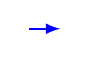
\begin{tikzpicture}
							\draw [color=blue,->,>=latex, thick](0,0)--(0.4,0);
						\end{tikzpicture}	 &$x'_1(t) = -\frac{1}{2}e^{-\frac{1}{2}t} \cos\left(\frac{\sqrt{47}}{2}t\right) - \frac{\sqrt{47}}{2}e^{-\frac{1}{2}t} \sin\left(\frac{\sqrt{47}}{2}t\right) $ \\
						$
						x_2(t) = e^{-\frac{1}{2}t} \sin\left(\frac{\sqrt{47}}{2}t\right)
						$	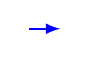
\begin{tikzpicture}
							\draw [color=blue,->,>=latex, thick](0,0)--(0.4,0);
						\end{tikzpicture}  &$
						x'_2(t) = -\frac{1}{2}e^{-\frac{1}{2}t} \sin\left(\frac{\sqrt{47}}{2}t\right) + \frac{\sqrt{47}}{2}e^{-\frac{1}{2}t} \cos\left(\frac{\sqrt{47}}{2}t\right)
						$
					\end{tabular}
					
					
					\begin{tabular}{ccc}
						$W(t) = \begin{vmatrix} x_1(t) & x_2(t) \\ x'_1(t) & x'_2(t) \end{vmatrix} ,
						$ & $W_1(t) = \begin{vmatrix} 0 & x_2(t) \\ f(t) & x'_2(t) \end{vmatrix} $ ,  & $W_2(t) = \begin{vmatrix} x_1(t) & 0 \\ f(t) & x'_1(t) \end{vmatrix}$ \\ 	
					\end{tabular}
				}
				
				\item {Al evaluar obtenemos los valores : 
					
					
					\[
					\begin{cases}
						W(t) = \sqrt{47} e^{-t} \\
						W_1(t) = -20e^{-\frac{1}{2}t} \sin(\frac{\sqrt{47}}{2}t) \cos(3t)\\
						W_2(t) = 20e^{-\frac{1}{2}t} \cos(\frac{\sqrt{47}}{2}t) \cos(3t)
					\end{cases}
					\]
					
					\[
					u_1' = \frac{ -x_2(t) f(t) }{ W(t) }, \quad u_2' = \frac{ x_1(t) f(t) }{ W(t) }
					\]
					
					Integrando para encontrar los valores de $u'_{1}$ y $u'_{2} $: 
					
					\[
					u_1(t) = \int \frac{-x_2(t) f(t)}{W(t)} \, dt , \quad u_2(t) = \int \frac{x_1(t) f(t)}{W(t)} \, dt
					\]
					
					Sumando los valores de $u'_{1}+ u'_{2} $:
					
					\[
					u_1 + u_2 = \int \frac{20 e^{-\frac{1}{2}t} \sin(\frac{\sqrt{47}}{2}t) \cos(3t)}{\frac{\sqrt{47}}{2} e^{-t}} \, dt + \int \frac{20 e^{-\frac{1}{2}t} \cos(\frac{\sqrt{47}}{2}t) \cos(3t)}{\frac{\sqrt{47}}{2} e^{-t}} \, dt
					\]
					
					\begin{marginfigure}
						\centering
						
						{\includegraphics[width=\marginparwidth]{Imagen/Resorte_3.pdf}}\\
						\caption{Solución de la $	u_1 + u_2 $}
						
						
					\end{marginfigure}
					
					Simplificando:
					
					\[
					u_1 + u_2 = \int \frac{40 e^{\frac{1}{2}t}\left[\sin(\frac{\sqrt{47}}{2}t)+\cos(\frac{\sqrt{47}}{2}t)\right]  \cos(3t)}{\sqrt{47}} \, dt 
					\]
					
				}
			\end{enumerate}
		}
	\end{enumerate}	
	
	
	
\end{sol}



\Example{Sistema Resorte/Masa Movimiento Forzado por función de Green }{
	Una masa que pesa 16 libras alarga \( \frac{8}{3} \) pie un resorte. La masa se libera inicialmente desde el reposo desde un punto 2 pies abajo de la posición de equilibrio y el movimiento posterior ocurre en un medio que ofrece una fuerza de amortiguamiento igual a \( \frac{1}{2} \) de la velocidad instantánea. Encuentre la ecuación de movimiento si se aplica a la masa una fuerza externa igual a \( f(t) = 10 \cos(3t) \).
}

\begin{marginfigure}
	\centering
	\subcaptionbox{Laplace}
	{\includegraphics[width=\marginparwidth]{Imagen/Resorte.pdf}}\\
	\subcaptionbox{Coeficiente indeterminado}
	{\includegraphics[width=\marginparwidth]{Imagen/Resorte_1.pdf}}\\
	\subcaptionbox{Por variación de parametro}
	{\includegraphics[width=\marginparwidth]{Imagen/Resorte_2.pdf}}
	\subcaptionbox{Cada gráfica segun el método utilizado para su solución}
	{\includegraphics[width=\marginparwidth]{Imagen/Resorte_4.pdf}}
	
	\caption{Comparación de solucines segun el método aplicado}
	
\end{marginfigure}

\begin{sol}
	\begin{enumerate}
		\item {Punto de partidad:	
			\[
			x'' + x' + 12x = 20 \cos(3t) ;  \quad	x(0) = 2, \quad x'(0) = 0
			\] 
			
		}
		
		\item{
			La solución $x_{c} $ :
			
			\[
			x_c = e^{\alpha t} \left( c_1 \cos(\beta t) + c_2 \sin(\beta t) \right)
			\] 
			
			\[
			x_c(t) = e^{-\frac{1}{2}t} \left( c_1 \cos\left(\frac{\sqrt{47}}{2} t\right) + c_2 \sin\left(\frac{\sqrt{47}}{2} t\right) \right)
			\] 
			
			\begin{enumerate}
				\item {Haciendo el cambio a la variable $s$:
					
					
					\begin{tabular}{cc}
						$
						x_1(t) = e^{-\frac{1}{2}t} \cos\left(\frac{\sqrt{47}}{2}t\right)
						$ 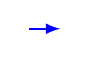
\begin{tikzpicture}
							\draw [color=blue,->,>=latex, thick](0,0)--(0.4,0);
						\end{tikzpicture}	 & $
						x_1(t) = e^{-\frac{1}{2}s} \cos\left(\frac{\sqrt{47}}{2}s\right)
						$ \\
						$
						x_2(t) = e^{-\frac{1}{2}t} \sin\left(\frac{\sqrt{47}}{2}t\right)
						$	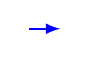
\begin{tikzpicture}
							\draw [color=blue,->,>=latex, thick](0,0)--(0.4,0);
						\end{tikzpicture}  &$
						x_2(t) = e^{-\frac{1}{2}s} \sin\left(\frac{\sqrt{47}}{2}s\right)
						$
					\end{tabular}
					
				}
				\item {Función de Green : 
					
					\[ G(t,s)= \frac{x_{1}(s) x_{2}(t)-x_{1}(t) x_{2}(s)}{W(s)}\] 
					
					\[G(t, s)= \frac{2e^{\frac{s-t}{2}} \sen(\frac{\sqrt{47}t-\sqrt{47}s}{2})}{\sqrt{47}} \]}
			\end{enumerate}
		}
		
		\item {Para encontrar $y_{p}$
			
			\[x_{p}(t)=\int_{t_0}^{t} G(t,s) F(s) ds  \]
			
			\[x_{p}(t)=\int_{t_0}^{t} \frac{40e^{\frac{s-t}{2}} \sen(\frac{\sqrt{47}t-\sqrt{47}s}{2}) cos(3s)}{\sqrt{47}} ds  \]
		}
	\end{enumerate}
	
\end{sol}

%%%%%%%%%%%%%%%%%%%%%%%%%%%%%%%%%%%%%%%%%%%
%\begin{tikzpicture}[
%	overlay, remember picture
%	]
	
%	\fill[gray!10]
%	([xshift = -8cm]current page.north east) --
%	([yshift = -5cm]current page.north east) |-
%	cycle;
	
%	\node[shift = {(-4cm,-2cm)}, opacity=0.3] at
%	(current page.north east)
%	{\includegraphics[scale = 4]{phys.pdf}};
	
%\end{tikzpicture}

%%%%%%%%%%%%%%%%%%%%%%%%%%%%%%%%%%%%%%%%%%%%%%%%






Aqui vamos hacer una prueba para romper el margen y ver que pasa .

\begin{comment}
\begin{fullwidth}[%
	width=16cm,
	outermargin=\dimexpr-\marginparsep-\marginparwidth,
	]
	\Teorema{Ecuación de Jacoby}{Esta es una prueba de numeracion}
	\Comentario{
		This is an example. \lipsum[1-2]
	}{
		What is truth? Can anything be proven?
	}
	
	
	
\end{fullwidth}
\end{comment}
%%%% Recordar que es para Imagenes con margen %%%%

\begin{comment}
	
	
\begin{figurefullwidth}
	\includegraphics[width=\dimexpr\textwidth+\marginparsep+\marginparwidth\relax]{4}
	\caption{This is a test caption}
	\label{fig:test1}
\end{figurefullwidth}

\end{comment}




%%%%%%%%%%%%%%%%%%%%%%%%%%%%%%%%%%%%%%


%\addcontentsline{toc}{subsection}{\protect\numberline{}Review}


%\addtocontents{toc}{\protect\vspace{1.0cm}}
